\chapter{Automatic annotation and scene parsing of UAV imagery and aerial imagery}
\label{ch:seg}
Last decade has witnessed a revolutionary success of deep neural networks. With the support of ever-increasing computing power, various deep neural networks have emerged for a wide range of applications and demonstrated significant improvements compared to traditional machine learning methods. Nevertheless, training the networks requires a large amount of ground truth data. While open image databases like ImageNet\cite{Russakovsky2015} and LabelMeFacade\cite{Russell2008} are only applicable for specific scenes, manual image annotating is usually inevitable and costs plenty of time and labor. Therefore increasing importance has been attached to the issue of automatic generation of image annotations. 

The prosperity of remote sensing brings about immense data of different scales and resolutions. The remotely sensed data, collected by a multitude of sensors (e.g., optical, hyperspectral, radar, LiDAR) from different platforms (e.g., satellite, airplane, UAV) and with different temporal intervals, conveys rich information of the scene from varying perspectives. Meanwhile, the coverage of free geographical information such as OSM is expanding rapidly. The way in which the redundant remote sensing data can be fully exploited is raising increasing attentions. In this context, we propose to exploit existing annotated data and incorporate auxiliary information from available remote sensing images to ease the task of image annotating. 

As a bridge between aerial and terrestrial photogrammetry, UAV images contribute to comprehensive representation of the scene. Pixelwise segmentation of UAV imagery is demanded by many applications such as building modeling, however, hand labelling of such a dataset is tedious and time consuming. In view of the fact that aerial images have much larger coverage than UAV images, we seek to propagate the labels from one aerial image to multiple co-registered UAV image. Theoretically, we simply need to annotate one aerial image manually and then transfer the labels to numerous UAV images of the same area, which would dramatically relieve the burden of manual annotation. 

There have been a couple of researches on label propagation, where labels are transferred  from sparse annotated data to a number of target images based on their temporal coherence and appearance similarity, e.g., across video frames or from point cloud to images. In these cases, the source data and target imagery have similar appearance and viewing direction, thus the propagation itself can result in fine image segmentations. In practice, however, such same-source data may not be available. When it comes to multi-source imagery, e.g., from aerial imagery to UAV imagery, the label propagation often suffers from large differences in  scale and view between source and target images and results in sparse, noisy and even wrong annotations. To solve this problem, we leverage geometric and radiometric information as additional features, and our problem can be formulated as how to reasonably infer the image labels given prediction uncertainties of multi-source information. Towards this goal, we introduce in this paper a Bayesian-CRF graphical model for accurate semantic segmentation incorporating features from both 2D images and 3D data. More specifically, the approach consists of three steps: 1. generate sparse weak annotations by propagating labels from existing labeled data; 2. model labeling uncertainties by introducing additional geometric and radiometric evidence via the Bayesian inference; 3. construct a densely connected CRF model on the image domain for label inference. The merits of the proposed method lie in the following aspects: 1. the probabilistic essence of our model allows for flexible incorporation of different types of auxiliary information; 2. our method is able to cope with missing labels and the ``dragging effect" in optical flow and achieves annotations with high semantic accuracy; 3. our method outperforms manual annotating in the aspect of preserving accurate class boundaries.  %joint reasoning of 2D and 3D information given weak annotations.

To verify the generalization and robustness of our method, we leverage it for two different applications: 1. UAV image annotating via label propagation from aerial to UAV imagery; 2. aerial image annotating via label propagation from OSM building footprints. In order to explore the effectiveness of deploying the automatically generated image annotations as pseudo ground truth, we train a deep convolutional neural network using these generated annotations for image segmentation, and compare with segmentation using manual annotations. 

To summarize, the main contributions of this work are:
\begin{itemize}
\item We present a novel concept of annotating UAV imagery by transferring the labels from existing annotated aerial imagery.
\item We propose a Bayesian-CRF graphical model which can flexibly incorporate 2D and 3D features as auxiliary information, yielding refined image annotations. 
\item We demonstrate the effectiveness of these annotations as pseudo ground truth data for training deep neural works for image segmentation.
\end{itemize}

The remainder of this paper is organized as follows: Section \ref{sec:related} compares related research work and highlights the innovations of our method. Section \ref{sec:method} describes the proposed framework in details. Section \ref{sec:experiment1} and Section \ref{sec:experiment2} present the applications of the proposed method in different scenarios and report the experimental results with evaluations. Section \ref{sec:disc} interprets the results and describes applicable conditions of the proposed method. Finally, Section \ref{sec:conc} concludes the paper.
% You must have at least 2 lines in the paragraph with the drop letter
% (should never be an issue)
\section{Related work}
\label{sec:related}
% In this section, we give an review of related works on label propagation, followed by a brief introduction of CRF model. We also highlight the innovations of our study compared with previous works.

In order to tackle the lack of annotated data, a couple of attempts have been made in automatic generation of image annotations. One option is to generate synthetic data. The emergence of synthetic datasets like Virtual KITTI \cite{gaidon2016virtual} and Synthia \cite{Ros2016synthetic} reveals its potential in generating image annotations on a large scale, but the quality of synthetic data largely relies on the quality of the generative model. Though such models can find regular patterns of the authentic data, they may not be able to generate distinctive and diverse images like realistic data, which is a severe limitation for most training tasks.
%However, for most training tasks, the synthetic data will severely limit its capabilities and negatively impact the output accuracy. 

An effective way of automatic image annotation is label propagation, i.e., transfer the pixel labels from source data to target images via certain correspondences. A common case is propagation throughout video frames. Naive methods use optical flow to model the frame to frame propagation \cite{chuang2002video} but often suffer from occlusion and reappearance of objects. To handle this problem, more sophisticated appearance models have been proposed, such as local shape models in \cite{Bai2009snapcut}, semantically consistent regions in \cite{arbelaez2009regions} and patch cross-correlation in \cite{badrinarayanan2013semi}. Unstructured classifiers, which predict pixel labels independently without neighborhood constraints, mostly use Random Decision Forests \cite{Breiman2001random} and CRFs to get the unaries. While structured classifiers involve neighborhood information to improve segmentation accuracy. For example, a coupled HMM was proposed in \cite{badrinarayanan2010label} for joint generative modeling of image sequences and their annotation. Some works \cite{Tsai2012motion},\cite{wang2009active} used joint optimization for temporal motion and semantic labels. A mixture of trees probabilistic graphical model was employed in \cite{badrinarayanan2013semi} for temporal association between super-pixels, which can reduce errors caused by short time-window processing in label propagation.

Due to lack of depth information, video-based label propagation approaches are vulnerable to occlusions. In contrast, some methods exploited 3D information as source data for label propagation. For example, the approach presented in \cite{chen2014beat} exploited 3D information including stereo, noisy point clouds, 3D car models as well as appearance models to generate accurate vehicle segmentation. Xiao et al \cite{multiple2009} proposed to generate street view image segmentation by projecting 3D annotations onto image superpixels and optimizing the results in a MRF model. However, as the point cloud was generated from Structure from Motion (SFM), this method still had difficulty in dealing with occlusions. In comparison, the hybrid methods presented in \cite{namin2015multimodal},\cite{Xie2016CVPR} jointly inferred 2D imagery and 3D point clouds in graphical models and demonstrated improvements in the semantic labeling of both modalities. 
% As we are interested in image annotations, labeling of point cloud is not the main concern, thus we use the 3D data solely as auxiliary evidence rather than an independent domain for the sake of relieving computational burden.
% As we start from only 2D image annotations and target at generating image annotations, the 3D labeling is not the main concern for us, therefore   


Aforementioned methods demonstrate that incorporation of multi-view information can help to improve segmentation accuracy and temporal consistency of annotations, thus, we are inspired to exploit additional radiometric and geometric information for the label propagation task. Nevertheless, existing methods mainly work with label propagation between same-source data, e.g., across video frames or from terrestrial point cloud to street-view images, where the source data and target imagery have high similarity in view and appearance. However, when it comes to multi-view imagery, the labels propagation suffers from view differences between source data and target images, resulting in sparse and erroneous annotations. For instance, building facades in UAV imagery are often invisible in aerial imagery and thus cannot be annotated, direct label propagation would result in missing labels on the facade area of UAV images. We tackle this problem in a different way: assuming that corresponding nodes in 2D and 3D domains have identical labels, we update the unary potential of each node with Bayesian inference given evidence (e.g., height, normal vector, NDVI) from auxiliary data, where the likelihood is empirically estimated based on image statistics. In that example, we can encourage the 3D node whose normal vector is horizontal to be "facade" by assigning them a higher likelihood.   

Learning and inference of CRF models for semantic segmentation have already been discussed by many previous research works. Basic CRF models only consider neighboring pixels or patches \cite{shotton2009textonboost},\cite{fulkerson2009Class}, which cannot handle long-range connections within the image and often lead to over-smoothing at class boundaries. To solve this problem, higher-order CRFs \cite{Kohli2008robust} and hierarchical CRFs \cite{Ladicky2009hierarchical} have been proposed to integrate region-based hierarchical connections and higher-order potentials, yet the accuracy of such methods largely depend on the accuracy of segmented image regions. By contrast, fully connected CRFs incorporate pairwise potentials for all individual pixels in the image, resulting in significantly higher segmentation accuracy. To reduce the computational complexity of inference, the mean-field inference algorithm for fully connected CRF models has been proposed in \cite{crf2012}, where, the pairwise edge potentials are defined as a weighted sum of Gaussian kernels and the message passing is performed using Gaussian filtering in a Euclidean feature space, enabling highly efficient maximum posterior marginal (MPM) inference. To the best of our knowledge, we are the first to employ such CRF models for label propagation between multi-source images.
% Specifically, loopy belief propagation was proposed in \cite{Ren2008}, tree reweighted belief propagation was described in \cite{choi2013fpga} 
 

Despite many works on label propagation, few of them have investigated into the possibility of using the propagated labels as pseudo ground truth for training at scale. A notable exception is the work in \cite{mustikovela2016can}, where a systematic analysis about the quality of PGT was presented and the impact of PGT on training a CNN was discussed. Similarly, the effect of large scale PGT on deep learning based segmentation is investigated in \cite{large2017}. In such cases, the propagated annotations were merely employed as augmented ground truth data and trained together with manually labeled ground truth. By contrast, we demonstrate that the automatic annotations generated by our method can be directly used as ground truth data and achieve comparable accuracy in CNN based segmentation as manual annotations.
% needed in second column of first page if using \IEEEpubid
%\IEEEpubidadjcol

\section{Methodology}
\label{sec:method}
% In this section, we first formulate our problem, and then give a detailed description of the proposed model.
Label propagation methods transfer labels from annotated source data to a set of target images. In practice, the source annotated data can be aerial imagery, satellite imagery, OSM data, etc. Here we take the case of label propagation from aerial imagery to UAV imagery as an example.

For existing label propagation methods, the source data and target imagery are temporally coherent and similar in view and appearance, e.g., across video frames or from point cloud to images, where the propagation itself can result in accurate image annotations. In our case, the source and target images differ considerably in the aspects of scale, viewing direction, illumination, etc, as UAV imagery is taken at lower altitude with a more oblique view than in aerial imagery. Consequently, the label propagation often results in sparse, noisy and erroneous annotations. In this context, our task can be formulated as a weakly supervised image segmentation problem. 

Figure \ref{fig:eichenau_transferred} shows an example of the annotations of UAV imagery transferred from aerial imagery, many labels are missing at occluded regions, especially at building facades. Such missing labels are difficult to identify using only color and texture information, but can be distinguished based on auxiliary geometric and 3D features. Intuitively, normal vectors of building facades are generally horizontal while those of the ground are vertical, roofs are expected to be higher than cars, and vegetations appear deeper red in the near-infrared band. The implicit mathematical essence behind is that each object has a distinctive distribution regarding a certain geometric or radiometric attribute. Such distributions, if properly incorporated as auxiliary features, can substantially contribute to a better segmentation accuracy. To this end, we incorporate these auxiliary features from available remote sensing data, and construct a densely connected Bayesian-CRF model to reason about the labels based on evidence. 
% In order to explain our methodology more concretely. So the procedure of label transfer will be omitted in this chapter and explained in Section \ref{sec:experiment1}, here we take the case of label propagation from aerial imagery to UAV imagery as an example. By contrast, we aim to generate UAV image annotations by transferring labels from aerial imagery to UAV imagery.


\subsection{Model}
A CRF can be seen as a Markov Random Field (MRF) globally conditioned on the data. In the context of image segmentation, a CRF models pixel labels as random variables which have a Markov property and are conditioned upon the image.

More formally, for an input image of size N, consider a set of random variables $\mathbf{X} = \{X_1,\dots, X_N\}$ ranging over the image, where $X_i$ denote the label assigned to pixel $i$ and the value is taken from a set of pre-defined semantic labels $\mathcal{L} = \{l_1, \dots, l_K\}$. For a global observation (image) $\mathbf{I}$, consider a graph $G = \left(V, E\right)$, where $V = \{X_1,\dots, X_N\}$, the pair (\textbf{I}, \textbf{X}) can be modeled as a conditional random field which is characterized by a Gibbs distribution $P\left(\textbf{X}=\textbf{x} \mid \textbf{I}\right) = \frac{1}{Z\left(\textbf{I}\right)} \exp \left( - E\left(\textbf{x} \mid \textbf{I}\right)\right)$, where $\mathbf{x} \in \mathcal{L}$ and $Z\left(\textbf{I}\right)$ is the partition function. Assume the conditional random field ($\mathbf{I},\mathbf{X}$) is fully connected, the energy of a label assignment $\textbf{x}$ is specified as:

% More formally, for input images of size N, consider a random field $\mathbf{I} = \{I_1,\dots, I_N\}$ ranging over image pixels, $I_j$ denote the color value of pixel $j$. Consider also a random field $\mathbf{X} = \{X_1,\dots, X_N\}$ ranging over pixel-wise labels, $X_j$ denote label of pixel $j$. Let $\mathbf{L} = \{l_1, \dots, l_k\}$ denote the domain the set of labels. Assume the conditional random field ($\mathbf{I},\mathbf{X}$) is fully connected, its corresponding Gibbs energy is specified as:
\begin{align} \label{eq:1}
E\left(\mathbf{x}\right) &= \sum_{i}^{} \psi_u\left(x_i\right) + \sum_{i<j}^{} \varphi_p\left(x_i,x_j\right)
\end{align}

% \begin{figure}[htb]
%     \centering
%        \begin{subfigure}[b]{1\linewidth}
% 	       \centering
% 			\newcommand{\myGlobalTransformation}[2]
{
    \pgftransformcm{1}{0}{0.3}{0.5}{\pgfpoint{#1cm}{#2cm}}
}

% draw a 4x4 helper grid in 3D
% Input: point of origins x and y coordinate and additional drawing-parameters
\newcommand{\gridThreeD}[3]
{
    \begin{scope}
        \myGlobalTransformation{#1}{#1};
        \draw [#3,step=2cm] grid (6,6);
    \end{scope}
}

\tikzstyle myBG=[line width=3pt,opacity=0.0]

% draws lines with white background to show which lines are closer to the
% viewer (Hint: draw from bottom up and from back to front)
%Input: start and end point
\newcommand{\drawLinewithBG}[2]
{
    \draw[white,myBG]  (#1) -- (#2);
    \draw[black,thick] (#1) -- (#2);
}

% draws all horizontal graph lines within grid
\newcommand{\graphLinesHorizontal}
{
    \drawLinewithBG{1,1}{5,1};
    \drawLinewithBG{1,1}{5,3};
    \drawLinewithBG{1,1}{1,5};
    \drawLinewithBG{1,1}{3,5};
    \drawLinewithBG{1,1}{5,5};
    \drawLinewithBG{1,3}{5,3};
    \drawLinewithBG{1,3}{3,3};
    \drawLinewithBG{1,3}{3,1};
    \drawLinewithBG{1,3}{5,1};
    \drawLinewithBG{1,3}{3,5};
    \drawLinewithBG{1,3}{5,5};
    \drawLinewithBG{1,5}{5,5};
    \drawLinewithBG{1,5}{5,3};
    \drawLinewithBG{3,1}{3,5};
    \drawLinewithBG{3,1}{1,5};
    \drawLinewithBG{3,1}{5,3};
    \drawLinewithBG{3,1}{5,5};
    \drawLinewithBG{5,1}{5,5};
    \drawLinewithBG{5,1}{1,5};
    \drawLinewithBG{5,1}{3,5};
    \drawLinewithBG{5,3}{3,5};
}

% draws all vertical graph lines within grid
\newcommand{\graphLinesVertical}
{
    %swaps x and y coordinate (hence vertical lines):
    \pgftransformcm{0}{1}{1}{0}{\pgfpoint{0cm}{0cm}}
    \graphLinesHorizontal;
}

%draws nodes of the grid
%Input: point of origins x and y coordinate
\newcommand{\graphThreeDnodes}[2]
{
    \begin{scope}
        \myGlobalTransformation{#1}{#2};
        \foreach \x in {1,3,5} {
            \foreach \y in {1,3,5} {
            \draw[fill=white,color=yellowgreen] (\x,\y) circle [radius=0.2cm];
            \node{};            
                %\node at (\x,\y) [circle,radius=1cm,fill=green] {};
                %this way circle of nodes will not be transformed
            }
            \node at (0.5,1) {$O_i$}; 
        }
    \end{scope} 
    \begin{scope}
        \myGlobalTransformation{#1}{#1};
        \foreach \x in {1,3,5} {
            \foreach \y in {1,3,5} {
            \draw[fill=white,color=royalblue] (\x,\y) circle [radius=0.2cm];
            
            \node{};
                %\node at (\x,\y) [circle,fill=blue] {};
                %this way circle of nodes will not be transformed
            }
            \draw[fill=white,color=white] (0.5,1) circle [radius=0.2cm];;
            \node at (0.5,1) {$\textbf{X}$};         
        }
    \end{scope}       
}


\pagestyle{empty}

\begin{tikzpicture}

    %draws helper-grid:
    \gridThreeD{0}{0}{black!50};
    \gridThreeD{0}{3.25}{black!50};

    %draws lower graph lines and those in z-direction:
    \begin{scope}
        \myGlobalTransformation{0}{0};
        \graphLinesHorizontal;

        %draws all graph lines in z-direction (reset transformation first!):
        \foreach \x in {1,3,5} {
            \foreach \y in {1,3,5} {
                \node (thisNode) at (\x,\y) {};
                {
                    \pgftransformreset
                    \draw[white,myBG]  (thisNode) -- ++(0,3.25);
                    \draw[black,very thick] (thisNode) -- ++(0,3.25);
                }
            }
        }
    \end{scope}

    %draws upper graph-lines:
    \begin{scope}
        \myGlobalTransformation{0}{3.25};
        %\graphLinesVertical;
    \end{scope}

    % draws all graph nodes:
    \graphThreeDnodes{0}{0};
    \graphThreeDnodes{0}{3.25};

\end{tikzpicture}%
			
%        \end{subfigure}
%        \caption{Proposed graph model.}
%        \label{fig:graph}
% \end{figure}
The unary potentials $\psi_u\left(x_i\right)$ encode the probability of a pixel $i$ taking label $x_i$. In our case, pixel-wise label assignment probabilities are initially defined according to the accuracy  $p$ of the transferred weak annotations. For instance, for an image segmentation task in five categories $\{Building, Ground, Vegetation, Car, Clutter\}$, we believe the transferred annotations have 80\% accuracy, i.e., the value of $p$ is set to 0.8. If a pixel is labeled as $Ground$ in the transferred annotation, then the prior label assignment probability for this pixel is represented as a vector of probabilities for each class: $\{0.05, 0.8, 0.05, 0.05, 0.05\}$. In case the pixel is not assigned any label, the a priori of label assignment is set to the average value: $\{0.2, 0.2, 0.2, 0.2, 0.2\}$. % Due to occlusions, however, some pixels may have wrong labels, no labels or multiple labels, especially for classes \textit{Building} and \textit{Car}. To solve this problem, we exploit geometric information embedded in 3D points such as height and normal vectors. At ambiguous regions, these complimentary features can help to distinguish different classes. In parallel, the energy of each node is simultaneously affected by the evidence of additional features. 
Further, the pixel-wise label assignment probabilities are then updated via Bayesian inference given additional evidence. More specifically, given a sequence of independent and identically distributed evidence features (e.g., height, normal vector, spectral information): $\mathbf{O} = \{O_1, \dots, O_m\}$, where $m$ stands for the number of features. 
% As illustrated in Figure \ref{fig:graph}, blue nodes represent pixel labels fully connected with each other, green nodes stand for additional geometric features $\{O^1_i,\dots,O^m_i\}$. 
Let $P\left(\mathbf{x}\right)$ denote the prior belief of the transferred annotation and $P\left(\textbf{O}\mid \mathbf{x}\right)$ denote the likelihood of observing $\textbf{O}$ given category $\mathbf{x}$. In our experiment, the value of $P\left(\textbf{O}\mid \mathbf{x}\right)$ is empirically defined based on image statistics. The posterior probability of label assignment $\mathbf{x}$ for given evidence set $\mathbf{O}$ can be inferred based on Bayes' theorem \cite{gelman2013bayesian}:
\begin{equation}
\label{eq:2}
%\varphi_p\left(x_i\mid O \right) = \frac{P(O \mid x_i)P\left(xi\right)}{P(O)}
% P\left(x_i\mid O^1_i,\dots,O^m_i \right) = \frac{1}{Z}P\left(x_i\right)\prod_{j=1}^{m}P\left(O^j_i \mid x_i\right)
P\left(\mathbf{X}=\mathbf{x}\mid \mathbf {\mathbf{O}} \right)=\frac {P\left(\mathbf {O} \mid \mathbf{x}\right)}{\sum_{\mathbf{x}\in \mathcal{L}}{P\left(\mathbf {O} \mid \mathbf{\mathbf{x}}\right)P\left(\mathbf{x}\right)}}\cdot P\left(\mathbf{x}\right)
\end{equation}
where, 
\begin{equation}
\label{eq:3}
P\left(\mathbf {O} \mid \mathbf{x}\right)=\prod _{m}{P\left(O_m\mid \mathbf{x}\right)} 
%\varphi_p\left(x_i\mid O \right) = \frac{P(O \mid x_i)P\left(xi\right)}{P(O)}
% Z = P\left(O\right) = \sum_{i=1}^{N}P\left(x_i\right)P\left(O \mid x_i\right)
\end{equation}


% For the sake of notation consistency, we will use $\psi_u\left(x_i\right)$ instead of $P\left(X\mid O \right)$ in the following part of text.

Pairwise potentials $\varphi_p\left(x_i, x_j\right)$ encode the cost to assign labels $x_i, x_j$ to pixels $i, j$ respectively, the data-dependent term encourages semantic label coherence of similar pixels. Following the settings in \cite{crf2012}, we model the pairwise term as weighted contrast-sensitive Gaussian edge kernels: 
% \begin{equation}
\begin{multline} \label{eq:4}
%\varphi_p(x_i,x_j) &= \mu(x_i,x_j) \sum_{m=1}^{K} \omega ^{(m)}\kappa ^{(m)}(f_i,f_j),
\varphi_p\left(x_i,x_j\right) = \omega_1\left(x_i,x_j\right) exp\left(-\frac{\mid p_i-p_j\mid ^2}{2{\theta_\gamma}^2}\right) \\
 +\omega_2\left(x_i,x_j\right) exp\left(-\frac{\mid p_i-p_j\mid ^2}{2{\theta_\alpha}^2} -\frac{\mid c_i-c_j\mid ^2}{2{\theta_\beta}^2} \right)
\end{multline}
% \end{equation}
where $c_i$ and $p_i$ represent the color vector and position of pixel $i$ respectively, $\omega_1$ and $\omega_2$ parametrizes the weights of pairwise features and are both set to 1 in our model. Further, $\theta_\alpha$, $\theta_\beta$ and $\theta_\gamma$ control the degree of nearness, similarity and smoothness and are set to 25, 10, 3 respectively in our model.
%The parameter values in our experiment are 20, 8, 3 respectively.
% The parameter values in our experiment are $\theta_\alpha = 20$, $\theta_\beta=8$, $\theta_\gamma=3$ respectively.

The pseudo code of the proposed method is listed in Table \ref{tab:pseudo}, which demonstrates the general pipeline and explains the Bayesian-based inference in details. 
\begin{algorithm}
\caption{Bayesian-CRF Based Image Annotation}\label{tab:pseudo}
     \textbf{Input:} Image $\mathbf{I}$, degree of belief for the transferred annotations $p$, number of categories $K$, auxiliary evidence set $\mathbf{O}$, likelihood function $P\left(\mathbf{O}\mid \mathbf{x}\right)$\\
     \textbf{Output:} Pixel-wise annotation of image $\mathbf{I}$
    \begin{algorithmic}[1]
    \Procedure{Update pixel unary potentials based on additional measurement}{}
      \For{each pixel $i$ in $\mathbf{I}$}      
        \State $O \gets$ observation measurement for this pixel.
        \State $P\left(x_i\right) = [P_1,\dots,P_K]^{T} \gets $ prior label assignment probability of this pixel.
     	\If {pixel $i$ is not assigned any label via transferring}
         \State $P\left(x_i\right) = [\frac{1}{K},\dots,\frac{1}{K}]^{T}$.
      	\Else        
     	\State $k \gets$ index number of transferred label.
     	\For {each $P_j (j=1,\dots,K)$ in vector $P\left(x_i\right)$}
        \If {$j \neq k$}
        $P_j = \frac{1-p}{n-1}$
        \Else 
        \State $P_j = p$
        \EndIf
        \EndFor
        
     	\EndIf
%         \For{each per-class a priori $P_j$ in $P$}
%         \State $P\left(O \mid x\right) \gets $ likelihood of the measurement $O$ for given class $x$.  
    	\State $P\left(x_i\mid O\right) = \frac{P\left(x_i\right)\cdot P\left(O \mid x_i\right)}{P\left(O\right)} \gets $ posterior label assignment probability updated by Bayes' theorem.
%         \EndFor
      \EndFor
      \State
%     \State $\textit{stringlen} \gets \textit{length of } \textit{string}$
%     \State $i \gets \textit{patlen}$
%     \BState \emph{top}:
%     \If {$i > \textit{stringlen}$} \Return false
%     \EndIf
%     \State $j \gets \textit{patlen}$
%     \BState \emph{loop}:
%     \If {$\textit{string}(i) = \textit{path}(j)$}
%     \State $j \gets j-1$.
%     \State $i \gets i-1$.
%     \State \textbf{goto} \emph{loop}.
%     \State \textbf{close};
%     \EndIf
%     \State $i \gets i+\max(\textit{delta}_1(\textit{string}(i)),\textit{delta}_2(j))$.
%     \State \textbf{goto} \emph{top}.
    \EndProcedure
    
    \Procedure{Semantic inference in CRF model}{}
%     \State $\mathbf{I} = \{I_1,\dots, I_N\} \gets$ a random field  defined over $\mathbf{M}$
    \State $ E =$ pixel unary potentials + pixel pairwise potentials$\gets$  Gibbs energy function 
    \State Inference by minimizing $E$ 
    \EndProcedure 
    \end{algorithmic}
    \end{algorithm}


\subsection{Inference}
\label{method:infer}
The inference problem is basically to find the label assignment $\mathbf{x}$ with the maximum a posteriori (MAP) of a random field for the given image $\mathbf{I}$, i.e., $X\ast = argmax_{\mathbf{x}\in\mathcal{L}}P(\mathbf{x}\mid \mathbf{I})$, and can be achieved by minimizing the Gibbs energy function $E\left(\mathbf{x}\right)$. The time for solving the maximization of these marginals is exponential in the size of $\mathbf{I}$ and thus computationally intractable. Therefore we employ the mean field approximation for the maximum posterior marginal inference, i.e., approximating the exact CRF distribution $P(\mathbf{X})$ with a factorized distribution $Q(\mathbf{X}) = \prod_{i}Q_i(X_i)$ that minimizes the KL-divergence $D(P\|Q)$. The mean field approximation can be performed using Gaussian filtering in feature space efficiently \cite{crf2012}.

% \subsection{Learning}
% We learn the parameters by maximum likelihood, i.e., the parameters setting should have highest probability given the training data. However, maximum likelihood training of a CRF model is intractable in general cases. So we resort to approximate inference methods, as discussed in Section \ref{method:infer}. 

% In order to estimate the parameters, we compute the marginal distribution for each edge. 
% In the end, the parameters in our CRF model are learned via minimization of the Gibbs energy defined in Eq. 

\section{image annotation via label propagation from aerial imagery to UAV imagery}
\label{sec:experiment1}
In this section, we leverage the proposed method to generate pseudo ground-truth data for training. The experiments are comprised two aspects: 1. image annotating via label propagation from aerial imagery to UAV imagery, 2. training a CNN using the generated annotations. We describe data acquisition, introduce experiment settings, present and evaluate the results. 
%2.automatic building annotation of aerial images using OSM footprint. 

%\subsection{Experiment 1: automatic image annotation via label propagation}
\subsection{Data Description}
As shown in Figure \ref{fig:site}, this dataset consists of two subsets: \textbf{Area 1} was acquired over \texttt{Eichenau}, a small village in Germany. It is characterized by dense anthropogenic structures such as traditional-style houses, dense vegetations, roads and moving cars; \textbf{Area 2} was acquired over a nearby village \texttt{Unterroggenstein}, including a few detached buildings along the roadside. 

Image data were taken on November $2^{nd}$, 2015. In particular, UAV imagery was captured by a Sony Nex-7 camera at an altitude of $100m$ above ground with a slightly oblique view. The average Ground Sampling Distance (GSD) of UAV images is 1.8cm and the image size is $6000 \times 4000$ pixels; aerial imagery was acquired by the DLR 4k sensor system \cite{kurz2014performance} at an altitude of $600m$ above ground, including two Canon EOS-1DX cameras with 15$^\circ$ sidewards looking angle and a FOV of 75$^\circ$ across. The aerial imagery has an average GSD of 20cm and size of $5184 \times 3456$ pixel. \textbf{Area 1} is covered by both aerial imagery and UAV imagery while \textbf{Area 2} is only covered by UAV imagery. 
Detailed characteristics of the datasets are listed in Table \ref{tab:dataset}.
\begin{table}[htb]
\centering
\begin{tabular}{cccccc}
\toprule
Imagery  & Date & Size (pixels) & Height (m) & GSD (cm) & Pitch ($^{\circ}$) \\
\midrule
Aerial  & 11/2015 & $5184 \times 3456$ & 600 & 8.4 & 15 \\
UAV     & 11/2015 & $6000 \times 4000$ & 100 & 1.8 & 10\\
\bottomrule
\end{tabular}
\caption{Characteristics of the datasets used in the experiment.}
\label{tab:dataset}
\end{table}

We defined six classes for this dataset, i.e., \textit{Building}, \textit{Roof}, \textit{Ground}, \textit{Vegetation}, \textit{Car} and \textit{Clutter}. Where, class \textit{Building} refers to building facades; class \textit{Roof} refers to roofs (including overhangs); class \textit{Ground} refers to bare grounds and roads; class \textit{Vegetation} includes trees, bushes and grassland; class \textit{Car} includes all types of vehicles; the rest categories and indistinguishable objects belong to class \textit{Clutter}. The color coding for labels is illustrated in Figure \ref{fig:colorbar_ei}.
\begin{figure}[htb]
    \centering
\begin{subfigure}{0.9\columnwidth}
  \centering
  
\includegraphics[width=1\linewidth]{fig/eichenau/colorbar.JPG}
\end{subfigure} 
\caption{Color coding used for label propagation from aerial to UAV imagery}
       \label{fig:colorbar_ei}
\end{figure} 

From \textbf{Area 1}, two aerial images were manually annotated as source-data for label propagation, costing about 60-90 minutes per frame; in order to compare with the automatically inferred annotations, we manually labeled 28 UAV images as ground-truth data, costing about 20-30 minutes per frame, and then split them into 23 training samples and 5 testing samples. \textbf{Area 2} is only used for testing.

\begin{figure}[htb]
    \centering
       \begin{subfigure}[b]{1\linewidth}
	       \centering
			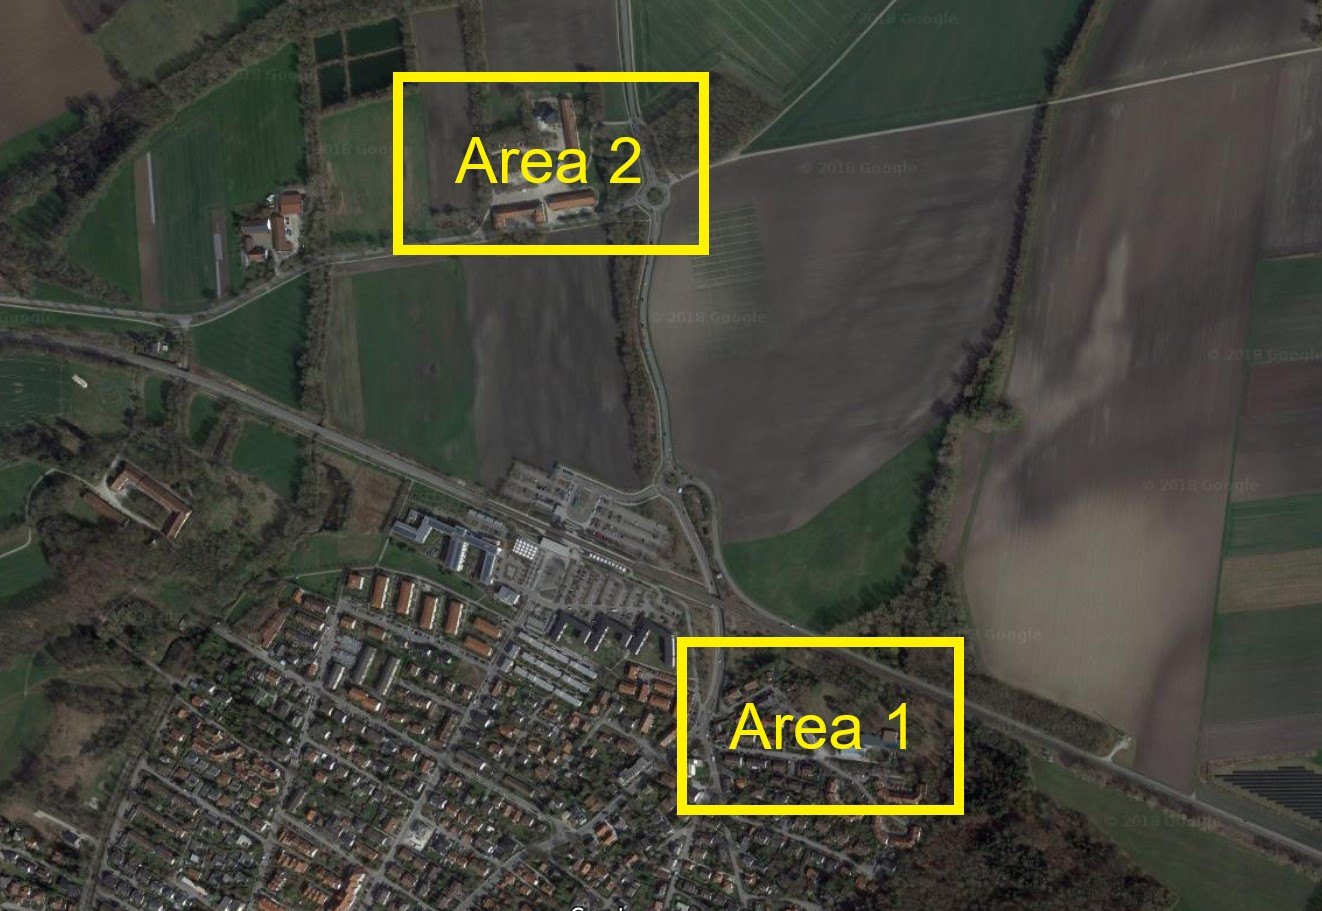
\includegraphics[width=0.8\textwidth]{fig/eichenau/site.JPG}
       \end{subfigure}
       \caption{Location of two survey sites \textbf{Area 1} (Eichenau) and \textbf{Area 2} (Unterroggenstein), Germany.}
       \label{fig:site}
\end{figure} 

\subsection{Data Pre-processing}
A high co-registration accuracy is vital to the label propagation between multi-source image data. As the UAV images in our dataset exhibit a much lower geolocalization accuracy than aerial images, we adopted the approach proposed in \cite{zhuo2017automatic} for co-registration between UAV and aerial images. In short, the method assumes that the aerial images are geo-referenced and have common overlap with UAV images. First, the camera poses of sequential UAV images are solved via Structure From Motion (SFM), and then the nadir UAV images are matched with the aerial images using the proposed matching scheme and generate thousands of reliable image correspondences. Given accurate camera poses of the aerial images, the 3D coordinates of those common image correspondences can be calculated via image-to-ground projection. These 3D points are then adopted to estimate the camera poses of the corresponding nadir-view UAV images. In the end, those UAV images with known camera poses are involved in a global optimization for camera poses of all UAV images. In this way, all UAV images are co-registered to the aerial images with pixel-level registration accuracy. Afterward, we reconstruct UAV point cloud and Digital Surface Model (DSM) using software \textit{Pix4Dmapper Pro} (version 4.0.25), and then generate a heightmap for each UAV image by deriving heights from the DSM.

Annotated pixels in aerial imagery can be transferred to UAV imagery based on their orientation parameters. However, individual aerial imagery does not present the same scene as UAV imagery due to their temporal difference and differences in viewing direction, scale, resolution and illumination, etc. For instance, building facades in UAV images maybe not or only partially visible in aerial images. Thus we labeled two aerial images, one left-view and one right-view, to achieve more complete representation of the scene. Figure \ref{fig:3k_uav} depicts an oblique UAV imagery and the corresponding region in left-view and right-view aerial images. It can be seen that the combination of the two views can compensate for the view difference to some extent. 
% yet there are still substantial differences between the UAV and aerial imagery such as scale, resolution and illumination, which are quite challenging for the label propagation task. 

\begin{figure}[htb]
\begin{minipage}[b]{0.32\linewidth}
  \centering
  \centerline{\epsfig{figure=fig/eichenau/DSC00838.JPG,width=2.8cm}}
  \centerline{(a)}
\end{minipage}
\begin{minipage}[b]{0.32\linewidth}
  \centering
  \centerline{\epsfig{figure=fig/eichenau/R0414_crop.png,width=2.8cm}}
  \centerline{(b)}
\end{minipage}
\hfill
\begin{minipage}[b]{0.32\linewidth}
  \centering
  \centerline{\epsfig{figure=fig/eichenau/R0845_crop.png,width=2.8cm}}
  \centerline{(c)}
\end{minipage}
\hfill
\caption{Comparison of aerial imagery and UAV imagery. (a) UAV image, (b) corresponding region in left-view aerial image, (c) corresponding region in right-view aerial image}
\label{fig:3k_uav}
\end{figure}

% The two selected aerial images were manually labeled to five main categories: \textit{Building}, \textit{Roof}, \textit{Ground}, \textit{Low vegetation} and \textit{Car}. A few indistinguishable objects were labeled as \textit{Clutter} and will be ignored in training. 


\subsection{Label Transfer}
As explained in Section \ref{sec:method}, we use the UAV point cloud as a mediator for label propagation. To be more specific, we project all the 3D points into a labeled aerial image, thus all the non-occluded points get labeled, and then we project these 3D points into UAV images, transferring their labels to corresponding image pixels. Figure \ref{fig:color_pc} illustrates the labeled UAV point cloud, where, (a) shows labels transferred from the left-view aerial image and (b) shows labels transferred from the right-view aerial image. It can be seen that the combination of two aerial images contributing to more enriched and complete representation of the scene.     

\begin{figure}[H]
\begin{subfigure}{0.49\columnwidth}
  \centering
  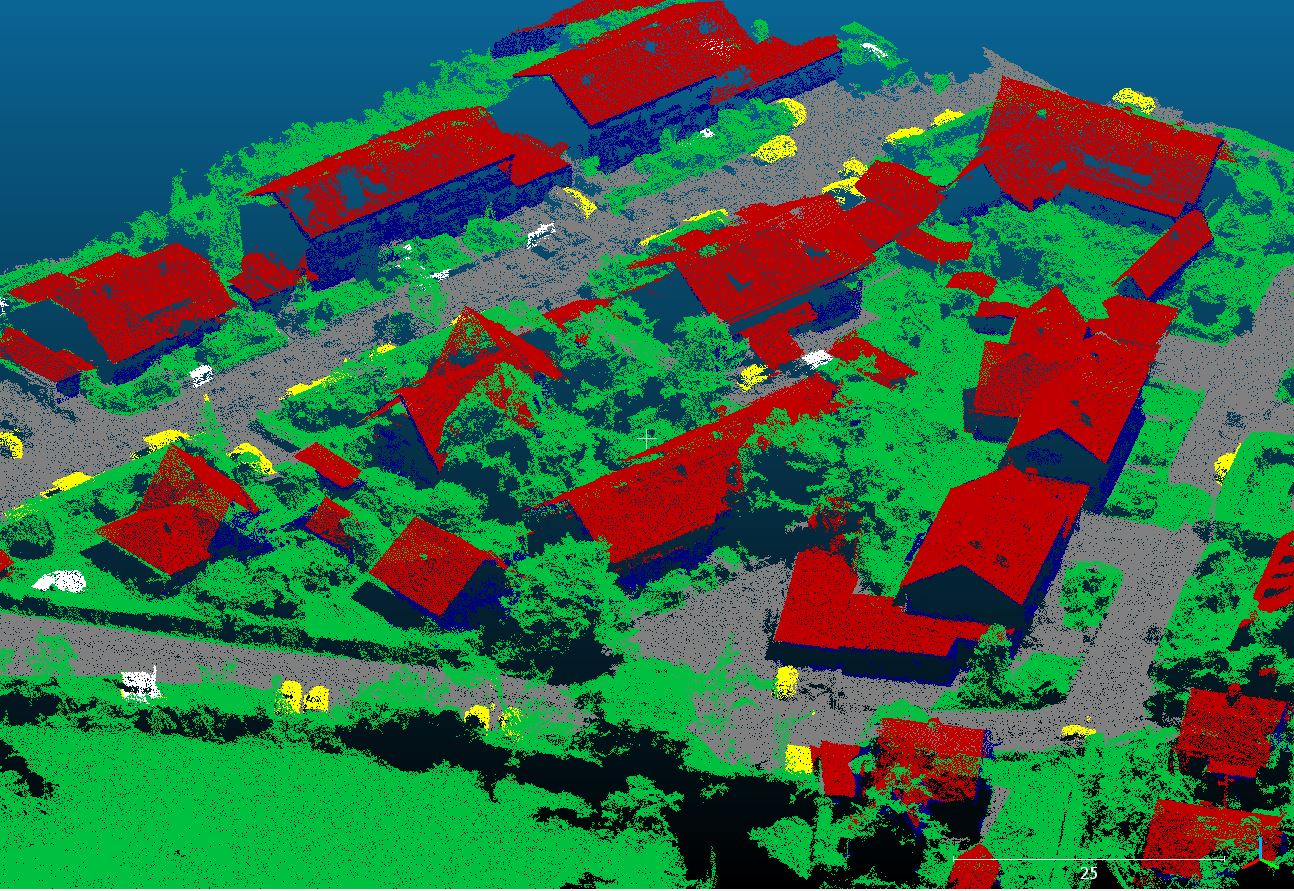
\includegraphics[width=1\linewidth]{fig/eichenau/pc_colored_l.JPG}
  \caption{}

\end{subfigure}
\begin{subfigure}{0.49\columnwidth}
  \centering
  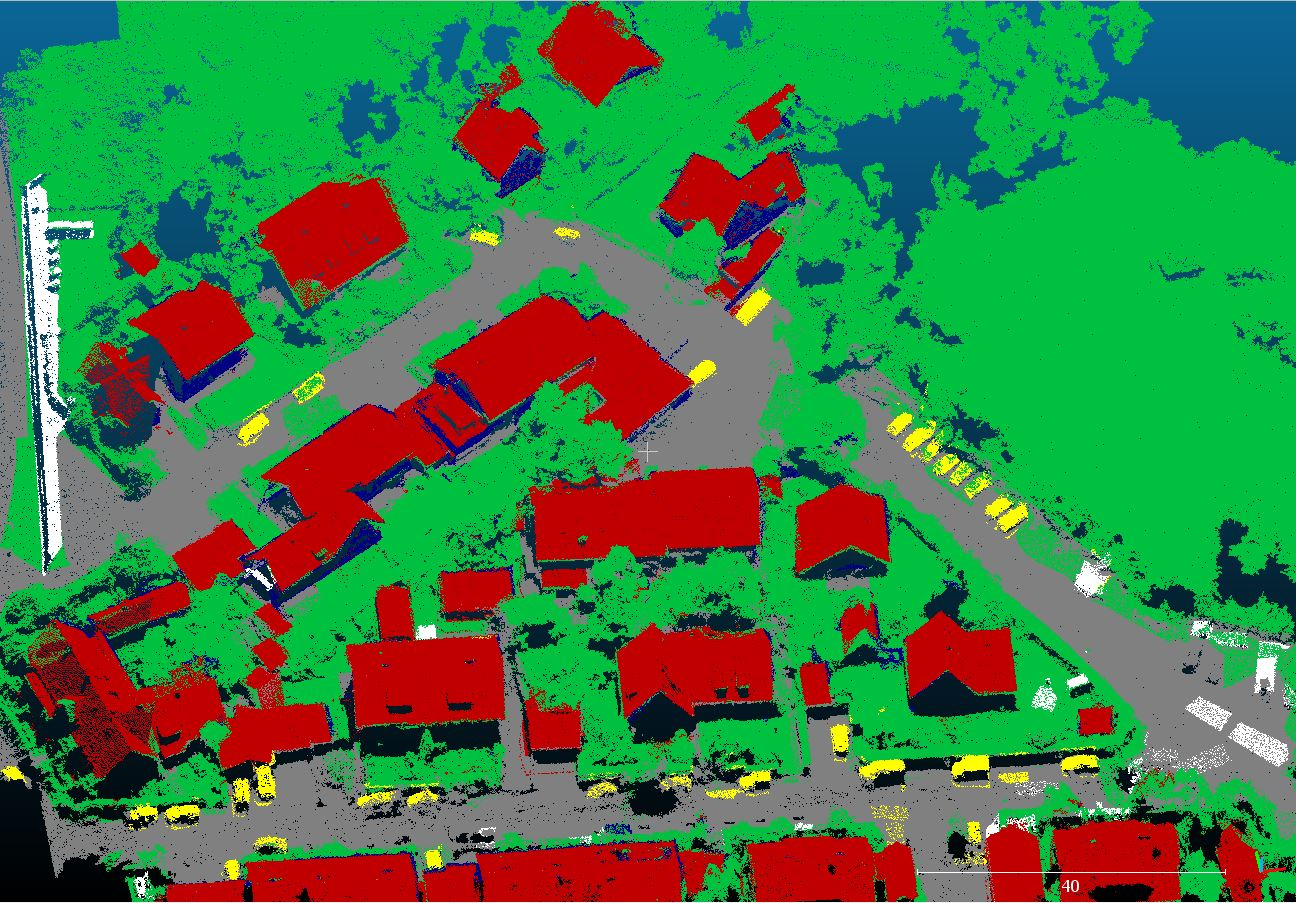
\includegraphics[width=1\linewidth]{fig/eichenau/pc_colored_r.JPG}
  \caption{}

% \end{subfigure}
% \begin{subfigure}{1\columnwidth}
%   \centering
%   
\includegraphics[width=1\linewidth]{fig/colorbar.JPG}

\end{subfigure}
\caption{Annotated UAV point cloud with labels transferred from aerial images. (a) labels transferred from the left-view image, (b) labels transferred from the right-view image}
\label{fig:color_pc}
\end{figure}


It has to be noted that there are slight temporal differences between the two aerial images, therefore a common 3D point in two labeled point clouds may carry different labels. Besides, occlusions and manual labeling mistakes also lead to label inconsistencies between two point clouds. Figure \ref{fig:eichenau_transferred} illustrates a UAV image with labels projected from the two labeled point clouds, where examples of label inconsistencies are highlighted. To tackle this problem, we refine the weak annotation via the proposed Bayesian-CRF model, as described in the following.


\begin{figure}[htb]
 \begin{subfigure}{0.485\columnwidth}
   \centering
\begin{tikzpicture}
    \node[inner sep=0pt] (ima) at (0,0) {\includegraphics[width=1\columnwidth]{fig/eichenau/DSC00826_l.png}};
         \draw[cyan,very thick,rounded corners] (-1.5,0.7) ellipse (0.5 and 0.3);
         \draw[rotate=45,pink,very thick,rounded corners] (0.8,-0.6) ellipse (0.6 and 0.3); 
     %\end{scope}    
 \end{tikzpicture}
   \caption{}  
 \end{subfigure}
~
 \begin{subfigure}{0.485\columnwidth}
   \centering
 \begin{tikzpicture}
\node[inner sep=0pt] (imb) at (0.5\columnwidth,0) {\includegraphics[width=1\columnwidth]{fig/eichenau/DSC00826_r.png}};
     \begin{scope}[xshift=0.5\columnwidth]
         \draw[cyan,very thick,rounded corners] (-1.5,0.7) ellipse (0.5 and 0.3);    
         \draw[rotate=45,pink,very thick,rounded corners] (0.8,-0.6) ellipse (0.6 and 0.3);
     \end{scope}       
\end{tikzpicture}
   \caption{}  
 \end{subfigure}
 
% \begin{subfigure}{0.48\columnwidth}
%   \centering
%   \includegraphics[width=1\linewidth]{fig/DSC00826_l.png}
%   \centerline{(a) }  
% \end{subfigure}
% \begin{subfigure}{0.48\columnwidth}
%   \centering
%   \includegraphics[width=1\linewidth]{fig/DSC00826_r.png}
%   \centerline{(b) }
% \end{subfigure}
\caption{A UAV image with labels transferred from two-view aerial images. (a) labels transferred from left-view aerial image, (b) labels transferred from right-view aerial image. Highlighted areas indicate label inconsistency.}
\label{fig:eichenau_transferred}
\end{figure}


\subsection{Inference}
\subsubsection{3D Point Unary Potentials}The 3D point unary potentials can be derived from either a hard manual labeling or a probability distribution computed by a pixel-wise classifier such as MRF or the softmax function of a CNN. In our case, we obtain the unary potential of each 3D point from the labeling of the point cloud. 

More formally, let $\mathbf{P}$ denote the set of non-occluded 3D points in the input UAV point cloud and $s_i$ denote the label assigned to each point $i\in \mathbf{P}$. The domain of each variable $s_i$ is a set of labels $\mathcal{L} = \{l_1, \dots, l_K\}$, where $K$ denotes the number of classes. In our case, $K = 6, \mathcal{L} = $\big\{\textit{Building}, \textit{Roof}, \textit{Ground}, \textit{Vegetation}, \textit{Car} and \textit{Clutter}\big\}. 

% We project all non-occluded points of the point cloud into a labeled aerial image,the label of each 3D point $s_i$ is encouraged to be the same as the label of the corresponding image pixel $l_0$. In view of the errors of manual labeling and the misalignment between aerial imagery and UAV point cloud, we describe the accuracy of the transferred labels with a subjective possibility $p$, which is set to 0.8 in our experiment. Then the probability of a 3D point $i$ ($i\in \mathbf{P}$) taking the label $s_i$ is: 
% \begin{equation}
% \label{eq:5}
% P\left(s_i\right)=\left\{
% \begin{array}{lcl}
% p & & {s_i = l_0}\\
% \frac{\left(1-p\right)}{n-1} & & {s_i \neq l_0}
% \end{array} \right.
% \end{equation}

% More specifically, let $\mathbf{S}$ denote the set of 3D points in the UAV point cloud and $\mathbf{L^N}$ denote the set of $N$ labels, i.e., \big\{\textit{Building}, \textit{Roof}, \textit{Ground}, \textit{Low vegetation} and \textit{Car}\big\} in our case. Meanwhile, let $l_s$ denote the semantic labeling of the point $s$ from the labeled point cloud with the confidence probability $p$. Assume the labels are propagated from aerial image $k$, $\psi_u^k\left(s_l\right)$ encodes the likelihood of a 3D point $s$ ($s\in \mathbf{S}$) taking the label $l \left(l \in \mathbf{L^N}\right)$, which is defined as:

% \begin{equation}
% \label{eq:5}
% \psi_u\left(s_l\right)=\left\{
% \begin{array}{lcl}
% p & & {l = l_s}\\
% \frac{\left(1-p\right)}{N-1} & & {l \neq l_s}
% \end{array} \right.
% \end{equation}

It needs to be noted that the labeling of UAV point cloud can be transferred from multiple labeled aerial images. Assume we project all non-occluded points of the point cloud into $n$ (in our settings $n = 2$) annotated aerial images to transfer labels, each 3D point is therefore assigned with $n$ sets of labels and the corresponding prior label assignment probabilities are denoted by $P\left(s_i^1\right), \dots, P\left(s_i^n\right)$. In order to combine the information from multiple views, we fuse the potentials by taking the average value

\begin{equation}
\label{eq:6}
P\left(s_i\right)=\frac{\sum_{j=1}^{n}P\left(s_i^j\right)}{n}
\end{equation}

\subsubsection{Pixel Unary Potentials}Pixel unary potential encodes the probability of a image pixel $i$ taking label $x_i$. Based on the assumption that image pixels should carry the same labels with corresponding points in 3D space, we project all the labeled 3D points of the UAV point cloud into UAV images to transfer the labels of 3D points to corresponding image pixels. Since our 3D point cloud is generated via interpolation and has higher spatial resolution than UAV image, each pixel in the UAV image corresponds to multiple 3D points which may carry different labels. For a pixel $i$ on the UAV image, Let \big\{$P\left(s_1\right), \dots, P\left(s_m\right)$\big\} denote the set of the prior probabilities of corresponding 3D points, where $m$ denote the number of 3D points which are projected onto this pixel. The prior probability of a image pixel $i$ taking label $x_i$ is assigned the average a priori of corresponding 3D points, i.e., 
\begin{equation}
\label{eq:7}
P\left(x_i\right)=\frac{\sum_{j=1}^{m}P\left(s_j\right)}{m}
\end{equation}
Where, $P\left(x_i\right)$ is namely the prior belief in Equation \ref{eq:3}.


Given additional evidence, the label assignment probabilities are then updated using the Bayesian rule. In this experiment, we exploited the geometric information, i.e., the relative height above the ground, which was obtained by ground filtering using the Top-hat algorithm \cite{Mongus2012tophat}. The likelihood of observation on height for given class, denoted by $P\left(H \mid \mathbf{x}\right)$ ($H$ is namely an instance of $\mathbf{O}$ in Equation \ref{eq:3}), is empirically estimated based on image statistics. Since height is continuous, $P\left(H \mid \mathbf{x}\right)$ is specified as the probability density function of $H$ for given class. In our settings, we model the probability density function as a normal distribution. In complicated cases, e.g., \textit{Vegetation} include trees and grassland which have different distribution on height, we then model the likelihood function as a weighted sum of normal distributions, i.e., $f(H;\mu ,\sigma ^{2}) = \sum \omega_i\frac {1}{\sqrt {2\pi \sigma_i ^{2}}}e^{-\frac {(H-\mu_i )^{2}}{2\sigma_i ^{2}}}$. A visualization of the likelihood functions is illustrated in Figure \ref{fig:ei_distrib}, and the parameter settings are listed in Table \ref{tab:ei_para_h}. Besides, considering \textit{roof} is generally higher than 2 meters, we set its lower bound of height as 2m; since \textit{building} (facades) has no height measurements on the heightmap, their prior labeling probabilities were not updated via Bayesian inference. The hyperparameters (e.g., $\omega, \mu ,\sigma$) for the probability density functions were manually tuned in the experiment. According to our experience, the performance of inference is not sensitive to the parameter setting as long as they reasonably describe the reality.  

\begin{figure}[htb]
    \centering
       \begin{subfigure}{0.95\columnwidth}
	       \centering
           \includegraphics[width=\linewidth]{fig/eichenau/ei_height}	
       \end{subfigure}      
       \caption{Probability distribution of height for \textbf{Area 1}.}
       \label{fig:ei_distrib}
\end{figure}

\begin{table}[htbp]
  \centering
  \caption{Parameter settings of probability distribution functions for height, Eichenau Dataset.}
    \begin{tabular}{c|c|c|c|c|c|c}
    \hline
    \textbf{Parameter} & \textbf{Ground} & \textbf{Roof} & \textbf{Car}  & \textbf{Clutter} & \multicolumn{2}{c}{\textbf{Vegetation}} \\
    %Define if appropriate
          
    \hline
    $\omega$     & 2     & 1     & 1     & 0.5  &1  & 0.5\\
    
    $\mu$     & 0     & 7   & 1.3     & 0.5  &3  & 7\\
    
    $\sigma$ & 0.5   & 3  & 0.6     & 0.5  &1  & 3\\
    \hline
    \end{tabular}%
  \label{tab:ei_para_h}%
\end{table}%

\subsubsection{Inference}We performed inference of the CRF model based on the implementation\footnote{https://github.com/lucasb-eyer/pydensecrf} of \cite{crf2012}. In Figure \ref{fig:ei_inference}, column (a) depicts a few examples of automatically generated annotations while column (b) shows corresponding manually labeled annotations. It can be seen that the inferred annotations have high semantic accuracy and conform well to the image gradients at class boundaries, outperforming the manual labeling especially for objects with irregular shapes such as trees. 

There are also a few errors in the inferred annotations, which are caused by three major factors: 1. low contrast in dark or shaded areas; 2. strong gradient at shadow boarders; 3. wrong height value (especially for moving cars). Therefore it is recommended to apply the proposed method for annotating static objects on shadow-free images.

\begin{figure}[htb]
\begin{subfigure}{0.49\columnwidth}
  \centering
  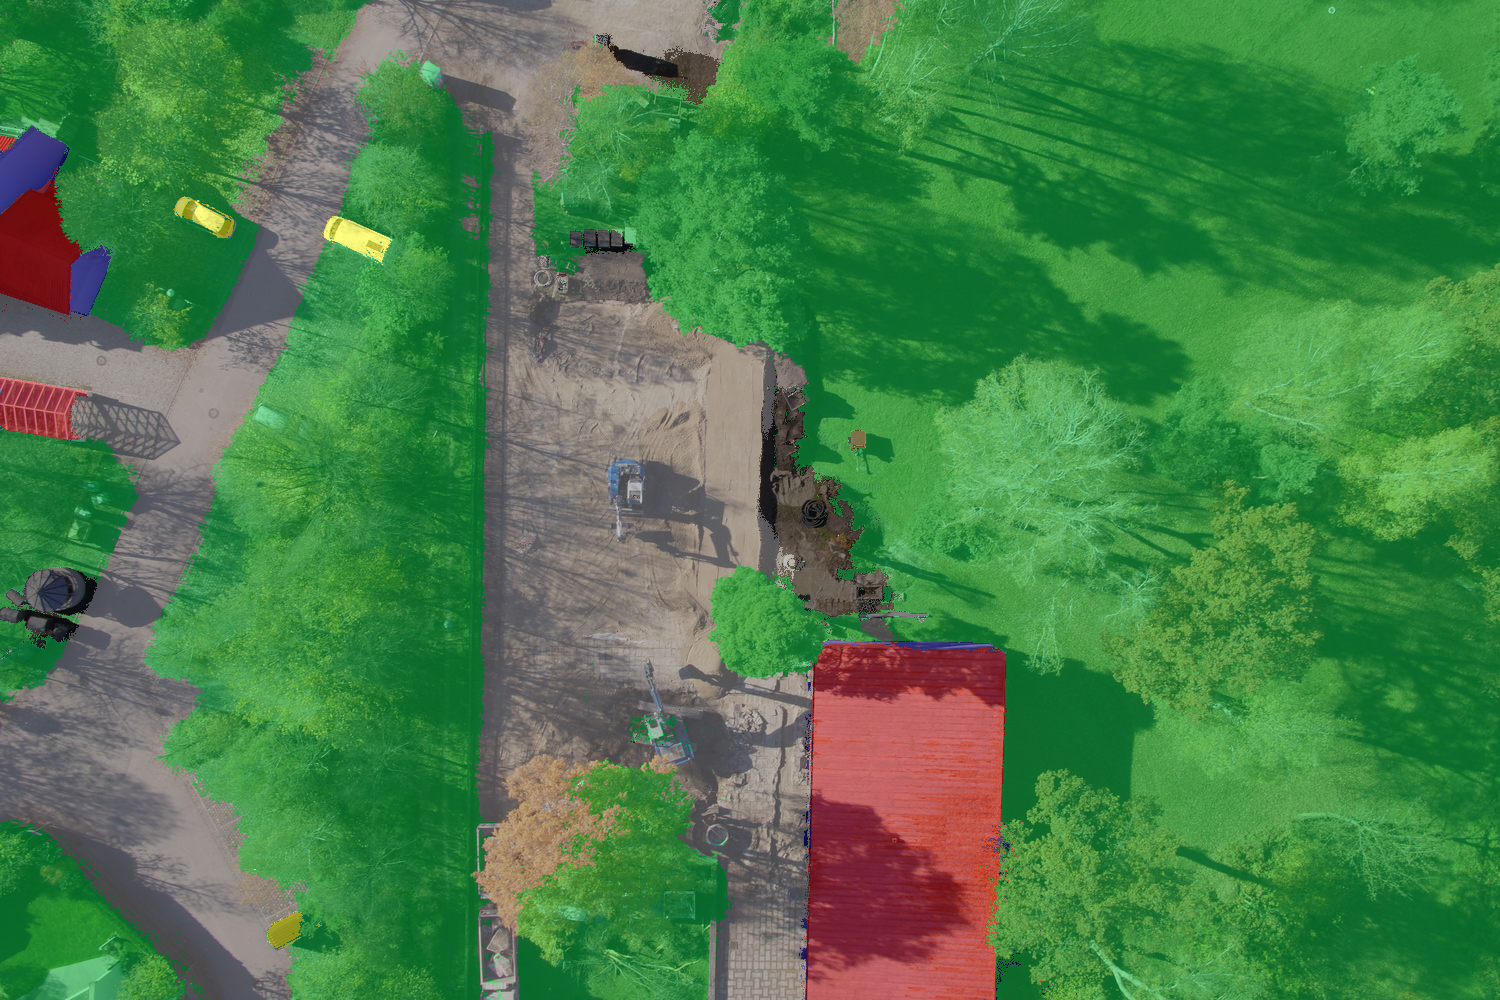
\includegraphics[width=1\linewidth]{fig/overlay/DSC00798_auto_lay.png}
  \label{fig:sfig1}
\end{subfigure}\hfill
\vspace{-0.35\baselineskip}
\begin{subfigure}{0.49\columnwidth}
  \centering
  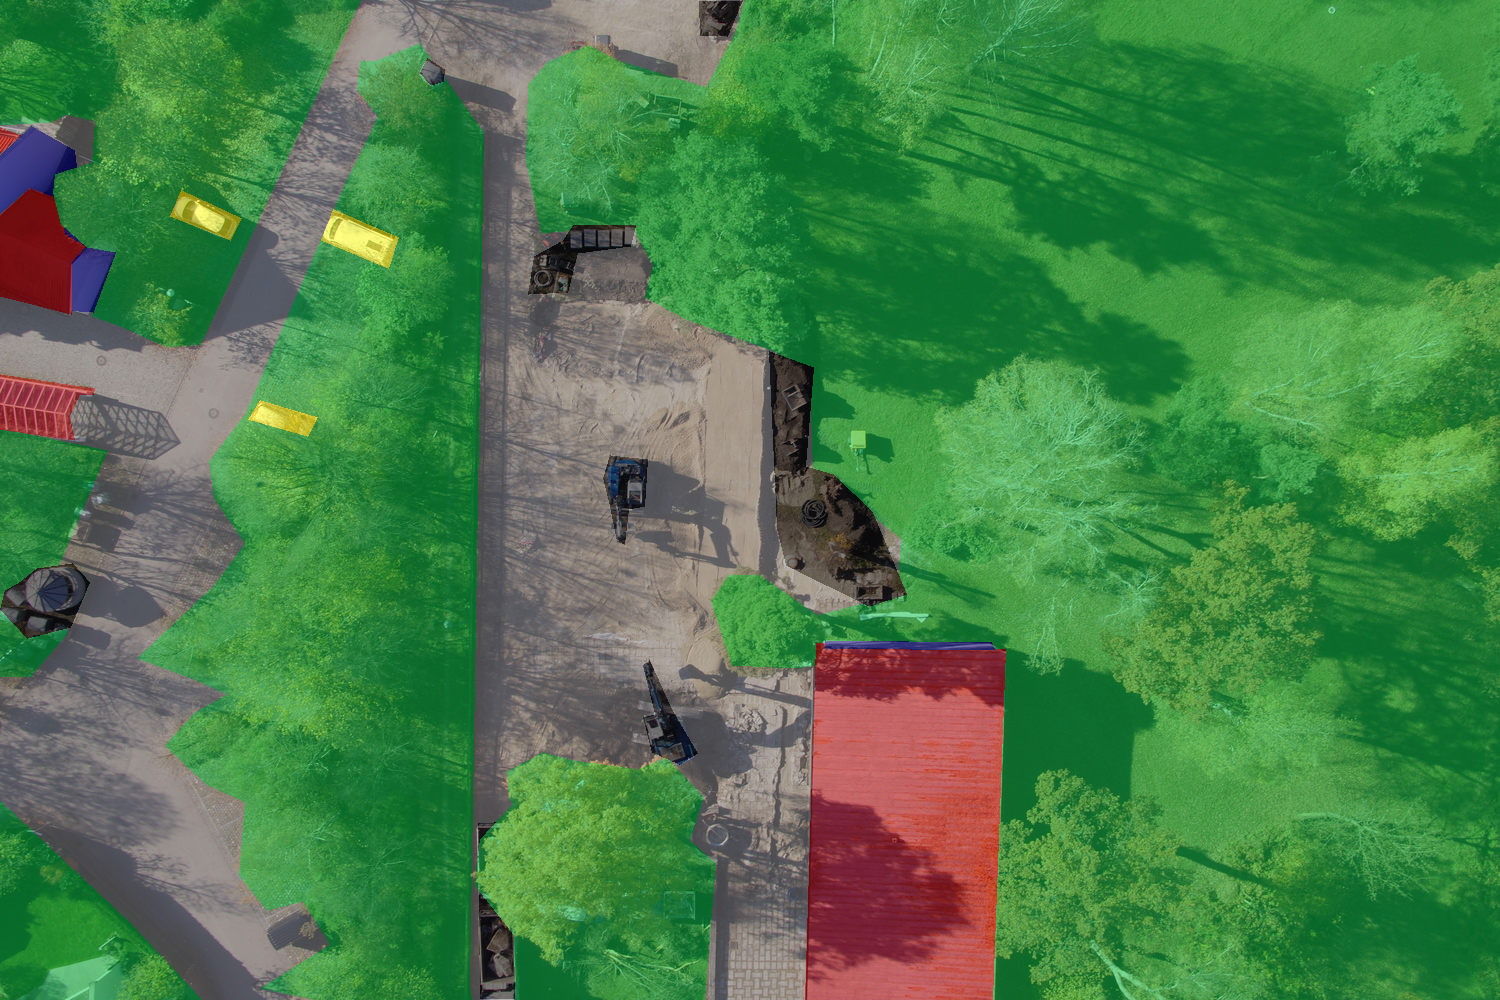
\includegraphics[width=1\linewidth]{fig/overlay/DSC00798_manual_lay.png}
  \label{fig:sfig1}
\end{subfigure}
\vspace{-0.35\baselineskip}

% \begin{subfigure}{0.49\columnwidth}
%   \centering
%   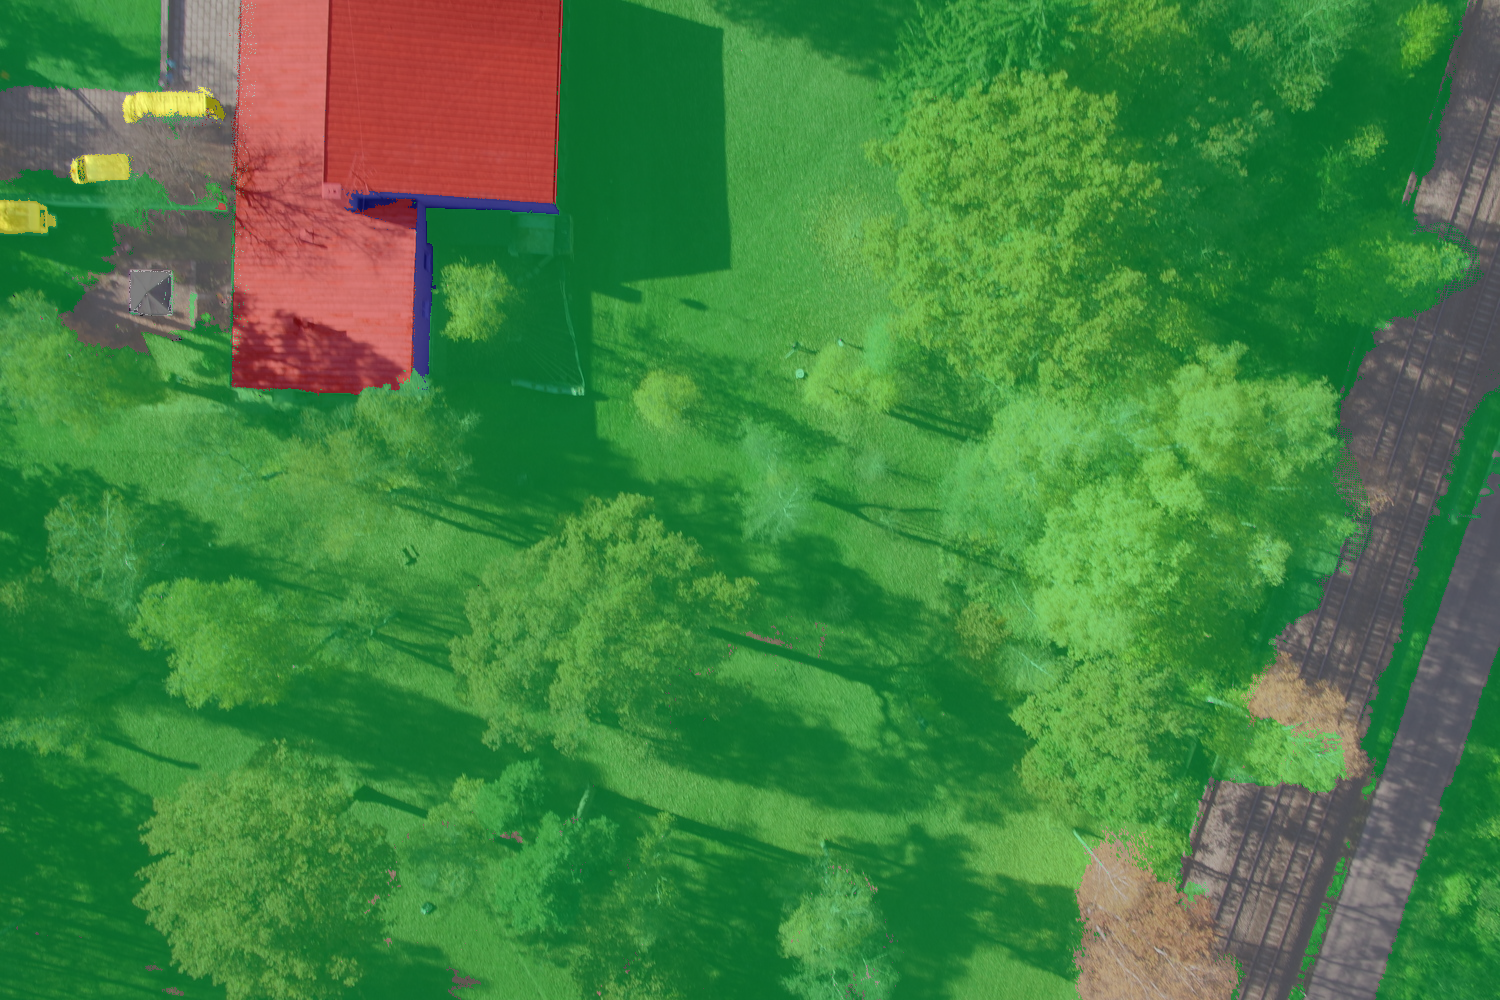
\includegraphics[width=1\linewidth]{fig/overlay/DSC00809_auto_lay.png}
%   \label{fig:sfig1}
% \end{subfigure}\hfill
% \begin{subfigure}{0.49\columnwidth}
%   \centering
%   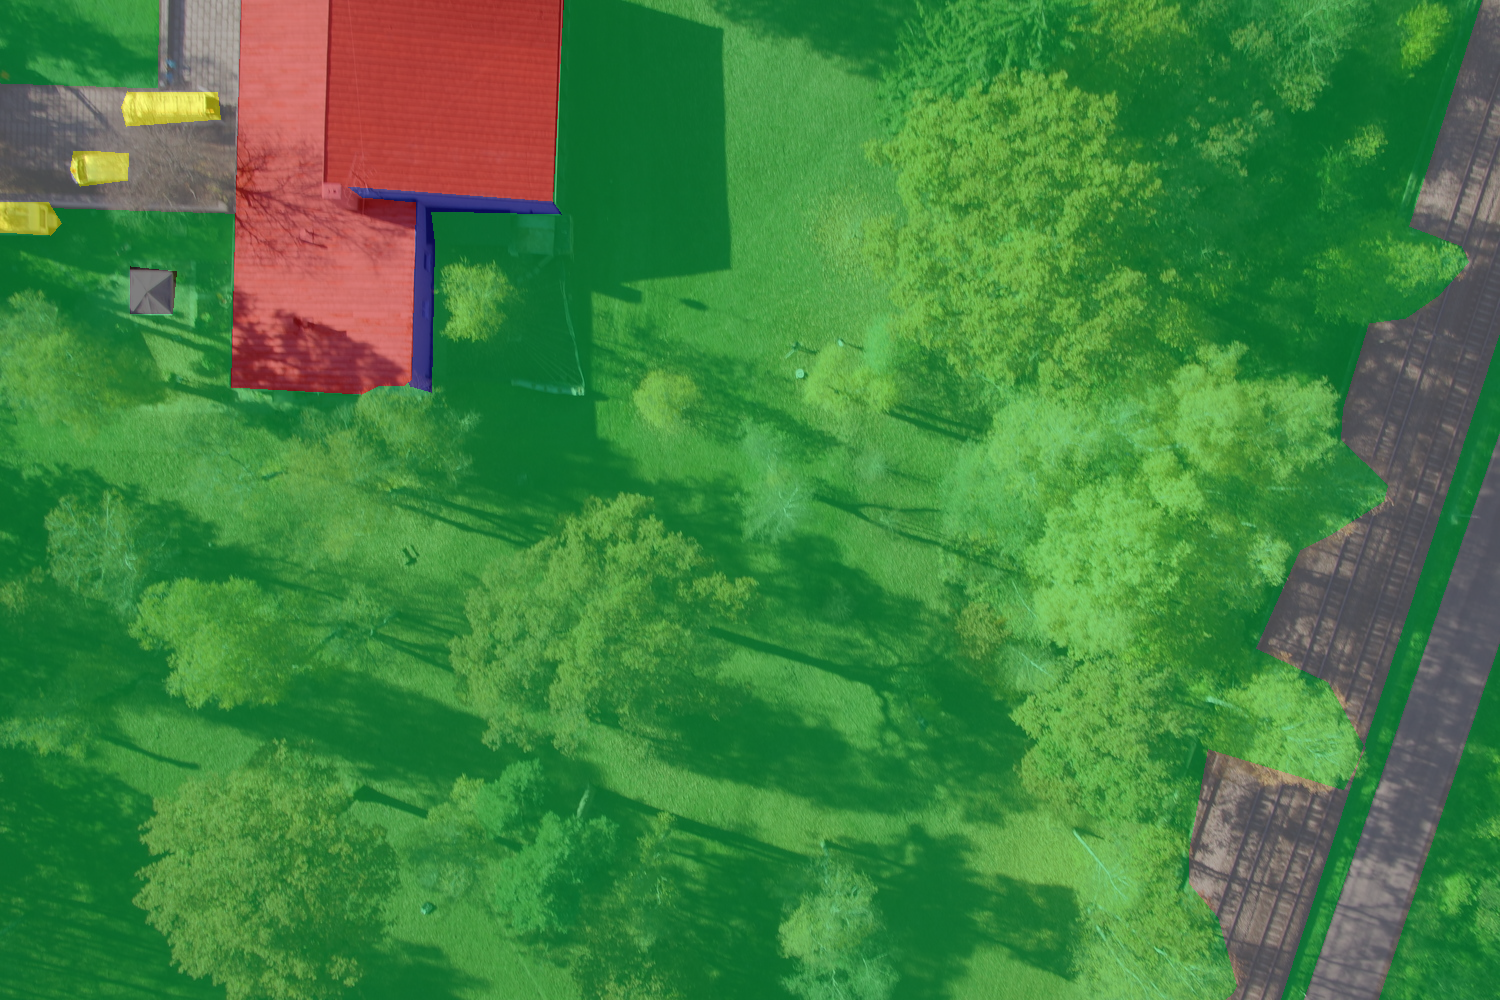
\includegraphics[width=1\linewidth]{fig/overlay/DSC00809_manual_lay.png}
%   \label{fig:sfig1}
% \end{subfigure}
% \vspace{-0.5\baselineskip}

% \begin{subfigure}{0.49\columnwidth}
%   \centering
%   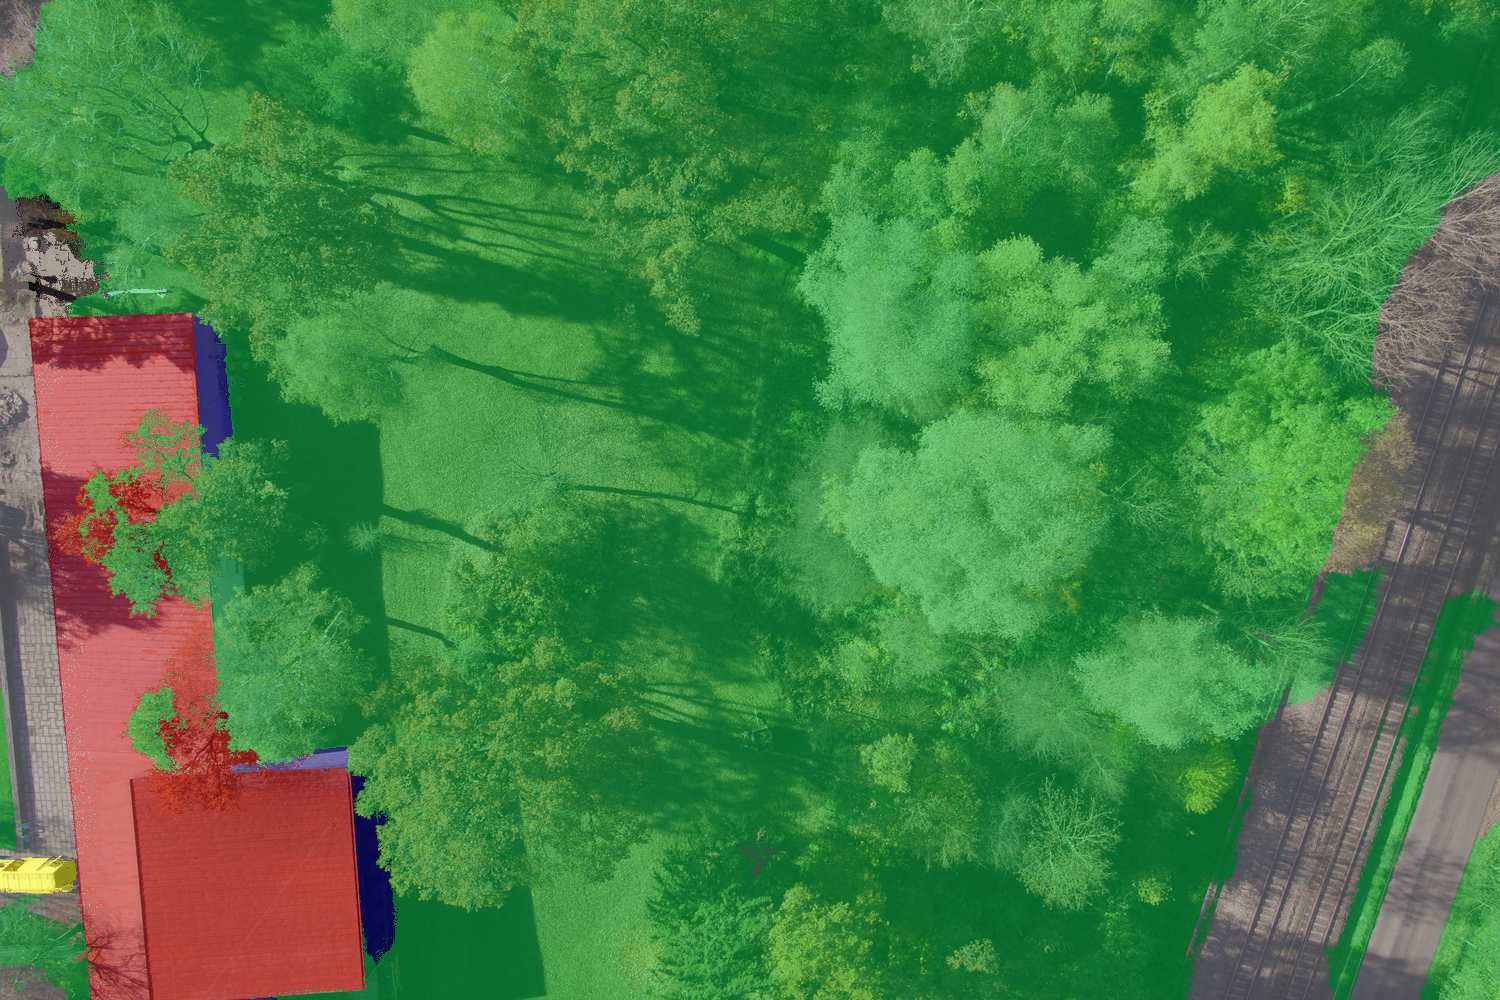
\includegraphics[width=1\linewidth]{fig/overlay/DSC00818_auto_lay.png}
%   \label{fig:sfig1}
% \end{subfigure}\hfill
% \begin{subfigure}{0.49\columnwidth}
%   \centering
%   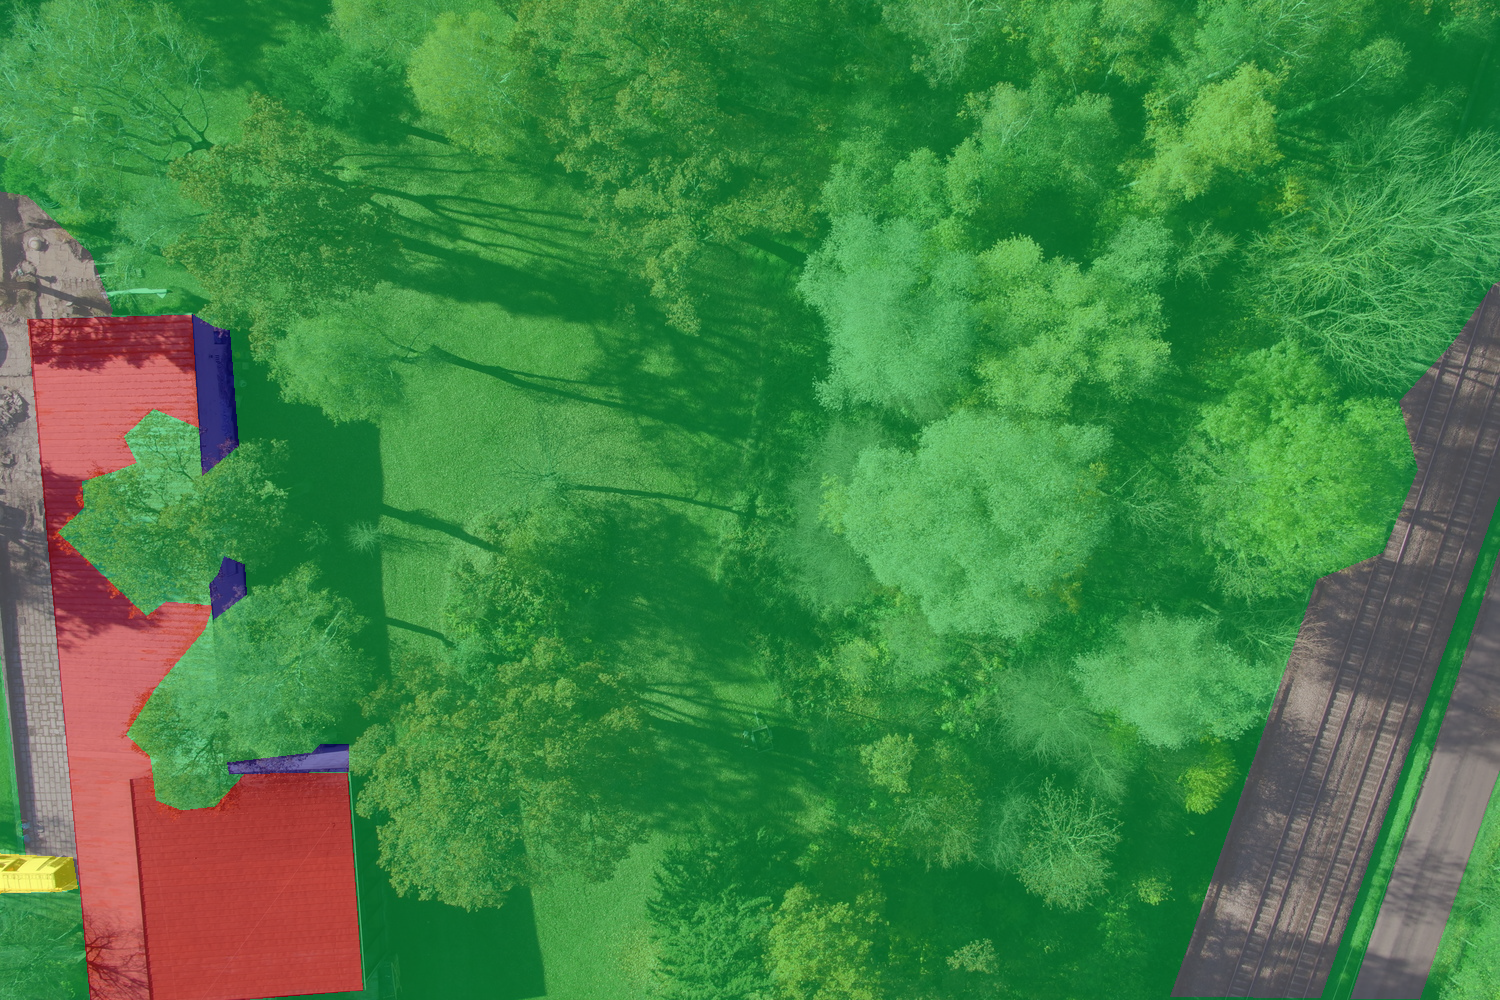
\includegraphics[width=1\linewidth]{fig/overlay/DSC00818_manual_lay.png}
%   \label{fig:sfig1}
% \end{subfigure}
% \vspace{-0.5\baselineskip}

% \begin{subfigure}{0.49\columnwidth}
%   \centering
%   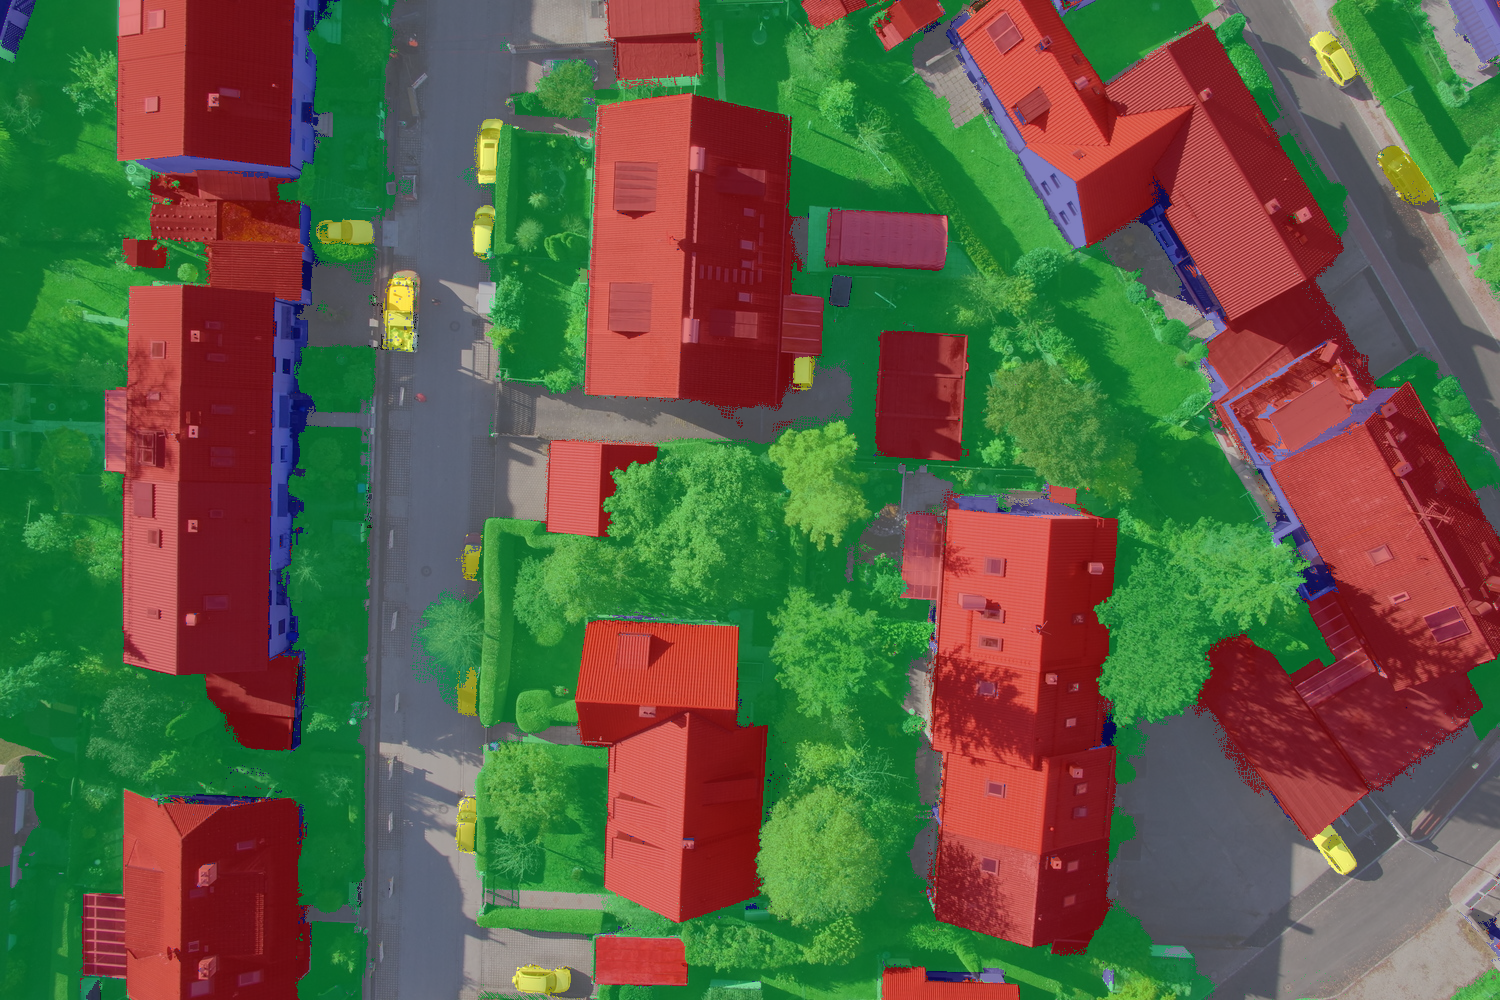
\includegraphics[width=1\linewidth]{fig/overlay/DSC00830_auto_lay.png}
%   \label{fig:sfig1}
% \end{subfigure}\hfill
% \vspace{-0.35\baselineskip}
% \begin{subfigure}{0.49\columnwidth}
%   \centering
%   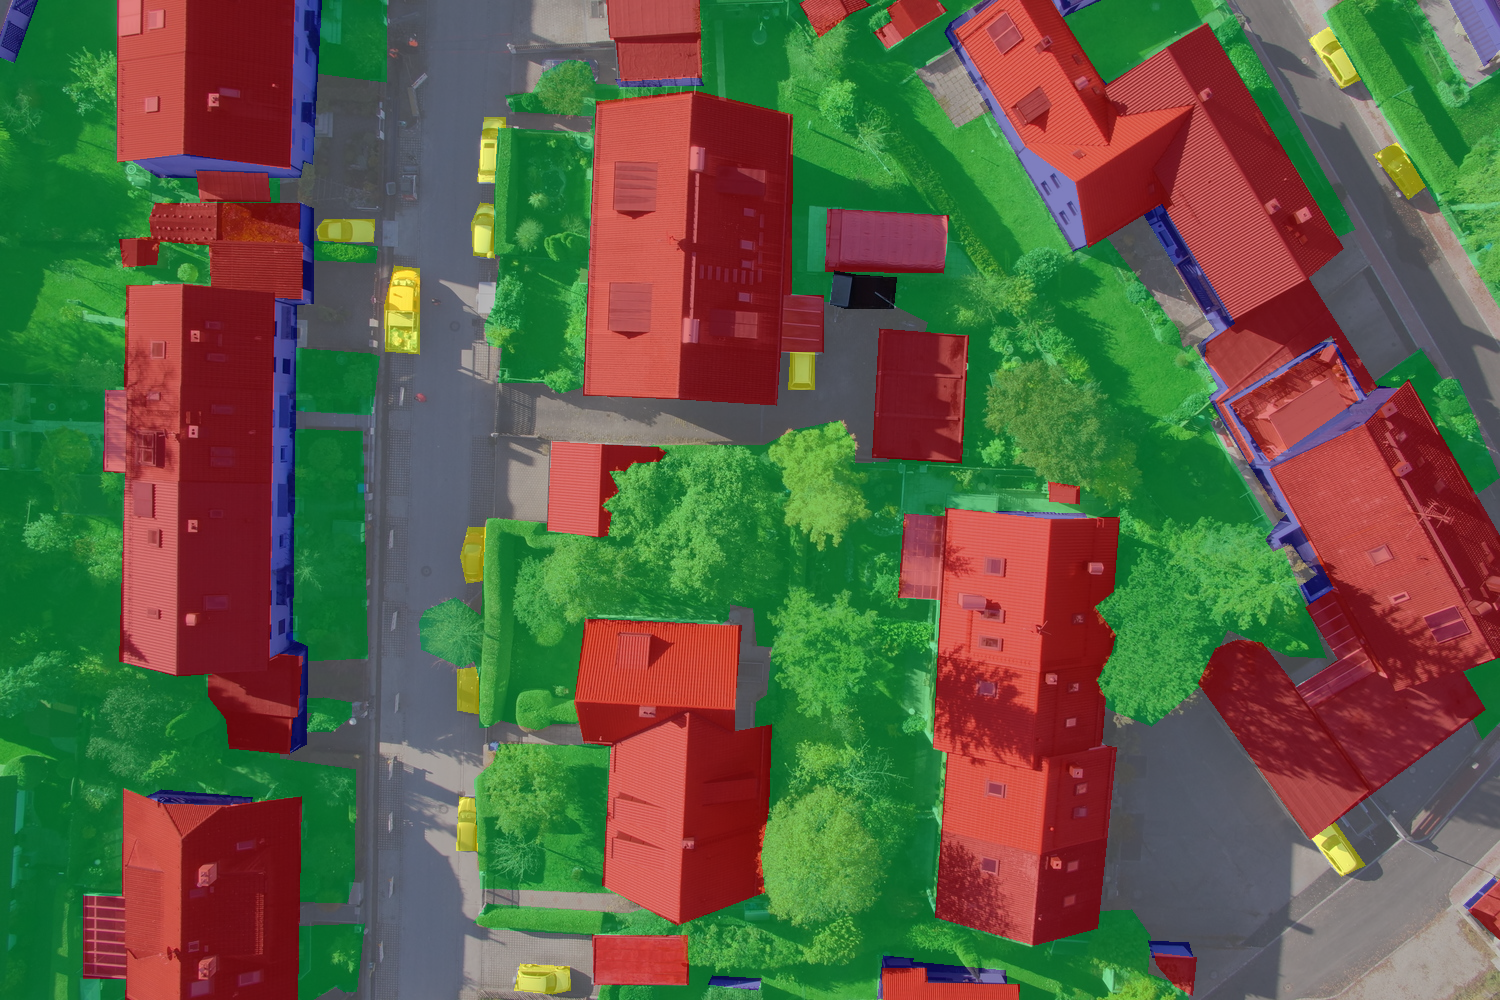
\includegraphics[width=1\linewidth]{fig/overlay/DSC00830_manual_lay.png}
%   \label{fig:sfig1}
% \end{subfigure}
% \vspace{-0.35\baselineskip}

\begin{subfigure}{0.49\columnwidth}
  \centering
  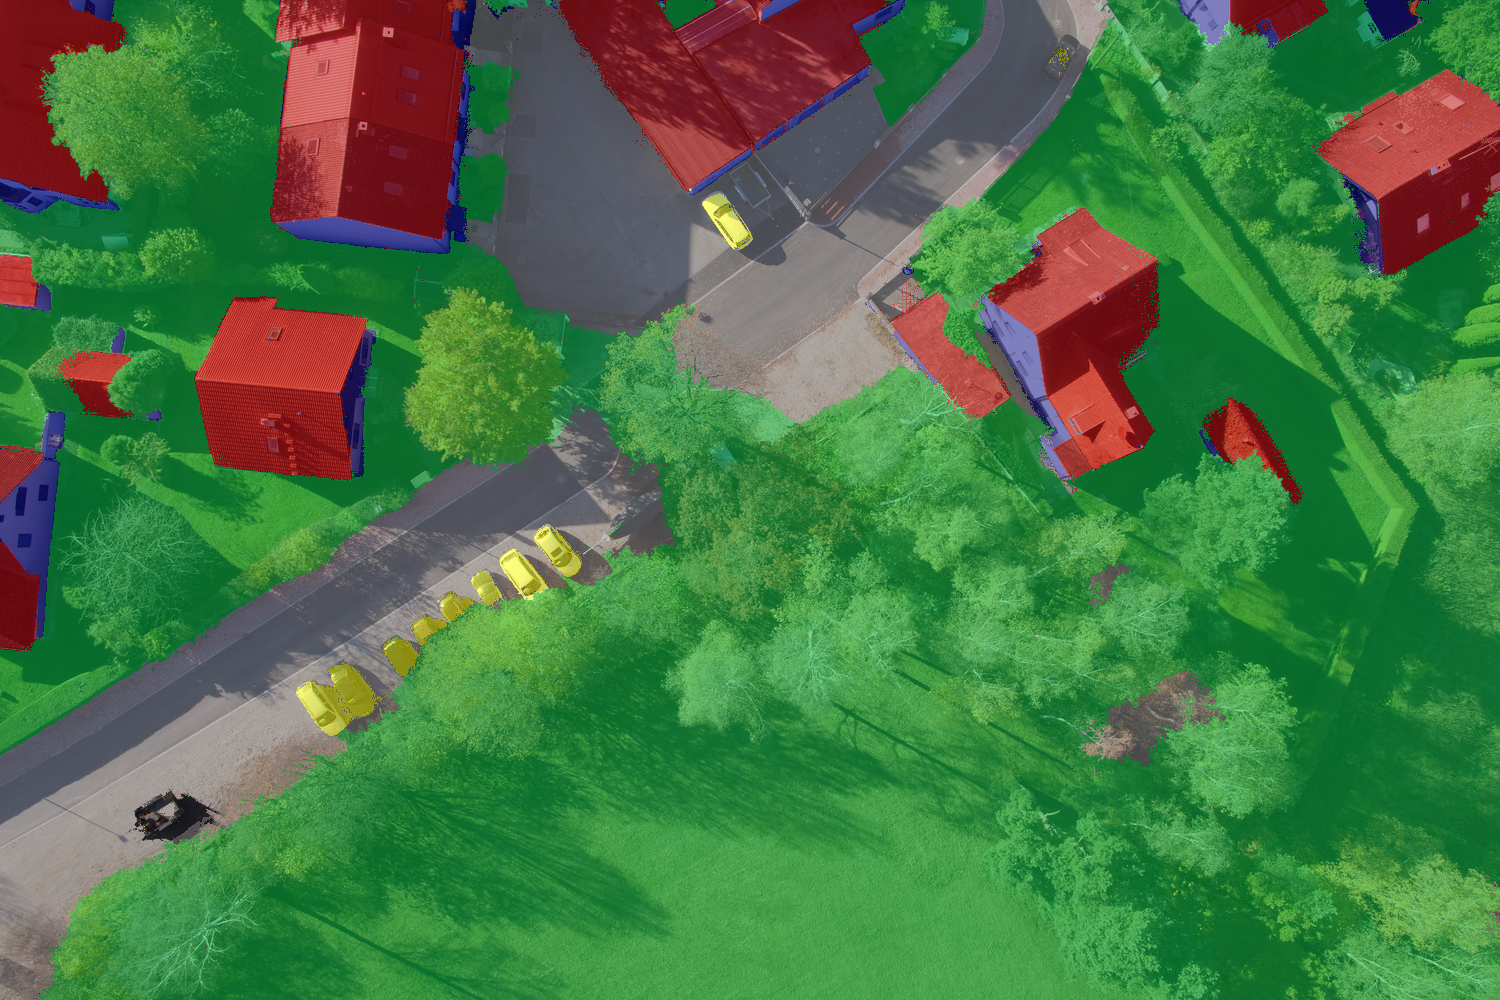
\includegraphics[width=1\linewidth]{fig/overlay/DSC00847_auto_lay.png}
  \label{fig:sfig1}
\end{subfigure}\hfill
\vspace{-0.35\baselineskip}
\begin{subfigure}{0.49\columnwidth}
  \centering
  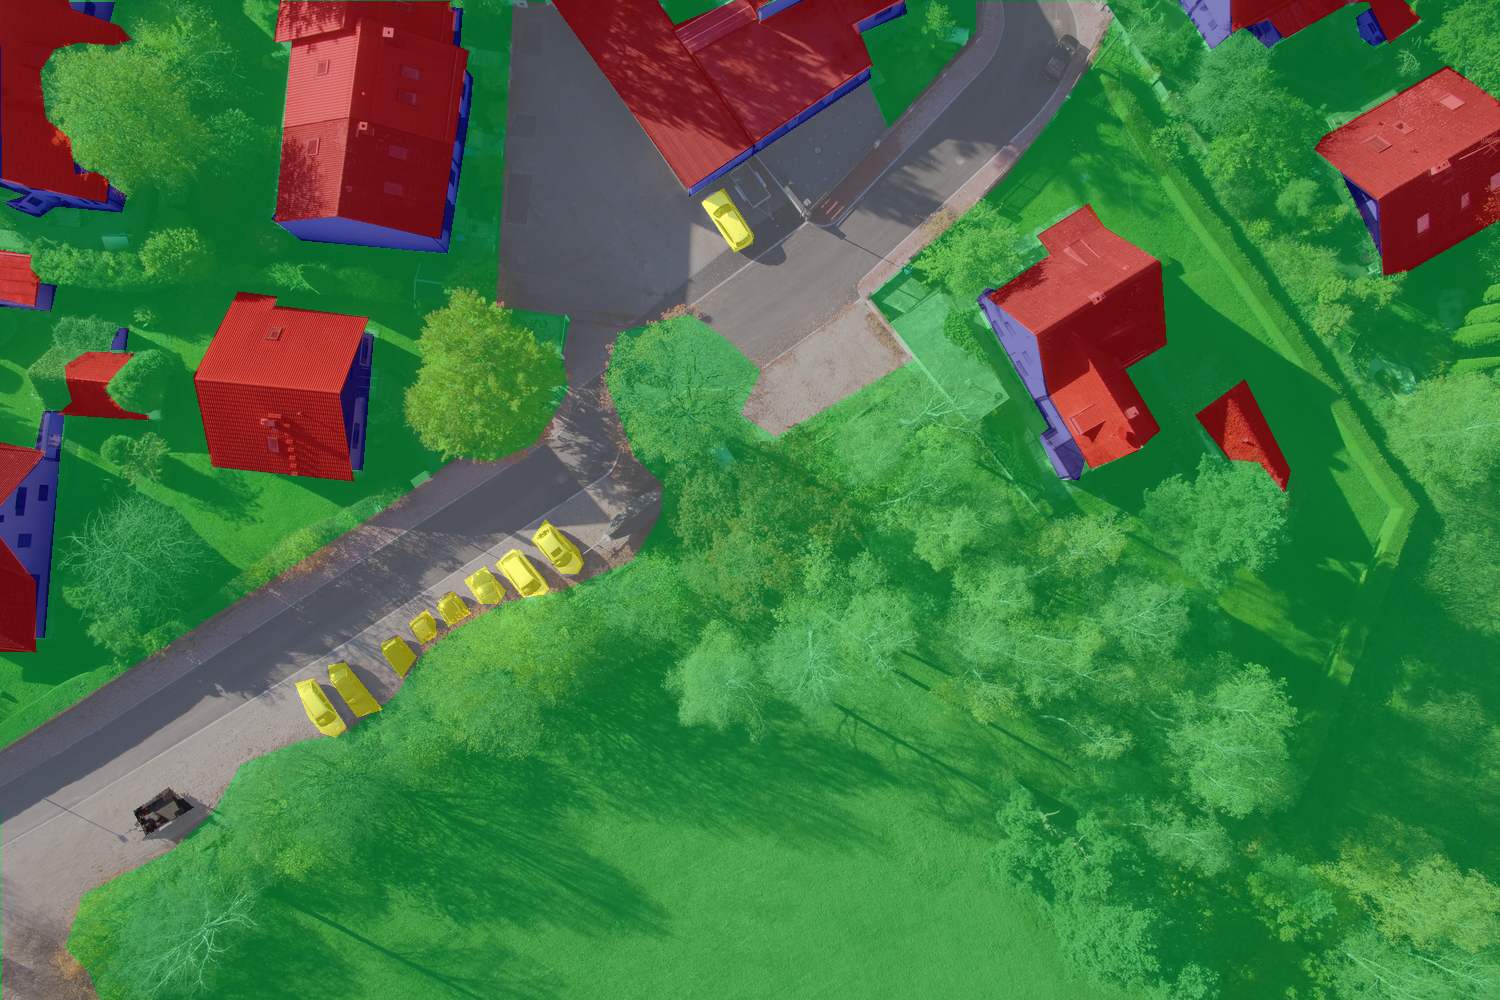
\includegraphics[width=1\linewidth]{fig/overlay/DSC00847_manual_lay.png}
  \label{fig:sfig1}
\end{subfigure}
\vspace{-0.35\baselineskip}

\begin{subfigure}{0.49\columnwidth}
  \centering
  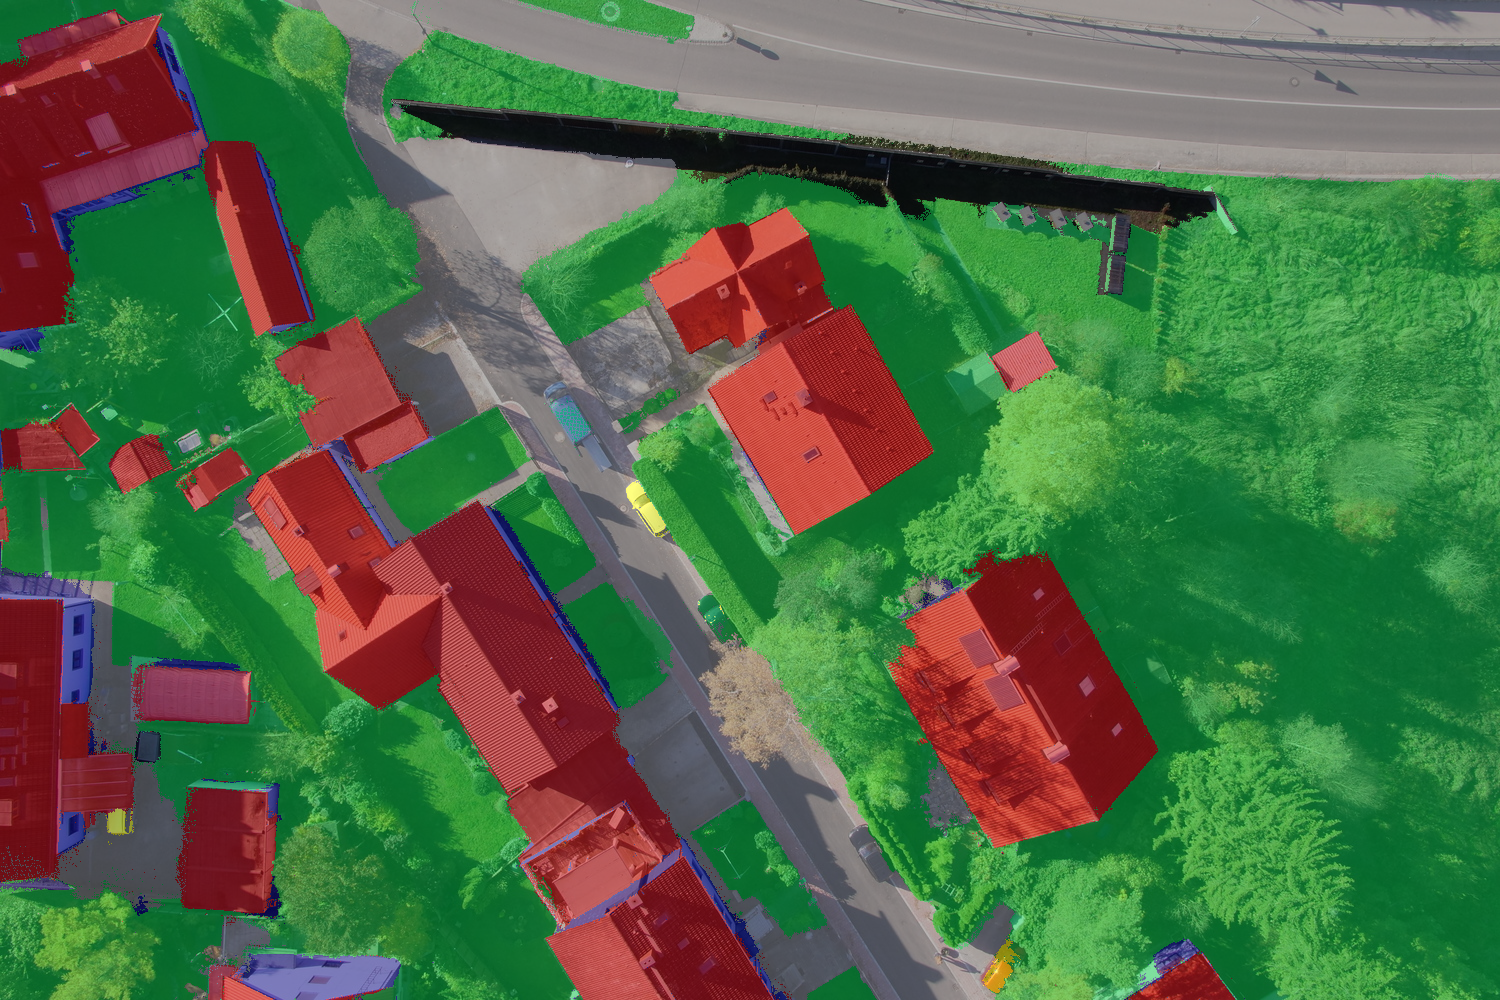
\includegraphics[width=1\linewidth]{fig/overlay/DSC00852_auto_lay.png}
\vspace{-0.35\baselineskip}
  \label{fig:sfig1}
  \caption{}
\end{subfigure}\hfill
\begin{subfigure}{0.49\columnwidth}
  \centering
  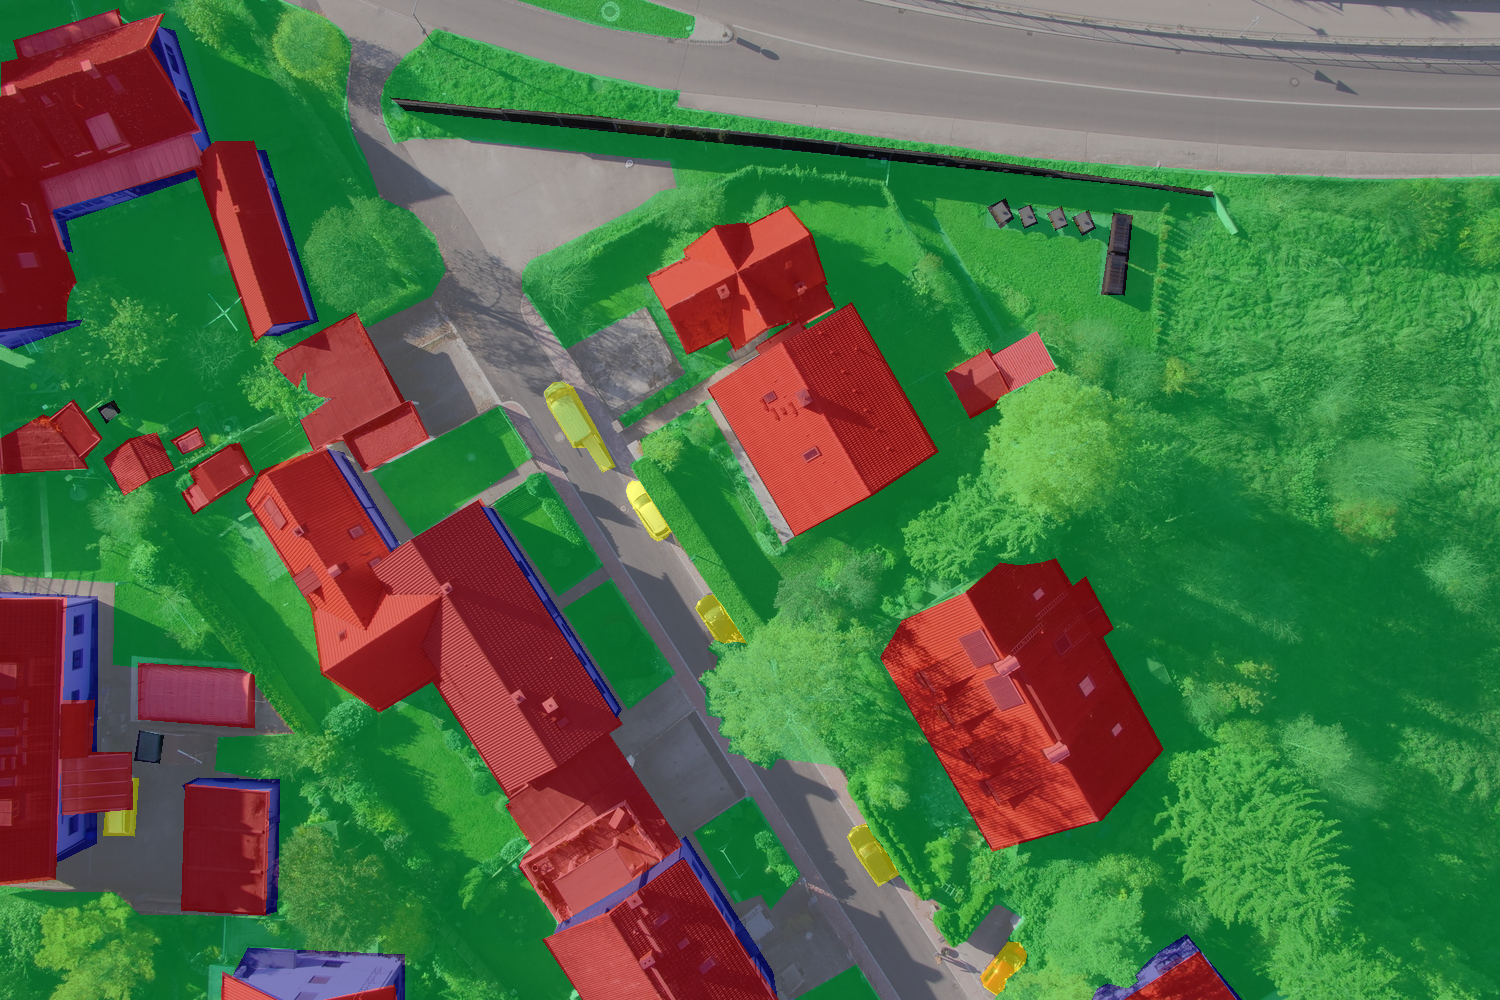
\includegraphics[width=1\linewidth]{fig/overlay/DSC00852_manual_lay.png}
\vspace{-0.35\baselineskip}
  \label{fig:sfig1}
  \caption{}
\end{subfigure}

\caption{Comparison of inferred image annotations (a) and manual annotations (b) overlaying on original UAV images.}
\label{fig:ei_inference}
\end{figure}

% \begin{figure}[h]
% \begin{minipage}[b]{0.32\linewidth}
%   \centering
%   \centerline{\epsfig{figure=fig/DSC00835.png,width=2.4cm}}
%   \centerline{(a)}
% \end{minipage}
% \hfill
% \begin{minipage}[b]{0.32\linewidth}
%   \centering
%   \centerline{\epsfig{figure=fig/DSC00835.JPG,width=2.4cm}}
%   \centerline{(b)}
% \end{minipage}
% \hfill
% \begin{minipage}[b]{0.32\linewidth}
%   \centering
%   \centerline{\epsfig{figure=fig/DSC00835_anno.png,width=2.4cm}}
%   \centerline{(c) }
% \end{minipage}
% \caption{Comparison of transferred annotations with manual annotations. (a) is automatic annotation and (c) is manual annotation, (b) is corresponding UAV image}
% \label{fig:eichenau_anno}
% \end{figure}


\subsection{Training a CNN Using Generated Annotations}
\label{sec:seg}

In order to validate the utility of the automatically generated annotations, we deployed them as ground-truth data to train a fully convolutional network (FCN) \cite{fcn} for image semantic segmentation, and compared the performance with the segmentation using manual annotations. To be specific, we selected 28 UAV images featuring different regions of the scene and manually labeled them as ground-truth data, which are then split into 23 training samples and 5 testing samples. In parallel, we applied the proposed method to annotate the 23 images as pseudo ground-truth data for training. Both sets of training data are augmented via cropping and rotating, resulting in 8208 images with the size of 300$\times$300 pixels.

% The learning procedure is implemented under the deep learning framework Caffe. We fined tune the FCN-8s model \cite{fcn} \footnote{https://github.com/shelhamer/fcn.berkeleyvision.org} with our dataset. Besides, we plug in the CRF-RNN \cite{crfasrnn_ICCV2015} \footnote{https://github.com/torrvision/crfasrnn} layer in order to achieve sharp edges at class borders.  The corresponding training loss is shown in Figure \ref{fig:loss_ei}. 
% \begin{figure}[htb]
%     \centering
%        \begin{subfigure}[b]{0.4\columnwidth}
% 	       \centering
% 			% This file was created by matlab2tikz.
%
%The latest updates can be retrieved from
%  http://www.mathworks.com/matlabcentral/fileexchange/22022-matlab2tikz-matlab2tikz
%where you can also make suggestions and rate matlab2tikz.
%
\definecolor{mycolor1}{rgb}{0.00000,0.44700,0.74100}%

\begin{tikzpicture}[trim axis left, trim axis right]

\begin{axis}[%
width=0.8\linewidth,
height=.1\textheight,
scale only axis,
%grid = major,
xlabel style={font=\color{white!15!black}},
xlabel={Iterations},
ylabel style={font=\color{white!15!black}},
ylabel={Training loss},
ylabel near ticks,
label style={font=\small},
tick label style={font=\small},
xmin=0,
xmax=6000,
ymin=0,
ymax=2,
axis background/.style={fill=white},
axis x line*=bottom,
axis y line*=left
]
\addplot [color=mycolor1, forget plot]
  table{%
0	1.94591	//
20	0.757956	//
40	1.89001	//
60	1.54026	//
80	1.31852	//
100	0.478372	//
120	0.907423	//
140	0.506405	//
160	0.975745	//
180	0.761873	//
200	0.0471938	//
220	1.15339	//
240	1.19461	//
260	0.0406444	//
280	0.848949	//
300	0.694436	//
320	0.537948	//
340	0.417714	//
360	0.0107367	//
380	0.217752	//
400	0.528378	//
420	0.0738107	//
440	0.876134	//
460	0.267503	//
480	0.446599	//
500	0.412888	//
520	0.996446	//
540	1.00779	//
560	0.0120552	//
580	0.685688	//
600	0.5789	//
620	0.343378	//
640	0.806558	//
660	0.338166	//
680	0.114689	//
700	0.272869	//
720	0.281811	//
740	0.438427	//
760	1.11787	//
780	1.20678	//
800	0.314791	//
820	0.665357	//
840	0.780405	//
860	0.0497408	//
880	1.1158	//
900	0.185025	//
920	0.563275	//
940	0.185735	//
960	0.342823	//
980	0.696456	//
1000	0.687274	//
1020	0.469287	//
1040	0.0587835	//
1060	0.566204	//
1080	1.10192	//
1100	0.445571	//
1120	0.46971	//
1140	1.68777	//
1160	0.409147	//
1180	0.674388	//
1200	0.00308775	//
1220	0.238722	//
1240	0.458255	//
1260	0.104631	//
1280	0.0105018	//
1300	0.406052	//
1320	0.462107	//
1340	0.248619	//
1360	1.49936	//
1380	0.419478	//
1400	0.713174	//
1420	0.666846	//
1440	0.63498	//
1460	1.06531	//
1480	0.983216	//
1500	0.461582	//
1520	0.00370886	//
1540	0.174168	//
1560	1.21256	//
1580	0.831018	//
1600	0.0187168	//
1620	0.166934	//
1640	0.796713	//
1660	0.676476	//
1680	0.757966	//
1700	0.0900782	//
1720	0.910206	//
1740	0.405392	//
1760	0.558163	//
1780	0.300626	//
1800	0.162005	//
1820	0.305551	//
1840	0.589163	//
1860	0.522725	//
1880	0.914599	//
1900	0.176012	//
1920	0.186275	//
1940	0.56452	//
1960	0.736039	//
1980	0.626066	//
2000	0.240372	//
2020	0.882863	//
2040	0.609479	//
2060	0.482813	//
2080	0.535819	//
2100	0.379499	//
2120	0.436505	//
2140	0.325723	//
2160	1.0161	//
2180	0.831443	//
2200	0.159328	//
2220	0.398611	//
2240	0.200511	//
2260	0.480007	//
2280	0.0661878	//
2300	0.195308	//
2320	0.35753	//
2340	0.0431824	//
2360	0.0472414	//
2380	0.462711	//
2400	0.518316	//
2420	0.742494	//
2440	0.903704	//
2460	0.510225	//
2480	0.834799	//
2500	0.116631	//
2520	0.368022	//
2540	0.331938	//
2560	0.637432	//
2580	0.514596	//
2600	0.602165	//
2620	0.0191897	//
2640	0.560895	//
2660	0.543673	//
2680	0.28856	//
2700	0.0123799	//
2720	0.558442	//
2740	0.344259	//
2760	0.670001	//
2780	0.349163	//
2800	0.386303	//
2820	0.380701	//
2840	0.0304586	//
2860	0.625235	//
2880	0.016557	//
2900	0.0276236	//
2920	0.817203	//
2940	0.227191	//
2960	0.224104	//
2980	0.489584	//
3000	0.602426	//
3020	0.395894	//
3040	0.634508	//
3060	0.207874	//
3080	0.482655	//
3100	0.50206	//
3120	0.317508	//
3140	0.362752	//
3160	0.879679	//
3180	0.397803	//
3200	0.447426	//
3220	0.753741	//
3240	0.691965	//
3260	0.374221	//
3280	0.455296	//
3300	0.315058	//
3320	0.536134	//
3340	0.354448	//
3360	0.89244	//
3380	0.201252	//
3400	0.0854065	//
3420	0.425875	//
3440	0.363877	//
3460	0.0142245	//
3480	0.11407	//
3500	0.613095	//
3520	0.625613	//
3540	0.735008	//
3560	0.315089	//
3580	0.30766	//
3600	0.642609	//
3620	0.65781	//
3640	0.177548	//
3660	0.260767	//
3680	0.312976	//
3700	0.184591	//
3720	0.469561	//
3740	0.0523288	//
3760	0.0201491	//
3780	0.142606	//
3800	0.158524	//
3820	0.292735	//
3840	0.0273714	//
3860	0.359143	//
3880	0.319341	//
3900	0.393675	//
3920	0.317747	//
3940	0.496386	//
3960	0.00778279	//
3980	0.572116	//
4000	0.43043	//
4020	0.216011	//
4040	0.675854	//
4060	0.579221	//
4080	0.241387	//
4100	0.253048	//
4120	0.014866	//
4140	0.386391	//
4160	0.286219	//
4180	0.34639	//
4200	0.577207	//
4220	0.0984837	//
4240	0.604977	//
4260	0.0939065	//
4280	0.254868	//
4300	0.00659569	//
4320	0.234503	//
4340	0.659678	//
4360	0.0646358	//
4380	0.148737	//
4400	0.389674	//
4420	0.353381	//
4440	0.484986	//
4460	0.258161	//
4480	0.0140436	//
4500	0.451347	//
4520	0.795989	//
4540	0.406646	//
4560	0.0403323	//
4580	0.0526878	//
4600	0.190371	//
4620	0.39032	//
4640	0.620069	//
4660	0.73698	//
4680	0.118145	//
4700	0.0320273	//
4720	0.364943	//
4740	0.0277352	//
4760	0.024928	//
4780	0.494511	//
4800	0.240821	//
4820	0.351838	//
4840	0.0727765	//
4860	0.288887	//
4880	0.0186373	//
4900	0.477583	//
4920	0.25393	//
4940	0.384442	//
4960	0.0805801	//
4980	0.246851	//
5000	0.923931	//
5020	0.190293	//
5040	0.545116	//
5060	0.1573	//
5080	0.309087	//
5100	0.0316814	//
5120	0.580693	//
5140	0.0446606	//
5160	0.0134669	//
5180	0.523554	//
5200	0.0274196	//
5220	0.404577	//
5240	0.0731934	//
5260	0.268301	//
5280	0.0115807	//
5300	0.162033	//
5320	0.035272	//
5340	0.745529	//
5360	0.454528	//
5380	0.0944754	//
5400	0.00879959	//
5420	0.303456	//
5440	0.0323524	//
5460	0.491486	//
5480	0.00824528	//
5500	0.410017	//
5520	0.388643	//
5540	0.454879	//
5560	0.319242	//
5580	1.03189	//
5600	0.025335	//
5620	0.00740139	//
5640	0.506093	//
5660	0.634806	//
5680	0.245219	//
5700	0.14054	//
5720	0.365197	//
5740	0.220441	//
5760	0.312066	//
5780	0.681045	//
5800	0.210895	//
5820	0.193125	//
5840	0.350706	//
5860	0.118652	//
5880	0.197381	//
5900	0.420715	//
5920	0.209535	//
5940	0.38264	//
5960	0.0357804	//
5980	0.180828	//
6000	0.188202	//
6020	0.48699	//
6040	0.0556094	//
6060	0.79712	//
6080	0.0130963	//
6100	0.275996	//
6120	0.371438	//
6140	0.202046	//
6160	0.0145903	//
6180	0.426583	//
6200	0.484063	//
6220	0.14393	//
6240	0.326872	//
6260	0.0586427	//
6280	0.0114606	//
6300	0.26053	//
6320	0.400155	//
6340	0.292343	//
6360	0.861226	//
6380	0.195024	//
6400	0.667834	//
6420	0.366365	//
6440	0.278026	//
6460	0.113497	//
6480	0.110718	//
6500	0.446438	//
6520	1.09375	//
6540	0.0402822	//
6560	0.431044	//
6580	0.282473	//
6600	0.180193	//
6620	0.214073	//
6640	0.690941	//
6660	0.439138	//
6680	0.343871	//
6700	0.287171	//
6720	0.0250804	//
6740	0.0263452	//
6760	0.493782	//
6780	0.315081	//
6800	0.382036	//
6820	0.112866	//
6840	0.23478	//
6860	0.187294	//
6880	0.0403209	//
6900	1.09024	//
6920	0.135771	//
6940	0.379311	//
6960	0.490169	//
6980	0.403514	//
7000	0.0987696	//
7020	0.871613	//
7040	0.25851	//
7060	0.289454	//
7080	0.332082	//
7100	0.319253	//
7120	0.527284	//
7140	0.702685	//
7160	0.321793	//
7180	0.0502765	//
7200	0.0887717	//
7220	0.415987	//
7240	0.3605	//
7260	0.054701	//
7280	0.178415	//
7300	0.156191	//
7320	0.548973	//
7340	0.401222	//
7360	0.436829	//
7380	0.104419	//
7400	0.0330412	//
7420	1.25294	//
7440	0.0270252	//
7460	0.0444486	//
7480	0.610009	//
7500	0.650259	//
7520	0.0722357	//
7540	0.305995	//
7560	0.336504	//
7580	0.0568441	//
7600	0.521961	//
7620	0.269954	//
7640	0.155786	//
7660	0.131209	//
7680	0.0161923	//
7700	0.355836	//
7720	0.359863	//
7740	0.382956	//
7760	0.313583	//
7780	0.0469839	//
7800	0.351168	//
7820	0.0524366	//
7840	0.320291	//
7860	0.348609	//
7880	0.473803	//
7900	0.700271	//
7920	0.0911196	//
7940	0.0372168	//
7960	0.297491	//
7980	0.63968	//
8000	0.487588	//
8020	0.224228	//
8040	0.484528	//
8060	0.518876	//
8080	0.240098	//
8100	0.266816	//
8120	0.244836	//
8140	0.52338	//
8160	0.526067	//
8180	0.0628496	//
8200	0.50097	//
8220	0.403909	//
8240	0.0597765	//
8260	0.535347	//
8280	0.442797	//
8300	0.0470677	//
8320	0.212572	//
8340	0.165051	//
8360	0.0093877	//
8380	0.0279468	//
8400	0.164291	//
8420	0.0110353	//
8440	0.112682	//
8460	0.571504	//
8480	0.340088	//
8500	0.434002	//
8520	0.3267	//
8540	0.0295252	//
8560	0.580251	//
8580	0.0329244	//
8600	1.14247	//
8620	0.303047	//
8640	0.31898	//
8660	0.240816	//
8680	0.0297861	//
8700	0.340373	//
8720	0.227938	//
8740	0.205483	//
8760	0.291182	//
8780	0.276541	//
8800	0.261029	//
8820	0.0184535	//
8840	0.200618	//
8860	0.016604	//
8880	0.448961	//
8900	0.0184808	//
8920	0.0362495	//
8940	0.4422	//
8960	0.415117	//
8980	0.0990717	//
9000	0.43718	//
9020	0.489305	//
9040	0.186998	//
9060	0.446978	//
9080	0.0696441	//
9100	0.0320848	//
9120	0.369138	//
9140	0.351086	//
9160	0.30186	//
9180	0.403147	//
9200	0.316078	//
9220	0.0235488	//
9240	0.566127	//
9260	0.243865	//
9280	0.0403303	//
9300	0.0166243	//
9320	0.649674	//
9340	0.286772	//
9360	0.361071	//
9380	0.250226	//
9400	0.0682535	//
9420	0.764883	//
9440	0.0321223	//
9460	0.0478487	//
9480	0.0223232	//
9500	0.426678	//
9520	0.0767854	//
9540	0.314849	//
9560	0.062071	//
9580	0.0135855	//
9600	0.401931	//
9620	0.340568	//
9640	0.223645	//
9660	0.503489	//
9680	0.0175554	//
9700	0.31215	//
9720	0.281253	//
9740	0.155861	//
9760	0.162647	//
9780	0.376229	//
9800	0.171959	//
9820	0.44303	//
9840	0.17891	//
9860	0.0812401	//
9880	0.231982	//
9900	0.249212	//
9920	0.148967	//
9940	0.777932	//
9960	0.132437	//
9980	0.0457657	//
10000	0.339225	//
10020	0.614697	//
10040	0.129641	//
10060	0.268548	//
10080	0.180256	//
10100	0.602033	//
10120	0.331763	//
10140	0.174946	//
10160	0.198887	//
10180	0.224048	//
10200	0.0308333	//
10220	0.148979	//
10240	0.292937	//
10260	0.204313	//
10280	0.316	//
10300	0.310156	//
10320	0.368696	//
10340	0.270501	//
10360	0.420064	//
10380	0.194665	//
10400	0.297745	//
10420	0.0264022	//
10440	0.0321704	//
10460	0.272261	//
10480	0.2995	//
10500	0.190895	//
10520	0.127713	//
10540	0.215072	//
10560	0.293167	//
10580	0.182918	//
10600	0.423294	//
10620	0.0560589	//
10640	0.364017	//
10660	0.383183	//
10680	0.0341052	//
10700	0.56929	//
10720	0.334794	//
10740	0.623216	//
10760	0.323469	//
10780	0.239187	//
10800	0.191636	//
10820	0.207488	//
10840	0.367782	//
10860	0.282072	//
10880	0.490114	//
10900	0.42119	//
10920	0.307558	//
10940	0.411313	//
10960	0.18228	//
10980	0.012329	//
11000	0.0707013	//
11020	0.211669	//
11040	0.025763	//
11060	0.139538	//
11080	0.250213	//
11100	0.283021	//
11120	0.010121	//
11140	0.0100506	//
11160	0.299088	//
11180	0.196103	//
11200	0.187202	//
11220	0.0175576	//
11240	0.198884	//
11260	0.276306	//
11280	0.0167393	//
11300	0.248992	//
11320	0.391471	//
11340	0.0306181	//
11360	0.310608	//
11380	0.308143	//
11400	0.127235	//
11420	0.197575	//
11440	0.204766	//
11460	0.243935	//
11480	0.115051	//
11500	0.466763	//
11520	1.11309	//
11540	0.132764	//
11560	0.232594	//
11580	0.0260814	//
11600	0.00781838	//
11620	0.0553784	//
11640	0.189183	//
11660	0.331672	//
11680	0.123554	//
11700	0.066566	//
11720	0.0461143	//
11740	0.134719	//
11760	0.168885	//
11780	0.0236671	//
11800	0.316755	//
11820	0.43272	//
11840	0.242439	//
11860	0.291948	//
11880	0.25292	//
11900	0.197851	//
11920	0.300472	//
11940	0.0695162	//
11960	0.00609093	//
11980	0.268221	//
12000	0.0191829	//
12020	0.408615	//
12040	0.196637	//
12060	0.0454511	//
12080	0.140509	//
12100	0.329927	//
12120	0.0124641	//
12140	0.32525	//
12160	0.457022	//
12180	0.242324	//
12200	0.139669	//
12220	0.204723	//
12240	0.255286	//
12260	1.59173	//
12280	0.0276654	//
12300	0.225284	//
12320	0.0253684	//
12340	0.390646	//
12360	0.0113443	//
12380	0.0657232	//
12400	0.448442	//
12420	0.356007	//
12440	0.0324897	//
12460	0.22876	//
12480	0.272957	//
12500	0.0991165	//
12520	0.175172	//
12540	0.280513	//
12560	0.580649	//
12580	0.0146323	//
12600	0.216342	//
12620	0.100172	//
12640	0.0349509	//
12660	0.177934	//
12680	0.0340817	//
12700	0.021941	//
12720	0.300077	//
12740	0.272782	//
12760	0.275743	//
12780	0.1494	//
12800	0.21265	//
12820	0.210225	//
12840	0.359236	//
12860	0.288889	//
12880	0.379035	//
12900	0.162447	//
12920	0.382076	//
12940	0.455827	//
12960	0.215981	//
12980	0.245778	//
13000	0.161171	//
13020	0.124027	//
13040	0.234179	//
13060	0.448756	//
13080	0.161834	//
13100	0.168294	//
13120	0.156048	//
13140	0.323815	//
13160	0.294468	//
13180	0.303243	//
13200	0.363235	//
13220	0.396483	//
13240	0.176531	//
13260	0.128553	//
13280	0.38395	//
13300	0.182817	//
13320	0.0369252	//
13340	0.0659031	//
13360	0.265446	//
13380	0.507597	//
13400	0.0250747	//
13420	0.447901	//
13440	0.109678	//
13460	0.818183	//
13480	0.221771	//
13500	0.361664	//
13520	0.187538	//
13540	0.448142	//
13560	0.518187	//
13580	0.161318	//
13600	0.199857	//
13620	0.28096	//
13640	0.024927	//
13660	0.256042	//
13680	0.0265681	//
13700	0.0117933	//
13720	0.25757	//
13740	0.455773	//
13760	0.0612112	//
13780	0.0373357	//
13800	0.115101	//
13820	0.048059	//
13840	0.0611439	//
13860	0.442897	//
13880	0.28692	//
13900	0.0635322	//
13920	0.159793	//
13940	0.262799	//
13960	0.386344	//
13980	0.0304053	//
14000	0.0625527	//
14020	0.406923	//
14040	0.0100828	//
14060	0.141243	//
14080	0.0441316	//
14100	0.451125	//
14120	0.12755	//
14140	0.0406295	//
14160	0.241867	//
14180	0.0191979	//
14200	0.252699	//
14220	0.433395	//
14240	0.254992	//
14260	0.084795	//
14280	0.00566305	//
14300	0.207919	//
14320	0.582758	//
14340	0.304368	//
14360	0.0153653	//
14380	0.0099423	//
14400	0.465124	//
14420	0.220901	//
14440	0.465413	//
14460	0.0624237	//
14480	0.238705	//
14500	0.139049	//
14520	0.0105126	//
14540	0.359477	//
14560	0.246202	//
14580	0.00723581	//
14600	0.338463	//
14620	0.0345375	//
14640	0.00660917	//
14660	0.225245	//
14680	0.19012	//
14700	0.676717	//
14720	0.223422	//
14740	0.201208	//
14760	0.0299664	//
14780	0.335519	//
14800	0.349106	//
14820	0.300806	//
14840	0.224395	//
14860	0.41402	//
14880	0.262726	//
14900	0.233676	//
14920	0.312708	//
14940	0.00958832	//
14960	0.516376	//
14980	0.267065	//
15000	0.210194	//
15020	0.252836	//
15040	0.471891	//
15060	0.20068	//
15080	0.228405	//
15100	0.285504	//
15120	0.167188	//
15140	0.111907	//
15160	0.469961	//
15180	0.0599842	//
15200	0.189375	//
15220	0.444282	//
15240	0.406884	//
15260	0.200017	//
15280	0.11791	//
15300	0.108986	//
15320	0.385578	//
15340	0.556202	//
15360	0.46642	//
15380	0.0984871	//
15400	0.12469	//
15420	0.0198453	//
15440	0.377623	//
15460	0.212945	//
15480	0.0127288	//
15500	0.201986	//
15520	0.182146	//
15540	0.175362	//
15560	0.184571	//
15580	0.300522	//
15600	0.261945	//
15620	0.0159097	//
15640	0.164086	//
15660	0.0107347	//
15680	0.683045	//
15700	0.239154	//
15720	0.0171419	//
15740	0.019833	//
15760	0.015247	//
15780	0.0937816	//
15800	0.354433	//
15820	0.162495	//
15840	0.0154184	//
15860	0.211691	//
15880	0.460637	//
15900	0.757845	//
15920	0.397916	//
15940	0.54186	//
15960	0.332496	//
15980	0.56279	//
16000	0.303536	//
16020	0.373221	//
16040	0.0093123	//
16060	0.541512	//
16080	0.264824	//
16100	0.0988959	//
16120	0.168143	//
16140	0.669609	//
16160	0.377816	//
16180	0.132134	//
16200	0.350684	//
16220	0.0512507	//
16240	0.239229	//
16260	0.389907	//
16280	0.106843	//
16300	0.270506	//
16320	0.0392628	//
16340	0.0902637	//
16360	0.0628591	//
16380	0.384534	//
16400	0.19774	//
16420	0.202662	//
16440	0.332375	//
16460	0.00697748	//
16480	0.312422	//
16500	0.664885	//
16520	0.369035	//
16540	0.528339	//
16560	0.530769	//
16580	0.0589497	//
16600	0.170162	//
16620	0.3945	//
16640	0.352782	//
16660	0.28237	//
16680	0.132424	//
16700	0.0710055	//
16720	0.506801	//
16740	0.025224	//
16760	0.203011	//
16780	0.0852394	//
16800	0.291379	//
16820	0.0641738	//
16840	0.308382	//
16860	0.225764	//
16880	0.045059	//
16900	0.136203	//
16920	0.128371	//
16940	0.375871	//
16960	0.292065	//
16980	0.064326	//
17000	0.151653	//
17020	0.170787	//
17040	0.0155329	//
17060	0.243716	//
17080	0.429047	//
17100	0.269248	//
17120	0.241164	//
17140	0.321448	//
17160	0.199882	//
17180	0.631405	//
17200	0.0257106	//
17220	0.502064	//
17240	0.429952	//
17260	0.00922177	//
17280	0.222433	//
17300	0.0390075	//
17320	0.0178085	//
17340	0.205952	//
17360	0.274175	//
17380	0.411693	//
17400	0.165568	//
17420	0.147805	//
17440	0.175373	//
17460	0.538466	//
17480	0.136724	//
17500	0.00715351	//
17520	0.187214	//
17540	0.343457	//
17560	0.147295	//
17580	0.0264681	//
17600	0.269303	//
17620	0.0110785	//
17640	0.461415	//
17660	0.0209546	//
17680	0.286704	//
17700	0.00772618	//
17720	0.258092	//
17740	0.325232	//
17760	0.105479	//
17780	0.369472	//
17800	0.00563723	//
17820	0.310092	//
17840	0.0589748	//
17860	0.224918	//
17880	0.189638	//
17900	0.625282	//
17920	0.424395	//
17940	0.208583	//
17960	0.337046	//
17980	0.179234	//
18000	0.355125	//
18020	0.233288	//
18040	0.300679	//
18060	0.229841	//
18080	0.405939	//
18100	0.272758	//
18120	0.0333188	//
18140	0.264153	//
18160	0.0269177	//
18180	0.313864	//
18200	0.177557	//
18220	0.152907	//
18240	0.0199762	//
18260	0.63965	//
18280	0.201248	//
18300	0.035186	//
18320	0.122223	//
18340	0.630312	//
18360	0.214641	//
18380	0.249562	//
18400	0.190316	//
18420	0.0327944	//
18440	0.725136	//
18460	0.247151	//
18480	0.00514312	//
18500	0.128468	//
18520	0.276121	//
18540	0.711957	//
18560	0.102046	//
18580	0.153486	//
18600	0.233281	//
18620	0.165567	//
18640	0.124578	//
18660	0.0184595	//
18680	0.151391	//
18700	0.215403	//
18720	0.358387	//
18740	0.247769	//
18760	0.177736	//
18780	0.306133	//
18800	0.00777241	//
18820	0.233483	//
18840	0.125288	//
18860	0.287285	//
18880	0.0539449	//
18900	0.236768	//
18920	0.421508	//
18940	0.221556	//
18960	0.367776	//
18980	0.0143163	//
19000	0.248305	//
19020	0.226223	//
19040	0.00548564	//
19060	0.2372	//
19080	0.175251	//
19100	0.202179	//
19120	0.207897	//
19140	0.299707	//
19160	0.0381174	//
19180	0.181538	//
19200	0.429214	//
19220	0.176535	//
19240	0.287156	//
19260	0.0198078	//
19280	0.261905	//
19300	0.270357	//
19320	0.41235	//
19340	0.22665	//
19360	0.0360077	//
19380	0.450532	//
19400	0.00858879	//
19420	0.176748	//
19440	0.227488	//
19460	0.400875	//
19480	0.191784	//
19500	0.293958	//
19520	0.379976	//
19540	0.480617	//
19560	0.308491	//
19580	0.00833775	//
19600	0.170828	//
19620	0.396282	//
19640	0.34339	//
19660	0.143576	//
19680	0.0336916	//
19700	0.445118	//
19720	0.0136086	//
19740	0.348916	//
19760	0.028812	//
19780	0.570989	//
19800	0.0377913	//
19820	0.652652	//
19840	0.230369	//
19860	0.183811	//
19880	0.0625345	//
19900	0.303046	//
19920	0.139353	//
19940	0.00732048	//
19960	0.251582	//
19980	0.36971	//
20000	0.501689	//
20020	0.235301	//
20040	0.386919	//
20060	0.110291	//
20080	0.208781	//
20100	0.00489932	//
20120	0.295876	//
20140	0.129125	//
20160	0.239026	//
20180	0.397872	//
20200	0.0502627	//
20220	0.0816569	//
20240	0.0299218	//
20260	0.0396044	//
20280	0.0144536	//
20300	0.0174504	//
20320	0.323088	//
20340	0.0195229	//
20360	0.0736359	//
20380	0.247056	//
20400	0.00268	//
20420	0.231829	//
20440	0.0245504	//
20460	0.0102065	//
20480	0.129171	//
20500	0.329622	//
20520	0.268493	//
20540	0.445708	//
20560	0.222849	//
20580	0.343376	//
20600	0.01999	//
20620	0.0343474	//
20640	0.0766109	//
20660	0.207874	//
20680	0.0145903	//
20700	0.349066	//
20720	0.151732	//
20740	0.00670706	//
20760	0.254831	//
20780	0.291734	//
20800	0.151583	//
20820	0.441268	//
20840	0.200365	//
20860	0.255618	//
20880	0.274422	//
20900	0.273477	//
20920	0.198172	//
20940	0.282163	//
20960	0.126859	//
20980	0.201529	//
21000	0.436168	//
21020	0.183305	//
21040	0.0574383	//
21060	0.235073	//
21080	0.214878	//
21100	0.20265	//
21120	0.104394	//
21140	0.312334	//
21160	0.383012	//
21180	0.37511	//
21200	0.222981	//
21220	0.182474	//
21240	0.183196	//
21260	0.163536	//
21280	0.00885356	//
21300	0.444598	//
21320	0.0341953	//
21340	0.346177	//
21360	0.0153221	//
21380	0.253586	//
21400	0.401035	//
21420	0.319958	//
21440	0.199795	//
21460	0.219081	//
21480	0.31691	//
21500	0.0769024	//
21520	0.326732	//
21540	0.382418	//
21560	0.0120427	//
21580	0.0129106	//
21600	0.180813	//
21620	0.212387	//
21640	0.167663	//
21660	0.24829	//
21680	0.0188876	//
21700	0.403961	//
21720	0.386905	//
21740	0.21735	//
21760	0.179954	//
21780	0.273369	//
21800	0.286288	//
21820	0.0796421	//
21840	0.15417	//
21860	0.33363	//
21880	0.0174807	//
21900	0.25522	//
21920	0.186319	//
21940	0.248195	//
21960	0.0767081	//
21980	0.0579485	//
22000	0.233972	//
22020	0.36216	//
22040	0.168627	//
22060	0.00908255	//
22080	0.0201935	//
22100	0.18544	//
22120	0.351221	//
22140	0.331959	//
22160	0.209231	//
22180	0.372756	//
22200	0.356228	//
22220	0.918573	//
22240	0.135337	//
22260	0.196327	//
22280	0.353923	//
22300	0.273002	//
22320	0.338615	//
22340	0.118491	//
22360	0.26161	//
22380	0.456048	//
22400	0.0214699	//
22420	0.367785	//
22440	0.415751	//
22460	0.0169541	//
22480	0.441362	//
22500	0.00471523	//
22520	0.0130526	//
22540	0.526409	//
22560	0.167744	//
22580	0.150612	//
22600	0.427765	//
22620	0.12632	//
22640	0.00784336	//
22660	0.199725	//
22680	0.31069	//
22700	0.140271	//
22720	0.324033	//
22740	0.159624	//
22760	1.69524	//
22780	0.0158384	//
22800	0.461892	//
22820	0.216737	//
22840	0.532348	//
22860	0.270181	//
22880	0.347499	//
22900	0.254427	//
22920	0.17259	//
22940	0.144223	//
22960	0.355609	//
22980	0.230996	//
23000	0.376661	//
23020	0.0635213	//
23040	0.193234	//
23060	0.194173	//
23080	0.518992	//
23100	0.144422	//
23120	0.283815	//
23140	0.307348	//
23160	0.514674	//
23180	0.088472	//
23200	0.343387	//
23220	0.0298361	//
23240	0.0312248	//
23260	0.300525	//
23280	0.272423	//
23300	0.234353	//
23320	0.41712	//
23340	0.313255	//
23360	0.212611	//
23380	0.0868807	//
23400	1.0564	//
23420	0.0098927	//
23440	0.198724	//
23460	0.431089	//
23480	0.236756	//
23500	0.722025	//
23520	0.186664	//
23540	0.495231	//
23560	0.0188526	//
23580	0.251854	//
23600	0.397958	//
23620	0.235705	//
23640	0.673389	//
23660	0.0327315	//
23680	0.217547	//
23700	0.404159	//
23720	0.369163	//
23740	0.0976061	//
23760	0.985926	//
23780	0.334314	//
23800	0.176464	//
23820	0.0142525	//
23840	0.327839	//
23860	0.234682	//
23880	0.287063	//
23900	0.333788	//
23920	0.282899	//
23940	0.513786	//
23960	0.38504	//
23980	0.249015	//
24000	0.280857	//
24020	0.266176	//
24040	0.089513	//
24060	0.256094	//
24080	0.238746	//
24100	0.262507	//
24120	0.0202135	//
24140	0.534925	//
24160	0.147833	//
24180	0.19336	//
24200	0.24028	//
24220	0.329523	//
24240	0.487758	//
24260	0.146772	//
24280	0.245916	//
24300	0.0567107	//
24320	0.286174	//
24340	0.0211101	//
24360	0.208317	//
24380	0.33482	//
24400	0.280049	//
24420	0.0245947	//
24440	0.317493	//
24460	0.0108328	//
24480	0.2047	//
24500	0.361587	//
24520	0.00738417	//
24540	0.0124464	//
24560	0.266028	//
24580	0.130868	//
24600	0.324991	//
24620	0.28493	//
24640	0.166556	//
24660	0.444698	//
24680	0.302923	//
24700	0.187555	//
24720	0.353366	//
24740	0.00587502	//
24760	0.189928	//
24780	0.103191	//
24800	0.35504	//
24820	0.483187	//
24840	0.0907609	//
24860	0.00704307	//
24880	0.0510393	//
24900	0.161906	//
24920	0.242629	//
24940	0.427058	//
24960	0.140377	//
24980	0.345388	//
25000	0.21803	//
25020	0.242093	//
25040	0.212544	//
25060	0.2028	//
25080	0.232494	//
25100	0.236727	//
25120	0.348307	//
25140	0.131424	//
25160	0.190837	//
25180	0.0136046	//
25200	0.139634	//
25220	0.129516	//
25240	0.25754	//
25260	0.140995	//
25280	0.197401	//
25300	0.267709	//
25320	1.14205	//
25340	0.565597	//
25360	0.160157	//
25380	0.0118025	//
25400	0.0924739	//
25420	0.260878	//
25440	0.646053	//
25460	0.0090237	//
25480	0.249448	//
25500	0.201535	//
25520	0.196783	//
25540	0.321845	//
25560	0.00623862	//
25580	0.362327	//
25600	0.12447	//
25620	0.172104	//
25640	0.200032	//
25660	0.15732	//
25680	0.0581568	//
25700	0.233811	//
25720	0.557934	//
25740	0.401921	//
25760	0.311905	//
25780	0.54305	//
25800	0.351186	//
25820	0.0163086	//
25840	0.0710588	//
25860	0.182592	//
25880	0.338394	//
25900	0.0502937	//
25920	0.32377	//
25940	0.155639	//
25960	0.218129	//
25980	0.17716	//
26000	0.15271	//
26020	0.258967	//
26040	0.0175288	//
26060	0.181951	//
26080	0.284615	//
26100	0.147584	//
26120	0.493396	//
26140	0.0928985	//
26160	0.2974	//
26180	0.183571	//
26200	0.0125444	//
26220	0.301077	//
26240	0.0729203	//
26260	0.176963	//
26280	0.125106	//
26300	0.0811743	//
26320	0.080132	//
26340	0.366117	//
26360	0.153694	//
26380	0.174823	//
26400	0.134697	//
26420	0.294887	//
26440	0.10261	//
26460	0.234958	//
26480	0.00524337	//
26500	0.229094	//
26520	0.104442	//
26540	0.284822	//
26560	0.364424	//
26580	0.411515	//
26600	0.611337	//
26620	0.476436	//
26640	0.171462	//
26660	0.12581	//
26680	0.163789	//
26700	0.34057	//
26720	0.125805	//
26740	0.365509	//
26760	0.26744	//
26780	0.212179	//
26800	0.109137	//
26820	0.595345	//
26840	0.0818313	//
26860	0.484335	//
26880	0.262987	//
26900	0.195715	//
26920	0.17172	//
26940	0.372576	//
26960	0.276384	//
26980	0.305467	//
27000	0.0472149	//
27020	0.155292	//
27040	0.546565	//
27060	0.285257	//
27080	0.193038	//
27100	0.349576	//
27120	0.176314	//
27140	0.380955	//
27160	0.0326554	//
27180	0.0211474	//
27200	0.07595	//
27220	0.0192955	//
27240	0.383062	//
27260	0.262673	//
27280	0.157496	//
27300	0.216788	//
27320	0.198718	//
27340	0.243148	//
27360	0.171245	//
27380	0.227907	//
27400	0.299327	//
27420	0.347404	//
27440	0.0166799	//
27460	0.387681	//
27480	0.295652	//
27500	0.292311	//
27520	0.15485	//
27540	0.00528898	//
27560	0.0534273	//
27580	0.278873	//
27600	0.0494506	//
27620	0.00867424	//
27640	0.0757846	//
27660	0.202404	//
27680	0.136426	//
27700	0.044594	//
27720	0.436324	//
27740	0.21876	//
27760	0.393005	//
27780	0.182387	//
27800	0.299518	//
27820	0.974383	//
27840	0.271509	//
27860	0.165341	//
27880	0.519624	//
27900	0.28971	//
27920	0.00394001	//
27940	0.17877	//
27960	0.393877	//
27980	0.161441	//
28000	0.147302	//
28020	0.219321	//
28040	0.0568265	//
28060	0.00958848	//
28080	0.204984	//
28100	0.54901	//
28120	0.220837	//
28140	0.299579	//
28160	0.469291	//
28180	0.137836	//
28200	0.222695	//
28220	0.0479702	//
28240	1.03639	//
28260	0.316725	//
28280	0.25626	//
28300	0.218183	//
28320	0.357184	//
28340	0.272144	//
28360	0.238519	//
28380	0.157316	//
28400	0.161709	//
28420	0.1383	//
28440	0.408291	//
28460	0.170844	//
28480	0.345505	//
28500	0.416343	//
28520	0.347803	//
28540	0.309034	//
28560	0.314853	//
28580	0.273517	//
28600	0.222944	//
28620	0.05918	//
28640	0.076538	//
28660	0.220474	//
28680	0.272771	//
28700	0.0993767	//
28720	0.255131	//
28740	0.016044	//
28760	0.298959	//
28780	0.0274825	//
28800	0.338748	//
28820	0.157769	//
28840	0.414595	//
28860	0.0046309	//
28880	0.201143	//
28900	0.126895	//
28920	0.0829214	//
28940	0.319828	//
28960	0.331634	//
28980	0.23233	//
29000	0.175902	//
29020	0.22956	//
29040	0.178751	//
29060	0.187459	//
29080	0.0501904	//
29100	0.198953	//
29120	0.232258	//
29140	0.340564	//
29160	0.34693	//
29180	0.00551542	//
29200	0.0403155	//
29220	0.15105	//
29240	0.0308189	//
29260	0.0168775	//
29280	0.260721	//
29300	0.489503	//
29320	0.0979783	//
29340	0.288111	//
29360	0.00393274	//
29380	0.406126	//
29400	0.231454	//
29420	0.266186	//
29440	0.00530381	//
29460	0.170207	//
29480	0.123596	//
29500	0.0249069	//
29520	0.0261141	//
29540	0.151974	//
29560	0.00496328	//
29580	0.180678	//
29600	0.298566	//
29620	0.347429	//
29640	0.205203	//
29660	0.121761	//
29680	0.128104	//
29700	0.0838825	//
29720	0.294042	//
29740	0.317897	//
29760	0.212549	//
29780	0.231682	//
29800	0.0422361	//
29820	0.363168	//
29840	0.12611	//
29860	0.202281	//
29880	0.196907	//
29900	0.181015	//
29920	0.00953187	//
29940	0.2412	//
29960	0.0621804	//
29980	0.360639	//
30000	0.00866641	//
30020	0.203196	//
30040	0.371419	//
30060	0.399968	//
30080	0.362494	//
30100	0.101277	//
30120	0.301236	//
30140	0.225951	//
30160	0.186916	//
30180	0.430195	//
30200	0.0802831	//
30220	0.230465	//
30240	0.281442	//
30260	0.232705	//
30280	0.235304	//
30300	0.00469759	//
30320	0.296857	//
30340	0.459783	//
30360	0.220783	//
30380	0.184138	//
30400	0.247507	//
30420	0.257236	//
30440	0.18247	//
30460	0.287804	//
30480	0.120384	//
30500	0.411602	//
30520	0.55562	//
30540	0.16168	//
30560	0.0820297	//
30580	0.170912	//
30600	0.305339	//
30620	0.21071	//
30640	0.391455	//
30660	0.141524	//
30680	0.179508	//
30700	0.140659	//
30720	0.166892	//
30740	0.218555	//
30760	0.244952	//
30780	0.337879	//
30800	0.0614594	//
30820	0.00865848	//
30840	0.0311595	//
30860	1.09733	//
30880	0.144436	//
30900	0.00574351	//
30920	0.196986	//
30940	0.328661	//
30960	0.209069	//
30980	0.218523	//
31000	0.375848	//
31020	0.371725	//
31040	0.394333	//
31060	0.338284	//
31080	0.268555	//
31100	0.0986427	//
31120	0.69241	//
31140	0.362934	//
31160	0.269518	//
31180	0.122121	//
31200	0.113941	//
31220	0.16215	//
31240	0.243617	//
31260	0.186114	//
31280	0.0602136	//
31300	0.149463	//
31320	0.310686	//
31340	0.277935	//
31360	0.0426384	//
31380	0.226576	//
31400	0.0708162	//
31420	0.314817	//
31440	0.28376	//
31460	0.109317	//
31480	0.121327	//
31500	0.121697	//
31520	0.257298	//
31540	0.202839	//
31560	0.142712	//
31580	0.213188	//
31600	0.155705	//
31620	0.197249	//
31640	0.213779	//
31660	0.202468	//
31680	0.397607	//
31700	0.131422	//
31720	0.400089	//
31740	0.28874	//
31760	0.0754625	//
31780	0.103453	//
31800	0.331675	//
31820	0.412623	//
31840	0.347094	//
31860	0.287989	//
31880	0.209768	//
31900	0.245811	//
31920	0.0178545	//
31940	0.472967	//
31960	0.0907052	//
31980	0.207717	//
32000	0.107634	//
32020	0.233891	//
32040	0.00742044	//
32060	0.198435	//
32080	0.616188	//
32100	0.265531	//
32120	0.363964	//
32140	0.625631	//
32160	0.287499	//
32180	0.18373	//
32200	0.341969	//
32220	0.0128086	//
32240	0.170564	//
32260	0.131673	//
32280	0.713251	//
32300	0.00428962	//
32320	0.0171191	//
32340	0.287219	//
32360	0.208691	//
32380	0.212051	//
32400	0.390232	//
32420	0.175634	//
32440	0.0152092	//
32460	0.345027	//
32480	0.21022	//
32500	0.00849308	//
32520	0.452069	//
32540	0.172122	//
32560	0.206605	//
32580	0.389013	//
32600	0.0127866	//
32620	0.165049	//
32640	0.172145	//
32660	0.207054	//
32680	0.224472	//
32700	0.20263	//
32720	0.0330234	//
32740	0.130407	//
32760	0.012332	//
32780	0.0224195	//
32800	0.137594	//
32820	0.154222	//
32840	0.176743	//
32860	0.305229	//
32880	0.133574	//
32900	0.0262349	//
32920	0.403825	//
32940	0.346733	//
32960	0.341453	//
32980	0.221098	//
33000	0.0154748	//
33020	0.235054	//
33040	0.235986	//
33060	0.326269	//
33080	0.148974	//
33100	0.305315	//
33120	0.287887	//
33140	0.0669369	//
33160	0.115037	//
33180	0.130411	//
33200	0.330741	//
33220	0.16791	//
33240	0.371448	//
33260	0.549683	//
33280	0.0659027	//
33300	0.422574	//
33320	0.137104	//
33340	0.0501423	//
33360	0.286973	//
33380	0.301281	//
33400	0.0964919	//
33420	0.0241549	//
33440	0.0185322	//
33460	0.504391	//
33480	0.0272543	//
33500	0.0242078	//
33520	0.00570839	//
33540	0.12125	//
33560	0.350467	//
33580	0.378554	//
33600	0.277483	//
33620	0.0289777	//
33640	0.192262	//
33660	0.19025	//
33680	0.241257	//
33700	0.136977	//
33720	0.0213454	//
33740	0.282535	//
33760	0.143072	//
33780	0.101506	//
33800	0.14991	//
33820	0.228998	//
33840	0.231133	//
33860	0.115855	//
33880	0.0511332	//
33900	0.215888	//
33920	0.564351	//
33940	0.267251	//
33960	0.0476549	//
33980	0.229873	//
34000	0.00856591	//
34020	0.147944	//
34040	0.150232	//
34060	0.134062	//
34080	0.201242	//
34100	0.18563	//
34120	0.170405	//
34140	0.209149	//
34160	0.142997	//
34180	0.190567	//
34200	0.268446	//
34220	0.29249	//
34240	0.00748609	//
34260	0.00874071	//
34280	0.00610235	//
34300	0.153839	//
34320	0.265773	//
34340	0.165582	//
34360	0.0256316	//
34380	0.0330886	//
34400	0.0144806	//
34420	0.218373	//
34440	0.290156	//
34460	0.346652	//
34480	0.0546974	//
34500	0.196209	//
34520	0.0318545	//
34540	0.290028	//
34560	0.393308	//
34580	0.132163	//
34600	0.253304	//
34620	0.121233	//
34640	0.0712093	//
34660	0.0612376	//
34680	0.198984	//
34700	0.24405	//
34720	0.255693	//
34740	0.123513	//
34760	0.126664	//
34780	0.24626	//
34800	0.0934055	//
34820	0.102376	//
34840	0.238049	//
34860	0.413658	//
34880	0.108854	//
34900	0.00746463	//
34920	0.159266	//
34940	0.104413	//
34960	0.165424	//
34980	0.147189	//
35000	0.268337	//
35020	0.247654	//
35040	0.56114	//
35060	0.240693	//
35080	0.573575	//
35100	0.0142525	//
35120	0.172863	//
35140	0.383359	//
35160	0.207761	//
35180	0.00433241	//
35200	0.0114368	//
35220	0.232791	//
35240	0.290258	//
35260	0.14101	//
35280	0.0889295	//
35300	0.136817	//
35320	0.284543	//
35340	0.121309	//
35360	0.178818	//
35380	0.0338633	//
35400	0.631113	//
35420	0.0285929	//
35440	0.00482003	//
35460	0.293916	//
35480	0.116416	//
35500	0.0735074	//
35520	0.026608	//
35540	0.00377667	//
35560	0.200887	//
35580	0.131033	//
35600	0.274062	//
35620	0.33045	//
35640	0.1476	//
35660	0.314578	//
35680	0.31642	//
35700	0.00969546	//
35720	0.133176	//
35740	0.0170924	//
35760	0.11101	//
35780	0.306786	//
35800	0.0272821	//
35820	0.141113	//
35840	0.613252	//
35860	0.226638	//
35880	0.461478	//
35900	0.447667	//
35920	0.179615	//
35940	0.00365435	//
35960	0.160764	//
35980	0.451326	//
36000	1.04185	//
36020	0.128569	//
36040	0.00445503	//
36060	0.344252	//
36080	0.0711398	//
36100	0.0746507	//
36120	0.211923	//
36140	0.175399	//
36160	0.13154	//
36180	0.290396	//
36200	0.146639	//
36220	0.141837	//
36240	0.275337	//
36260	0.0714027	//
36280	0.0134459	//
36300	0.248741	//
36320	0.213318	//
36340	0.135509	//
36360	0.16541	//
36380	0.211805	//
36400	0.163725	//
36420	0.0240585	//
36440	0.162051	//
36460	0.267584	//
36480	0.310083	//
36500	0.345714	//
36520	0.305745	//
36540	0.27838	//
36560	0.0791094	//
36580	0.225726	//
36600	0.212341	//
36620	0.236643	//
36640	0.186141	//
36660	0.186301	//
36680	0.0191501	//
36700	0.419596	//
36720	0.0335002	//
36740	0.328692	//
36760	0.332424	//
36780	0.532808	//
36800	0.268647	//
36820	0.600531	//
36840	0.153067	//
36860	0.280706	//
36880	0.112044	//
36900	0.320005	//
36920	0.303059	//
36940	0.298932	//
36960	0.210721	//
36980	0.0080852	//
37000	0.152278	//
37020	0.183998	//
37040	0.335124	//
37060	0.253683	//
37080	0.518578	//
37100	0.294193	//
37120	0.329062	//
37140	0.120618	//
37160	0.0349868	//
37180	0.117827	//
37200	0.36525	//
37220	0.0031012	//
37240	0.00727383	//
37260	0.183016	//
37280	0.30872	//
37300	0.264413	//
37320	0.0987259	//
37340	0.163355	//
37360	0.00394164	//
37380	0.0387177	//
37400	0.215252	//
37420	0.384222	//
37440	0.174492	//
37460	0.314508	//
37480	0.0944487	//
37500	0.0364146	//
37520	0.25349	//
37540	0.187243	//
37560	0.326473	//
37580	0.0332638	//
37600	0.039239	//
37620	0.0446604	//
37640	0.0110144	//
37660	0.347198	//
37680	0.0302476	//
37700	0.00180851	//
37720	0.300466	//
37740	0.11146	//
37760	0.142319	//
37780	0.235196	//
37800	0.300494	//
37820	0.0191145	//
37840	0.179642	//
37860	0.0314409	//
37880	0.00827513	//
37900	0.194804	//
37920	0.0256102	//
37940	0.135054	//
37960	0.258	//
37980	0.189837	//
38000	0.203939	//
38020	0.187119	//
38040	0.30262	//
38060	0.410011	//
38080	0.203975	//
38100	0.150691	//
38120	0.185679	//
38140	0.233495	//
38160	0.0758969	//
38180	0.18828	//
38200	0.587424	//
38220	0.347252	//
38240	0.172167	//
38260	0.235457	//
38280	0.673823	//
38300	0.218146	//
38320	0.00170456	//
38340	0.366217	//
38360	0.00383182	//
38380	0.184094	//
38400	0.419339	//
38420	0.302806	//
38440	0.105453	//
38460	0.0310764	//
38480	0.271077	//
38500	0.278978	//
38520	0.276279	//
38540	0.111115	//
38560	0.465958	//
38580	0.138022	//
38600	0.114402	//
38620	0.0240384	//
38640	0.0630977	//
38660	0.258452	//
38680	0.0577761	//
38700	0.139222	//
38720	0.476305	//
38740	0.112485	//
38760	0.285082	//
38780	0.0905678	//
38800	0.25293	//
38820	0.312747	//
38840	0.139899	//
38860	0.181437	//
38880	0.27747	//
38900	0.176401	//
38920	0.101573	//
38940	0.297073	//
38960	0.0114685	//
38980	0.205607	//
39000	0.0124674	//
39020	0.271056	//
39040	0.0463428	//
39060	0.327184	//
39080	0.0116211	//
39100	0.169854	//
39120	0.209415	//
39140	0.0897238	//
39160	0.177427	//
39180	0.34944	//
39200	0.282001	//
39220	0.2148	//
39240	0.326248	//
39260	0.0199016	//
39280	0.177382	//
39300	0.329306	//
39320	0.0701477	//
39340	0.357587	//
39360	0.145455	//
39380	0.310709	//
39400	0.0936646	//
39420	0.491862	//
39440	0.0291205	//
39460	0.361362	//
39480	0.272409	//
39500	0.0072028	//
39520	0.215002	//
39540	0.195305	//
39560	0.120309	//
39580	0.0337223	//
39600	0.328168	//
39620	0.268801	//
39640	0.178917	//
39660	0.155758	//
39680	0.123574	//
39700	0.157085	//
39720	0.128699	//
39740	0.188519	//
39760	0.273253	//
39780	0.103636	//
39800	0.205991	//
39820	0.294429	//
39840	0.0565025	//
39860	0.32646	//
39880	0.0110163	//
39900	0.279335	//
39920	0.0130605	//
39940	0.0381137	//
39960	0.315407	//
39980	0.00508206	//
40000	0.1927	//
40020	0.013412	//
40040	0.501668	//
40060	0.237718	//
40080	0.290825	//
40100	0.00150855	//
40120	0.00298437	//
40140	0.00903231	//
40160	0.214748	//
40180	0.239649	//
40200	0.378125	//
40220	0.0188928	//
40240	0.228241	//
40260	0.204402	//
40280	0.22148	//
40300	0.0720876	//
40320	0.18564	//
40340	0.237105	//
40360	0.26817	//
40380	0.199281	//
40400	0.256908	//
40420	0.136701	//
40440	0.0415386	//
40460	0.0368756	//
40480	0.0789009	//
40500	0.174161	//
40520	0.305418	//
40540	0.591255	//
40560	0.0338646	//
40580	0.181843	//
40600	0.0888885	//
40620	0.00882275	//
40640	0.214622	//
40660	0.238906	//
40680	0.16585	//
40700	0.157428	//
40720	0.190766	//
40740	0.227288	//
40760	0.402499	//
40780	0.136254	//
40800	0.276756	//
40820	0.419183	//
40840	0.280114	//
40860	0.0981736	//
40880	0.44949	//
40900	0.371801	//
40920	0.00353448	//
40940	0.155948	//
40960	0.0222032	//
40980	0.178431	//
41000	0.115858	//
41020	0.189616	//
41040	0.0968715	//
41060	0.00150188	//
41080	0.16576	//
41100	0.238032	//
41120	0.275384	//
41140	0.180986	//
41160	0.194953	//
41180	0.234372	//
41200	0.140365	//
41220	0.1713	//
41240	0.0085537	//
41260	0.151559	//
41280	0.338602	//
41300	0.0125609	//
41320	0.443774	//
41340	0.263608	//
41360	0.073111	//
41380	0.0795575	//
41400	0.00293758	//
41420	0.0827459	//
41440	0.0993523	//
41460	0.00103839	//
41480	0.283498	//
41500	0.127558	//
41520	0.127563	//
41540	0.169357	//
41560	0.367748	//
41580	0.142467	//
41600	0.0210242	//
41620	0.305735	//
41640	0.234775	//
41660	0.153538	//
41680	0.243673	//
41700	0.0456564	//
41720	0.00348749	//
41740	0.129143	//
41760	0.0974073	//
41780	0.111325	//
41800	0.271683	//
41820	0.575784	//
41840	0.105311	//
41860	0.133194	//
41880	0.261613	//
41900	0.0135276	//
41920	0.145078	//
41940	0.0352773	//
41960	0.312188	//
41980	0.0746235	//
42000	0.0976471	//
42020	0.269801	//
42040	0.446978	//
42060	0.21114	//
42080	0.00374557	//
42100	0.261231	//
42120	0.610187	//
42140	0.237689	//
42160	0.109834	//
42180	0.631716	//
42200	0.252688	//
42220	0.292479	//
42240	0.0284164	//
42260	0.119888	//
42280	0.23704	//
42300	0.0106138	//
42320	0.0114627	//
42340	0.134721	//
42360	0.336254	//
42380	0.125663	//
42400	0.529563	//
42420	0.210543	//
42440	0.435675	//
42460	0.627812	//
42480	0.308784	//
42500	0.504166	//
42520	0.405478	//
42540	0.228378	//
42560	0.00447488	//
42580	0.0899324	//
42600	0.605864	//
42620	0.262014	//
42640	0.00734804	//
42660	0.101947	//
42680	0.383609	//
42700	0.264683	//
42720	0.366264	//
42740	0.0124091	//
42760	0.530296	//
42780	0.244724	//
42800	0.269491	//
42820	0.104417	//
42840	0.122056	//
42860	0.105324	//
42880	0.278596	//
42900	0.116338	//
42920	0.371186	//
42940	0.0843152	//
42960	0.0984523	//
42980	0.1902	//
43000	0.347657	//
43020	0.102272	//
43040	0.127388	//
43060	0.321488	//
43080	0.312011	//
43100	0.229816	//
43120	0.315809	//
43140	0.279176	//
43160	0.176012	//
43180	0.186257	//
43200	0.351057	//
43220	0.368282	//
43240	0.0134403	//
43260	0.330694	//
43280	0.114079	//
43300	0.25251	//
43320	0.0152927	//
43340	0.0504234	//
43360	0.255052	//
43380	0.00367266	//
43400	0.0114292	//
43420	0.28071	//
43440	0.235901	//
43460	0.292073	//
43480	0.445029	//
43500	0.302323	//
43520	0.198715	//
43540	0.0647236	//
43560	0.200526	//
43580	0.191779	//
43600	0.357084	//
43620	0.21161	//
43640	0.211539	//
43660	0.00207662	//
43680	0.269233	//
43700	0.311643	//
43720	0.192511	//
43740	0.0090523	//
43760	0.281547	//
43780	0.210088	//
43800	0.290697	//
43820	0.155235	//
43840	0.210209	//
43860	0.22065	//
43880	0.0102402	//
43900	0.317471	//
43920	0.0121618	//
43940	0.101877	//
43960	0.246697	//
43980	0.092979	//
44000	0.151745	//
44020	0.287697	//
44040	0.367063	//
44060	0.170719	//
44080	0.196503	//
44100	0.0153742	//
44120	0.212339	//
44140	0.21802	//
44160	0.12989	//
44180	0.167086	//
44200	0.168052	//
44220	0.219829	//
44240	0.191431	//
44260	0.243309	//
44280	0.284355	//
44300	0.215884	//
44320	0.207989	//
44340	0.148315	//
44360	0.42848	//
44380	0.187827	//
44400	0.340616	//
44420	0.115075	//
44440	0.0334699	//
44460	0.250029	//
44480	0.191909	//
44500	0.0140696	//
44520	0.110181	//
44540	0.297078	//
44560	0.185968	//
44580	0.219205	//
44600	0.187384	//
44620	0.254377	//
44640	0.31815	//
44660	0.353294	//
44680	0.153332	//
44700	0.167082	//
44720	0.182441	//
44740	0.0957212	//
44760	0.27989	//
44780	0.0120291	//
44800	0.023923	//
44820	0.0242188	//
44840	0.0890643	//
44860	0.163347	//
44880	0.00387445	//
44900	0.186492	//
44920	0.106356	//
44940	0.210801	//
44960	0.206891	//
44980	0.174563	//
45000	0.00844	//
45020	0.295027	//
45040	0.256625	//
45060	0.131057	//
45080	0.306322	//
45100	0.222099	//
45120	0.0896113	//
45140	0.112709	//
45160	0.0109219	//
45180	0.198605	//
45200	0.149379	//
45220	0.19304	//
45240	0.183289	//
45260	0.00711781	//
45280	0.339895	//
45300	0.0118196	//
45320	0.00364123	//
45340	0.00187813	//
45360	0.156697	//
45380	0.216126	//
45400	0.00561808	//
45420	0.0430173	//
45440	0.236449	//
45460	0.183046	//
45480	0.297204	//
45500	0.125928	//
45520	0.00520813	//
45540	0.31659	//
45560	0.376332	//
45580	0.226691	//
45600	0.015739	//
45620	0.00619292	//
45640	0.162182	//
45660	0.252567	//
45680	0.292313	//
45700	0.446479	//
45720	0.0215464	//
45740	0.0112772	//
45760	0.189775	//
45780	0.0233942	//
45800	0.00119055	//
45820	0.230378	//
45840	0.165735	//
45860	0.210297	//
45880	0.00192308	//
45900	0.143298	//
45920	0.00775979	//
45940	0.295411	//
45960	0.172604	//
45980	0.219973	//
46000	0.0314553	//
46020	0.241826	//
46040	0.393084	//
46060	0.0918375	//
46080	0.318459	//
46100	0.0383669	//
46120	0.196042	//
46140	0.0131191	//
46160	0.362677	//
46180	0.00534549	//
46200	0.00425613	//
46220	0.323165	//
46240	0.0115769	//
46260	0.22726	//
46280	0.0292711	//
46300	0.144342	//
46320	0.0286903	//
46340	0.0330882	//
46360	0.0113819	//
46380	0.438046	//
46400	0.237379	//
46420	0.0168262	//
46440	0.00322624	//
46460	0.18594	//
46480	0.146168	//
46500	0.322056	//
46520	0.00220555	//
46540	0.254272	//
46560	0.187364	//
46580	0.246571	//
46600	0.168751	//
46620	0.385139	//
46640	0.0101464	//
46660	0.00174151	//
46680	0.287636	//
46700	0.366074	//
46720	0.132995	//
46740	0.0714102	//
46760	0.241194	//
46780	0.133966	//
46800	0.195137	//
46820	0.482232	//
46840	0.130998	//
46860	0.193434	//
46880	0.175611	//
46900	0.0406361	//
46920	0.0337663	//
46940	0.338132	//
46960	0.0602097	//
46980	0.204489	//
47000	0.0106314	//
47020	0.0216511	//
47040	0.100316	//
47060	0.307668	//
47080	0.0187861	//
47100	0.413124	//
47120	0.00320529	//
47140	0.174932	//
47160	0.173811	//
47180	0.191041	//
47200	0.0037012	//
47220	0.255683	//
47240	0.283412	//
47260	0.123453	//
47280	0.199889	//
47300	0.0412149	//
47320	0.00223616	//
47340	0.195176	//
47360	0.258291	//
47380	0.189553	//
47400	0.447219	//
47420	0.103331	//
47440	0.475489	//
47460	0.235872	//
47480	0.152226	//
47500	0.0397315	//
47520	0.0202863	//
47540	0.379178	//
47560	0.241696	//
47580	0.00268827	//
47600	0.239086	//
47620	0.216037	//
47640	0.140476	//
47660	0.210908	//
47680	0.100809	//
47700	0.170729	//
47720	0.232643	//
47740	0.18121	//
47760	0.0033953	//
47780	0.0218061	//
47800	0.335364	//
47820	0.190052	//
47840	0.323669	//
47860	0.0376976	//
47880	0.152527	//
47900	0.100026	//
47920	0.0334413	//
47940	0.527544	//
47960	0.0946391	//
47980	0.171827	//
48000	0.346188	//
48020	0.193403	//
48040	0.00525876	//
48060	0.293908	//
48080	0.128073	//
48100	0.240434	//
48120	0.250912	//
48140	0.153925	//
48160	0.206569	//
48180	0.478591	//
48200	0.211308	//
48220	0.0140634	//
48240	0.0129162	//
48260	0.267587	//
48280	0.249981	//
48300	0.0399454	//
48320	0.10868	//
48340	0.15957	//
48360	0.38481	//
48380	0.271636	//
48400	0.191211	//
48420	0.0363125	//
48440	0.0217007	//
48460	0.419741	//
48480	0.0159499	//
48500	0.0166732	//
48520	0.463205	//
48540	0.270032	//
48560	0.0177796	//
48580	0.1939	//
48600	0.212878	//
48620	0.0329485	//
48640	0.250371	//
48660	0.178261	//
48680	0.0878472	//
48700	0.00493842	//
48720	0.0181612	//
48740	0.194323	//
48760	0.311159	//
48780	0.375974	//
48800	0.228211	//
48820	0.0156345	//
48840	0.178625	//
48860	0.0324765	//
48880	0.114524	//
48900	0.18168	//
48920	0.148274	//
48940	0.44548	//
48960	0.0683153	//
48980	0.0255062	//
49000	0.172886	//
49020	0.265509	//
49040	0.243918	//
49060	0.0978155	//
49080	0.299697	//
49100	0.479257	//
49120	0.140105	//
49140	0.176353	//
49160	0.173455	//
49180	0.316028	//
49200	0.31348	//
49220	0.00450508	//
49240	0.181566	//
49260	0.282058	//
49280	0.0249288	//
49300	0.313813	//
49320	0.304478	//
49340	0.0118778	//
49360	0.168196	//
49380	0.0357567	//
49400	0.00605921	//
49420	0.00418345	//
49440	0.0911246	//
49460	0.00355595	//
49480	0.00352864	//
49500	0.424351	//
49520	0.217711	//
49540	0.281691	//
49560	0.203196	//
49580	0.029349	//
49600	0.321149	//
49620	0.0396206	//
49640	0.134622	//
49660	0.231675	//
49680	0.187213	//
49700	0.112885	//
49720	0.0232496	//
49740	0.21832	//
49760	0.130569	//
49780	0.139942	//
49800	0.196881	//
49820	0.162257	//
49840	0.133429	//
49860	0.00738832	//
49880	0.16641	//
49900	0.00196768	//
49920	0.304107	//
49940	0.00386625	//
49960	0.0173813	//
49980	0.299604	//
50000	0.311515	//
50020	0.0029289	//
50040	0.173931	//
50060	0.266762	//
50080	0.145276	//
50100	0.261689	//
50120	0.0291098	//
50140	0.020137	//
50160	0.275735	//
50180	0.24393	//
50200	0.14302	//
50220	0.27295	//
50240	0.196946	//
50260	0.0241864	//
50280	0.265185	//
50300	0.168032	//
50320	0.0113083	//
50340	0.0320648	//
50360	0.483559	//
50380	0.230042	//
50400	0.202934	//
50420	0.219181	//
50440	0.00730561	//
50460	0.399974	//
50480	0.00663881	//
50500	0.0208013	//
50520	0.00483908	//
50540	0.278698	//
50560	0.0371302	//
50580	0.233912	//
50600	0.0264923	//
50620	0.00590467	//
50640	0.230514	//
50660	0.222069	//
50680	0.115632	//
50700	0.3818	//
50720	0.0260567	//
50740	0.21931	//
50760	0.0450889	//
50780	0.0684	//
50800	0.135641	//
50820	0.218382	//
50840	0.131213	//
50860	0.27549	//
50880	0.135695	//
50900	0.0733456	//
50920	0.156169	//
50940	0.197844	//
50960	0.0515084	//
50980	0.600884	//
51000	0.107825	//
51020	0.0432884	//
51040	0.231349	//
51060	0.365235	//
51080	0.10831	//
51100	0.219517	//
51120	0.120369	//
51140	0.362071	//
51160	0.201156	//
51180	0.0605181	//
51200	0.163827	//
51220	0.180946	//
51240	0.0127393	//
51260	0.0010236	//
51280	0.288855	//
51300	0.0349121	//
51320	0.168387	//
51340	0.217088	//
51360	0.237169	//
51380	0.223439	//
51400	0.256107	//
51420	0.121184	//
51440	0.14261	//
51460	0.0431655	//
51480	0.00468121	//
51500	0.176103	//
51520	0.187968	//
51540	0.154623	//
51560	0.0736485	//
51580	0.115216	//
51600	0.164866	//
51620	0.149242	//
51640	0.278351	//
51660	0.00922448	//
51680	0.232115	//
51700	0.27486	//
51720	0.00236327	//
51740	0.501325	//
51760	0.177669	//
51780	0.412816	//
51800	0.250789	//
51820	0.197592	//
51840	0.153706	//
51860	0.133901	//
51880	0.12894	//
51900	0.157367	//
51920	0.350424	//
51940	0.263083	//
51960	0.273932	//
51980	0.288096	//
52000	0.120711	//
52020	0.0112966	//
52040	0.0237641	//
52060	0.125582	//
52080	0.00370065	//
52100	0.0946541	//
52120	0.106426	//
52140	0.034774	//
52160	0.00385458	//
52180	0.00185832	//
52200	0.204337	//
52220	0.157978	//
52240	0.132046	//
52260	0.0308209	//
52280	0.110941	//
52300	0.0661046	//
52320	0.0177956	//
52340	0.112003	//
52360	0.28347	//
52380	0.00162588	//
52400	0.241215	//
52420	0.190624	//
52440	0.0923209	//
52460	0.130488	//
52480	0.159747	//
52500	0.164919	//
52520	0.0960171	//
52540	0.283476	//
52560	0.163399	//
52580	0.0881887	//
52600	0.174309	//
52620	0.00695401	//
52640	0.00169304	//
52660	0.0402045	//
52680	0.125194	//
52700	0.200899	//
52720	0.0692054	//
52740	0.0473704	//
52760	0.0492159	//
52780	0.1141	//
52800	0.130756	//
52820	0.0123754	//
52840	0.297436	//
52860	0.303977	//
52880	0.131253	//
52900	0.185882	//
52920	0.198777	//
52940	0.088159	//
52960	0.189266	//
52980	0.0415275	//
53000	0.00208743	//
53020	0.20989	//
53040	0.0123977	//
53060	0.345029	//
53080	0.0934084	//
53100	0.00869238	//
53120	0.0875697	//
53140	0.239177	//
53160	0.00434485	//
53180	0.164576	//
53200	0.252674	//
53220	0.189237	//
53240	0.0769222	//
53260	0.106638	//
53280	0.112169	//
53300	0.482334	//
53320	0.0135544	//
53340	0.134077	//
53360	0.00896591	//
53380	0.320566	//
53400	0.00249877	//
53420	0.0304745	//
53440	0.179945	//
53460	0.21173	//
53480	0.00790582	//
53500	0.07635	//
53520	0.166219	//
53540	0.0121815	//
53560	0.118423	//
53580	0.183784	//
53600	0.252267	//
53620	0.00261806	//
53640	0.152536	//
53660	0.0672072	//
53680	0.0266464	//
53700	0.144601	//
53720	0.00543469	//
53740	0.00627597	//
53760	0.145795	//
53780	0.193541	//
53800	0.203772	//
53820	0.0483464	//
53840	0.178142	//
53860	0.1389	//
53880	0.261683	//
53900	0.285621	//
53920	0.271355	//
53940	0.0351887	//
53960	0.316986	//
53980	0.291159	//
54000	0.129825	//
54020	0.187753	//
54040	0.0737231	//
54060	0.103503	//
54080	0.00508421	//
54100	0.265066	//
54120	0.119057	//
54140	0.0637375	//
54160	0.126328	//
54180	0.170373	//
54200	0.210955	//
54220	0.175756	//
54240	0.228539	//
54260	0.269845	//
54280	0.131124	//
54300	0.0741212	//
54320	0.267939	//
54340	0.123706	//
54360	0.0433039	//
54380	0.0161604	//
54400	0.14353	//
54420	0.244187	//
54440	0.00346574	//
54460	0.0696547	//
54480	0.0501931	//
54500	0.154831	//
54520	0.188124	//
54540	0.293341	//
54560	0.0919792	//
54580	0.187795	//
54600	0.374155	//
54620	0.079771	//
54640	0.098608	//
54660	0.14888	//
54680	0.00355581	//
54700	0.186558	//
54720	0.00668454	//
54740	0.00374537	//
54760	0.17438	//
54780	0.284916	//
54800	0.0326346	//
54820	0.00435617	//
54840	0.0259474	//
54860	0.0316592	//
54880	0.0391598	//
54900	0.237823	//
54920	0.191866	//
54940	0.00395078	//
54960	0.125555	//
54980	0.1809	//
55000	0.261605	//
55020	0.0379455	//
55040	0.0406553	//
55060	0.299909	//
55080	0.00181038	//
55100	0.109378	//
55120	0.0143903	//
55140	0.288534	//
55160	0.102458	//
55180	0.0163376	//
55200	0.22465	//
55220	0.00430329	//
55240	0.188399	//
55260	0.195353	//
55280	0.109294	//
55300	0.0315537	//
55320	0.00395148	//
55340	0.137635	//
55360	0.23695	//
55380	0.208131	//
55400	0.000823406	//
55420	0.00849853	//
55440	0.152818	//
55460	0.133444	//
55480	0.329994	//
55500	0.0124221	//
55520	0.186483	//
55540	0.121925	//
55560	0.0313991	//
55580	0.231206	//
55600	0.17736	//
55620	0.0282785	//
55640	0.168283	//
55660	0.0123475	//
55680	0.00358899	//
55700	0.0869992	//
55720	0.131012	//
55740	0.505631	//
55760	0.188444	//
55780	0.185701	//
55800	0.00754059	//
55820	0.25996	//
55840	0.26239	//
55860	0.209377	//
55880	0.172523	//
55900	0.261561	//
55920	0.10679	//
55940	0.177607	//
55960	0.19372	//
55980	0.00402276	//
56000	0.356525	//
56020	0.174287	//
56040	0.136772	//
56060	0.140193	//
56080	0.20218	//
56100	0.182064	//
56120	0.180876	//
56140	0.217573	//
56160	0.0815787	//
56180	0.12553	//
56200	0.142869	//
56220	0.0238444	//
56240	0.019856	//
56260	0.255245	//
56280	0.281705	//
56300	0.0975665	//
56320	0.0873978	//
56340	0.00401414	//
56360	0.228519	//
56380	0.298858	//
56400	0.314328	//
56420	0.013548	//
56440	0.0868287	//
56460	0.00150206	//
56480	0.302164	//
56500	0.138907	//
56520	0.00403685	//
56540	0.16243	//
56560	0.174445	//
56580	0.126222	//
56600	0.10906	//
56620	0.201803	//
56640	0.150765	//
56660	0.00320422	//
56680	0.11992	//
56700	0.00206983	//
56720	0.435562	//
56740	0.178224	//
56760	0.00781392	//
56780	0.0129311	//
56800	0.00377095	//
56820	0.0583716	//
56840	0.267882	//
56860	0.118176	//
56880	0.00221365	//
56900	0.11321	//
56920	0.250846	//
56940	0.459337	//
56960	0.295988	//
56980	0.359365	//
57000	0.308367	//
57020	0.229071	//
57040	0.226238	//
57060	0.25437	//
57080	0.00142551	//
57100	0.186446	//
57120	0.172714	//
57140	0.0574015	//
57160	0.0443907	//
57180	0.320219	//
57200	0.0747161	//
57220	0.0983294	//
57240	0.247575	//
57260	0.0270299	//
57280	0.205764	//
57300	0.254212	//
57320	0.0521758	//
57340	0.218269	//
57360	0.0234258	//
57380	0.0376013	//
57400	0.0120732	//
57420	0.333762	//
57440	0.135434	//
57460	0.12551	//
57480	0.276605	//
57500	0.00251366	//
57520	0.252249	//
57540	0.275141	//
57560	0.267375	//
57580	0.238767	//
57600	0.305785	//
57620	0.0285926	//
57640	0.0984154	//
57660	0.307591	//
57680	0.0627731	//
57700	0.211827	//
57720	0.100031	//
57740	0.00265315	//
57760	0.269668	//
57780	0.0025964	//
57800	0.136331	//
57820	0.0411056	//
57840	0.262783	//
57860	0.00919573	//
57880	0.22237	//
57900	0.160236	//
57920	0.0286142	//
57940	0.0984771	//
57960	0.0948608	//
57980	0.252503	//
58000	0.197005	//
58020	0.00652847	//
58040	0.113987	//
58060	0.0847623	//
58080	0.00330272	//
58100	0.1495	//
58120	0.363968	//
58140	0.212104	//
58160	0.156013	//
58180	0.217168	//
58200	0.124521	//
58220	0.120044	//
58240	0.00252515	//
58260	0.155725	//
58280	0.272813	//
58300	0.00184607	//
58320	0.182025	//
58340	0.0255343	//
58360	0.00762281	//
58380	0.193399	//
58400	0.163166	//
58420	0.314508	//
58440	0.128676	//
58460	0.092007	//
58480	0.115724	//
58500	0.36026	//
58520	0.0112284	//
58540	0.00354705	//
58560	0.144438	//
58580	0.213699	//
58600	0.149742	//
58620	0.0121198	//
58640	0.194049	//
58660	0.00290289	//
58680	0.286645	//
58700	0.00901365	//
58720	0.194992	//
58740	0.0037974	//
58760	0.162745	//
58780	0.253824	//
58800	0.0672148	//
58820	0.244421	//
58840	0.00364065	//
58860	0.190253	//
58880	0.0281868	//
58900	0.16582	//
58920	0.148381	//
58940	0.338776	//
58960	0.115877	//
58980	0.154758	//
59000	0.246479	//
59020	0.129806	//
59040	0.231918	//
59060	0.142134	//
59080	0.218001	//
59100	0.171371	//
59120	0.188536	//
59140	0.179503	//
59160	0.00131537	//
59180	0.146793	//
59200	0.0212031	//
59220	0.273738	//
59240	0.132382	//
59260	0.13567	//
59280	0.00252531	//
59300	0.468302	//
59320	0.160376	//
59340	0.00388032	//
59360	0.0976513	//
59380	0.198902	//
59400	0.144802	//
59420	0.191674	//
59440	0.144707	//
59460	0.00277019	//
59480	0.529827	//
59500	0.295701	//
59520	0.00232537	//
59540	0.110104	//
59560	0.217712	//
59580	0.399974	//
59600	0.0406173	//
59620	0.113912	//
59640	0.113673	//
59660	0.115741	//
59680	0.00898745	//
59700	0.00373779	//
59720	0.118588	//
59740	0.16564	//
59760	0.245255	//
59780	0.169739	//
59800	0.136727	//
59820	0.14158	//
59840	0.0015132	//
59860	0.163091	//
59880	0.0849451	//
59900	0.220024	//
59920	0.0229882	//
59940	0.166442	//
59960	0.2848	//
59980	0.193813	//
60000	0.302369	//
60020	0.00490491	//
60040	0.179322	//
60060	0.15249	//
60080	0.00113976	//
60100	0.185385	//
60120	0.128235	//
60140	0.101275	//
60160	0.16407	//
60180	0.195663	//
60200	0.00834039	//
60220	0.124287	//
60240	0.285591	//
60260	0.12375	//
60280	0.183438	//
60300	0.00248343	//
60320	0.210836	//
60340	0.165859	//
60360	0.414596	//
60380	0.169484	//
60400	0.0248173	//
60420	0.421547	//
60440	0.00615206	//
60460	0.156136	//
60480	0.149053	//
60500	0.206214	//
60520	0.143112	//
60540	0.246728	//
60560	0.149471	//
60580	0.38299	//
60600	0.173193	//
60620	0.00158675	//
60640	0.0778256	//
60660	0.240481	//
60680	0.155005	//
60700	0.0976055	//
60720	0.00193588	//
60740	0.128765	//
60760	0.0169543	//
60780	0.27324	//
60800	0.0469685	//
60820	0.347267	//
60840	0.0273057	//
60860	0.42596	//
60880	0.173661	//
60900	0.119204	//
60920	0.0621404	//
60940	0.291498	//
60960	0.115683	//
60980	0.00135486	//
61000	0.166806	//
61020	0.232601	//
61040	0.338007	//
61060	0.149807	//
61080	0.313877	//
61100	0.155817	//
61120	0.142881	//
61140	0.00167082	//
61160	0.219104	//
61180	0.014481	//
61200	0.170766	//
61220	0.302807	//
61240	0.0152593	//
61260	0.0364367	//
61280	0.0256103	//
61300	0.00685872	//
61320	0.0106461	//
61340	0.00169251	//
61360	0.271619	//
61380	0.0038218	//
61400	0.0260269	//
61420	0.148286	//
61440	0.0029033	//
61460	0.145797	//
61480	0.016598	//
61500	0.00124939	//
61520	0.0547061	//
61540	0.232465	//
61560	0.223072	//
61580	0.29075	//
61600	0.122165	//
61620	0.272555	//
61640	0.0035586	//
61660	0.00336297	//
61680	0.021202	//
61700	0.159986	//
61720	0.00276325	//
61740	0.291454	//
61760	0.120628	//
61780	0.000981827	//
61800	0.215039	//
61820	0.15323	//
61840	0.120661	//
61860	0.189139	//
61880	0.176737	//
61900	0.170432	//
61920	0.232654	//
61940	0.245654	//
61960	0.154255	//
61980	0.2057	//
62000	0.126998	//
62020	0.186248	//
62040	0.294356	//
62060	0.164771	//
62080	0.0432431	//
62100	0.225672	//
62120	0.160963	//
62140	0.142454	//
62160	0.0728009	//
62180	0.179444	//
62200	0.353523	//
62220	0.202872	//
62240	0.158153	//
62260	0.145023	//
62280	0.153534	//
62300	0.0719998	//
62320	0.00509283	//
62340	0.353409	//
62360	0.012764	//
62380	0.242475	//
62400	0.00281926	//
62420	0.201346	//
62440	0.265591	//
62460	0.194854	//
62480	0.148643	//
62500	0.177799	//
62520	0.269645	//
62540	0.14304	//
62560	0.243194	//
62580	0.282608	//
62600	0.00394838	//
62620	0.00108312	//
62640	0.110056	//
62660	0.175137	//
62680	0.142254	//
62700	0.163482	//
62720	0.00176127	//
62740	0.323921	//
62760	0.248388	//
62780	0.160858	//
62800	0.127633	//
62820	0.161571	//
62840	0.225721	//
62860	0.0227457	//
62880	0.131575	//
62900	0.226501	//
62920	0.00587671	//
62940	0.197996	//
62960	0.155097	//
62980	0.181338	//
63000	0.0255789	//
63020	0.0292996	//
63040	0.169734	//
63060	0.334341	//
63080	0.0840965	//
63100	0.00570517	//
63120	0.00193387	//
63140	0.121974	//
63160	0.282433	//
63180	0.223413	//
63200	0.153929	//
63220	0.196437	//
63240	0.284263	//
63260	0.416775	//
63280	0.107401	//
63300	0.134289	//
63320	0.270605	//
63340	0.218474	//
63360	0.269045	//
63380	0.112243	//
63400	0.156489	//
63420	0.365457	//
63440	0.00466762	//
63460	0.311162	//
63480	0.343276	//
63500	0.00866799	//
63520	0.357391	//
63540	0.00280311	//
63560	0.00258744	//
63580	0.474246	//
63600	0.0651403	//
63620	0.103054	//
63640	0.272401	//
63660	0.0851105	//
63680	0.00726702	//
63700	0.146482	//
63720	0.245571	//
63740	0.103135	//
63760	0.20428	//
63780	0.103076	//
63800	0.291509	//
63820	0.0376155	//
63840	0.260314	//
63860	0.160887	//
63880	0.460354	//
63900	0.165362	//
63920	0.258723	//
63940	0.152271	//
63960	0.142949	//
63980	0.0989751	//
64000	0.233506	//
64020	0.18628	//
64040	0.286781	//
64060	0.0301984	//
64080	0.16441	//
64100	0.153635	//
64120	0.270176	//
64140	0.108882	//
64160	0.160062	//
64180	0.232391	//
64200	0.361919	//
64220	0.0254723	//
64240	0.227747	//
64260	0.00513417	//
64280	0.00228735	//
64300	0.220245	//
64320	0.190599	//
64340	0.17523	//
64360	0.311076	//
64380	0.261251	//
64400	0.135189	//
64420	0.00275342	//
64440	0.118482	//
64460	0.00346348	//
64480	0.19129	//
64500	0.237987	//
64520	0.210447	//
64540	0.19421	//
64560	0.154508	//
64580	0.348448	//
64600	0.00231972	//
64620	0.179296	//
64640	0.207693	//
64660	0.176897	//
64680	0.187584	//
64700	0.00768089	//
64720	0.189796	//
64740	0.310794	//
64760	0.294868	//
64780	0.0858135	//
64800	0.27834	//
64820	0.270004	//
64840	0.109798	//
64860	0.00144102	//
64880	0.22435	//
64900	0.195505	//
64920	0.18802	//
64940	0.266172	//
64960	0.199049	//
64980	0.375988	//
65000	0.330208	//
65020	0.198057	//
65040	0.225546	//
65060	0.171195	//
65080	0.0666067	//
65100	0.177341	//
65120	0.18406	//
65140	0.186164	//
65160	0.00218049	//
65180	0.462875	//
65200	0.107856	//
65220	0.137401	//
65240	0.191012	//
65260	0.160902	//
65280	0.212044	//
65300	0.112957	//
65320	0.157253	//
65340	0.0416421	//
65360	0.210097	//
65380	0.00613314	//
65400	0.161067	//
65420	0.249103	//
65440	0.2317	//
65460	0.0118852	//
65480	0.296797	//
65500	0.0112874	//
65520	0.179899	//
65540	0.293132	//
65560	0.00515587	//
65580	0.00886461	//
65600	0.236407	//
65620	0.116999	//
65640	0.277697	//
65660	0.169715	//
65680	0.0947364	//
65700	0.292703	//
65720	0.247373	//
65740	0.128874	//
65760	0.233065	//
65780	0.00729594	//
65800	0.0860092	//
65820	0.0942331	//
65840	0.236676	//
65860	0.357232	//
65880	0.0796789	//
65900	0.0061898	//
65920	0.0133826	//
65940	0.102318	//
65960	0.172492	//
65980	0.145015	//
66000	0.10613	//
66020	0.220533	//
66040	0.187694	//
66060	0.118873	//
66080	0.137643	//
66100	0.147582	//
66120	0.159748	//
66140	0.187593	//
66160	0.176769	//
66180	0.116475	//
66200	0.150628	//
66220	0.00215433	//
66240	0.10895	//
66260	0.0902186	//
66280	0.218551	//
66300	0.136411	//
66320	0.151046	//
66340	0.160367	//
66360	0.268188	//
66380	0.243847	//
66400	0.104371	//
66420	0.00653855	//
66440	0.00840392	//
66460	0.177009	//
66480	0.543871	//
66500	0.00207297	//
66520	0.207051	//
66540	0.165657	//
66560	0.125117	//
66580	0.211214	//
66600	0.0014698	//
66620	0.24793	//
66640	0.0897996	//
66660	0.125203	//
66680	0.153888	//
66700	0.0282376	//
66720	0.00575882	//
66740	0.16912	//
66760	0.367047	//
66780	0.274173	//
66800	0.234011	//
66820	0.445273	//
66840	0.280285	//
66860	0.00323235	//
66880	0.0624447	//
66900	0.138012	//
66920	0.280143	//
66940	0.0328332	//
66960	0.153272	//
66980	0.117534	//
67000	0.142759	//
67020	0.112143	//
67040	0.109312	//
67060	0.187592	//
67080	0.0140411	//
67100	0.16372	//
67120	0.235511	//
67140	0.125819	//
67160	0.396756	//
67180	0.0761469	//
67200	0.218508	//
67220	0.163373	//
67240	0.00206165	//
67260	0.209225	//
67280	0.0264903	//
67300	0.0915596	//
67320	0.0774564	//
67340	0.0171803	//
67360	0.0588337	//
67380	0.270909	//
67400	0.146394	//
67420	0.130077	//
67440	0.119371	//
67460	0.271527	//
67480	0.0806634	//
67500	0.200392	//
67520	0.00270387	//
67540	0.16933	//
67560	0.0746478	//
67580	0.229491	//
67600	0.329057	//
67620	0.323087	//
67640	0.176871	//
67660	0.281583	//
67680	0.139384	//
67700	0.122148	//
67720	0.114782	//
67740	0.236401	//
67760	0.0608228	//
67780	0.280628	//
67800	0.212501	//
67820	0.159465	//
67840	0.0838055	//
67860	0.298356	//
67880	0.0574346	//
67900	0.35778	//
67920	0.173821	//
67940	0.137408	//
67960	0.116922	//
67980	0.336601	//
68000	0.172447	//
68020	0.329141	//
68040	0.00753083	//
68060	0.149404	//
68080	0.177834	//
68100	0.243237	//
68120	0.150007	//
68140	0.273557	//
68160	0.130826	//
68180	0.299388	//
68200	0.0106029	//
68220	0.00997456	//
68240	0.0770686	//
68260	0.0127465	//
68280	0.287544	//
68300	0.170283	//
68320	0.136754	//
68340	0.187762	//
68360	0.167135	//
68380	0.195647	//
68400	0.118902	//
68420	0.0946747	//
68440	0.242646	//
68460	0.290403	//
68480	0.00818732	//
68500	0.282074	//
68520	0.221244	//
68540	0.12345	//
68560	0.101516	//
68580	0.00252068	//
68600	0.0357786	//
68620	0.131118	//
68640	0.0420848	//
68660	0.00695589	//
68680	0.00802432	//
68700	0.159492	//
68720	0.104276	//
68740	0.00841596	//
68760	0.242365	//
68780	0.179782	//
68800	0.304359	//
68820	0.0841013	//
68840	0.243912	//
68860	0.398073	//
68880	0.172957	//
68900	0.104214	//
68920	0.361758	//
68940	0.21896	//
68960	0.00205242	//
68980	0.146046	//
69000	0.30072	//
69020	0.126182	//
69040	0.1001	//
69060	0.165271	//
69080	0.0507784	//
69100	0.0122965	//
69120	0.137951	//
69140	0.244566	//
69160	0.135277	//
69180	0.245513	//
69200	0.287202	//
69220	0.0710618	//
69240	0.145518	//
69260	0.00801002	//
69280	0.299542	//
69300	0.213597	//
69320	0.113408	//
69340	0.126982	//
69360	0.245016	//
69380	0.158841	//
69400	0.206859	//
69420	0.118031	//
69440	0.135094	//
69460	0.121926	//
69480	0.272657	//
69500	0.116691	//
69520	0.287603	//
69540	0.142778	//
69560	0.284608	//
69580	0.219541	//
69600	0.353108	//
69620	0.244334	//
69640	0.174614	//
69660	0.0270473	//
69680	0.00430908	//
69700	0.0987596	//
69720	0.204464	//
69740	0.0525152	//
69760	0.205388	//
69780	0.00467913	//
69800	0.191139	//
69820	0.0197537	//
69840	0.245943	//
69860	0.0871795	//
69880	0.318108	//
69900	0.00151545	//
69920	0.138533	//
69940	0.105451	//
69960	0.0685367	//
69980	0.254603	//
70000	0.274623	//
70020	0.190862	//
70040	0.125992	//
70060	0.191248	//
70080	0.134436	//
70100	0.144142	//
70120	0.00424478	//
70140	0.149974	//
70160	0.168078	//
70180	0.288931	//
70200	0.285802	//
70220	0.00159797	//
70240	0.0393819	//
70260	0.148236	//
70280	0.0359733	//
70300	0.0138883	//
70320	0.229386	//
70340	0.18466	//
70360	0.0885851	//
70380	0.209887	//
70400	0.00108112	//
70420	0.310599	//
70440	0.120497	//
70460	0.215307	//
70480	0.0010204	//
70500	0.135742	//
70520	0.109746	//
70540	0.0063458	//
70560	0.0181754	//
70580	0.088554	//
70600	0.00191491	//
70620	0.15665	//
70640	0.240516	//
70660	0.281733	//
70680	0.157027	//
70700	0.088794	//
70720	0.106107	//
70740	0.038939	//
70760	0.176527	//
70780	0.264295	//
70800	0.152773	//
70820	0.163914	//
70840	0.0145284	//
70860	0.287042	//
70880	0.0934905	//
70900	0.12814	//
70920	0.130337	//
70940	0.124998	//
70960	0.00801284	//
70980	0.156173	//
71000	0.0619643	//
71020	0.269558	//
71040	0.00142157	//
71060	0.142671	//
71080	0.285259	//
71100	0.299754	//
71120	0.283785	//
71140	0.0159415	//
71160	0.221419	//
71180	0.21909	//
71200	0.157722	//
71220	0.326439	//
71240	0.0645895	//
71260	0.156308	//
71280	0.224753	//
71300	0.181978	//
71320	0.182258	//
71340	0.0016556	//
71360	0.250821	//
71380	0.374268	//
71400	0.154271	//
71420	0.151396	//
71440	0.238198	//
71460	0.168312	//
71480	0.0839813	//
71500	0.214462	//
71520	0.107764	//
71540	0.224811	//
71560	0.448315	//
71580	0.128824	//
71600	0.05157	//
71620	0.138518	//
71640	0.215465	//
71660	0.172576	//
71680	0.199399	//
71700	0.0895826	//
71720	0.0893362	//
71740	0.106287	//
71760	0.0889839	//
71780	0.144905	//
71800	0.14052	//
71820	0.257286	//
71840	0.0376139	//
71860	0.0127411	//
71880	0.0135617	//
71900	0.251949	//
71920	0.112307	//
71940	0.000938214	//
71960	0.126429	//
71980	0.274427	//
72000	0.103059	//
72020	0.14679	//
72040	0.275798	//
72060	0.271883	//
72080	0.2889	//
72100	0.244475	//
72120	0.22115	//
72140	0.0298912	//
72160	0.332843	//
72180	0.407307	//
72200	0.213232	//
72220	0.0947995	//
72240	0.091834	//
72260	0.120374	//
72280	0.193288	//
72300	0.156571	//
72320	0.0100073	//
72340	0.109356	//
72360	0.181573	//
72380	0.228402	//
72400	0.0319896	//
72420	0.163769	//
72440	0.0386136	//
72460	0.205622	//
72480	0.226814	//
72500	0.0646288	//
72520	0.111412	//
72540	0.0960713	//
72560	0.220639	//
72580	0.155385	//
72600	0.0734911	//
72620	0.116778	//
72640	0.131244	//
72660	0.169432	//
72680	0.160562	//
72700	0.144435	//
72720	0.217544	//
72740	0.0665398	//
72760	0.260466	//
72780	0.227313	//
72800	0.0365456	//
72820	0.0875394	//
72840	0.134795	//
72860	0.268887	//
72880	0.349564	//
72900	0.267997	//
72920	0.145786	//
72940	0.210885	//
72960	0.0115626	//
72980	0.183515	//
73000	0.0885896	//
73020	0.178292	//
73040	0.0828183	//
73060	0.159354	//
73080	0.00885191	//
73100	0.165978	//
73120	0.386002	//
73140	0.235547	//
73160	0.25138	//
73180	0.18884	//
73200	0.208404	//
73220	0.127318	//
73240	0.287867	//
73260	0.00847546	//
73280	0.147849	//
73300	0.107222	//
73320	0.485851	//
73340	0.0105099	//
73360	0.0029927	//
73380	0.2237	//
73400	0.190623	//
73420	0.15573	//
73440	0.280347	//
73460	0.16232	//
73480	0.0126734	//
73500	0.219458	//
73520	0.163263	//
73540	0.00697757	//
73560	0.210974	//
73580	0.157299	//
73600	0.144139	//
73620	0.307411	//
73640	0.00865199	//
73660	0.121907	//
73680	0.143368	//
73700	0.179629	//
73720	0.196617	//
73740	0.143827	//
73760	0.0152373	//
73780	0.113575	//
73800	0.00477895	//
73820	0.0198476	//
73840	0.0650315	//
73860	0.124252	//
73880	0.172091	//
73900	0.231364	//
73920	0.101586	//
73940	0.0270666	//
73960	0.32459	//
73980	0.284087	//
74000	0.266558	//
74020	0.177722	//
74040	0.00383013	//
74060	0.149396	//
74080	0.179574	//
74100	0.189165	//
74120	0.114696	//
74140	0.266552	//
74160	0.211954	//
74180	0.0319786	//
74200	0.0483444	//
74220	0.094994	//
74240	0.222757	//
74260	0.129477	//
74280	0.276613	//
74300	0.434605	//
74320	0.0567889	//
74340	0.227163	//
74360	0.0871242	//
74380	0.0255199	//
74400	0.252929	//
74420	0.0931452	//
74440	0.0788679	//
74460	0.00902111	//
74480	0.0112423	//
74500	0.418078	//
74520	0.01247	//
74540	0.0169975	//
74560	0.00141667	//
74580	0.106575	//
74600	0.20654	//
74620	0.248971	//
74640	0.205279	//
74660	0.0117618	//
74680	0.12465	//
74700	0.164354	//
74720	0.209291	//
74740	0.0639458	//
74760	0.0119524	//
74780	0.194827	//
74800	0.118588	//
74820	0.0985854	//
74840	0.104165	//
74860	0.193671	//
74880	0.173817	//
74900	0.0435483	//
74920	0.0304884	//
74940	0.21068	//
74960	0.170052	//
74980	0.122509	//
75000	0.00670783	//
75020	0.185769	//
75040	0.001683	//
75060	0.136108	//
75080	0.0976401	//
75100	0.107782	//
75120	0.11028	//
75140	0.149166	//
75160	0.13635	//
75180	0.165653	//
75200	0.110178	//
75220	0.151686	//
75240	0.161406	//
75260	0.241857	//
75280	0.00203986	//
75300	0.00421386	//
75320	0.00134186	//
75340	0.118848	//
75360	0.158809	//
75380	0.171107	//
75400	0.0203811	//
75420	0.0120662	//
75440	0.00731361	//
75460	0.198852	//
75480	0.23695	//
75500	0.291238	//
75520	0.0151076	//
75540	0.16033	//
75560	0.101901	//
75580	0.248348	//
75600	0.298297	//
75620	0.122512	//
75640	0.238573	//
75660	0.109642	//
75680	0.0365806	//
75700	0.0529716	//
75720	0.175055	//
75740	0.201081	//
75760	0.24201	//
75780	0.0886255	//
75800	0.100987	//
75820	0.168254	//
75840	0.0880378	//
75860	0.0705199	//
75880	0.0768709	//
75900	0.358541	//
75920	0.102893	//
75940	0.00335758	//
75960	0.13432	//
75980	0.0830972	//
76000	0.130357	//
76020	0.104287	//
76040	0.224162	//
76060	0.182074	//
76080	0.448733	//
76100	0.129445	//
76120	0.454755	//
76140	0.00858775	//
76160	0.104559	//
76180	0.25603	//
76200	0.142709	//
76220	0.00350025	//
76240	0.00246626	//
76260	0.192451	//
76280	0.24367	//
76300	0.0868188	//
76320	0.0597076	//
76340	0.0818524	//
76360	0.262347	//
76380	0.0874794	//
76400	0.124212	//
76420	0.00438242	//
76440	0.459832	//
76460	0.0137271	//
76480	0.00155178	//
76500	0.24442	//
76520	0.08906	//
76540	0.0625692	//
76560	0.020135	//
76580	0.00227343	//
76600	0.192839	//
76620	0.111479	//
76640	0.219757	//
76660	0.21966	//
76680	0.124776	//
76700	0.26443	//
76720	0.26501	//
76740	0.0112044	//
76760	0.0878902	//
76780	0.0100233	//
76800	0.0961103	//
76820	0.234666	//
76840	0.0139023	//
76860	0.0904942	//
76880	0.347696	//
76900	0.196637	//
76920	0.365732	//
76940	0.37389	//
76960	0.125628	//
76980	0.000541792	//
77000	0.127636	//
77020	0.386423	//
77040	0.315368	//
77060	0.111013	//
77080	0.00114462	//
77100	0.281576	//
77120	0.0452487	//
77140	0.00653692	//
77160	0.18382	//
77180	0.128035	//
77200	0.0610309	//
77220	0.213256	//
77240	0.0195617	//
77260	0.117041	//
77280	0.221125	//
77300	0.074653	//
77320	0.0028227	//
77340	0.184405	//
77360	0.182251	//
77380	0.0607589	//
77400	0.10331	//
77420	0.188845	//
77440	0.144107	//
77460	0.0216515	//
77480	0.130604	//
77500	0.2297	//
77520	0.253751	//
77540	0.265399	//
77560	0.212397	//
77580	0.231572	//
77600	0.053318	//
77620	0.178776	//
77640	0.141031	//
77660	0.196442	//
77680	0.165962	//
77700	0.141163	//
77720	0.00516984	//
77740	0.331232	//
77760	0.0133734	//
77780	0.214163	//
77800	0.0866147	//
77820	0.215886	//
77840	0.0615892	//
77860	0.291837	//
77880	0.110026	//
77900	0.206052	//
77920	0.0787075	//
77940	0.263797	//
77960	0.249435	//
77980	0.192656	//
78000	0.184296	//
78020	0.00274819	//
78040	0.15168	//
78060	0.136413	//
78080	0.351863	//
78100	0.208065	//
78120	0.171725	//
78140	0.220376	//
78160	0.259182	//
78180	0.0847368	//
78200	0.00865267	//
78220	0.0907335	//
78240	0.263548	//
78260	0.000900193	//
78280	0.00407082	//
78300	0.12307	//
78320	0.263508	//
78340	0.210786	//
78360	0.0908514	//
78380	0.14498	//
78400	0.00321603	//
78420	0.0334133	//
78440	0.174065	//
78460	0.293116	//
78480	0.15292	//
78500	0.239728	//
78520	0.0526378	//
78540	0.0333759	//
78560	0.176074	//
78580	0.157954	//
78600	0.257925	//
78620	0.0303312	//
78640	0.0036206	//
78660	0.0258745	//
78680	0.00903121	//
78700	0.269407	//
78720	0.00405125	//
78740	0.00113432	//
78760	0.252008	//
78780	0.0769488	//
78800	0.116854	//
78820	0.160278	//
78840	0.217106	//
78860	0.015753	//
78880	0.131994	//
78900	0.0278394	//
78920	0.00554308	//
78940	0.165106	//
78960	0.0167758	//
78980	0.0955765	//
79000	0.204789	//
79020	0.154284	//
79040	0.132129	//
79060	0.182836	//
79080	0.231429	//
79100	0.389672	//
79120	0.184353	//
79140	0.111008	//
79160	0.135718	//
79180	0.192537	//
79200	0.0206966	//
79220	0.1768	//
79240	0.24857	//
79260	0.28335	//
79280	0.158233	//
79300	0.167995	//
79320	0.412441	//
79340	0.175316	//
79360	0.00033943	//
79380	0.295606	//
79400	0.00109366	//
79420	0.150258	//
79440	0.281346	//
79460	0.20779	//
79480	0.096846	//
79500	0.0229861	//
79520	0.2252	//
79540	0.226138	//
79560	0.244349	//
79580	0.0813755	//
79600	0.40754	//
79620	0.107316	//
79640	0.0985192	//
79660	0.0190148	//
79680	0.0480603	//
79700	0.211758	//
79720	0.0180899	//
79740	0.11474	//
79760	0.22402	//
79780	0.0837045	//
79800	0.247053	//
79820	0.0814911	//
79840	0.183571	//
79860	0.260613	//
79880	0.141336	//
79900	0.144189	//
79920	0.224973	//
79940	0.140765	//
79960	0.0693726	//
79980	0.237256	//
80000	0.00917848	//
80020	0.127225	//
80040	0.0124173	//
80060	0.230199	//
80080	0.0401637	//
80100	0.253182	//
80120	0.00371421	//
80140	0.136707	//
80160	0.178418	//
80180	0.0710762	//
80200	0.125323	//
80220	0.279606	//
80240	0.217246	//
80260	0.132219	//
80280	0.272972	//
80300	0.00973201	//
80320	0.125409	//
80340	0.230226	//
80360	0.0547331	//
80380	0.341259	//
80400	0.122147	//
80420	0.230124	//
80440	0.0845813	//
80460	0.396895	//
80480	0.00674277	//
80500	0.289667	//
80520	0.160059	//
80540	0.00249106	//
80560	0.143812	//
80580	0.109157	//
80600	0.0829332	//
80620	0.00218674	//
80640	0.290104	//
80660	0.195099	//
80680	0.149738	//
80700	0.116988	//
80720	0.10084	//
80740	0.157486	//
80760	0.0836144	//
80780	0.124313	//
80800	0.160321	//
80820	0.0711195	//
80840	0.169916	//
80860	0.152173	//
80880	0.0362359	//
80900	0.228774	//
80920	0.00916556	//
80940	0.221002	//
80960	0.00959986	//
80980	0.0671999	//
81000	0.233152	//
81020	0.00112245	//
81040	0.161807	//
81060	0.00972122	//
81080	0.390114	//
81100	0.204781	//
81120	0.214741	//
81140	0.0010821	//
81160	0.000887393	//
81180	0.00644141	//
81200	0.179075	//
81220	0.220903	//
81240	0.29664	//
81260	0.00284887	//
81280	0.143726	//
81300	0.145069	//
81320	0.183566	//
81340	0.0215867	//
81360	0.134537	//
81380	0.169077	//
81400	0.223065	//
81420	0.191877	//
81440	0.212416	//
81460	0.114794	//
81480	0.0281754	//
81500	0.013471	//
81520	0.0689082	//
81540	0.154153	//
81560	0.231008	//
81580	0.0979682	//
81600	0.00795989	//
81620	0.135115	//
81640	0.0973949	//
81660	0.00577619	//
81680	0.187014	//
81700	0.185851	//
81720	0.108699	//
81740	0.125841	//
81760	0.179129	//
81780	0.207758	//
81800	0.30686	//
81820	0.090675	//
81840	0.225296	//
81860	0.315802	//
81880	0.190081	//
81900	0.0836156	//
81920	0.113765	//
81940	0.290181	//
81960	0.00177416	//
81980	0.126348	//
82000	0.00598268	//
82020	0.133327	//
82040	0.0688229	//
82060	0.16039	//
82080	0.0706466	//
82100	0.000791341	//
82120	0.129813	//
82140	0.231607	//
82160	0.225455	//
82180	0.109367	//
82200	0.144837	//
82220	0.181615	//
82240	0.088518	//
82260	0.144144	//
82280	0.00172162	//
82300	0.10824	//
82320	0.259448	//
82340	0.0150747	//
82360	0.340669	//
82380	0.166595	//
82400	0.049253	//
82420	0.0800366	//
82440	0.00209562	//
82460	0.0792617	//
82480	0.0908991	//
82500	0.000743283	//
82520	0.218454	//
82540	0.114945	//
82560	0.0983867	//
82580	0.143687	//
82600	0.296443	//
82620	0.101667	//
82640	0.00224266	//
82660	0.240037	//
82680	0.135508	//
82700	0.145223	//
82720	0.196383	//
82740	0.0314652	//
82760	0.00280553	//
82780	0.116069	//
82800	0.102916	//
82820	0.0982704	//
82840	0.219771	//
82860	0.306222	//
82880	0.0771884	//
82900	0.111253	//
82920	0.143513	//
82940	0.015713	//
82960	0.109081	//
82980	0.0349393	//
83000	0.282206	//
83020	0.0527126	//
83040	0.09981	//
83060	0.218755	//
83080	0.31422	//
83100	0.143538	//
83120	0.00122115	//
83140	0.152335	//
83160	0.371375	//
83180	0.143131	//
83200	0.0929083	//
83220	0.447588	//
83240	0.215626	//
83260	0.249688	//
83280	0.0112116	//
83300	0.11945	//
83320	0.155655	//
83340	0.00169546	//
83360	0.00748647	//
83380	0.105873	//
83400	0.214432	//
83420	0.110571	//
83440	0.377072	//
83460	0.191706	//
83480	0.24052	//
83500	0.351305	//
83520	0.228884	//
83540	0.332195	//
83560	0.327892	//
83580	0.189586	//
83600	0.00197523	//
83620	0.0445244	//
83640	0.306155	//
83660	0.222563	//
83680	0.00232002	//
83700	0.0719528	//
83720	0.337303	//
83740	0.134344	//
83760	0.309651	//
83780	0.00421412	//
83800	0.377788	//
83820	0.223545	//
83840	0.193805	//
83860	0.0826764	//
83880	0.0957547	//
83900	0.0601524	//
83920	0.261673	//
83940	0.0985213	//
83960	0.29248	//
83980	0.0566001	//
84000	0.0860757	//
84020	0.164822	//
84040	0.267206	//
84060	0.0905504	//
84080	0.117067	//
84100	0.270429	//
84120	0.245642	//
84140	0.146019	//
84160	0.241768	//
84180	0.214101	//
84200	0.10419	//
84220	0.114971	//
84240	0.276419	//
84260	0.19047	//
84280	0.00293333	//
84300	0.266385	//
84320	0.0920916	//
84340	0.218733	//
84360	0.00398698	//
84380	0.0158397	//
84400	0.163315	//
84420	0.00233165	//
84440	0.00247202	//
84460	0.218092	//
84480	0.163378	//
84500	0.241072	//
84520	0.378039	//
84540	0.222092	//
84560	0.125532	//
84580	0.0633533	//
84600	0.184946	//
84620	0.151782	//
84640	0.311769	//
84660	0.148268	//
84680	0.164159	//
84700	0.00120789	//
84720	0.21655	//
84740	0.265711	//
84760	0.146394	//
84780	0.00878391	//
84800	0.240926	//
84820	0.18477	//
84840	0.255495	//
84860	0.129848	//
84880	0.166075	//
84900	0.200144	//
84920	0.00899689	//
84940	0.278429	//
84960	0.0126522	//
84980	0.00461546	//
85000	0.183071	//
85020	0.0706368	//
85040	0.120595	//
85060	0.24049	//
85080	0.260287	//
85100	0.139016	//
85120	0.1553	//
85140	0.00949407	//
85160	0.164459	//
85180	0.188277	//
85200	0.108039	//
85220	0.123637	//
85240	0.144455	//
85260	0.187344	//
85280	0.11529	//
85300	0.184741	//
85320	0.17586	//
85340	0.177636	//
85360	0.180346	//
85380	0.132538	//
85400	0.187541	//
85420	0.169582	//
85440	0.227475	//
85460	0.0744121	//
85480	0.0207691	//
85500	0.22053	//
85520	0.172811	//
85540	0.00306778	//
85560	0.067016	//
85580	0.207001	//
85600	0.134993	//
85620	0.171297	//
85640	0.15247	//
85660	0.204604	//
85680	0.223671	//
85700	0.297721	//
85720	0.1053	//
85740	0.139871	//
85760	0.140424	//
85780	0.077734	//
85800	0.206461	//
85820	0.00408382	//
85840	0.00325855	//
85860	0.010364	//
85880	0.0725855	//
85900	0.142859	//
85920	0.0023946	//
85940	0.13092	//
85960	0.0747759	//
85980	0.163889	//
86000	0.138511	//
86020	0.13347	//
86040	0.00183089	//
86060	0.217434	//
86080	0.201247	//
86100	0.137929	//
86120	0.273899	//
86140	0.144756	//
86160	0.0780705	//
86180	0.0859277	//
86200	0.00368942	//
86220	0.156026	//
86240	0.11666	//
86260	0.165346	//
86280	0.149477	//
86300	0.00399238	//
86320	0.277331	//
86340	0.00356714	//
86360	0.000889233	//
86380	0.00147843	//
86400	0.126065	//
86420	0.104789	//
86440	0.0030226	//
86460	0.0289106	//
86480	0.193822	//
86500	0.156507	//
86520	0.256307	//
86540	0.104069	//
86560	0.00548183	//
86580	0.294772	//
86600	0.30305	//
86620	0.188141	//
86640	0.00380319	//
86660	0.00328896	//
86680	0.130488	//
86700	0.206848	//
86720	0.258132	//
86740	0.37405	//
86760	0.016894	//
86780	0.00786801	//
86800	0.11487	//
86820	0.009857	//
86840	0.00181949	//
86860	0.186731	//
86880	0.163917	//
86900	0.148451	//
86920	0.0008193	//
86940	0.106654	//
86960	0.00235377	//
86980	0.225491	//
87000	0.109886	//
87020	0.102491	//
87040	0.0201695	//
87060	0.144304	//
87080	0.295617	//
87100	0.0765659	//
87120	0.261328	//
87140	0.0243031	//
87160	0.159383	//
87180	0.0161074	//
87200	0.289651	//
87220	0.000728695	//
87240	0.00198123	//
87260	0.260735	//
87280	0.00508004	//
87300	0.201136	//
87320	0.0116597	//
87340	0.12511	//
87360	0.0200811	//
87380	0.0238963	//
87400	0.00608313	//
87420	0.334741	//
87440	0.207388	//
87460	0.0121707	//
87480	0.00422905	//
87500	0.154342	//
87520	0.0248182	//
87540	0.246536	//
87560	0.00124035	//
87580	0.150229	//
87600	0.149068	//
87620	0.188979	//
87640	0.130894	//
87660	0.254459	//
87680	0.00109289	//
87700	0.000929705	//
87720	0.221322	//
87740	0.265313	//
87760	0.111391	//
87780	0.0533945	//
87800	0.207403	//
87820	0.10952	//
87840	0.133229	//
87860	0.386015	//
87880	0.112048	//
87900	0.106284	//
87920	0.13858	//
87940	0.0339226	//
87960	0.0338826	//
87980	0.245758	//
88000	0.0529242	//
88020	0.161156	//
88040	0.00689225	//
88060	0.00937328	//
88080	0.097096	//
88100	0.272662	//
88120	0.0108254	//
88140	0.359474	//
88160	0.00109253	//
88180	0.135236	//
88200	0.147388	//
88220	0.143207	//
88240	0.00125597	//
88260	0.207756	//
88280	0.222825	//
88300	0.112717	//
88320	0.134231	//
88340	0.0241841	//
88360	0.00253485	//
88380	0.164096	//
88400	0.166292	//
88420	0.175147	//
88440	0.408313	//
88460	0.0758933	//
88480	0.427511	//
88500	0.186575	//
88520	0.130064	//
88540	0.0288273	//
88560	0.0113933	//
88580	0.337215	//
88600	0.165047	//
88620	0.00191437	//
88640	0.198101	//
88660	0.135801	//
88680	0.105163	//
88700	0.130135	//
88720	0.0737823	//
88740	0.130566	//
88760	0.194777	//
88780	0.147253	//
88800	0.00245058	//
88820	0.00798818	//
88840	0.277918	//
88860	0.143788	//
88880	0.149255	//
88900	0.0205394	//
88920	0.130691	//
88940	0.0766429	//
88960	0.0327157	//
88980	0.301697	//
89000	0.0739766	//
89020	0.111801	//
89040	0.249877	//
89060	0.164917	//
89080	0.00263558	//
89100	0.270174	//
89120	0.0952938	//
89140	0.179279	//
89160	0.21199	//
89180	0.126234	//
89200	0.144853	//
89220	0.371241	//
89240	0.183086	//
89260	0.00503147	//
89280	0.00175673	//
89300	0.21417	//
89320	0.215322	//
89340	0.0160043	//
89360	0.0860553	//
89380	0.0868341	//
89400	0.175084	//
89420	0.198853	//
89440	0.185782	//
89460	0.0555383	//
89480	0.00464732	//
89500	0.385743	//
89520	0.0163336	//
89540	0.0160322	//
89560	0.383287	//
89580	0.214576	//
89600	0.0104114	//
89620	0.157169	//
89640	0.179451	//
89660	0.0272607	//
89680	0.205204	//
89700	0.158899	//
89720	0.0953555	//
89740	0.00294216	//
89760	0.0232826	//
89780	0.178806	//
89800	0.197578	//
89820	0.260214	//
89840	0.217178	//
89860	0.0208647	//
89880	0.149387	//
89900	0.029336	//
89920	0.100741	//
89940	0.171655	//
89960	0.117905	//
89980	0.344003	//
90000	0.0564349	//
90020	0.0199072	//
90040	0.158856	//
90060	0.367175	//
90080	0.194318	//
90100	0.0880515	//
90120	0.245335	//
90140	0.261098	//
90160	0.105382	//
90180	0.161932	//
90200	0.120727	//
90220	0.240106	//
90240	0.196083	//
90260	0.00204972	//
90280	0.148036	//
90300	0.243065	//
90320	0.0171992	//
90340	0.273982	//
90360	0.254266	//
90380	0.00811254	//
90400	0.151118	//
90420	0.0262091	//
90440	0.0050174	//
90460	0.00276877	//
90480	0.0785661	//
90500	0.00131475	//
90520	0.0011503	//
90540	0.324774	//
90560	0.17575	//
90580	0.208575	//
90600	0.162408	//
90620	0.0281485	//
90640	0.270954	//
90660	0.0204629	//
90680	0.0871884	//
90700	0.219546	//
90720	0.147592	//
90740	0.0563354	//
90760	0.00220104	//
90780	0.123965	//
90800	0.104791	//
90820	0.112236	//
90840	0.144958	//
90860	0.131614	//
90880	0.0803441	//
90900	0.00497964	//
90920	0.141422	//
90940	0.00112924	//
90960	0.230727	//
90980	0.0028318	//
91000	0.00359132	//
91020	0.247881	//
91040	0.251325	//
91060	0.00203539	//
91080	0.176479	//
91100	0.263658	//
91120	0.116481	//
91140	0.219592	//
91160	0.0149426	//
91180	0.0122386	//
91200	0.212118	//
91220	0.215246	//
91240	0.113103	//
91260	0.224442	//
91280	0.137321	//
91300	0.00882667	//
91320	0.134309	//
91340	0.13155	//
91360	0.0193827	//
91380	0.00890979	//
91400	0.10962	//
91420	0.205743	//
91440	0.147462	//
91460	0.162202	//
91480	0.00149684	//
91500	0.245871	//
91520	0.00558954	//
91540	0.00423825	//
91560	0.00229014	//
91580	0.248501	//
91600	0.0248581	//
91620	0.191129	//
91640	0.0161888	//
91660	0.00244842	//
91680	0.198095	//
91700	0.158988	//
91720	0.0985888	//
91740	0.263291	//
91760	0.000749663	//
91780	0.167318	//
91800	0.0285633	//
91820	0.0555833	//
91840	0.108541	//
91860	0.214398	//
91880	0.108642	//
91900	0.24166	//
91920	0.108996	//
91940	0.08739	//
91960	0.124711	//
91980	0.153791	//
92000	0.039037	//
92020	0.368043	//
92040	0.0773581	//
92060	0.00916137	//
92080	0.210608	//
92100	0.307255	//
92120	0.0960611	//
92140	0.204788	//
92160	0.120572	//
92180	0.272471	//
92200	0.151269	//
92220	0.0245951	//
92240	0.130706	//
92260	0.141437	//
92280	0.0105003	//
92300	0.00133436	//
92320	0.195659	//
92340	0.0227626	//
92360	0.12717	//
92380	0.183609	//
92400	0.173602	//
92420	0.195228	//
92440	0.215916	//
92460	0.0871272	//
92480	0.141082	//
92500	0.00302252	//
92520	0.00414133	//
92540	0.133802	//
92560	0.154036	//
92580	0.116847	//
92600	0.0793332	//
92620	0.0928014	//
92640	0.124096	//
92660	0.145601	//
92680	0.238115	//
92700	0.00185021	//
92720	0.1663	//
92740	0.267856	//
92760	0.000897321	//
92780	0.321842	//
92800	0.130469	//
92820	0.353545	//
92840	0.213649	//
92860	0.119535	//
92880	0.13293	//
92900	0.107681	//
92920	0.0427933	//
92940	0.129136	//
92960	0.28371	//
92980	0.223699	//
93000	0.160413	//
93020	0.216028	//
93040	0.07992	//
93060	0.00167016	//
93080	0.00213582	//
93100	0.0947292	//
93120	0.00259114	//
93140	0.0845772	//
93160	0.088795	//
93180	0.0170163	//
93200	0.00367394	//
93220	0.000395281	//
93240	0.177044	//
93260	0.148405	//
93280	0.110524	//
93300	0.00797545	//
93320	0.0954042	//
93340	0.0263907	//
93360	0.00197327	//
93380	0.0995937	//
93400	0.26228	//
93420	0.000711696	//
93440	0.195624	//
93460	0.167956	//
93480	0.0808667	//
93500	0.113231	//
93520	0.145541	//
93540	0.133985	//
93560	0.0716442	//
93580	0.2327	//
93600	0.0968796	//
93620	0.0806565	//
93640	0.154388	//
93660	0.00725789	//
93680	0.00407153	//
93700	0.00546421	//
93720	0.0889856	//
93740	0.155324	//
93760	0.0457388	//
93780	0.00871695	//
93800	0.0365259	//
93820	0.0989841	//
93840	0.0833805	//
93860	0.010484	//
93880	0.2123	//
93900	0.245585	//
93920	0.123207	//
93940	0.126151	//
93960	0.185143	//
93980	0.0646995	//
94000	0.155572	//
94020	0.0292798	//
94040	0.000712432	//
94060	0.183812	//
94080	0.00575978	//
94100	0.244677	//
94120	0.0779814	//
94140	0.00216065	//
94160	0.0827704	//
94180	0.191975	//
94200	0.00287452	//
94220	0.138454	//
94240	0.22097	//
94260	0.157959	//
94280	0.0694764	//
94300	0.07846	//
94320	0.11029	//
94340	0.246528	//
94360	0.0162219	//
94380	0.0974923	//
94400	0.00631197	//
94420	0.275365	//
94440	0.00137128	//
94460	0.0229558	//
94480	0.121894	//
94500	0.171477	//
94520	0.00611011	//
94540	0.0472869	//
94560	0.15306	//
94580	0.00378823	//
94600	0.10335	//
94620	0.154747	//
94640	0.123667	//
94660	0.00191253	//
94680	0.132824	//
94700	0.0633431	//
94720	0.0180913	//
94740	0.13605	//
94760	0.00916096	//
94780	0.0024837	//
94800	0.113694	//
94820	0.173498	//
94840	0.170587	//
94860	0.00317181	//
94880	0.136556	//
94900	0.122183	//
94920	0.23676	//
94940	0.197707	//
94960	0.233716	//
94980	0.0156815	//
95000	0.257288	//
95020	0.245848	//
95040	0.115347	//
95060	0.143245	//
95080	0.0478122	//
95100	0.0958473	//
95120	0.00142904	//
95140	0.216906	//
95160	0.0948378	//
95180	0.0564937	//
95200	0.0994903	//
95220	0.146529	//
95240	0.174895	//
95260	0.138506	//
95280	0.191416	//
95300	0.233535	//
95320	0.0981795	//
95340	0.0680774	//
95360	0.219386	//
95380	0.109364	//
95400	0.00878203	//
95420	0.00756251	//
95440	0.108866	//
95460	0.168877	//
95480	0.00112347	//
95500	0.039211	//
95520	0.0320169	//
95540	0.0639479	//
95560	0.154847	//
95580	0.225047	//
95600	0.0866932	//
95620	0.158725	//
95640	0.336255	//
95660	0.0860779	//
95680	0.0535213	//
95700	0.109493	//
95720	0.0020747	//
95740	0.163918	//
95760	0.005103	//
95780	0.00372313	//
95800	0.167856	//
95820	0.257918	//
95840	0.028637	//
95860	0.00309238	//
95880	0.0156805	//
95900	0.0128666	//
95920	0.0331105	//
95940	0.12934	//
95960	0.148267	//
95980	0.00154103	//
96000	0.0812616	//
96020	0.155988	//
96040	0.212759	//
96060	0.027358	//
96080	0.0283737	//
96100	0.263735	//
96120	0.00063527	//
96140	0.0963809	//
96160	0.00987145	//
96180	0.252592	//
96200	0.0934682	//
96220	0.0143438	//
96240	0.192637	//
96260	0.00394847	//
96280	0.161834	//
96300	0.188412	//
96320	0.080764	//
96340	0.0206906	//
96360	0.00156632	//
96380	0.125513	//
96400	0.0889454	//
96420	0.136883	//
96440	0.000743458	//
96460	0.00803041	//
96480	0.0709329	//
96500	0.0993733	//
96520	0.311654	//
96540	0.00597595	//
96560	0.17287	//
96580	0.110092	//
96600	0.0096587	//
96620	0.182893	//
96640	0.146993	//
96660	0.00965494	//
96680	0.149501	//
96700	0.0122561	//
96720	0.00288434	//
96740	0.0786921	//
96760	0.119564	//
96780	0.367086	//
96800	0.1587	//
96820	0.146937	//
96840	0.00550989	//
96860	0.238869	//
96880	0.206332	//
96900	0.17663	//
96920	0.138514	//
96940	0.104884	//
96960	0.074565	//
96980	0.166424	//
97000	0.169881	//
97020	0.000894177	//
97040	0.297007	//
97060	0.157586	//
97080	0.127007	//
97100	0.144175	//
97120	0.160178	//
97140	0.121224	//
97160	0.168844	//
97180	0.186737	//
97200	0.064117	//
97220	0.0758549	//
97240	0.0514448	//
97260	0.022906	//
97280	0.019604	//
97300	0.193796	//
97320	0.238143	//
97340	0.0766886	//
97360	0.0608713	//
97380	0.00178266	//
97400	0.193006	//
97420	0.185318	//
97440	0.288114	//
97460	0.011754	//
97480	0.0626683	//
97500	0.000674854	//
97520	0.263181	//
97540	0.122351	//
97560	0.000998123	//
97580	0.10875	//
97600	0.115523	//
97620	0.108614	//
97640	0.0763572	//
97660	0.176855	//
97680	0.118751	//
97700	0.00187677	//
97720	0.0888273	//
97740	0.000594145	//
97760	0.379674	//
97780	0.140562	//
97800	0.0102975	//
97820	0.00733957	//
97840	0.00359701	//
97860	0.0572887	//
97880	0.233502	//
97900	0.10961	//
97920	0.00143634	//
97940	0.10756	//
97960	0.153342	//
97980	0.138161	//
98000	0.27735	//
98020	0.274204	//
98040	0.211764	//
98060	0.190503	//
98080	0.199341	//
98100	0.176332	//
98120	0.00121899	//
98140	0.14279	//
98160	0.155626	//
98180	0.0439703	//
98200	0.0237059	//
98220	0.26772	//
98240	0.0567848	//
98260	0.0792855	//
98280	0.219395	//
98300	0.0252935	//
98320	0.157853	//
98340	0.226095	//
98360	0.046383	//
98380	0.196206	//
98400	0.0179655	//
98420	0.0168183	//
98440	0.0112893	//
98460	0.292582	//
98480	0.106681	//
98500	0.129027	//
98520	0.232027	//
98540	0.00180381	//
98560	0.222381	//
98580	0.224315	//
98600	0.196287	//
98620	0.213309	//
98640	0.282147	//
98660	0.027231	//
98680	0.0663604	//
98700	0.246	//
98720	0.0580727	//
98740	0.18312	//
98760	0.0915324	//
98780	0.000508852	//
98800	0.230318	//
98820	0.00198646	//
98840	0.110494	//
98860	0.0224001	//
98880	0.218214	//
98900	0.0058534	//
98920	0.175113	//
98940	0.141381	//
98960	0.0246702	//
98980	0.0837728	//
99000	0.0759996	//
99020	0.222749	//
99040	0.180153	//
99060	0.00370057	//
99080	0.0956104	//
99100	0.0814367	//
99120	0.00367107	//
99140	0.120032	//
99160	0.309047	//
99180	0.19274	//
99200	0.153131	//
99220	0.172573	//
99240	0.112344	//
99260	0.0606908	//
99280	0.00112931	//
99300	0.079672	//
99320	0.193789	//
99340	0.000614488	//
99360	0.172494	//
99380	0.0160123	//
99400	0.00291504	//
99420	0.162297	//
99440	0.132381	//
99460	0.258485	//
99480	0.109987	//
99500	0.064463	//
99520	0.0877005	//
99540	0.324043	//
99560	0.00405467	//
99580	0.00216053	//
99600	0.134651	//
99620	0.16358	//
99640	0.128898	//
99660	0.00411744	//
99680	0.145884	//
99700	0.00129958	//
99720	0.257112	//
99740	0.0059849	//
99760	0.180109	//
99780	0.00192386	//
99800	0.129079	//
99820	0.215167	//
99840	0.050455	//
99860	0.187611	//
99880	0.00222185	//
99900	0.16126	//
99920	0.0221903	//
99940	0.14565	//
99960	0.105802	//
99980	0.293934	//
};
\end{axis}
\end{tikzpicture}%%
% 			\caption{Inferred Annotation}
%        \end{subfigure}
%        \hspace{0.07\columnwidth}
%        \begin{subfigure}[b]{0.4\columnwidth}  
% 	       \centering
% 			\definecolor{mycolor1}{rgb}{0.00000,0.44700,0.74100}%

\begin{tikzpicture}[trim axis left, trim axis right]

\begin{axis}[%
width=0.8\linewidth,
height=.1\textheight,
scale only axis,
%grid = major,
xlabel style={font=\color{white!15!black}},
xlabel={Iterations},
ylabel style={font=\color{white!15!black}},
ylabel={Training loss},
ylabel near ticks,
label style={font=\small},
tick label style={font=\small},
xmin=0,
xmax=6000,
ymin=0,
ymax=2,
axis background/.style={fill=white},
axis x line*=bottom,
axis y line*=left
]
\addplot [color=mycolor1, forget plot]
  table{%
0	1.94591	//
20	0.0998759	//
40	2.44449	//
60	1.57966	//
80	1.21232	//
100	0.685623	//
120	0.667956	//
140	0.555977	//
160	1.25295	//
180	1.50298	//
200	0.0725066	//
220	1.1692	//
240	1.42686	//
260	0.012122	//
280	0.595116	//
300	0.491845	//
320	0.489704	//
340	0.497693	//
360	0.0273807	//
380	0.127055	//
400	0.132034	//
420	0.0259695	//
440	0.805376	//
460	0.40697	//
480	0.419401	//
500	0.368708	//
520	0.850365	//
540	0.91019	//
560	0.00863685	//
580	0.553065	//
600	0.397656	//
620	0.344804	//
640	0.546463	//
660	0.301426	//
680	0.0191147	//
700	0.464753	//
720	0.268735	//
740	0.267249	//
760	0.925382	//
780	0.120593	//
800	0.307716	//
820	1.62562	//
840	1.04566	//
860	0.0131367	//
880	0.867506	//
900	0.152446	//
920	0.320383	//
940	0.112539	//
960	0.222522	//
980	0.641633	//
1000	0.473867	//
1020	0.429985	//
1040	0.00280671	//
1060	0.701076	//
1080	1.06789	//
1100	0.437683	//
1120	0.764601	//
1140	3.85483	//
1160	0.298123	//
1180	0.482291	//
1200	0.00118842	//
1220	0.242411	//
1240	0.293894	//
1260	0.0435807	//
1280	0.0180066	//
1300	0.777347	//
1320	0.549915	//
1340	0.338068	//
1360	1.59427	//
1380	0.462417	//
1400	0.00597837	//
1420	0.212005	//
1440	0.523856	//
1460	0.195193	//
1480	0.949848	//
1500	0.64109	//
1520	0.00413527	//
1540	0.146783	//
1560	0.126242	//
1580	0.763221	//
1600	0.00605141	//
1620	0.130124	//
1640	0.565234	//
1660	0.37882	//
1680	0.592133	//
1700	0.0289415	//
1720	0.411914	//
1740	0.208207	//
1760	0.461199	//
1780	0.315474	//
1800	0.160969	//
1820	0.238275	//
1840	0.598537	//
1860	0.382696	//
1880	0.740426	//
1900	0.576863	//
1920	0.222089	//
1940	0.363836	//
1960	0.542547	//
1980	0.390578	//
2000	0.286437	//
2020	0.699516	//
2040	0.611916	//
2060	0.162651	//
2080	0.633024	//
2100	0.181278	//
2120	0.407515	//
2140	0.124627	//
2160	0.584777	//
2180	0.00602675	//
2200	0.0165831	//
2220	0.273748	//
2240	0.214129	//
2260	0.738499	//
2280	0.00864964	//
2300	0.116018	//
2320	0.431477	//
2340	0.0330231	//
2360	0.000448065	//
2380	0.375651	//
2400	0.293248	//
2420	0.738251	//
2440	0.863816	//
2460	0.374152	//
2480	0.023193	//
2500	0.131401	//
2520	0.304749	//
2540	0.270162	//
2560	0.629109	//
2580	0.411624	//
2600	0.596311	//
2620	0.00687967	//
2640	0.538524	//
2660	0.527166	//
2680	0.326952	//
2700	0.0100156	//
2720	0.512225	//
2740	0.351689	//
2760	0.696898	//
2780	0.442532	//
2800	0.430576	//
2820	0.403249	//
2840	0.028722	//
2860	0.604405	//
2880	0.0124096	//
2900	0.000276026	//
2920	0.494372	//
2940	0.328191	//
2960	0.235588	//
2980	0.448129	//
3000	0.572966	//
3020	0.533718	//
3040	0.56021	//
3060	0.0129387	//
3080	0.334937	//
3100	0.290851	//
3120	0.273352	//
3140	0.287383	//
3160	0.405938	//
3180	0.171864	//
3200	0.0614731	//
3220	0.319296	//
3240	0.658391	//
3260	0.458638	//
3280	0.270132	//
3300	0.226164	//
3320	0.0419701	//
3340	0.349882	//
3360	0.0136646	//
3380	0.189946	//
3400	0.052584	//
3420	0.384127	//
3440	0.389168	//
3460	0.00821707	//
3480	0.00633016	//
3500	0.296584	//
3520	0.411641	//
3540	0.658868	//
3560	0.296963	//
3580	0.170884	//
3600	0.894016	//
3620	0.646701	//
3640	0.212542	//
3660	0.234051	//
3680	0.400454	//
3700	0.259308	//
3720	0.329514	//
3740	0.00732487	//
3760	0.00773058	//
3780	0.0130335	//
3800	0.0274768	//
3820	0.307306	//
3840	0.0131638	//
3860	0.279408	//
3880	0.285401	//
3900	0.316174	//
3920	0.683559	//
3940	0.229711	//
3960	0.00503415	//
3980	0.402159	//
4000	0.391594	//
4020	0.105333	//
4040	0.75044	//
4060	0.639037	//
4080	0.175434	//
4100	0.328161	//
4120	0.00219225	//
4140	0.315287	//
4160	0.362342	//
4180	0.347672	//
4200	0.00905818	//
4220	0.0297979	//
4240	0.47962	//
4260	0.00669308	//
4280	0.0153437	//
4300	0.00338211	//
4320	0.202749	//
4340	0.0205077	//
4360	0.0119879	//
4380	0.172312	//
4400	0.338349	//
4420	0.34665	//
4440	0.549533	//
4460	0.285089	//
4480	0.00609044	//
4500	0.39241	//
4520	0.59293	//
4540	0.494613	//
4560	0.00634628	//
4580	0.00883584	//
4600	0.203666	//
4620	0.347307	//
4640	0.579584	//
4660	0.724545	//
4680	0.0646199	//
4700	0.00300521	//
4720	0.213511	//
4740	0.0220186	//
4760	0.00140968	//
4780	0.379963	//
4800	0.198811	//
4820	0.221229	//
4840	0.0239852	//
4860	0.248063	//
4880	0.0323932	//
4900	0.469013	//
4920	0.330341	//
4940	0.00281378	//
4960	0.0440615	//
4980	0.0966653	//
5000	0.443561	//
5020	0.234013	//
5040	0.487748	//
5060	0.175282	//
5080	0.400291	//
5100	0.016633	//
5120	0.918469	//
5140	0.018908	//
5160	0.000619589	//
5180	0.497092	//
5200	0.00872693	//
5220	0.357348	//
5240	0.0558122	//
5260	0.129196	//
5280	0.0033621	//
5300	0.0412857	//
5320	0.0224112	//
5340	0.00406621	//
5360	0.358776	//
5380	0.00982451	//
5400	0.0038723	//
5420	0.20233	//
5440	0.00305874	//
5460	0.391909	//
5480	0.000634755	//
5500	0.125352	//
5520	0.7759	//
5540	0.411018	//
5560	0.291785	//
5580	0.877873	//
5600	0.00397981	//
5620	0.00336099	//
5640	0.424787	//
5660	0.58707	//
5680	0.23714	//
5700	0.143471	//
5720	0.359809	//
5740	0.184745	//
5760	0.307835	//
5780	0.493709	//
5800	0.1747	//
5820	0.0244922	//
5840	0.294982	//
5860	0.0542769	//
5880	0.0369577	//
5900	0.346467	//
5920	0.260145	//
5940	0.414649	//
5960	0.0160696	//
5980	0.231148	//
6000	0.164728	//
6020	0.345815	//
6040	0.0784391	//
6060	0.438257	//
6080	0.00727936	//
6100	0.165911	//
6120	0.383868	//
6140	0.226859	//
6160	0.00235284	//
6180	0.358243	//
6200	0.333907	//
6220	0.19768	//
6240	0.228781	//
6260	0.0181893	//
6280	0.00564178	//
6300	0.510703	//
6320	0.0781802	//
6340	0.344785	//
6360	0.671775	//
6380	0.240376	//
6400	0.725436	//
6420	0.307385	//
6440	0.286287	//
6460	0.105138	//
6480	0.0154108	//
6500	0.610619	//
6520	0.00461293	//
6540	0.00393747	//
6560	0.388245	//
6580	0.264107	//
6600	0.163885	//
6620	0.018181	//
6640	0.00886892	//
6660	0.460522	//
6680	0.293089	//
6700	0.0101189	//
6720	0.00139426	//
6740	0.0043325	//
6760	0.701409	//
6780	0.660057	//
6800	0.0116706	//
6820	0.065771	//
6840	0.23181	//
6860	0.207514	//
6880	0.0112051	//
6900	0.0696022	//
6920	0.219234	//
6940	0.209143	//
6960	0.58964	//
6980	0.300189	//
7000	0.0118616	//
7020	0.814897	//
7040	0.220322	//
7060	0.140544	//
7080	0.472097	//
7100	0.371059	//
7120	0.49728	//
7140	0.293529	//
7160	0.301613	//
7180	0.00600917	//
7200	0.00291716	//
7220	0.422245	//
7240	0.665036	//
7260	0.0162151	//
7280	0.172443	//
7300	0.216471	//
7320	0.289738	//
7340	0.344814	//
7360	0.461039	//
7380	0.0300946	//
7400	0.00221551	//
7420	0.107574	//
7440	0.0114042	//
7460	0.00428747	//
7480	0.483787	//
7500	0.322259	//
7520	0.00151728	//
7540	0.329903	//
7560	0.262825	//
7580	0.0232345	//
7600	0.580347	//
7620	0.232665	//
7640	0.201239	//
7660	0.00161424	//
7680	0.0110859	//
7700	0.276447	//
7720	0.309824	//
7740	0.581473	//
7760	0.255699	//
7780	0.0128881	//
7800	0.255484	//
7820	0.0585953	//
7840	0.205604	//
7860	0.257451	//
7880	0.00609484	//
7900	0.335667	//
7920	0.0466251	//
7940	0.00230606	//
7960	0.25889	//
7980	0.00549263	//
8000	0.258451	//
8020	0.150068	//
8040	0.383482	//
8060	0.119753	//
8080	0.0040737	//
8100	0.291891	//
8120	0.298078	//
8140	0.676903	//
8160	0.311245	//
8180	0.0055622	//
8200	0.0103181	//
8220	0.0966737	//
8240	0.0230346	//
8260	0.00513336	//
8280	0.244414	//
8300	0.165564	//
8320	0.222499	//
8340	0.217248	//
8360	0.0066542	//
8380	0.0148001	//
8400	0.00217685	//
8420	0.251578	//
8440	0.242102	//
8460	0.407936	//
8480	0.690409	//
8500	0.0793526	//
8520	0.047263	//
8540	0.218651	//
8560	0.36809	//
8580	0.034571	//
8600	0.00624056	//
8620	0.157224	//
8640	0.190036	//
8660	0.00477552	//
8680	0.188725	//
8700	0.394273	//
8720	0.413107	//
8740	0.327774	//
8760	0.380895	//
8780	0.521671	//
8800	0.280443	//
8820	0.244287	//
8840	0.0117925	//
8860	0.222713	//
8880	0.481544	//
8900	0.00526688	//
8920	0.381545	//
8940	0.134519	//
8960	0.146436	//
8980	0.415099	//
9000	0.00405113	//
9020	0.0898476	//
9040	0.0768235	//
9060	0.00248819	//
9080	0.307002	//
9100	0.166675	//
9120	0.191757	//
9140	0.131894	//
9160	0.427692	//
9180	0.211878	//
9200	0.00286035	//
9220	0.217408	//
9240	0.217213	//
9260	0.179509	//
9280	0.247336	//
9300	0.0811316	//
9320	0.00354532	//
9340	0.270088	//
9360	0.148629	//
9380	0.101932	//
9400	0.441213	//
9420	0.0728476	//
9440	0.158746	//
9460	0.224479	//
9480	0.415277	//
9500	0.00459939	//
9520	0.319537	//
9540	0.0761755	//
9560	0.239703	//
9580	0.0427507	//
9600	0.090226	//
9620	0.398772	//
9640	0.312096	//
9660	0.364991	//
9680	0.00108821	//
9700	0.401037	//
9720	0.611661	//
9740	0.214047	//
9760	0.191884	//
9780	1.8707	//
9800	0.252463	//
9820	0.256523	//
9840	0.00427704	//
9860	0.132906	//
9880	0.213452	//
9900	0.00617837	//
9920	0.0125384	//
9940	0.215787	//
9960	0.302655	//
9980	0.293611	//
10000	0.914014	//
10020	0.199454	//
10040	0.00380648	//
10060	0.0317227	//
10080	0.372469	//
10100	0.141016	//
10120	0.590179	//
10140	0.358477	//
10160	0.000426719	//
10180	0.0847842	//
10200	0.063584	//
10220	0.446254	//
10240	0.00186627	//
10260	0.11487	//
10280	0.22828	//
10300	0.280484	//
10320	0.388215	//
10340	0.00883093	//
10360	0.363083	//
10380	0.123562	//
10400	0.323205	//
10420	0.166213	//
10440	0.101343	//
10460	0.135682	//
10480	0.369716	//
10500	0.208857	//
10520	0.424334	//
10540	0.208623	//
10560	0.146055	//
10580	0.25125	//
10600	0.375056	//
10620	0.121069	//
10640	0.168668	//
10660	0.484458	//
10680	0.425169	//
10700	0.165344	//
10720	0.477937	//
10740	0.147553	//
10760	0.197445	//
10780	0.126929	//
10800	0.3751	//
10820	0.00455227	//
10840	0.00590009	//
10860	0.235505	//
10880	0.149355	//
10900	0.456905	//
10920	0.00235107	//
10940	0.0772621	//
10960	0.3029	//
10980	0.0144039	//
11000	0.00045508	//
11020	0.280829	//
11040	0.219239	//
11060	0.42408	//
11080	0.638844	//
11100	0.350054	//
11120	0.0060099	//
11140	0.0646661	//
11160	0.210541	//
11180	0.19807	//
11200	0.470502	//
11220	0.376539	//
11240	0.375354	//
11260	0.00706948	//
11280	0.368296	//
11300	0.373829	//
11320	0.298864	//
11340	0.00186662	//
11360	0.320019	//
11380	0.292297	//
11400	0.452285	//
11420	0.323021	//
11440	0.275458	//
11460	0.321151	//
11480	0.0198455	//
11500	0.476811	//
11520	0.00675649	//
11540	0.000312386	//
11560	0.410871	//
11580	0.139349	//
11600	0.17812	//
11620	0.362373	//
11640	0.348619	//
11660	0.2656	//
11680	0.319119	//
11700	0.0103918	//
11720	0.285456	//
11740	0.2199	//
11760	0.329004	//
11780	0.219597	//
11800	0.24531	//
11820	0.129531	//
11840	0.0493239	//
11860	0.202451	//
11880	0.538814	//
11900	0.464879	//
11920	0.208734	//
11940	0.146604	//
11960	0.0316403	//
11980	0.314676	//
12000	0.00729686	//
12020	0.189779	//
12040	0.0369657	//
12060	0.287857	//
12080	0.291825	//
12100	0.00351338	//
12120	0.00299057	//
12140	0.228873	//
12160	0.323448	//
12180	0.535666	//
12200	0.223409	//
12220	0.128618	//
12240	0.353202	//
12260	0.400716	//
12280	0.183355	//
12300	0.187031	//
12320	0.309203	//
12340	0.197972	//
12360	0.21649	//
12380	0.00520093	//
12400	0.0047431	//
12420	0.00720753	//
12440	0.0209666	//
12460	0.226477	//
12480	0.0055258	//
12500	0.231616	//
12520	0.164541	//
12540	0.269614	//
12560	0.612878	//
12580	0.18786	//
12600	0.00343083	//
12620	0.297902	//
12640	0.310265	//
12660	0.082706	//
12680	0.504471	//
12700	0.537615	//
12720	0.103581	//
12740	0.260852	//
12760	0.00141379	//
12780	0.248125	//
12800	0.313311	//
12820	0.252036	//
12840	0.00527661	//
12860	0.0118858	//
12880	0.348841	//
12900	0.00419896	//
12920	0.00983708	//
12940	0.00278397	//
12960	0.167402	//
12980	0.0160984	//
13000	0.00656839	//
13020	0.115036	//
13040	0.270821	//
13060	0.255977	//
13080	0.505439	//
13100	0.223425	//
13120	0.00392606	//
13140	0.324432	//
13160	0.486059	//
13180	0.294451	//
13200	0.00431627	//
13220	0.00331635	//
13240	0.162281	//
13260	0.341462	//
13280	0.378711	//
13300	0.618562	//
13320	0.0416303	//
13340	0.00335938	//
13360	0.140767	//
13380	0.0150159	//
13400	0.000976504	//
13420	0.297532	//
13440	0.182057	//
13460	0.212645	//
13480	0.0123369	//
13500	0.196331	//
13520	0.00747341	//
13540	0.422561	//
13560	0.271364	//
13580	0.00160405	//
13600	0.0353735	//
13620	0.0704583	//
13640	0.383644	//
13660	0.197637	//
13680	0.383138	//
13700	0.126895	//
13720	0.392959	//
13740	0.0150154	//
13760	0.63266	//
13780	0.0123005	//
13800	0.000531528	//
13820	0.352628	//
13840	0.0037707	//
13860	0.278991	//
13880	0.0409687	//
13900	0.108915	//
13920	0.0028062	//
13940	0.0333246	//
13960	0.0130367	//
13980	0.00268341	//
14000	0.333437	//
14020	0.00595031	//
14040	0.00250467	//
14060	0.167148	//
14080	0.00213691	//
14100	0.340049	//
14120	0.000720423	//
14140	0.119144	//
14160	0.740453	//
14180	0.307979	//
14200	0.26612	//
14220	0.620251	//
14240	0.00439104	//
14260	0.0011545	//
14280	0.310363	//
14300	0.289676	//
14320	0.178071	//
14340	0.0969798	//
14360	0.30189	//
14380	0.146761	//
14400	0.227202	//
14420	0.3897	//
14440	0.1519	//
14460	0.0219783	//
14480	0.254753	//
14500	0.0539946	//
14520	0.0276892	//
14540	0.283181	//
14560	0.218362	//
14580	0.322322	//
14600	0.0131812	//
14620	0.0853167	//
14640	0.113751	//
14660	0.295994	//
14680	0.0205181	//
14700	0.270276	//
14720	0.00364772	//
14740	0.146734	//
14760	0.242409	//
14780	0.182044	//
14800	0.00168301	//
14820	0.288479	//
14840	0.259852	//
14860	0.184404	//
14880	0.177054	//
14900	0.0140955	//
14920	0.00240355	//
14940	0.410488	//
14960	0.0618588	//
14980	0.260362	//
15000	0.475506	//
15020	0.168032	//
15040	0.585241	//
15060	0.245899	//
15080	0.2088	//
15100	0.0726162	//
15120	0.0105887	//
15140	0.531177	//
15160	0.00236079	//
15180	0.00330636	//
15200	0.346091	//
15220	0.212678	//
15240	0.135224	//
15260	0.0133256	//
15280	0.0060627	//
15300	0.35406	//
15320	0.243457	//
15340	0.00829442	//
15360	0.00111202	//
15380	0.00262892	//
15400	0.540012	//
15420	0.569748	//
15440	0.0066516	//
15460	0.0599268	//
15480	0.246726	//
15500	0.174823	//
15520	0.00676072	//
15540	0.0620835	//
15560	0.218275	//
15580	0.176289	//
15600	0.48277	//
15620	0.234105	//
15640	0.00792775	//
15660	0.729114	//
15680	0.138231	//
15700	0.115288	//
15720	0.480295	//
15740	0.238761	//
15760	0.408464	//
15780	0.246006	//
15800	0.255446	//
15820	0.00448893	//
15840	0.00211747	//
15860	0.358518	//
15880	0.524025	//
15900	0.0150402	//
15920	0.164122	//
15940	0.213854	//
15960	0.263165	//
15980	0.272772	//
16000	0.336252	//
16020	0.0261071	//
16040	0.0010804	//
16060	0.106306	//
16080	0.00767291	//
16100	0.00326314	//
16120	0.404279	//
16140	0.284923	//
16160	0.00103582	//
16180	0.251478	//
16200	0.209436	//
16220	0.0162349	//
16240	0.432696	//
16260	0.18178	//
16280	0.137251	//
16300	0.000904877	//
16320	0.00885134	//
16340	0.240225	//
16360	0.240947	//
16380	0.534327	//
16400	0.241181	//
16420	0.00868845	//
16440	0.203698	//
16460	0.0660281	//
16480	0.158911	//
16500	0.209657	//
16520	0.00501386	//
16540	0.28388	//
16560	0.0479264	//
16580	0.00173773	//
16600	0.223573	//
16620	0.00343798	//
16640	0.228635	//
16660	0.121364	//
16680	0.28072	//
16700	0.107148	//
16720	0.00280781	//
16740	0.272385	//
16760	0.240201	//
16780	0.602968	//
16800	0.248194	//
16820	0.00269422	//
16840	0.00726518	//
16860	0.0579557	//
16880	0.0133824	//
16900	0.00452293	//
16920	0.209693	//
16940	0.14372	//
16960	0.189793	//
16980	0.187615	//
17000	0.00648076	//
17020	0.0118904	//
17040	0.00136531	//
17060	0.23568	//
17080	0.195106	//
17100	0.364902	//
17120	0.51679	//
17140	0.076687	//
17160	0.0389682	//
17180	0.179628	//
17200	0.285044	//
17220	0.0151253	//
17240	0.00616558	//
17260	0.131537	//
17280	0.146233	//
17300	0.00275489	//
17320	0.168101	//
17340	0.374563	//
17360	0.316846	//
17380	0.31596	//
17400	0.313559	//
17420	0.312817	//
17440	0.237192	//
17460	0.228507	//
17480	0.00739444	//
17500	0.191572	//
17520	0.378814	//
17540	0.00306174	//
17560	0.335616	//
17580	0.115992	//
17600	0.127783	//
17620	0.348868	//
17640	0.00287434	//
17660	0.0763606	//
17680	0.071281	//
17700	0.00195866	//
17720	0.296346	//
17740	0.148658	//
17760	0.160207	//
17780	0.120278	//
17800	0.408455	//
17820	0.173632	//
17840	0.00164525	//
17860	0.22391	//
17880	0.177251	//
17900	0.162403	//
17920	0.211023	//
17940	0.0660936	//
17960	0.00220253	//
17980	0.202899	//
18000	0.106359	//
18020	0.0911169	//
18040	0.324967	//
18060	0.064302	//
18080	0.125804	//
18100	0.207473	//
18120	0.31837	//
18140	0.00277139	//
18160	0.227652	//
18180	0.0645156	//
18200	0.209397	//
18220	0.035142	//
18240	0.0714276	//
18260	0.394284	//
18280	0.260316	//
18300	0.319126	//
18320	0.000904423	//
18340	0.305214	//
18360	0.513192	//
18380	0.163227	//
18400	0.163299	//
18420	1.4504	//
18440	0.207222	//
18460	0.231651	//
18480	0.00323339	//
18500	0.119236	//
18520	0.163863	//
18540	0.00373551	//
18560	0.0103833	//
18580	0.16633	//
18600	0.272397	//
18620	0.264354	//
18640	0.764916	//
18660	0.19321	//
18680	0.00213167	//
18700	0.0169556	//
18720	0.312633	//
18740	0.132655	//
18760	0.504132	//
18780	0.347915	//
18800	0.000530949	//
18820	0.0752291	//
18840	0.0558423	//
18860	0.368044	//
18880	0.00121667	//
18900	0.105664	//
18920	0.212847	//
18940	0.232834	//
18960	0.334081	//
18980	0.00552941	//
19000	0.314139	//
19020	0.110137	//
19040	0.289495	//
19060	0.13906	//
19080	0.0958861	//
19100	0.12284	//
19120	0.296162	//
19140	0.138266	//
19160	0.38947	//
19180	0.17455	//
19200	0.127727	//
19220	0.225033	//
19240	0.33181	//
19260	0.0910516	//
19280	0.171521	//
19300	0.369329	//
19320	0.373202	//
19340	0.112487	//
19360	0.395676	//
19380	0.130491	//
19400	0.173363	//
19420	0.105629	//
19440	0.310119	//
19460	0.00356219	//
19480	0.00339364	//
19500	0.173063	//
19520	0.132532	//
19540	0.373497	//
19560	0.00202278	//
19580	0.0588	//
19600	0.27258	//
19620	0.0108635	//
19640	0.000418684	//
19660	0.241349	//
19680	0.195862	//
19700	0.431138	//
19720	0.606887	//
19740	0.317203	//
19760	0.00345415	//
19780	0.0586958	//
19800	0.205948	//
19820	0.208339	//
19840	0.425201	//
19860	0.325897	//
19880	0.295477	//
19900	0.00637667	//
19920	0.320682	//
19940	0.336698	//
19960	0.284404	//
19980	0.0011585	//
20000	0.29212	//
20020	0.280792	//
20040	0.386247	//
20060	0.270745	//
20080	0.231224	//
20100	0.288511	//
20120	0.0199091	//
20140	0.429158	//
20160	0.00422392	//
20180	0.000360847	//
20200	0.287763	//
20220	0.108048	//
20240	0.164744	//
20260	0.315009	//
20280	0.31417	//
20300	0.240091	//
20320	0.30392	//
20340	0.00911758	//
20360	0.271865	//
20380	0.186949	//
20400	0.265757	//
20420	0.179748	//
20440	0.208395	//
20460	0.114332	//
20480	0.0489554	//
20500	0.162086	//
20520	0.472225	//
20540	0.387075	//
20560	0.188887	//
20580	0.130989	//
20600	0.0287282	//
20620	0.306648	//
20640	0.00519046	//
20660	0.144731	//
20680	0.0347764	//
20700	0.26321	//
20720	0.258738	//
20740	0.00254956	//
20760	0.00198003	//
20780	0.187106	//
20800	0.329125	//
20820	0.474064	//
20840	0.184421	//
20860	0.11437	//
20880	0.315821	//
20900	0.387667	//
20920	0.167313	//
20940	0.17115	//
20960	0.256742	//
20980	0.171892	//
21000	0.215543	//
21020	0.00399606	//
21040	0.0036793	//
21060	0.00530251	//
21080	0.0208275	//
21100	0.194588	//
21120	0.00432559	//
21140	0.219228	//
21160	0.109788	//
21180	0.260657	//
21200	0.561121	//
21220	0.18412	//
21240	0.00197149	//
21260	0.266406	//
21280	0.282476	//
21300	0.078586	//
21320	0.396965	//
21340	0.45912	//
21360	0.0940069	//
21380	0.224892	//
21400	0.000899353	//
21420	0.225039	//
21440	0.274283	//
21460	0.229685	//
21480	0.00426894	//
21500	0.00812843	//
21520	0.317849	//
21540	0.00313197	//
21560	0.00800906	//
21580	0.0024985	//
21600	0.144853	//
21620	0.0138494	//
21640	0.00428083	//
21660	0.100814	//
21680	0.257677	//
21700	0.241484	//
21720	0.384639	//
21740	0.202648	//
21760	0.00436356	//
21780	0.304503	//
21800	0.460216	//
21820	0.267004	//
21840	0.00313057	//
21860	0.00193455	//
21880	0.140923	//
21900	0.306062	//
21920	0.354671	//
21940	0.563478	//
21960	0.0290596	//
21980	0.00286363	//
22000	0.120696	//
22020	0.0127709	//
22040	0.00100497	//
22060	0.274902	//
22080	0.186307	//
22100	0.209474	//
22120	0.00904001	//
22140	0.18474	//
22160	0.00519045	//
22180	0.37392	//
22200	0.264309	//
22220	0.00131194	//
22240	0.033007	//
22260	0.0625885	//
22280	0.311844	//
22300	0.19034	//
22320	0.341376	//
22340	0.0873734	//
22360	0.340778	//
22380	0.0124089	//
22400	0.544519	//
22420	0.00716916	//
22440	0.000476869	//
22460	0.327694	//
22480	0.00330953	//
22500	0.266105	//
22520	0.030812	//
22540	0.107278	//
22560	0.00227991	//
22580	0.027841	//
22600	0.0092164	//
22620	0.00271119	//
22640	0.242845	//
22660	0.00507372	//
22680	0.00208458	//
22700	0.160885	//
22720	0.00182317	//
22740	0.309512	//
22760	0.000631737	//
22780	0.109375	//
22800	0.616627	//
22820	0.255957	//
22840	0.243692	//
22860	0.50029	//
22880	0.00346019	//
22900	0.0008376	//
22920	0.287717	//
22940	0.220538	//
22960	0.150337	//
22980	0.0811766	//
23000	0.293026	//
23020	0.12839	//
23040	0.21879	//
23060	0.36082	//
23080	0.139451	//
23100	0.018688	//
23120	0.250199	//
23140	0.0448564	//
23160	0.026463	//
23180	0.270218	//
23200	0.186653	//
23220	0.312873	//
23240	0.0100353	//
23260	0.0474968	//
23280	0.0990115	//
23300	0.236942	//
23320	0.0204617	//
23340	0.203689	//
23360	0.00310273	//
23380	0.132324	//
23400	0.219572	//
23420	0.157336	//
23440	0.00168394	//
23460	0.250679	//
23480	0.245176	//
23500	0.161435	//
23520	0.172781	//
23540	0.0111187	//
23560	0.00169316	//
23580	0.344309	//
23600	0.0529232	//
23620	0.252068	//
23640	0.428234	//
23660	0.137931	//
23680	0.54577	//
23700	0.230886	//
23720	0.183949	//
23740	0.0615771	//
23760	0.00783357	//
23780	0.513373	//
23800	0.00176909	//
23820	0.00318275	//
23840	0.265331	//
23860	0.18627	//
23880	0.124742	//
23900	0.00964886	//
23920	0.00444151	//
23940	0.300247	//
23960	0.222855	//
23980	0.00606531	//
24000	0.000858869	//
24020	0.00204316	//
24040	0.458879	//
24060	0.555298	//
24080	0.00446072	//
24100	0.0378459	//
24120	0.249638	//
24140	0.129512	//
24160	0.00533786	//
24180	0.0598911	//
24200	0.208158	//
24220	0.168171	//
24240	0.437486	//
24260	0.218165	//
24280	0.00468414	//
24300	0.629119	//
24320	0.106226	//
24340	0.106416	//
24360	0.419252	//
24380	0.20823	//
24400	0.325935	//
24420	0.223907	//
24440	0.226282	//
24460	0.00431465	//
24480	0.00143178	//
24500	0.340617	//
24520	0.429472	//
24540	0.0122951	//
24560	0.155374	//
24580	0.184026	//
24600	0.23909	//
24620	0.260258	//
24640	0.271042	//
24660	0.0218205	//
24680	0.000832785	//
24700	0.0941909	//
24720	0.00568244	//
24740	0.00260081	//
24760	0.376142	//
24780	0.270354	//
24800	0.000829199	//
24820	0.223517	//
24840	0.156704	//
24860	0.0150237	//
24880	0.34217	//
24900	0.168995	//
24920	0.113187	//
24940	0.000645167	//
24960	0.00852666	//
24980	0.223704	//
25000	0.22616	//
25020	0.513781	//
25040	0.225101	//
25060	0.00702197	//
25080	0.179808	//
25100	0.0429472	//
25120	0.144271	//
25140	0.216149	//
25160	0.00343305	//
25180	0.228659	//
25200	0.0408911	//
25220	0.00141396	//
25240	0.187637	//
25260	0.00272275	//
25280	0.231199	//
25300	0.117762	//
25320	0.256099	//
25340	0.101368	//
25360	0.00255891	//
25380	0.258538	//
25400	0.19339	//
25420	0.579361	//
25440	0.233206	//
25460	0.00230551	//
25480	0.00515927	//
25500	0.0472681	//
25520	0.0102396	//
25540	0.00407268	//
25560	0.189257	//
25580	0.130001	//
25600	0.179006	//
25620	0.160448	//
25640	0.00521254	//
25660	0.0104506	//
25680	0.00104699	//
25700	0.224437	//
25720	0.181219	//
25740	0.325508	//
25760	0.432586	//
25780	0.0750848	//
25800	0.0344015	//
25820	0.162788	//
25840	0.257647	//
25860	0.011618	//
25880	0.00721201	//
25900	0.120797	//
25920	0.136348	//
25940	0.00192706	//
25960	0.161344	//
25980	0.35045	//
26000	0.278107	//
26020	0.278817	//
26040	0.279321	//
26060	0.273073	//
26080	0.203224	//
26100	0.207077	//
26120	0.00504414	//
26140	0.182205	//
26160	0.326094	//
26180	0.002536	//
26200	0.302938	//
26220	0.107256	//
26240	0.125908	//
26260	0.30685	//
26280	0.00201131	//
26300	0.0725962	//
26320	0.0696448	//
26340	0.00161597	//
26360	0.278471	//
26380	0.138895	//
26400	0.148714	//
26420	0.112977	//
26440	0.364523	//
26460	0.171102	//
26480	0.00122451	//
26500	0.223913	//
26520	0.158684	//
26540	0.150262	//
26560	0.192892	//
26580	0.0603699	//
26600	0.00148396	//
26620	0.166375	//
26640	0.0938326	//
26660	0.0752257	//
26680	0.295967	//
26700	0.0650054	//
26720	0.112217	//
26740	0.214254	//
26760	0.28123	//
26780	0.00212889	//
26800	0.203952	//
26820	0.0583737	//
26840	0.195058	//
26860	0.0377236	//
26880	0.0683419	//
26900	0.351023	//
26920	0.244557	//
26940	0.281172	//
26960	0.000796173	//
26980	0.238136	//
27000	0.448779	//
27020	0.148055	//
27040	0.154515	//
27060	1.2479	//
27080	0.182081	//
27100	0.224328	//
27120	0.0027462	//
27140	0.109624	//
27160	0.136977	//
27180	0.00249073	//
27200	0.00896752	//
27220	0.15435	//
27240	0.248322	//
27260	0.238949	//
27280	0.67298	//
27300	0.176643	//
27320	0.00157947	//
27340	0.011	//
27360	0.282107	//
27380	0.142009	//
27400	0.45541	//
27420	0.276504	//
27440	0.000674565	//
27460	0.0698009	//
27480	0.0573289	//
27500	0.328549	//
27520	0.000883118	//
27540	0.102337	//
27560	0.194078	//
27580	0.192326	//
27600	0.298247	//
27620	0.00420742	//
27640	0.281626	//
27660	0.105802	//
27680	0.269995	//
27700	0.124464	//
27720	0.0884575	//
27740	0.117909	//
27760	0.277106	//
27780	0.108659	//
27800	0.359159	//
27820	0.144222	//
27840	0.116079	//
27860	0.20556	//
27880	0.328091	//
27900	0.0783925	//
27920	0.15581	//
27940	0.334822	//
27960	0.363348	//
27980	0.102527	//
28000	0.368782	//
28020	0.113822	//
28040	0.149059	//
28060	0.0907891	//
28080	0.279289	//
28100	0.00264179	//
28120	0.00288299	//
28140	0.159054	//
28160	0.127524	//
28180	0.347167	//
28200	0.0018524	//
28220	0.0574217	//
28240	0.241589	//
28260	0.00850959	//
28280	0.000424289	//
28300	0.232233	//
28320	0.197622	//
28340	0.401321	//
28360	0.573763	//
28380	0.276591	//
28400	0.00216407	//
28420	0.0537687	//
28440	0.191432	//
28460	0.214481	//
28480	0.382853	//
28500	0.284227	//
28520	0.241218	//
28540	0.00507296	//
28560	0.311921	//
28580	0.305289	//
28600	0.263197	//
28620	0.000779318	//
28640	0.273515	//
28660	0.261075	//
28680	0.342536	//
28700	0.230818	//
28720	0.213226	//
28740	0.261891	//
28760	0.0166241	//
28780	0.394564	//
28800	0.00332904	//
28820	0.000337535	//
28840	0.27264	//
28860	0.096843	//
28880	0.162122	//
28900	0.275797	//
28920	0.282054	//
28940	0.220819	//
28960	0.281715	//
28980	0.00824714	//
29000	0.241127	//
29020	0.185199	//
29040	0.202178	//
29060	0.164686	//
29080	0.191801	//
29100	0.116332	//
29120	0.0465126	//
29140	0.150766	//
29160	0.42091	//
29180	0.349008	//
29200	0.167535	//
29220	0.120595	//
29240	0.0250177	//
29260	0.265892	//
29280	0.00398626	//
29300	0.135816	//
29320	0.0298507	//
29340	0.254531	//
29360	0.242225	//
29380	0.00188257	//
29400	0.00185474	//
29420	0.165618	//
29440	0.316464	//
29460	0.446715	//
29480	0.169769	//
29500	0.107853	//
29520	0.300098	//
29540	0.384249	//
29560	0.161013	//
29580	0.158006	//
29600	0.247393	//
29620	0.12192	//
29640	0.207289	//
29660	0.00278174	//
29680	0.00278372	//
29700	0.00409494	//
29720	0.0198122	//
29740	0.173856	//
29760	0.00349934	//
29780	0.222377	//
29800	0.0855685	//
29820	0.240689	//
29840	0.484534	//
29860	0.174803	//
29880	0.00148315	//
29900	0.25756	//
29920	0.252084	//
29940	0.0747841	//
29960	0.348533	//
29980	0.401381	//
30000	0.0942136	//
30020	0.204344	//
30040	0.000662379	//
30060	0.207049	//
30080	0.259421	//
30100	0.210608	//
30120	0.00378221	//
30140	0.00579262	//
30160	0.309933	//
30180	0.00292563	//
30200	0.00603478	//
30220	0.0019619	//
30240	0.146293	//
30260	0.0117492	//
30280	0.00326181	//
30300	0.0978349	//
30320	0.242283	//
30340	0.203891	//
30360	0.372132	//
30380	0.204118	//
30400	0.00353508	//
30420	0.288944	//
30440	0.443625	//
30460	0.248232	//
30480	0.0023733	//
30500	0.00140864	//
30520	0.139668	//
30540	0.269055	//
30560	0.304876	//
30580	0.53542	//
30600	0.02232	//
30620	0.00237992	//
30640	0.10756	//
30660	0.0114112	//
30680	0.0012647	//
30700	0.265655	//
30720	0.166062	//
30740	0.184672	//
30760	0.00713867	//
30780	0.191453	//
30800	0.00341869	//
30820	0.316226	//
30840	0.231356	//
30860	0.00136502	//
30880	0.0265883	//
30900	0.0554335	//
30920	0.282734	//
30940	0.178751	//
30960	0.316637	//
30980	0.0624741	//
31000	0.31452	//
31020	0.0102472	//
31040	0.503956	//
31060	0.00557231	//
31080	0.000394813	//
31100	0.302918	//
31120	0.00339871	//
31140	0.252964	//
31160	0.0288191	//
31180	0.114012	//
31200	0.00224348	//
31220	0.0267808	//
31240	0.00725707	//
31260	0.00245005	//
31280	0.20652	//
31300	0.0041317	//
31320	0.00182155	//
31340	0.152657	//
31360	0.0011331	//
31380	0.275662	//
31400	0.000624316	//
31420	0.0961606	//
31440	0.492173	//
31460	0.199731	//
31480	0.228491	//
31500	0.400387	//
31520	0.0023344	//
31540	0.000636597	//
31560	0.281448	//
31580	0.171421	//
31600	0.131073	//
31620	0.0656595	//
31640	0.270953	//
31660	0.126805	//
31680	0.179851	//
31700	0.322609	//
31720	0.138818	//
31740	0.0154969	//
31760	0.241951	//
31780	0.0397216	//
31800	0.0248188	//
31820	0.247888	//
31840	0.165591	//
31860	0.28272	//
31880	0.00761399	//
31900	0.0337765	//
31920	0.0965794	//
31940	0.226633	//
31960	0.0209326	//
31980	0.176952	//
32000	0.00285103	//
32020	0.118304	//
32040	0.216917	//
32060	0.161523	//
32080	0.00131163	//
32100	0.214377	//
32120	0.227932	//
32140	0.145449	//
32160	0.182066	//
32180	0.00987606	//
32200	0.00137045	//
32220	0.30574	//
32240	0.0454396	//
32260	0.230086	//
32280	0.403174	//
32300	0.113366	//
32320	0.533258	//
32340	0.220788	//
32360	0.15828	//
32380	0.0555917	//
32400	0.00721902	//
32420	0.463734	//
32440	0.001551	//
32460	0.00218885	//
32480	0.262274	//
32500	0.18527	//
32520	0.120562	//
32540	0.00915487	//
32560	0.00479044	//
32580	0.280904	//
32600	0.204777	//
32620	0.00456624	//
32640	0.000679428	//
32660	0.00186605	//
32680	0.411363	//
32700	0.475324	//
32720	0.00347745	//
32740	0.0288944	//
32760	0.252888	//
32780	0.104049	//
32800	0.00548326	//
32820	0.0673821	//
32840	0.186132	//
32860	0.143894	//
32880	0.377204	//
32900	0.198101	//
32920	0.00341009	//
32940	0.518515	//
32960	0.0883641	//
32980	0.103046	//
33000	0.407902	//
33020	0.164713	//
33040	0.2996	//
33060	0.218896	//
33080	0.215652	//
33100	0.00391985	//
33120	0.00124921	//
33140	0.298771	//
33160	0.357321	//
33180	0.0104368	//
33200	0.147881	//
33220	0.181554	//
33240	0.217796	//
33260	0.236895	//
33280	0.22815	//
33300	0.0183736	//
33320	0.000605498	//
33340	0.0808029	//
33360	0.004301	//
33380	0.002378	//
33400	0.352006	//
33420	0.260067	//
33440	0.000652729	//
33460	0.208867	//
33480	0.138733	//
33500	0.0137262	//
33520	0.325992	//
33540	0.163938	//
33560	0.109062	//
33580	0.000527502	//
33600	0.00773489	//
33620	0.196568	//
33640	0.213509	//
33660	0.498416	//
33680	0.206444	//
33700	0.00668896	//
33720	0.164213	//
33740	0.0403054	//
33760	0.130863	//
33780	0.204919	//
33800	0.00274018	//
33820	0.201654	//
33840	0.0368721	//
33860	0.00113568	//
33880	0.18277	//
33900	0.00221495	//
33920	0.22072	//
33940	0.0999544	//
33960	0.251074	//
33980	0.0998894	//
34000	0.0021345	//
34020	0.236537	//
34040	0.176969	//
34060	0.536473	//
34080	0.207627	//
34100	0.00198167	//
34120	0.00407381	//
34140	0.0397746	//
34160	0.00808494	//
34180	0.00423283	//
34200	0.15359	//
34220	0.124163	//
34240	0.160071	//
34260	0.153994	//
34280	0.00426047	//
34300	0.00929983	//
34320	0.000682104	//
34340	0.216563	//
34360	0.175547	//
34380	0.297877	//
34400	0.389094	//
34420	0.0732798	//
34440	0.0345345	//
34460	0.153359	//
34480	0.222638	//
34500	0.00879964	//
34520	0.00735344	//
34540	0.120655	//
34560	0.120178	//
34580	0.00138454	//
34600	0.14996	//
34620	0.329919	//
34640	0.249387	//
34660	0.267358	//
34680	0.26541	//
34700	0.254252	//
34720	0.199549	//
34740	0.187255	//
34760	0.00384239	//
34780	0.183105	//
34800	0.286835	//
34820	0.00235961	//
34840	0.29053	//
34860	0.0981247	//
34880	0.112488	//
34900	0.23433	//
34920	0.00202116	//
34940	0.0675302	//
34960	0.0635906	//
34980	0.0012644	//
35000	0.265283	//
35020	0.136888	//
35040	0.132936	//
35060	0.105697	//
35080	0.339493	//
35100	0.172579	//
35120	0.00116457	//
35140	0.210411	//
35160	0.130287	//
35180	0.151342	//
35200	0.181484	//
35220	0.0557909	//
35240	0.00116069	//
35260	0.153771	//
35280	0.0879451	//
35300	0.0685893	//
35320	0.27514	//
35340	0.0536468	//
35360	0.115478	//
35380	0.202757	//
35400	0.241371	//
35420	0.00175523	//
35440	0.188447	//
35460	0.0552087	//
35480	0.180825	//
35500	0.0348877	//
35520	0.0585845	//
35540	0.33368	//
35560	0.217694	//
35580	0.239409	//
35600	0.000907352	//
35620	0.216023	//
35640	0.425015	//
35660	0.13562	//
35680	0.153627	//
35700	1.02326	//
35720	0.165289	//
35740	0.210878	//
35760	0.00172754	//
35780	0.102342	//
35800	0.112762	//
35820	0.001826	//
35840	0.00745336	//
35860	0.152853	//
35880	0.239284	//
35900	0.220292	//
35920	0.568214	//
35940	0.179694	//
35960	0.00119259	//
35980	0.00765671	//
36000	0.254155	//
36020	0.13639	//
36040	0.418652	//
36060	0.23333	//
36080	0.000489082	//
36100	0.0591955	//
36120	0.0572517	//
36140	0.309081	//
36160	0.000856322	//
36180	0.0901139	//
36200	0.190785	//
36220	0.158194	//
36240	0.280027	//
36260	0.00435192	//
36280	0.25792	//
36300	0.107352	//
36320	0.254234	//
36340	0.120634	//
36360	0.078173	//
36380	0.105446	//
36400	0.255005	//
36420	0.0984317	//
36440	0.327643	//
36460	0.124417	//
36480	0.103264	//
36500	0.172483	//
36520	0.313961	//
36540	0.0769214	//
36560	0.165962	//
36580	0.29625	//
36600	0.328704	//
36620	0.0921737	//
36640	0.321329	//
36660	0.11279	//
36680	0.12149	//
36700	0.0787056	//
36720	0.255093	//
36740	0.00241978	//
36760	0.00240631	//
36780	0.155509	//
36800	0.125327	//
36820	0.332684	//
36840	0.00135953	//
36860	0.0460588	//
36880	0.274425	//
36900	0.00769727	//
36920	0.000388004	//
36940	0.202403	//
36960	0.166889	//
36980	0.391085	//
37000	0.546245	//
37020	0.262103	//
37040	0.00161512	//
37060	0.0470497	//
37080	0.181315	//
37100	0.212303	//
37120	0.371111	//
37140	0.265564	//
37160	0.209659	//
37180	0.00387241	//
37200	0.293015	//
37220	0.285717	//
37240	0.245962	//
37260	0.000715748	//
37280	0.264303	//
37300	0.260871	//
37320	0.329827	//
37340	0.208818	//
37360	0.202776	//
37380	0.241377	//
37400	0.0146405	//
37420	0.375914	//
37440	0.00253856	//
37460	0.000309834	//
37480	0.270071	//
37500	0.0821086	//
37520	0.15262	//
37540	0.256798	//
37560	0.262307	//
37580	0.20231	//
37600	0.249415	//
37620	0.00952481	//
37640	0.229139	//
37660	0.174177	//
37680	0.154201	//
37700	0.14461	//
37720	0.17436	//
37740	0.110537	//
37760	0.0523658	//
37780	0.131056	//
37800	0.346777	//
37820	0.307336	//
37840	0.15689	//
37860	0.115177	//
37880	0.022392	//
37900	0.259202	//
37920	0.00349643	//
37940	0.124897	//
37960	0.0283111	//
37980	0.253828	//
38000	0.224469	//
38020	0.00131488	//
38040	0.00181058	//
38060	0.145356	//
38080	0.29484	//
38100	0.400897	//
38120	0.159608	//
38140	0.106866	//
38160	0.262894	//
38180	0.339336	//
38200	0.156547	//
38220	0.148429	//
38240	0.239705	//
38260	0.109388	//
38280	0.17915	//
38300	0.00239404	//
38320	0.0024876	//
38340	0.00319113	//
38360	0.0205674	//
38380	0.162092	//
38400	0.00353491	//
38420	0.218782	//
38440	0.0677155	//
38460	0.231044	//
38480	0.40057	//
38500	0.16684	//
38520	0.00113213	//
38540	0.234746	//
38560	0.233406	//
38580	0.0716465	//
38600	0.314866	//
38620	0.362322	//
38640	0.0999308	//
38660	0.184338	//
38680	0.000588436	//
38700	0.196981	//
38720	0.238845	//
38740	0.197312	//
38760	0.00309704	//
38780	0.00286699	//
38800	0.277767	//
38820	0.00242639	//
38840	0.00415719	//
38860	0.00174246	//
38880	0.133419	//
38900	0.00832881	//
38920	0.00254163	//
38940	0.0925261	//
38960	0.222674	//
38980	0.198614	//
39000	0.353351	//
39020	0.202054	//
39040	0.00318285	//
39060	0.279204	//
39080	0.432622	//
39100	0.257688	//
39120	0.00206078	//
39140	0.00107325	//
39160	0.144133	//
39180	0.239452	//
39200	0.276499	//
39220	0.515802	//
39240	0.0196647	//
39260	0.00201306	//
39280	0.102571	//
39300	0.0120497	//
39320	0.00106563	//
39340	0.251094	//
39360	0.175509	//
39380	0.162224	//
39400	0.00554914	//
39420	0.17371	//
39440	0.00210828	//
39460	0.238316	//
39480	0.227574	//
39500	0.00110959	//
39520	0.0271924	//
39540	0.0532125	//
39560	0.250659	//
39580	0.159894	//
39600	0.30403	//
39620	0.0501078	//
39640	0.243872	//
39660	0.00854315	//
39680	0.476501	//
39700	0.0037521	//
39720	0.000394853	//
39740	0.291121	//
39760	0.00313943	//
39780	0.247646	//
39800	0.0261613	//
39820	0.118228	//
39840	0.00162243	//
39860	0.0214783	//
39880	0.00612687	//
39900	0.00212921	//
39920	0.191682	//
39940	0.00406269	//
39960	0.00182505	//
39980	0.148181	//
40000	0.000930877	//
40020	0.257404	//
40040	0.000470429	//
40060	0.0919018	//
40080	0.363405	//
40100	0.178138	//
40120	0.226453	//
40140	0.355935	//
40160	0.00242686	//
40180	0.00046624	//
40200	0.259799	//
40220	0.161331	//
40240	0.117295	//
40260	0.0581146	//
40280	0.263103	//
40300	0.126018	//
40320	0.163666	//
40340	0.309532	//
40360	0.138644	//
40380	0.0146992	//
40400	0.227183	//
40420	0.0353106	//
40440	0.0253678	//
40460	0.228865	//
40480	0.141754	//
40500	0.255746	//
40520	0.0072088	//
40540	0.0249706	//
40560	0.0923289	//
40580	0.205266	//
40600	0.0178975	//
40620	0.163205	//
40640	0.00268045	//
40660	0.127676	//
40680	0.200186	//
40700	0.152051	//
40720	0.00109619	//
40740	0.205042	//
40760	0.209183	//
40780	0.143903	//
40800	0.17441	//
40820	0.00896213	//
40840	0.00111975	//
40860	0.275025	//
40880	0.0410031	//
40900	0.219528	//
40920	0.381841	//
40940	0.106547	//
40960	0.524787	//
40980	0.216376	//
41000	0.153408	//
41020	0.0531297	//
41040	0.00586369	//
41060	0.443383	//
41080	0.00125695	//
41100	0.00186642	//
41120	0.244285	//
41140	0.167759	//
41160	0.110777	//
41180	0.00824591	//
41200	0.00464363	//
41220	0.273304	//
41240	0.186319	//
41260	0.00314498	//
41280	0.000655019	//
41300	0.00125743	//
41320	0.400732	//
41340	0.433904	//
41360	0.00318873	//
41380	0.0241547	//
41400	0.260253	//
41420	0.091914	//
41440	0.00393074	//
41460	0.0584105	//
41480	0.184817	//
41500	0.135885	//
41520	0.331863	//
41540	0.191502	//
41560	0.00229716	//
41580	0.469268	//
41600	0.0775053	//
41620	0.102517	//
41640	0.381626	//
41660	0.147253	//
41680	0.279701	//
41700	0.193503	//
41720	0.201118	//
41740	0.00359753	//
41760	0.00111414	//
41780	0.288421	//
41800	0.316836	//
41820	0.00913978	//
41840	0.133767	//
41860	0.176281	//
41880	0.209164	//
41900	0.221384	//
41920	0.214237	//
41940	0.022136	//
41960	0.000474585	//
41980	0.0740526	//
42000	0.00345812	//
42020	0.00211676	//
42040	0.340308	//
42060	0.26445	//
42080	0.000603971	//
42100	0.195763	//
42120	0.114688	//
42140	0.0140769	//
42160	0.283586	//
42180	0.154731	//
42200	0.110096	//
42220	0.000538687	//
42240	0.00791066	//
42260	0.178752	//
42280	0.202494	//
42300	0.47046	//
42320	0.189302	//
42340	0.00546761	//
42360	0.153282	//
42380	0.0363184	//
42400	0.119248	//
42420	0.20272	//
42440	0.0020541	//
42460	0.178176	//
42480	0.0355217	//
42500	0.000812522	//
42520	0.165125	//
42540	0.00178653	//
42560	0.21572	//
42580	0.0966375	//
42600	0.245106	//
42620	0.0965728	//
42640	0.001993	//
42660	0.234575	//
42680	0.158225	//
42700	0.484686	//
42720	0.207225	//
42740	0.00145481	//
42760	0.00345471	//
42780	0.0368023	//
42800	0.00569967	//
42820	0.00336373	//
42840	0.135168	//
42860	0.12833	//
42880	0.159371	//
42900	0.145783	//
42920	0.00342136	//
42940	0.00812192	//
42960	0.000538787	//
42980	0.210888	//
43000	0.167852	//
43020	0.284751	//
43040	0.357202	//
43060	0.0611909	//
43080	0.0333528	//
43100	0.143572	//
43120	0.189013	//
43140	0.00672865	//
43160	0.00816952	//
43180	0.108695	//
43200	0.130217	//
43220	0.00100707	//
43240	0.146077	//
43260	0.296557	//
43280	0.229904	//
43300	0.24852	//
43320	0.234371	//
43340	0.253259	//
43360	0.177312	//
43380	0.181432	//
43400	0.00348912	//
43420	0.170097	//
43440	0.268618	//
43460	0.00186831	//
43480	0.238464	//
43500	0.0940974	//
43520	0.0979678	//
43540	0.21327	//
43560	0.00149047	//
43580	0.0554894	//
43600	0.0559694	//
43620	0.00125196	//
43640	0.255819	//
43660	0.136323	//
43680	0.118362	//
43700	0.103047	//
43720	0.329897	//
43740	0.160338	//
43760	0.00107216	//
43780	0.197231	//
43800	0.124444	//
43820	0.152086	//
43840	0.178925	//
43860	0.0500144	//
43880	0.00109809	//
43900	0.144948	//
43920	0.0809942	//
43940	0.0637864	//
43960	0.253603	//
43980	0.0584941	//
44000	0.0980819	//
44020	0.205574	//
44040	0.225688	//
44060	0.00199103	//
44080	0.166539	//
44100	0.0488843	//
44120	0.170547	//
44140	0.0358342	//
44160	0.0493146	//
44180	0.339858	//
44200	0.198583	//
44220	0.190502	//
44240	0.00058097	//
44260	0.191562	//
44280	0.38936	//
44300	0.132615	//
44320	0.153628	//
44340	0.908792	//
44360	0.151825	//
44380	0.21651	//
44400	0.000909458	//
44420	0.101142	//
44440	0.104552	//
44460	0.00150902	//
44480	0.00656832	//
44500	0.150274	//
44520	0.24263	//
44540	0.199477	//
44560	0.535724	//
44580	0.17718	//
44600	0.00115057	//
44620	0.00566579	//
44640	0.232213	//
44660	0.134514	//
44680	0.384706	//
44700	0.190013	//
44720	0.000505574	//
44740	0.0531908	//
44760	0.0559091	//
44780	0.314763	//
44800	0.000777812	//
44820	0.0819819	//
44840	0.184965	//
44860	0.139012	//
44880	0.250906	//
44900	0.00372292	//
44920	0.229421	//
44940	0.106747	//
44960	0.253001	//
44980	0.108326	//
45000	0.0675562	//
45020	0.109204	//
45040	0.255652	//
45060	0.0882807	//
45080	0.296318	//
45100	0.115857	//
45120	0.106741	//
45140	0.156301	//
45160	0.307447	//
45180	0.0663383	//
45200	0.146623	//
45220	0.288388	//
45240	0.305126	//
45260	0.0870175	//
45280	0.302581	//
45300	0.0981614	//
45320	0.115517	//
45340	0.0675308	//
45360	0.254026	//
45380	0.00171265	//
45400	0.00238453	//
45420	0.148116	//
45440	0.116866	//
45460	0.322862	//
45480	0.000952646	//
45500	0.0466583	//
45520	0.225155	//
45540	0.00630691	//
45560	0.000345201	//
45580	0.185625	//
45600	0.154045	//
45620	0.338509	//
45640	0.553164	//
45660	0.233952	//
45680	0.00146412	//
45700	0.0405158	//
45720	0.17669	//
45740	0.204642	//
45760	0.329446	//
45780	0.24437	//
45800	0.190118	//
45820	0.00263703	//
45840	0.27526	//
45860	0.261162	//
45880	0.246369	//
45900	0.000593327	//
45920	0.27353	//
45940	0.262044	//
45960	0.313899	//
45980	0.196446	//
46000	0.194558	//
46020	0.22392	//
46040	0.0122284	//
46060	0.357669	//
46080	0.00174974	//
46100	0.000283289	//
46120	0.231855	//
46140	0.0693136	//
46160	0.144238	//
46180	0.253341	//
46200	0.242025	//
46220	0.193167	//
46240	0.22862	//
46260	0.00929944	//
46280	0.237673	//
46300	0.157159	//
46320	0.131267	//
46340	0.12999	//
46360	0.174229	//
46380	0.100221	//
46400	0.0475288	//
46420	0.122559	//
46440	0.325313	//
46460	0.288919	//
46480	0.159353	//
46500	0.113041	//
46520	0.0232209	//
46540	0.239972	//
46560	0.00309191	//
46580	0.111767	//
46600	0.0258082	//
46620	0.251036	//
46640	0.214392	//
46660	0.000997652	//
46680	0.00179696	//
46700	0.133419	//
46720	0.260209	//
46740	0.370366	//
46760	0.163207	//
46780	0.111025	//
46800	0.243104	//
46820	0.3191	//
46840	0.154378	//
46860	0.143777	//
46880	0.227044	//
46900	0.106841	//
46920	0.176888	//
46940	0.0018804	//
46960	0.00216379	//
46980	0.00251344	//
47000	0.0191592	//
47020	0.152939	//
47040	0.00372754	//
47060	0.213414	//
47080	0.0590912	//
47100	0.216243	//
47120	0.351828	//
47140	0.157627	//
47160	0.00100605	//
47180	0.228541	//
47200	0.206551	//
47220	0.0642276	//
47240	0.301322	//
47260	0.324074	//
47280	0.0908879	//
47300	0.170504	//
47320	0.000565553	//
47340	0.191719	//
47360	0.225032	//
47380	0.185118	//
47400	0.00268582	//
47420	0.00281988	//
47440	0.255106	//
47460	0.00223038	//
47480	0.00234743	//
47500	0.00137693	//
47520	0.133022	//
47540	0.0070722	//
47560	0.00188499	//
47580	0.0878101	//
47600	0.21117	//
47620	0.196044	//
47640	0.342326	//
47660	0.189061	//
47680	0.00266416	//
47700	0.269517	//
47720	0.405854	//
47740	0.243828	//
47760	0.00194109	//
47780	0.00107238	//
47800	0.137667	//
47820	0.21906	//
47840	0.254175	//
47860	0.499026	//
47880	0.0186079	//
47900	0.00159515	//
47920	0.0943704	//
47940	0.0102115	//
47960	0.000767761	//
47980	0.234238	//
48000	0.137755	//
48020	0.162261	//
48040	0.00535792	//
48060	0.182607	//
48080	0.00146619	//
48100	0.229244	//
48120	0.197085	//
48140	0.00107536	//
48160	0.019403	//
48180	0.0516973	//
48200	0.237113	//
48220	0.142855	//
48240	0.30293	//
48260	0.0412428	//
48280	0.242709	//
48300	0.00761492	//
48320	0.441999	//
48340	0.00351306	//
48360	0.000393457	//
48380	0.261281	//
48400	0.00306175	//
48420	0.23511	//
48440	0.0213984	//
48460	0.121283	//
48480	0.0021616	//
48500	0.0208909	//
48520	0.0065933	//
48540	0.00194673	//
48560	0.183494	//
48580	0.00343455	//
48600	0.00167687	//
48620	0.14882	//
48640	0.000713773	//
48660	0.237983	//
48680	0.000429566	//
48700	0.091767	//
48720	0.291709	//
48740	0.156179	//
48760	0.184323	//
48780	0.283387	//
48800	0.00161881	//
48820	0.00046695	//
48840	0.250488	//
48860	0.147593	//
48880	0.111497	//
48900	0.0538523	//
48920	0.247922	//
48940	0.123071	//
48960	0.15336	//
48980	0.290367	//
49000	0.124835	//
49020	0.0135136	//
49040	0.213519	//
49060	0.0315266	//
49080	0.0245805	//
49100	0.197236	//
49120	0.129267	//
49140	0.250944	//
49160	0.00604443	//
49180	0.0213759	//
49200	0.0907648	//
49220	0.200913	//
49240	0.0165108	//
49260	0.161661	//
49280	0.00275013	//
49300	0.120407	//
49320	0.186922	//
49340	0.145761	//
49360	0.0011308	//
49380	0.189975	//
49400	0.204221	//
49420	0.138351	//
49440	0.158015	//
49460	0.00766629	//
49480	0.000864116	//
49500	0.282676	//
49520	0.0374767	//
49540	0.219873	//
49560	0.37611	//
49580	0.103439	//
49600	0.522419	//
49620	0.210004	//
49640	0.145521	//
49660	0.0495623	//
49680	0.00518884	//
49700	0.414991	//
49720	0.000951453	//
49740	0.00149983	//
49760	0.238788	//
49780	0.170152	//
49800	0.09488	//
49820	0.00793836	//
49840	0.00371458	//
49860	0.255127	//
49880	0.1828	//
49900	0.0022568	//
49920	0.000615013	//
49940	0.00108841	//
49960	0.364314	//
49980	0.408602	//
50000	0.00267894	//
50020	0.0206712	//
50040	0.231096	//
50060	0.0894302	//
50080	0.00300174	//
50100	0.0606505	//
50120	0.185207	//
50140	0.120769	//
50160	0.293802	//
50180	0.185886	//
50200	0.00200507	//
50220	0.435174	//
50240	0.0704056	//
50260	0.0967855	//
50280	0.353963	//
50300	0.138456	//
50320	0.259179	//
50340	0.177178	//
50360	0.183343	//
50380	0.00366596	//
50400	0.00105727	//
50420	0.266006	//
50440	0.275399	//
50460	0.00891449	//
50480	0.132751	//
50500	0.187872	//
50520	0.200266	//
50540	0.206082	//
50560	0.19847	//
50580	0.0148817	//
50600	0.000406255	//
50620	0.0728762	//
50640	0.00313932	//
50660	0.00225199	//
50680	0.339485	//
50700	0.241301	//
50720	0.000482531	//
50740	0.192455	//
50760	0.0991139	//
50780	0.0135174	//
50800	0.251175	//
50820	0.142478	//
50840	0.101244	//
50860	0.000424839	//
50880	0.00780117	//
50900	0.170719	//
50920	0.196079	//
50940	0.47185	//
50960	0.189045	//
50980	0.00584235	//
51000	0.142253	//
51020	0.0352827	//
51040	0.11307	//
51060	0.188132	//
51080	0.00175618	//
51100	0.16369	//
51120	0.0343983	//
51140	0.000664363	//
51160	0.156501	//
51180	0.00153356	//
51200	0.210216	//
51220	0.0945311	//
51240	0.232078	//
51260	0.090731	//
51280	0.00159949	//
51300	0.20978	//
51320	0.153207	//
51340	0.437261	//
51360	0.19108	//
51380	0.00114684	//
51400	0.0029201	//
51420	0.0340491	//
51440	0.00436598	//
51460	0.00296503	//
51480	0.120411	//
51500	0.119164	//
51520	0.149091	//
51540	0.139726	//
51560	0.00310546	//
51580	0.00697871	//
51600	0.000431577	//
51620	0.221469	//
51640	0.156724	//
51660	0.245694	//
51680	0.324049	//
51700	0.0577083	//
51720	0.0317052	//
51740	0.141136	//
51760	0.185055	//
51780	0.00520128	//
51800	0.00772801	//
51820	0.111001	//
51840	0.109599	//
51860	0.000848593	//
51880	0.133917	//
51900	0.280607	//
51920	0.22031	//
51940	0.237918	//
51960	0.237713	//
51980	0.228463	//
52000	0.165336	//
52020	0.163873	//
52040	0.00239228	//
52060	0.160556	//
52080	0.251364	//
52100	0.00163508	//
52120	0.226072	//
52140	0.0830259	//
52160	0.0905991	//
52180	0.184286	//
52200	0.00133952	//
52220	0.0501518	//
52240	0.0517913	//
52260	0.00104032	//
52280	0.234614	//
52300	0.129415	//
52320	0.112475	//
52340	0.0962695	//
52360	0.309787	//
52380	0.155228	//
52400	0.00109899	//
52420	0.179204	//
52440	0.119327	//
52460	0.142512	//
52480	0.173244	//
52500	0.0466374	//
52520	0.00101245	//
52540	0.142971	//
52560	0.0837399	//
52580	0.0594022	//
52600	0.241135	//
52620	0.04551	//
52640	0.0981401	//
52660	0.193873	//
52680	0.210429	//
52700	0.00119645	//
52720	0.1588	//
52740	0.0468481	//
52760	0.162955	//
52780	0.033042	//
52800	0.0523782	//
52820	0.310213	//
52840	0.184685	//
52860	0.154513	//
52880	0.000513668	//
52900	0.186828	//
52920	0.36997	//
52940	0.124926	//
52960	0.148263	//
52980	0.823659	//
53000	0.144074	//
53020	0.199942	//
53040	0.000791075	//
53060	0.0969716	//
53080	0.094896	//
53100	0.000976614	//
53120	0.00627166	//
53140	0.147692	//
53160	0.237248	//
53180	0.186504	//
53200	0.499034	//
53220	0.168182	//
53240	0.000860242	//
53260	0.00465694	//
53280	0.232364	//
53300	0.128725	//
53320	0.369377	//
53340	0.187157	//
53360	0.000506195	//
53380	0.0447195	//
53400	0.0535417	//
53420	0.298926	//
53440	0.000600708	//
53460	0.0777071	//
53480	0.172422	//
53500	0.116567	//
53520	0.239021	//
53540	0.00319211	//
53560	0.193642	//
53580	0.100798	//
53600	0.25664	//
53620	0.110314	//
53640	0.061777	//
53660	0.0974586	//
53680	0.242516	//
53700	0.0795234	//
53720	0.277656	//
53740	0.104411	//
53760	0.0947732	//
53780	0.14287	//
53800	0.284333	//
53820	0.0638351	//
53840	0.157964	//
53860	0.264259	//
53880	0.296506	//
53900	0.0830432	//
53920	0.293727	//
53940	0.0954711	//
53960	0.0940024	//
53980	0.0630624	//
54000	0.233894	//
54020	0.00192267	//
54040	0.00198784	//
54060	0.147897	//
54080	0.117813	//
54100	0.307474	//
54120	0.000904097	//
54140	0.0383636	//
54160	0.218899	//
54180	0.00547626	//
54200	0.000303981	//
54220	0.187478	//
54240	0.137593	//
54260	0.336716	//
54280	0.537183	//
54300	0.21801	//
54320	0.00112679	//
54340	0.0390037	//
54360	0.169564	//
54380	0.207035	//
54400	0.31883	//
54420	0.243051	//
54440	0.177291	//
54460	0.0020678	//
54480	0.264542	//
54500	0.256547	//
54520	0.2418	//
54540	0.000444025	//
54560	0.252028	//
54580	0.254901	//
54600	0.295984	//
54620	0.171611	//
54640	0.172918	//
54660	0.206722	//
54680	0.0116734	//
54700	0.330652	//
54720	0.00146895	//
54740	0.000254271	//
54760	0.212737	//
54780	0.0584058	//
54800	0.135985	//
54820	0.251268	//
54840	0.23212	//
54860	0.179916	//
54880	0.202882	//
54900	0.00886308	//
54920	0.217592	//
54940	0.149629	//
54960	0.119831	//
54980	0.131837	//
55000	0.149321	//
55020	0.0938039	//
55040	0.0504578	//
55060	0.111788	//
55080	0.329092	//
55100	0.251468	//
55120	0.15079	//
55140	0.0994503	//
55160	0.0216898	//
55180	0.229106	//
55200	0.00281283	//
55220	0.101369	//
55240	0.0222872	//
55260	0.244515	//
55280	0.204812	//
55300	0.000825098	//
55320	0.00172706	//
55340	0.124358	//
55360	0.258032	//
55380	0.326142	//
55400	0.146648	//
55420	0.10268	//
55440	0.221062	//
55460	0.300151	//
55480	0.143913	//
55500	0.135644	//
55520	0.200367	//
55540	0.103979	//
55560	0.163245	//
55580	0.00161445	//
55600	0.00178929	//
55620	0.0022053	//
55640	0.0178979	//
55660	0.149826	//
55680	0.00295655	//
55700	0.217268	//
55720	0.0545847	//
55740	0.205051	//
55760	0.373795	//
55780	0.145814	//
55800	0.000683769	//
55820	0.222448	//
55840	0.194894	//
55860	0.0585746	//
55880	0.296599	//
55900	0.280868	//
55920	0.0803741	//
55940	0.164971	//
55960	0.000543364	//
55980	0.187109	//
56000	0.220859	//
56020	0.185068	//
56040	0.00236124	//
56060	0.00217638	//
56080	0.239	//
56100	0.00214516	//
56120	0.00183793	//
56140	0.00171182	//
56160	0.125337	//
56180	0.00707238	//
56200	0.00169258	//
56220	0.0932288	//
56240	0.19808	//
56260	0.178437	//
56280	0.313534	//
56300	0.184398	//
56320	0.00173812	//
56340	0.259767	//
56360	0.451037	//
56380	0.272893	//
56400	0.00163378	//
56420	0.00109057	//
56440	0.12208	//
56460	0.204783	//
56480	0.239598	//
56500	0.481752	//
56520	0.0160699	//
56540	0.00121351	//
56560	0.0895521	//
56580	0.0106159	//
56600	0.000618525	//
56620	0.244654	//
56640	0.104597	//
56660	0.153512	//
56680	0.00545247	//
56700	0.166826	//
56720	0.000905423	//
56740	0.223027	//
56760	0.177822	//
56780	0.000987963	//
56800	0.0182391	//
56820	0.0443604	//
56840	0.230897	//
56860	0.144909	//
56880	0.293804	//
56900	0.0261616	//
56920	0.21117	//
56940	0.00755222	//
56960	0.40731	//
56980	0.00242569	//
57000	0.000309788	//
57020	0.264408	//
57040	0.00221127	//
57060	0.238284	//
57080	0.0196595	//
57100	0.12186	//
57120	0.00205842	//
57140	0.0189409	//
57160	0.00455392	//
57180	0.00201044	//
57200	0.184074	//
57220	0.00300174	//
57240	0.001232	//
57260	0.158608	//
57280	0.000529735	//
57300	0.225719	//
57320	0.000374528	//
57340	0.0907158	//
57360	0.256589	//
57380	0.160751	//
57400	0.178866	//
57420	0.269363	//
57440	0.00119888	//
57460	0.000417685	//
57480	0.229126	//
57500	0.13638	//
57520	0.112684	//
57540	0.0499845	//
57560	0.244351	//
57580	0.119242	//
57600	0.158585	//
57620	0.271045	//
57640	0.113567	//
57660	0.0121463	//
57680	0.211097	//
57700	0.0298483	//
57720	0.0216261	//
57740	0.208234	//
57760	0.130987	//
57780	0.249901	//
57800	0.00437059	//
57820	0.0169464	//
57840	0.0842311	//
57860	0.196076	//
57880	0.0176032	//
57900	0.149315	//
57920	0.00215579	//
57940	0.116962	//
57960	0.172901	//
57980	0.134616	//
58000	0.000985152	//
58020	0.17999	//
58040	0.188426	//
58060	0.131609	//
58080	0.150028	//
58100	0.0067361	//
58120	0.000549143	//
58140	0.255677	//
58160	0.0360253	//
58180	0.217386	//
58200	0.361283	//
58220	0.0949738	//
58240	0.499888	//
58260	0.19863	//
58280	0.143368	//
58300	0.0466519	//
58320	0.00512888	//
58340	0.389664	//
58360	0.000629695	//
58380	0.001463	//
58400	0.228697	//
58420	0.159	//
58440	0.091418	//
58460	0.00695979	//
58480	0.00449456	//
58500	0.22716	//
58520	0.182406	//
58540	0.00149253	//
58560	0.000611585	//
58580	0.000708267	//
58600	0.347085	//
58620	0.393503	//
58640	0.00252687	//
58660	0.0192205	//
58680	0.22138	//
58700	0.0949882	//
58720	0.00303431	//
58740	0.0584949	//
58760	0.174874	//
58780	0.108472	//
58800	0.289232	//
58820	0.168692	//
58840	0.00145579	//
58860	0.400342	//
58880	0.068597	//
58900	0.0967641	//
58920	0.331189	//
58940	0.126117	//
58960	0.240947	//
58980	0.17048	//
59000	0.175715	//
59020	0.00299727	//
59040	0.000894112	//
59060	0.244625	//
59080	0.250992	//
59100	0.00850974	//
59120	0.115594	//
59140	0.180144	//
59160	0.182078	//
59180	0.204002	//
59200	0.204558	//
59220	0.0160763	//
59240	0.000359157	//
59260	0.0765105	//
59280	0.00301501	//
59300	0.00238734	//
59320	0.320256	//
59340	0.225589	//
59360	0.000478816	//
59380	0.184356	//
59400	0.103055	//
59420	0.0145333	//
59440	0.218474	//
59460	0.143448	//
59480	0.0982648	//
59500	0.000337444	//
59520	0.00787304	//
59540	0.156454	//
59560	0.183854	//
59580	0.449088	//
59600	0.186368	//
59620	0.00484024	//
59640	0.132153	//
59660	0.0317726	//
59680	0.110418	//
59700	0.185962	//
59720	0.00152336	//
59740	0.152614	//
59760	0.0367617	//
59780	0.000537282	//
59800	0.136451	//
59820	0.00123193	//
59840	0.209263	//
59860	0.0928674	//
59880	0.252171	//
59900	0.0947159	//
59920	0.0014647	//
59940	0.211467	//
59960	0.129915	//
59980	0.411946	//
60000	0.177972	//
60020	0.0010754	//
60040	0.00213237	//
60060	0.0314296	//
60080	0.00339055	//
60100	0.00232719	//
60120	0.114955	//
60140	0.124688	//
60160	0.139821	//
60180	0.131425	//
60200	0.00257143	//
60220	0.00638688	//
60240	0.000350572	//
60260	0.198078	//
60280	0.145019	//
60300	0.234757	//
60320	0.296071	//
60340	0.0490976	//
60360	0.029497	//
60380	0.13317	//
60400	0.165659	//
60420	0.0042404	//
60440	0.00528532	//
60460	0.113648	//
60480	0.102618	//
60500	0.000829972	//
60520	0.129407	//
60540	0.269665	//
60560	0.200199	//
60580	0.225953	//
60600	0.208803	//
60620	0.214088	//
60640	0.154994	//
60660	0.151637	//
60680	0.00189376	//
60700	0.15443	//
60720	0.237082	//
60740	0.00128581	//
60760	0.197419	//
60780	0.0843192	//
60800	0.0733658	//
60820	0.152868	//
60840	0.000892385	//
60860	0.0448442	//
60880	0.0433403	//
60900	0.000891867	//
60920	0.219792	//
60940	0.124943	//
60960	0.10903	//
60980	0.0962243	//
61000	0.293701	//
61020	0.151626	//
61040	0.00110337	//
61060	0.171822	//
61080	0.111564	//
61100	0.145068	//
61120	0.173116	//
61140	0.0442202	//
61160	0.000827553	//
61180	0.143988	//
61200	0.083651	//
61220	0.0593247	//
61240	0.233123	//
61260	0.0483918	//
61280	0.0925284	//
61300	0.177344	//
61320	0.182056	//
61340	0.00110968	//
61360	0.158812	//
61380	0.0441023	//
61400	0.163943	//
61420	0.0326108	//
61440	0.0501294	//
61460	0.293173	//
61480	0.167633	//
61500	0.149623	//
61520	0.000512984	//
61540	0.191159	//
61560	0.352987	//
61580	0.112428	//
61600	0.150746	//
61620	0.700963	//
61640	0.135607	//
61660	0.194204	//
61680	0.000698535	//
61700	0.0979895	//
61720	0.0996199	//
61740	0.000874939	//
61760	0.00588713	//
61780	0.137822	//
61800	0.224311	//
61820	0.177387	//
61840	0.443258	//
61860	0.155286	//
61880	0.000743571	//
61900	0.00379847	//
61920	0.210546	//
61940	0.141813	//
61960	0.35786	//
61980	0.165078	//
62000	0.000350859	//
62020	0.0402478	//
62040	0.0509077	//
62060	0.289391	//
62080	0.000547654	//
62100	0.0759089	//
62120	0.159577	//
62140	0.117083	//
62160	0.22821	//
62180	0.00355362	//
62200	0.1761	//
62220	0.0986922	//
62240	0.245522	//
62260	0.0975102	//
62280	0.0626913	//
62300	0.0845996	//
62320	0.238689	//
62340	0.0782055	//
62360	0.256475	//
62380	0.0978085	//
62400	0.0928925	//
62420	0.142486	//
62440	0.265419	//
62460	0.0617244	//
62480	0.159707	//
62500	0.243572	//
62520	0.280776	//
62540	0.0830217	//
62560	0.261077	//
62580	0.0900652	//
62600	0.087724	//
62620	0.059696	//
62640	0.212691	//
62660	0.00181876	//
62680	0.00169702	//
62700	0.134343	//
62720	0.112005	//
62740	0.289562	//
62760	0.000868094	//
62780	0.0354156	//
62800	0.221599	//
62820	0.00360285	//
62840	0.000348254	//
62860	0.170697	//
62880	0.1208	//
62900	0.290621	//
62920	0.485833	//
62940	0.2097	//
62960	0.000968595	//
62980	0.0348069	//
63000	0.166182	//
63020	0.201758	//
63040	0.281493	//
63060	0.227221	//
63080	0.175642	//
63100	0.00129299	//
63120	0.255846	//
63140	0.247984	//
63160	0.239233	//
63180	0.00045003	//
63200	0.256102	//
63220	0.24242	//
63240	0.281197	//
63260	0.166018	//
63280	0.162243	//
63300	0.199934	//
63320	0.0107277	//
63340	0.328253	//
63360	0.00138589	//
63380	0.000234523	//
63400	0.199283	//
63420	0.0541113	//
63440	0.144872	//
63460	0.241042	//
63480	0.235921	//
63500	0.176958	//
63520	0.19894	//
63540	0.00931734	//
63560	0.208059	//
63580	0.145169	//
63600	0.102047	//
63620	0.123641	//
63640	0.147227	//
63660	0.0879389	//
63680	0.0434047	//
63700	0.104309	//
63720	0.298163	//
63740	0.24155	//
63760	0.141277	//
63780	0.100296	//
63800	0.0236703	//
63820	0.218097	//
63840	0.00249068	//
63860	0.0913743	//
63880	0.0193194	//
63900	0.235612	//
63920	0.196444	//
63940	0.000609734	//
63960	0.00145801	//
63980	0.116689	//
64000	0.214531	//
64020	0.310408	//
64040	0.142896	//
64060	0.0983544	//
64080	0.206045	//
64100	0.288878	//
64120	0.138956	//
64140	0.128157	//
64160	0.197315	//
64180	0.102816	//
64200	0.162939	//
64220	0.0014094	//
64240	0.00181866	//
64260	0.00141963	//
64280	0.0178445	//
64300	0.149674	//
64320	0.00182662	//
64340	0.207691	//
64360	0.0486155	//
64380	0.194557	//
64400	0.301692	//
64420	0.126008	//
64440	0.00055345	//
64460	0.210336	//
64480	0.196682	//
64500	0.0616705	//
64520	0.291935	//
64540	0.263464	//
64560	0.0787174	//
64580	0.154506	//
64600	0.000597756	//
64620	0.168138	//
64640	0.20889	//
64660	0.172752	//
64680	0.00190352	//
64700	0.0019842	//
64720	0.231573	//
64740	0.00146902	//
64760	0.00125499	//
64780	0.000985663	//
64800	0.121875	//
64820	0.00503674	//
64840	0.00152809	//
64860	0.0775326	//
64880	0.185184	//
64900	0.178756	//
64920	0.301643	//
64940	0.169853	//
64960	0.00162355	//
64980	0.253571	//
65000	0.359838	//
65020	0.231022	//
65040	0.00119777	//
65060	0.000774916	//
65080	0.118479	//
65100	0.210413	//
65120	0.221187	//
65140	0.462976	//
65160	0.0164918	//
65180	0.00105312	//
65200	0.0825337	//
65220	0.0123176	//
65240	0.00049135	//
65260	0.220854	//
65280	0.106965	//
65300	0.121296	//
65320	0.00499613	//
65340	0.175315	//
65360	0.000861	//
65380	0.191835	//
65400	0.170184	//
65420	0.00089965	//
65440	0.0207426	//
65460	0.0324263	//
65480	0.204488	//
65500	0.135562	//
65520	0.25492	//
65540	0.0280454	//
65560	0.184917	//
65580	0.00647057	//
65600	0.401846	//
65620	0.00216865	//
65640	0.0002519	//
65660	0.233715	//
65680	0.00329948	//
65700	0.215251	//
65720	0.0191098	//
65740	0.109467	//
65760	0.00118132	//
65780	0.0169281	//
65800	0.00514937	//
65820	0.00166292	//
65840	0.188375	//
65860	0.00210847	//
65880	0.00137695	//
65900	0.149947	//
65920	0.000514849	//
65940	0.209861	//
65960	0.000272615	//
65980	0.0819014	//
66000	0.192306	//
66020	0.161868	//
66040	0.156718	//
66060	0.26584	//
66080	0.000748127	//
66100	0.00032676	//
66120	0.235363	//
66140	0.121599	//
66160	0.106516	//
66180	0.0491164	//
66200	0.249859	//
66220	0.111518	//
66240	0.127763	//
66260	0.255725	//
66280	0.116901	//
66300	0.0126202	//
66320	0.193255	//
66340	0.0290837	//
66360	0.019843	//
66380	0.197046	//
66400	0.134759	//
66420	0.223018	//
66440	0.00351776	//
66460	0.0138957	//
66480	0.0833733	//
66500	0.182773	//
66520	0.0134663	//
66540	0.151979	//
66560	0.00151567	//
66580	0.113939	//
66600	0.170434	//
66620	0.12965	//
66640	0.00083937	//
66660	0.174387	//
66680	0.186875	//
66700	0.135422	//
66720	0.131216	//
66740	0.00711679	//
66760	0.000531541	//
66780	0.231942	//
66800	0.0346777	//
66820	0.20238	//
66840	0.342928	//
66860	0.0868693	//
66880	0.477823	//
66900	0.191634	//
66920	0.13419	//
66940	0.0448597	//
66960	0.00449515	//
66980	0.357123	//
67000	0.00067953	//
67020	0.00103171	//
67040	0.230905	//
67060	0.155352	//
67080	0.0860503	//
67100	0.00698988	//
67120	0.00308917	//
67140	0.183928	//
67160	0.168203	//
67180	0.00134803	//
67200	0.000552386	//
67220	0.00048814	//
67240	0.336419	//
67260	0.373824	//
67280	0.00192477	//
67300	0.0183657	//
67320	0.201265	//
67340	0.0915465	//
67360	0.00294628	//
67380	0.0556663	//
67400	0.171294	//
67420	0.0924988	//
67440	0.260837	//
67460	0.162576	//
67480	0.0013194	//
67500	0.34321	//
67520	0.0642597	//
67540	0.0930125	//
67560	0.315714	//
67580	0.12402	//
67600	0.248473	//
67620	0.146367	//
67640	0.172516	//
67660	0.00312482	//
67680	0.000844962	//
67700	0.230359	//
67720	0.237685	//
67740	0.00795271	//
67760	0.111972	//
67780	0.172017	//
67800	0.168425	//
67820	0.208678	//
67840	0.17725	//
67860	0.018513	//
67880	0.00027978	//
67900	0.0712196	//
67920	0.00230677	//
67940	0.00203412	//
67960	0.309202	//
67980	0.200356	//
68000	0.00036616	//
68020	0.164853	//
68040	0.0937175	//
68060	0.0144514	//
68080	0.206936	//
68100	0.131576	//
68120	0.107318	//
68140	0.000374224	//
68160	0.00843049	//
68180	0.150884	//
68200	0.184548	//
68220	0.435426	//
68240	0.175909	//
68260	0.00435787	//
68280	0.115723	//
68300	0.0301512	//
68320	0.105424	//
68340	0.176681	//
68360	0.00109738	//
68380	0.138482	//
68400	0.0370229	//
68420	0.000427485	//
68440	0.132632	//
68460	0.00105967	//
68480	0.202646	//
68500	0.0908938	//
68520	0.22079	//
68540	0.08694	//
68560	0.00106609	//
68580	0.196323	//
68600	0.129692	//
68620	0.37495	//
68640	0.176594	//
68660	0.00103195	//
68680	0.00202198	//
68700	0.0287275	//
68720	0.00286094	//
68740	0.00258559	//
68760	0.101222	//
68780	0.117992	//
68800	0.136141	//
68820	0.129659	//
68840	0.00231741	//
68860	0.00589687	//
68880	0.000385157	//
68900	0.196882	//
68920	0.137711	//
68940	0.225579	//
68960	0.263525	//
68980	0.048642	//
69000	0.030131	//
69020	0.13453	//
69040	0.16531	//
69060	0.003172	//
69080	0.00639838	//
69100	0.109878	//
69120	0.0939452	//
69140	0.000810438	//
69160	0.122531	//
69180	0.249019	//
69200	0.187581	//
69220	0.208712	//
69240	0.203178	//
69260	0.21655	//
69280	0.139273	//
69300	0.139174	//
69320	0.00172804	//
69340	0.159999	//
69360	0.217295	//
69380	0.00118476	//
69400	0.20448	//
69420	0.0789133	//
69440	0.0795345	//
69460	0.144327	//
69480	0.000837155	//
69500	0.0378798	//
69520	0.0454177	//
69540	0.000669132	//
69560	0.196012	//
69580	0.118614	//
69600	0.107896	//
69620	0.0890051	//
69640	0.280181	//
69660	0.148735	//
69680	0.000831873	//
69700	0.169698	//
69720	0.108452	//
69740	0.143401	//
69760	0.172592	//
69780	0.0418911	//
69800	0.000719715	//
69820	0.132692	//
69840	0.0784824	//
69860	0.0565075	//
69880	0.224873	//
69900	0.0473478	//
69920	0.0846598	//
69940	0.161441	//
69960	0.160427	//
69980	0.000908369	//
70000	0.149167	//
70020	0.042065	//
70040	0.142621	//
70060	0.0288844	//
70080	0.0482608	//
70100	0.271973	//
70120	0.174075	//
70140	0.137495	//
70160	0.000501164	//
70180	0.168832	//
70200	0.35372	//
70220	0.113716	//
70240	0.143214	//
70260	0.608692	//
70280	0.134224	//
70300	0.182851	//
70320	0.000520968	//
70340	0.102229	//
70360	0.0882019	//
70380	0.000926365	//
70400	0.00527484	//
70420	0.140362	//
70440	0.210968	//
70460	0.172682	//
70480	0.404143	//
70500	0.149679	//
70520	0.000555089	//
70540	0.00329473	//
70560	0.195425	//
70580	0.124949	//
70600	0.358806	//
70620	0.165231	//
70640	0.000400079	//
70660	0.0421175	//
70680	0.0506853	//
70700	0.269069	//
70720	0.000436892	//
70740	0.0646065	//
70760	0.161381	//
70780	0.0952804	//
70800	0.210448	//
70820	0.00257939	//
70840	0.161662	//
70860	0.0981004	//
70880	0.256877	//
70900	0.0926306	//
70920	0.060287	//
70940	0.0904639	//
70960	0.229122	//
70980	0.0724759	//
71000	0.24207	//
71020	0.0924677	//
71040	0.0844563	//
71060	0.130673	//
71080	0.252372	//
71100	0.0571904	//
71120	0.172092	//
71140	0.246109	//
71160	0.272248	//
71180	0.0785241	//
71200	0.229278	//
71220	0.0923803	//
71240	0.0863361	//
71260	0.0569821	//
71280	0.202479	//
71300	0.00186531	//
71320	0.00140255	//
71340	0.133812	//
71360	0.0942915	//
71380	0.28597	//
71400	0.000901055	//
71420	0.034158	//
71440	0.209442	//
71460	0.00383149	//
71480	0.000271502	//
71500	0.160516	//
71520	0.112224	//
71540	0.283463	//
71560	0.454621	//
71580	0.186918	//
71600	0.000922516	//
71620	0.0363161	//
71640	0.15708	//
71660	0.208713	//
71680	0.2696	//
71700	0.224652	//
71720	0.165061	//
71740	0.00109482	//
71760	0.240661	//
71780	0.226428	//
71800	0.225346	//
71820	0.0003299	//
71840	0.246239	//
71860	0.246868	//
71880	0.284559	//
71900	0.149167	//
71920	0.150645	//
71940	0.208268	//
71960	0.0104613	//
71980	0.302232	//
72000	0.00102508	//
72020	0.000213137	//
72040	0.198486	//
72060	0.0582851	//
72080	0.147909	//
72100	0.220332	//
72120	0.23003	//
72140	0.17488	//
72160	0.178784	//
72180	0.0104778	//
72200	0.213792	//
72220	0.135893	//
72240	0.103553	//
72260	0.117831	//
72280	0.144358	//
72300	0.0864902	//
72320	0.0467044	//
72340	0.102625	//
72360	0.276262	//
72380	0.220833	//
72400	0.136179	//
72420	0.0992627	//
72440	0.0188554	//
72460	0.212286	//
72480	0.00239582	//
72500	0.0924938	//
72520	0.0175642	//
72540	0.226146	//
72560	0.192915	//
72580	0.000523056	//
72600	0.00107347	//
72620	0.116337	//
72640	0.212306	//
72660	0.27648	//
72680	0.133263	//
72700	0.100289	//
72720	0.202243	//
72740	0.266542	//
72760	0.139176	//
72780	0.129706	//
72800	0.187133	//
72820	0.107002	//
72840	0.154964	//
72860	0.00132098	//
72880	0.00156236	//
72900	0.00121535	//
72920	0.0195651	//
72940	0.137962	//
72960	0.00139814	//
72980	0.206211	//
73000	0.0464803	//
73020	0.1891	//
73040	0.27257	//
73060	0.11834	//
73080	0.000467358	//
73100	0.208066	//
73120	0.178948	//
73140	0.0611359	//
73160	0.309987	//
73180	0.229459	//
73200	0.07354	//
73220	0.147854	//
73240	0.000500389	//
73260	0.171623	//
73280	0.197887	//
73300	0.176963	//
73320	0.00155567	//
73340	0.00176019	//
73360	0.2224	//
73380	0.00136211	//
73400	0.00116137	//
73420	0.00110408	//
73440	0.115818	//
73460	0.00223699	//
73480	0.00149331	//
73500	0.074624	//
73520	0.181595	//
73540	0.163941	//
73560	0.286145	//
73580	0.170051	//
73600	0.00128237	//
73620	0.228089	//
73640	0.368127	//
73660	0.235323	//
73680	0.00121615	//
73700	0.000907159	//
73720	0.108305	//
73740	0.191171	//
73760	0.225028	//
73780	0.437867	//
73800	0.0170626	//
73820	0.000865619	//
73840	0.078671	//
73860	0.0147485	//
73880	0.000418024	//
73900	0.230283	//
73920	0.0965884	//
73940	0.124534	//
73960	0.00468096	//
73980	0.156793	//
74000	0.000862493	//
74020	0.179889	//
74040	0.152075	//
74060	0.000922865	//
74080	0.0169907	//
74100	0.0345698	//
74120	0.189085	//
74140	0.129258	//
74160	0.243577	//
74180	0.0207114	//
74200	0.170232	//
74220	0.00614073	//
74240	0.368219	//
74260	0.00170018	//
74280	0.000239111	//
74300	0.224281	//
74320	0.002325	//
74340	0.22708	//
74360	0.014147	//
74380	0.112402	//
74400	0.00121311	//
74420	0.0169339	//
74440	0.00394618	//
74460	0.00147641	//
74480	0.183243	//
74500	0.00197745	//
74520	0.00126511	//
74540	0.148315	//
74560	0.000394161	//
74580	0.210984	//
74600	0.000246731	//
74620	0.0765139	//
74640	0.181461	//
74660	0.142673	//
74680	0.161668	//
74700	0.230711	//
74720	0.000863534	//
74740	0.000310831	//
74760	0.223508	//
74780	0.116853	//
74800	0.101856	//
74820	0.0470466	//
74840	0.214145	//
74860	0.113879	//
74880	0.124889	//
74900	0.226521	//
74920	0.101874	//
74940	0.0129581	//
74960	0.193153	//
74980	0.0278425	//
75000	0.0203586	//
75020	0.176974	//
75040	0.122743	//
75060	0.221637	//
75080	0.00264081	//
75100	0.0112851	//
75120	0.0894366	//
75140	0.175702	//
75160	0.0118169	//
75180	0.133218	//
75200	0.00142812	//
75220	0.109493	//
75240	0.168447	//
75260	0.122786	//
75280	0.000917537	//
75300	0.163375	//
75320	0.183067	//
75340	0.112819	//
75360	0.122912	//
75380	0.00618905	//
75400	0.000508168	//
75420	0.212585	//
75440	0.0336315	//
75460	0.198266	//
75480	0.339249	//
75500	0.0800937	//
75520	0.452755	//
75540	0.179175	//
75560	0.132692	//
75580	0.0404236	//
75600	0.0048402	//
75620	0.343392	//
75640	0.000585511	//
75660	0.000835064	//
75680	0.223671	//
75700	0.152958	//
75720	0.0853902	//
75740	0.00631395	//
75760	0.00390213	//
75780	0.17569	//
75800	0.172645	//
75820	0.00109129	//
75840	0.000477281	//
75860	0.00039797	//
75880	0.325066	//
75900	0.366197	//
75920	0.00180045	//
75940	0.0198454	//
75960	0.207756	//
75980	0.084125	//
76000	0.00247232	//
76020	0.0590732	//
76040	0.169265	//
76060	0.0986539	//
76080	0.251694	//
76100	0.150838	//
76120	0.00115966	//
76140	0.320347	//
76160	0.0539383	//
76180	0.0935348	//
76200	0.276571	//
76220	0.110932	//
76240	0.228594	//
76260	0.145363	//
76280	0.161373	//
76300	0.00267302	//
76320	0.000822214	//
76340	0.229088	//
76360	0.227062	//
76380	0.0082273	//
76400	0.103216	//
76420	0.15928	//
76440	0.153941	//
76460	0.199371	//
76480	0.199593	//
76500	0.0138326	//
76520	0.00025463	//
76540	0.0749774	//
76560	0.00195646	//
76580	0.00228537	//
76600	0.305461	//
76620	0.183711	//
76640	0.000362726	//
76660	0.155929	//
76680	0.0841614	//
76700	0.013359	//
76720	0.197361	//
76740	0.121216	//
76760	0.114627	//
76780	0.00032638	//
76800	0.00792796	//
76820	0.139377	//
76840	0.175011	//
76860	0.425055	//
76880	0.165163	//
76900	0.00419561	//
76920	0.102888	//
76940	0.0287058	//
76960	0.105108	//
76980	0.173657	//
77000	0.0011366	//
77020	0.128372	//
77040	0.0356691	//
77060	0.000375234	//
77080	0.12856	//
77100	0.000827712	//
77120	0.192252	//
77140	0.0879393	//
77160	0.22055	//
77180	0.082829	//
77200	0.000848737	//
77220	0.191599	//
77240	0.122783	//
77260	0.358299	//
77280	0.174035	//
77300	0.000663769	//
77320	0.00194582	//
77340	0.0301608	//
77360	0.00208897	//
77380	0.00173492	//
77400	0.112056	//
77420	0.108181	//
77440	0.127172	//
77460	0.129242	//
77480	0.00182154	//
77500	0.00525451	//
77520	0.000292665	//
77540	0.187882	//
77560	0.137877	//
77580	0.211921	//
77600	0.25272	//
77620	0.0468068	//
77640	0.0258821	//
77660	0.128125	//
77680	0.155549	//
77700	0.00420894	//
77720	0.00632626	//
77740	0.10892	//
77760	0.0836043	//
77780	0.000913417	//
77800	0.130449	//
77820	0.256528	//
77840	0.182386	//
77860	0.190202	//
77880	0.196885	//
77900	0.192899	//
77920	0.136827	//
77940	0.131463	//
77960	0.00157632	//
77980	0.159499	//
78000	0.203499	//
78020	0.00104648	//
78040	0.191889	//
78060	0.0731229	//
78080	0.0612156	//
78100	0.127562	//
78120	0.000952901	//
78140	0.0314	//
78160	0.0364609	//
78180	0.000544447	//
78200	0.183135	//
78220	0.118442	//
78240	0.103209	//
78260	0.0861317	//
78280	0.277338	//
78300	0.141077	//
78320	0.000781558	//
78340	0.171244	//
78360	0.106014	//
78380	0.135347	//
78400	0.165779	//
78420	0.0398855	//
78440	0.000584324	//
78460	0.129289	//
78480	0.088031	//
78500	0.0505319	//
78520	0.21465	//
78540	0.0417195	//
78560	0.0823921	//
78580	0.168518	//
78600	0.155139	//
78620	0.00060746	//
78640	0.156208	//
78660	0.0406999	//
78680	0.129531	//
78700	0.0281447	//
78720	0.0440563	//
78740	0.284609	//
78760	0.162626	//
78780	0.125676	//
78800	0.000616274	//
78820	0.163626	//
78840	0.335651	//
78860	0.106267	//
78880	0.138275	//
78900	0.595086	//
78920	0.135879	//
78940	0.172892	//
78960	0.000477264	//
78980	0.0965222	//
79000	0.0856195	//
79020	0.000419974	//
79040	0.00530707	//
79060	0.13163	//
79080	0.20277	//
79100	0.160156	//
79120	0.389215	//
79140	0.140236	//
79160	0.000488394	//
79180	0.00246045	//
79200	0.198579	//
79220	0.123657	//
79240	0.331589	//
79260	0.146137	//
79280	0.000362718	//
79300	0.0363255	//
79320	0.04962	//
79340	0.243401	//
79360	0.000343053	//
79380	0.0644185	//
79400	0.161064	//
79420	0.0977289	//
79440	0.19908	//
79460	0.00201168	//
79480	0.15251	//
79500	0.0964805	//
79520	0.233037	//
79540	0.0905032	//
79560	0.0593668	//
79580	0.0741927	//
79600	0.230585	//
79620	0.0729104	//
79640	0.236401	//
79660	0.084712	//
79680	0.0784911	//
79700	0.124473	//
79720	0.212558	//
79740	0.0596097	//
79760	0.167948	//
79780	0.23108	//
79800	0.264909	//
79820	0.0762468	//
79840	0.221551	//
79860	0.0771088	//
79880	0.0764719	//
79900	0.0529735	//
79920	0.201041	//
79940	0.00144574	//
79960	0.00151211	//
79980	0.122585	//
80000	0.0957511	//
80020	0.282994	//
80040	0.000867137	//
80060	0.024068	//
80080	0.196839	//
80100	0.00165229	//
80120	0.000302757	//
80140	0.157974	//
80160	0.107613	//
80180	0.277236	//
80200	0.435883	//
80220	0.193427	//
80240	0.000814056	//
80260	0.0359877	//
80280	0.156631	//
80300	0.20171	//
80320	0.26512	//
80340	0.241949	//
80360	0.144449	//
80380	0.00117	//
80400	0.23252	//
80420	0.220242	//
80440	0.230017	//
80460	0.000320481	//
80480	0.217808	//
80500	0.236715	//
80520	0.27111	//
80540	0.149685	//
80560	0.154585	//
80580	0.215443	//
80600	0.0107119	//
80620	0.274672	//
80640	0.000746415	//
80660	0.000192939	//
80680	0.198184	//
80700	0.0533849	//
80720	0.137988	//
80740	0.230215	//
80760	0.211194	//
80780	0.160809	//
80800	0.164772	//
80820	0.0081184	//
80840	0.198391	//
80860	0.13739	//
80880	0.0882549	//
80900	0.114422	//
80920	0.147062	//
80940	0.0826941	//
80960	0.0395234	//
80980	0.0984511	//
81000	0.295893	//
81020	0.20913	//
81040	0.137412	//
81060	0.101655	//
81080	0.0228671	//
81100	0.200042	//
81120	0.00237808	//
81140	0.0939171	//
81160	0.0159972	//
81180	0.219823	//
81200	0.181794	//
81220	0.000508959	//
81240	0.00118418	//
81260	0.112861	//
81280	0.209589	//
81300	0.263194	//
81320	0.129061	//
81340	0.0934788	//
81360	0.195284	//
81380	0.255554	//
81400	0.140425	//
81420	0.125253	//
81440	0.179875	//
81460	0.106708	//
81480	0.145515	//
81500	0.00129143	//
81520	0.00123478	//
81540	0.000946548	//
81560	0.0173351	//
81580	0.139276	//
81600	0.00100205	//
81620	0.20349	//
81640	0.0478403	//
81660	0.180909	//
81680	0.252659	//
81700	0.106842	//
81720	0.000395473	//
81740	0.197423	//
81760	0.182943	//
81780	0.0614357	//
81800	0.274854	//
81820	0.214712	//
81840	0.0778774	//
81860	0.146109	//
81880	0.00047054	//
81900	0.168957	//
81920	0.197303	//
81940	0.175505	//
81960	0.00166621	//
81980	0.00139712	//
82000	0.220197	//
82020	0.00163923	//
82040	0.000815005	//
82060	0.00107258	//
82080	0.108606	//
82100	0.00301368	//
82120	0.00129203	//
82140	0.0730439	//
82160	0.167694	//
82180	0.167842	//
82200	0.291425	//
82220	0.164526	//
82240	0.00120871	//
82260	0.233594	//
82280	0.338735	//
82300	0.230074	//
82320	0.00103454	//
82340	0.000825006	//
82360	0.103543	//
82380	0.200309	//
82400	0.216295	//
82420	0.429933	//
82440	0.0139194	//
82460	0.000724647	//
82480	0.0755063	//
82500	0.0140526	//
82520	0.000331569	//
82540	0.209981	//
82560	0.0944168	//
82580	0.125438	//
82600	0.00510091	//
82620	0.153008	//
82640	0.000500631	//
82660	0.181482	//
82680	0.142957	//
82700	0.000947192	//
82720	0.0158616	//
82740	0.0320021	//
82760	0.175891	//
82780	0.110896	//
82800	0.228095	//
82820	0.0207453	//
82840	0.158759	//
82860	0.00536129	//
82880	0.359512	//
82900	0.00173555	//
82920	0.000245114	//
82940	0.218317	//
82960	0.00278394	//
82980	0.213516	//
83000	0.0194043	//
83020	0.115652	//
83040	0.00103086	//
83060	0.0157733	//
83080	0.00337877	//
83100	0.00120998	//
83120	0.168781	//
83140	0.00169017	//
83160	0.000931731	//
83180	0.140274	//
83200	0.000372297	//
83220	0.201613	//
83240	0.000182622	//
83260	0.0733155	//
83280	0.206317	//
83300	0.14226	//
83320	0.149937	//
83340	0.230848	//
83360	0.000687188	//
83380	0.000260986	//
83400	0.220061	//
83420	0.121733	//
83440	0.102583	//
83460	0.0465585	//
83480	0.212658	//
83500	0.109654	//
83520	0.113704	//
83540	0.22552	//
83560	0.0982946	//
83580	0.0116106	//
83600	0.175857	//
83620	0.0264264	//
83640	0.0176984	//
83660	0.182441	//
83680	0.120372	//
83700	0.223026	//
83720	0.00284357	//
83740	0.0117646	//
83760	0.0832354	//
83780	0.176076	//
83800	0.0111652	//
83820	0.140794	//
83840	0.0013214	//
83860	0.108251	//
83880	0.155849	//
83900	0.122437	//
83920	0.000761474	//
83940	0.155055	//
83960	0.173277	//
83980	0.117375	//
84000	0.126602	//
84020	0.00572858	//
84040	0.000456331	//
84060	0.210616	//
84080	0.0316753	//
84100	0.207074	//
84120	0.331481	//
84140	0.0739036	//
84160	0.439478	//
84180	0.175346	//
84200	0.130795	//
84220	0.0399133	//
84240	0.00442271	//
84260	0.326488	//
84280	0.000451794	//
84300	0.000669908	//
84320	0.211828	//
84340	0.154771	//
84360	0.0788795	//
84380	0.00595875	//
84400	0.00237575	//
84420	0.156942	//
84440	0.173306	//
84460	0.000948053	//
84480	0.000490071	//
84500	0.000266036	//
84520	0.325565	//
84540	0.347311	//
84560	0.00193448	//
84580	0.0199294	//
84600	0.185715	//
84620	0.0787752	//
84640	0.0030813	//
84660	0.0562501	//
84680	0.174965	//
84700	0.0856779	//
84720	0.238174	//
84740	0.158254	//
84760	0.000957416	//
84780	0.311904	//
84800	0.0486723	//
84820	0.0849047	//
84840	0.265849	//
84860	0.107176	//
84880	0.225956	//
84900	0.136659	//
84920	0.155484	//
84940	0.00220157	//
84960	0.000718847	//
84980	0.203454	//
85000	0.208707	//
85020	0.00678369	//
85040	0.106829	//
85060	0.16238	//
85080	0.165456	//
85100	0.184292	//
85120	0.157731	//
85140	0.0139707	//
85160	0.000283863	//
85180	0.0658412	//
85200	0.00225654	//
85220	0.00112494	//
85240	0.315675	//
85260	0.167341	//
85280	0.000320004	//
85300	0.149608	//
85320	0.0772815	//
85340	0.0145496	//
85360	0.196009	//
85380	0.117251	//
85400	0.104917	//
85420	0.00032847	//
85440	0.0081717	//
85460	0.136136	//
85480	0.168457	//
85500	0.382496	//
85520	0.167897	//
85540	0.00407701	//
85560	0.0956101	//
85580	0.0266386	//
85600	0.0999185	//
85620	0.160888	//
85640	0.00104256	//
85660	0.119119	//
85680	0.036644	//
85700	0.000296722	//
85720	0.11902	//
85740	0.000648118	//
85760	0.183422	//
85780	0.0880522	//
85800	0.21157	//
85820	0.0845925	//
85840	0.00080362	//
85860	0.179428	//
85880	0.114489	//
85900	0.345163	//
85920	0.163531	//
85940	0.000796627	//
85960	0.0018401	//
85980	0.0254381	//
86000	0.00184558	//
86020	0.00173069	//
86040	0.100739	//
86060	0.105443	//
86080	0.117777	//
86100	0.11886	//
86120	0.00174516	//
86140	0.00491646	//
86160	0.000293973	//
86180	0.186206	//
86200	0.122477	//
86220	0.202805	//
86240	0.225602	//
86260	0.0430036	//
86280	0.0263535	//
86300	0.120126	//
86320	0.152645	//
86340	0.00286523	//
86360	0.00540301	//
86380	0.110163	//
86400	0.0761772	//
86420	0.000578632	//
86440	0.11607	//
86460	0.251338	//
86480	0.176278	//
86500	0.182158	//
86520	0.1762	//
86540	0.191835	//
86560	0.122114	//
86580	0.1291	//
86600	0.00134317	//
86620	0.150799	//
86640	0.201936	//
86660	0.000947921	//
86680	0.184428	//
86700	0.0705674	//
86720	0.0471873	//
86740	0.128251	//
86760	0.000790221	//
86780	0.0296867	//
86800	0.0363963	//
86820	0.000486372	//
86840	0.17738	//
86860	0.118568	//
86880	0.0983809	//
86900	0.0843915	//
86920	0.254793	//
86940	0.14298	//
86960	0.000735881	//
86980	0.159367	//
87000	0.105816	//
87020	0.134025	//
87040	0.171659	//
87060	0.0375345	//
87080	0.000463084	//
87100	0.130787	//
87120	0.0827659	//
87140	0.0468075	//
87160	0.21164	//
87180	0.0436063	//
87200	0.0833331	//
87220	0.148511	//
87240	0.135663	//
87260	0.000579147	//
87280	0.135208	//
87300	0.041021	//
87320	0.136709	//
87340	0.0272833	//
87360	0.0396104	//
87380	0.262047	//
87400	0.163951	//
87420	0.113809	//
87440	0.000439897	//
87460	0.158506	//
87480	0.330213	//
87500	0.099701	//
87520	0.123749	//
87540	0.510938	//
87560	0.128907	//
87580	0.180903	//
87600	0.000465849	//
87620	0.101794	//
87640	0.0837804	//
87660	0.000467038	//
87680	0.0054084	//
87700	0.1277	//
87720	0.193865	//
87740	0.1512	//
87760	0.361359	//
87780	0.143336	//
87800	0.000384257	//
87820	0.00197908	//
87840	0.191524	//
87860	0.115528	//
87880	0.332548	//
87900	0.145421	//
87920	0.000389554	//
87940	0.0383797	//
87960	0.0486097	//
87980	0.251074	//
88000	0.000308345	//
88020	0.0616555	//
88040	0.154204	//
88060	0.0880645	//
88080	0.19611	//
88100	0.00189676	//
88120	0.139502	//
88140	0.101186	//
88160	0.242797	//
88180	0.085755	//
88200	0.0591835	//
88220	0.0694869	//
88240	0.220774	//
88260	0.0707429	//
88280	0.225321	//
88300	0.0871373	//
88320	0.077067	//
88340	0.12044	//
88360	0.231545	//
88380	0.0570735	//
88400	0.160998	//
88420	0.216636	//
88440	0.270383	//
88460	0.0782363	//
88480	0.200409	//
88500	0.0826797	//
88520	0.0777642	//
88540	0.0509597	//
88560	0.18146	//
88580	0.00154311	//
88600	0.00134371	//
88620	0.131967	//
88640	0.0856117	//
88660	0.270558	//
88680	0.000802239	//
88700	0.0212718	//
88720	0.181998	//
88740	0.00160595	//
88760	0.000270292	//
88780	0.155315	//
88800	0.107976	//
88820	0.283271	//
88840	0.414813	//
88860	0.167366	//
88880	0.000834567	//
88900	0.0389326	//
88920	0.15484	//
88940	0.201397	//
88960	0.263775	//
88980	0.214302	//
89000	0.140911	//
89020	0.000877913	//
89040	0.22752	//
89060	0.217417	//
89080	0.215356	//
89100	0.000392097	//
89120	0.203906	//
89140	0.228541	//
89160	0.275807	//
89180	0.142666	//
89200	0.148853	//
89220	0.165489	//
89240	0.0101331	//
89260	0.264163	//
89280	0.00073024	//
89300	0.00016376	//
89320	0.17953	//
89340	0.0488001	//
89360	0.140191	//
89380	0.216528	//
89400	0.229126	//
89420	0.150101	//
89440	0.167682	//
89460	0.00957787	//
89480	0.193068	//
89500	0.133669	//
89520	0.0890411	//
89540	0.1032	//
89560	0.134839	//
89580	0.0802168	//
89600	0.0425181	//
89620	0.0968596	//
89640	0.249143	//
89660	0.197549	//
89680	0.125176	//
89700	0.0980822	//
89720	0.0195682	//
89740	0.192004	//
89760	0.00200079	//
89780	0.0893223	//
89800	0.0153968	//
89820	0.218731	//
89840	0.172293	//
89860	0.00040825	//
89880	0.00120393	//
89900	0.108273	//
89920	0.212955	//
89940	0.247908	//
89960	0.117579	//
89980	0.103242	//
90000	0.189659	//
90020	0.238608	//
90040	0.130244	//
90060	0.124458	//
90080	0.175713	//
90100	0.0947981	//
90120	0.150561	//
90140	0.00123767	//
90160	0.00127379	//
90180	0.000674192	//
90200	0.0168918	//
90220	0.140632	//
90240	0.000917265	//
90260	0.181283	//
90280	0.0400139	//
90300	0.161586	//
90320	0.227305	//
90340	0.0977235	//
90360	0.000379926	//
90380	0.185728	//
90400	0.183353	//
90420	0.0532119	//
90440	0.265088	//
90460	0.198697	//
90480	0.0706598	//
90500	0.140623	//
90520	0.000517713	//
90540	0.168889	//
90560	0.185885	//
90580	0.153698	//
90600	0.00155979	//
90620	0.00123299	//
90640	0.207249	//
90660	0.0014747	//
90680	0.000742016	//
90700	0.000949943	//
90720	0.100201	//
90740	0.00248658	//
90760	0.00118881	//
90780	0.0676586	//
90800	0.16025	//
90820	0.158641	//
90840	0.270933	//
90860	0.156885	//
90880	0.00119462	//
90900	0.228173	//
90920	0.340829	//
90940	0.215557	//
90960	0.000861949	//
90980	0.000756664	//
91000	0.0926292	//
91020	0.190833	//
91040	0.206291	//
91060	0.437967	//
91080	0.0171358	//
91100	0.00061865	//
91120	0.0728306	//
91140	0.0115299	//
91160	0.000292737	//
91180	0.215524	//
91200	0.0855195	//
91220	0.105849	//
91240	0.00473568	//
91260	0.153192	//
91280	0.000480118	//
91300	0.177617	//
91320	0.13318	//
91340	0.000754082	//
91360	0.0139473	//
91380	0.0314198	//
91400	0.184694	//
91420	0.109248	//
91440	0.218139	//
91460	0.0163226	//
91480	0.159353	//
91500	0.00469167	//
91520	0.336746	//
91540	0.0014764	//
91560	0.00022566	//
91580	0.205246	//
91600	0.00275821	//
91620	0.212147	//
91640	0.0147937	//
91660	0.107045	//
91680	0.0011563	//
91700	0.017059	//
91720	0.00417181	//
91740	0.00140498	//
91760	0.173444	//
91780	0.00131397	//
91800	0.000885718	//
91820	0.136983	//
91840	0.000319806	//
91860	0.17865	//
91880	0.000190765	//
91900	0.0739348	//
91920	0.171803	//
91940	0.135315	//
91960	0.140117	//
91980	0.218075	//
92000	0.00055634	//
92020	0.000234994	//
92040	0.205503	//
92060	0.12614	//
92080	0.0963849	//
92100	0.0462166	//
92120	0.195429	//
92140	0.102521	//
92160	0.109898	//
92180	0.223605	//
92200	0.0931711	//
92220	0.0111311	//
92240	0.166654	//
92260	0.0257088	//
92280	0.0178575	//
92300	0.153713	//
92320	0.104614	//
92340	0.201055	//
92360	0.00197045	//
92380	0.00943312	//
92400	0.0854261	//
92420	0.170685	//
92440	0.0117745	//
92460	0.132842	//
92480	0.00107052	//
92500	0.102596	//
92520	0.147255	//
92540	0.119594	//
92560	0.000697072	//
92580	0.154364	//
92600	0.169868	//
92620	0.103816	//
92640	0.120843	//
92660	0.00679978	//
92680	0.000421379	//
92700	0.19928	//
92720	0.0297247	//
92740	0.192928	//
92760	0.33349	//
92780	0.072371	//
92800	0.416812	//
92820	0.169817	//
92840	0.129371	//
92860	0.0375704	//
92880	0.00408502	//
92900	0.326084	//
92920	0.00030884	//
92940	0.00065682	//
92960	0.219675	//
92980	0.141407	//
93000	0.0809703	//
93020	0.00615158	//
93040	0.00383183	//
93060	0.159368	//
93080	0.169579	//
93100	0.000809269	//
93120	0.000504463	//
93140	0.000171985	//
93160	0.314708	//
93180	0.323464	//
93200	0.00153311	//
93220	0.0185756	//
93240	0.185399	//
93260	0.0788071	//
93280	0.0018362	//
93300	0.0556403	//
93320	0.169694	//
93340	0.0820017	//
93360	0.226828	//
93380	0.150349	//
93400	0.000983609	//
93420	0.302018	//
93440	0.0487061	//
93460	0.084332	//
93480	0.243464	//
93500	0.109329	//
93520	0.23224	//
93540	0.11869	//
93560	0.145333	//
93580	0.00169256	//
93600	0.000568085	//
93620	0.205633	//
93640	0.210184	//
93660	0.0063412	//
93680	0.0951496	//
93700	0.167842	//
93720	0.175193	//
93740	0.175087	//
93760	0.152182	//
93780	0.0149817	//
93800	0.000215251	//
93820	0.0577352	//
93840	0.00257489	//
93860	0.00134172	//
93880	0.287532	//
93900	0.15355	//
93920	0.00033142	//
93940	0.147331	//
93960	0.0762681	//
93980	0.0129574	//
94000	0.188455	//
94020	0.100794	//
94040	0.0949106	//
94060	0.000454229	//
94080	0.00781485	//
94100	0.132013	//
94120	0.165718	//
94140	0.373174	//
94160	0.168317	//
94180	0.0033991	//
94200	0.0961128	//
94220	0.028185	//
94240	0.0967996	//
94260	0.165113	//
94280	0.000653632	//
94300	0.11328	//
94320	0.0342732	//
94340	0.000257882	//
94360	0.109616	//
94380	0.000639161	//
94400	0.174734	//
94420	0.0894154	//
94440	0.218849	//
94460	0.0810591	//
94480	0.000523758	//
94500	0.174934	//
94520	0.111607	//
94540	0.322336	//
94560	0.162033	//
94580	0.000614954	//
94600	0.0020225	//
94620	0.0249729	//
94640	0.00188338	//
94660	0.00151653	//
94680	0.0965385	//
94700	0.106971	//
94720	0.115333	//
94740	0.11921	//
94760	0.00179911	//
94780	0.00436612	//
94800	0.000259362	//
94820	0.195341	//
94840	0.127292	//
94860	0.198852	//
94880	0.21296	//
94900	0.0418854	//
94920	0.0254073	//
94940	0.118049	//
94960	0.149781	//
94980	0.00268185	//
95000	0.00355215	//
95020	0.101003	//
95040	0.0700094	//
95060	0.000479803	//
95080	0.117911	//
95100	0.229073	//
95120	0.159476	//
95140	0.175146	//
95160	0.179893	//
95180	0.176038	//
95200	0.116058	//
95220	0.115721	//
95240	0.00142038	//
95260	0.152985	//
95280	0.190535	//
95300	0.000815191	//
95320	0.183561	//
95340	0.0685579	//
95360	0.0448603	//
95380	0.114627	//
95400	0.000922934	//
95420	0.0322789	//
95440	0.0331175	//
95460	0.000487001	//
95480	0.176386	//
95500	0.113954	//
95520	0.0981841	//
95540	0.0811873	//
95560	0.246523	//
95580	0.140155	//
95600	0.000725665	//
95620	0.157157	//
95640	0.103189	//
95660	0.133671	//
95680	0.165435	//
95700	0.0370914	//
95720	0.000446017	//
95740	0.125783	//
95760	0.0762841	//
95780	0.0490715	//
95800	0.198672	//
95820	0.0379752	//
95840	0.0762175	//
95860	0.143251	//
95880	0.12445	//
95900	0.000401999	//
95920	0.148594	//
95940	0.0392253	//
95960	0.120474	//
95980	0.0258298	//
96000	0.0389274	//
96020	0.252898	//
96040	0.150273	//
96060	0.108599	//
96080	0.000396908	//
96100	0.161316	//
96120	0.319409	//
96140	0.102149	//
96160	0.130306	//
96180	0.534789	//
96200	0.117149	//
96220	0.176587	//
96240	0.000478713	//
96260	0.100238	//
96280	0.0794675	//
96300	0.000442996	//
96320	0.00566611	//
96340	0.121789	//
96360	0.183523	//
96380	0.146852	//
96400	0.325608	//
96420	0.138805	//
96440	0.00027344	//
96460	0.00173805	//
96480	0.173189	//
96500	0.113252	//
96520	0.321053	//
96540	0.144852	//
96560	0.000334721	//
96580	0.0401284	//
96600	0.0489434	//
96620	0.235749	//
96640	0.000257652	//
96660	0.064821	//
96680	0.154806	//
96700	0.0820865	//
96720	0.18405	//
96740	0.00201359	//
96760	0.140358	//
96780	0.0953711	//
96800	0.213811	//
96820	0.0819038	//
96840	0.0561042	//
96860	0.066396	//
96880	0.210636	//
96900	0.0791698	//
96920	0.215831	//
96940	0.0770059	//
96960	0.0773232	//
96980	0.116365	//
97000	0.189894	//
97020	0.0560123	//
97040	0.129171	//
97060	0.215191	//
97080	0.276536	//
97100	0.0780821	//
97120	0.202914	//
97140	0.0811228	//
97160	0.0716293	//
97180	0.0474215	//
97200	0.172275	//
97220	0.0013889	//
97240	0.00112558	//
97260	0.119335	//
97280	0.0838609	//
97300	0.24361	//
97320	0.000637452	//
97340	0.0257404	//
97360	0.189901	//
97380	0.00138565	//
97400	0.000255896	//
97420	0.144609	//
97440	0.101049	//
97460	0.254231	//
97480	0.392556	//
97500	0.163862	//
97520	0.000669903	//
97540	0.0348132	//
97560	0.152944	//
97580	0.184184	//
97600	0.253672	//
97620	0.20697	//
97640	0.147389	//
97660	0.000661682	//
97680	0.217871	//
97700	0.192859	//
97720	0.222365	//
97740	0.000489862	//
97760	0.232511	//
97780	0.226009	//
97800	0.266652	//
97820	0.130885	//
97840	0.140421	//
97860	0.19834	//
97880	0.0104796	//
97900	0.250493	//
97920	0.000689666	//
97940	0.000126421	//
97960	0.185956	//
97980	0.0401079	//
98000	0.131778	//
98020	0.213478	//
98040	0.202415	//
98060	0.158413	//
98080	0.153001	//
98100	0.00978289	//
98120	0.191544	//
98140	0.134094	//
98160	0.0800965	//
98180	0.10637	//
98200	0.138828	//
98220	0.0768726	//
98240	0.0446679	//
98260	0.0930759	//
98280	0.254623	//
98300	0.196459	//
98320	0.119694	//
98340	0.0973498	//
98360	0.0199796	//
98380	0.188208	//
98400	0.00224335	//
98420	0.0928996	//
98440	0.0146961	//
98460	0.208379	//
98480	0.167772	//
98500	0.000445486	//
98520	0.000905891	//
98540	0.104943	//
98560	0.192412	//
98580	0.238611	//
98600	0.117052	//
98620	0.095855	//
98640	0.179594	//
98660	0.232431	//
98680	0.112959	//
98700	0.12155	//
98720	0.17553	//
98740	0.0908237	//
98760	0.13003	//
98780	0.00113534	//
98800	0.00118064	//
98820	0.000695818	//
98840	0.0139381	//
98860	0.129054	//
98880	0.00122922	//
98900	0.190922	//
98920	0.0387308	//
98940	0.167176	//
98960	0.223357	//
98980	0.101242	//
99000	0.000291511	//
99020	0.185545	//
99040	0.172609	//
99060	0.0547742	//
99080	0.306752	//
99100	0.179435	//
99120	0.0675516	//
99140	0.14437	//
99160	0.000408049	//
99180	0.162207	//
99200	0.181715	//
99220	0.157669	//
99240	0.00144491	//
99260	0.00100256	//
99280	0.19692	//
99300	0.00121308	//
99320	0.000573636	//
99340	0.000867051	//
99360	0.102157	//
99380	0.00215856	//
99400	0.00121573	//
99420	0.0656814	//
99440	0.154522	//
99460	0.152531	//
99480	0.275303	//
99500	0.157139	//
99520	0.00100896	//
99540	0.213826	//
99560	0.326344	//
99580	0.198369	//
99600	0.000936959	//
99620	0.000784751	//
99640	0.094593	//
99660	0.174808	//
99680	0.197947	//
99700	0.409488	//
99720	0.0162065	//
99740	0.000498974	//
99760	0.0649397	//
99780	0.0128279	//
99800	0.000221803	//
99820	0.207244	//
99840	0.0806991	//
99860	0.0979355	//
99880	0.00539521	//
99900	0.138838	//
99920	0.000389747	//
99940	0.151677	//
99960	0.128813	//
99980	0.000904184	//
};
\end{axis}
\end{tikzpicture}%%
% 			\caption{Manual Annotation}
%        \end{subfigure}
%        \caption{Loss of training using automatic annotation and manual annotation from iterations 0 to 6000. }
%        \label{fig:loss_ei}
% \end{figure}

Figure \ref{fig:seg_ei} shows the predictions on test data using manual and automatic ground-truth data. Where, (a) shows the UAV images for testing, (b) lists the corresponding ground truth, (c) illustrates the predictions deploying automatically generated training data and (d) shows the predictions using manually labeled training data. Table \ref{seg} lists the accuracy of each class which is defined as Intersection over Union (IoU). It can be seen that the automatically generated training data achieved comparable segmentation accuracy as manually labeled training data for static classes such as \textit{Roof}, \textit{Building} and \textit{Ground}, but lower accuracy for class \textit{Car} due to the wrong annotations on moving cars.


\begin{figure}[htb]
\begin{subfigure}{0.243\columnwidth}
  \centering
  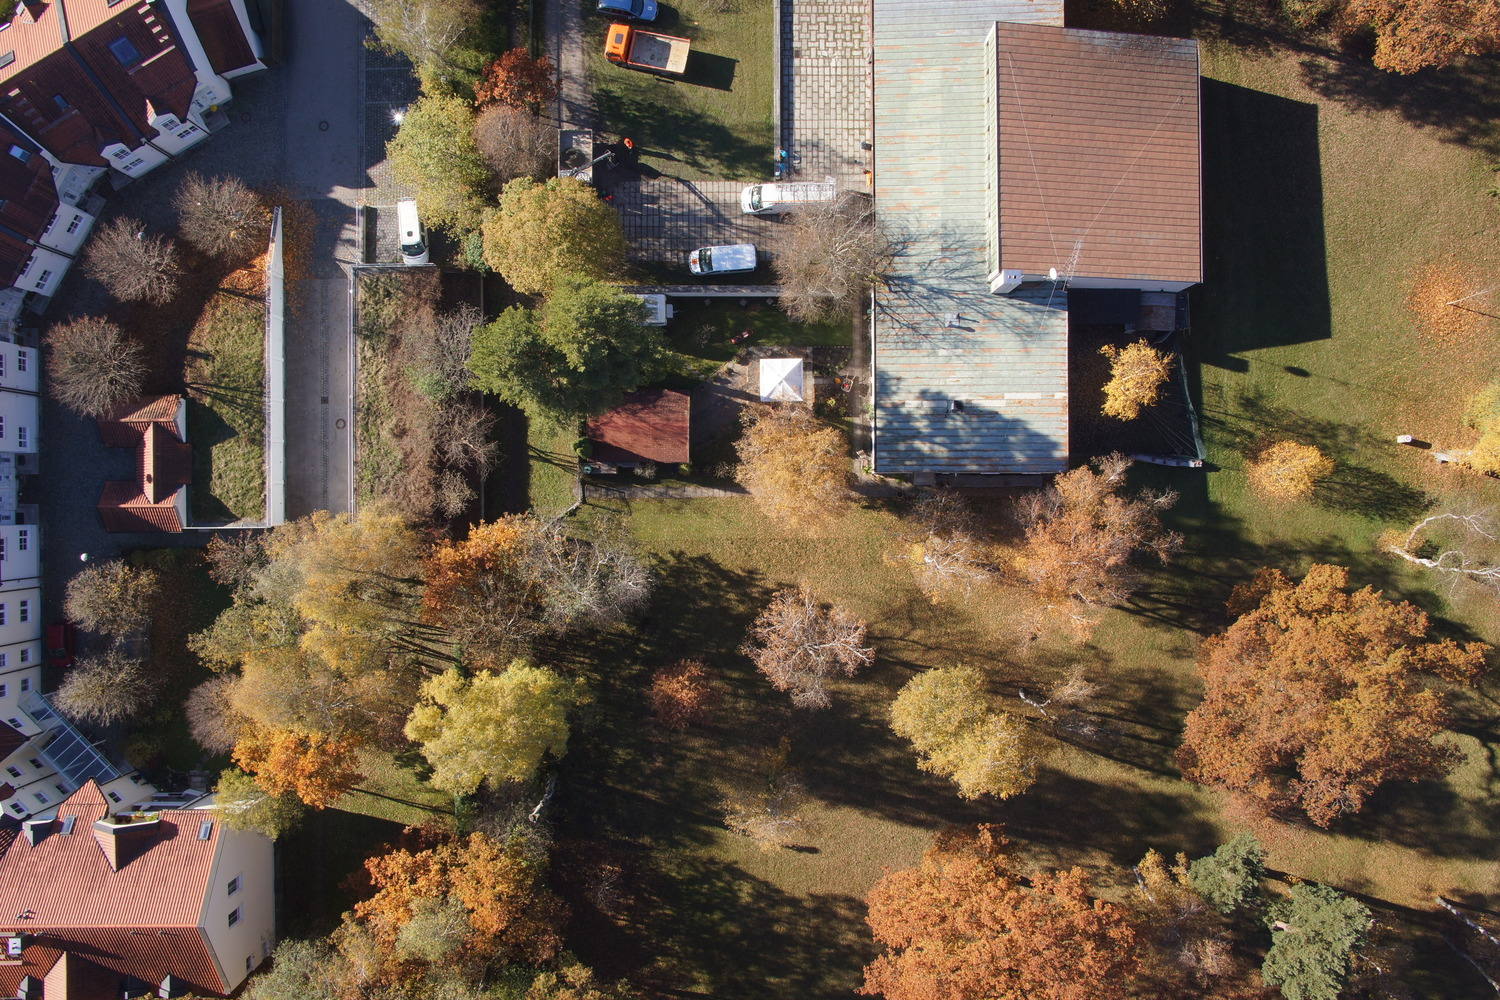
\includegraphics[width=1\linewidth]{fig/segmentation/DSC00793.JPG}
\end{subfigure}\vspace{1mm}
\begin{subfigure}{0.243\columnwidth}
  \centering
  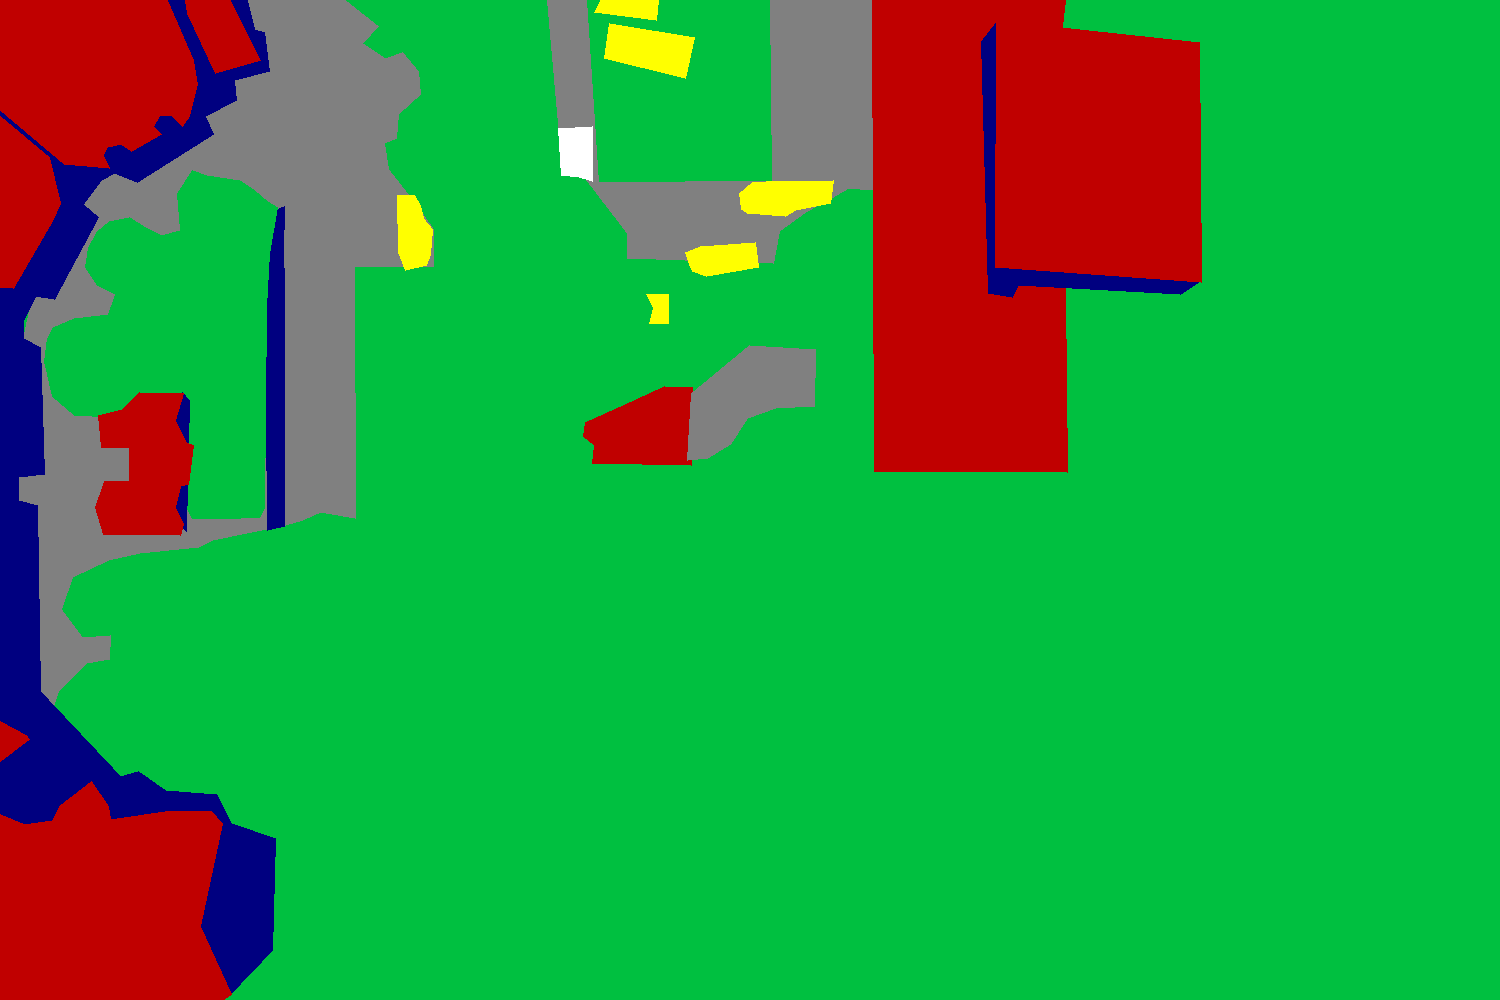
\includegraphics[width=1\linewidth]{fig/segmentation/DSC00793.png}
\end{subfigure}
\begin{subfigure}{0.243\columnwidth}
  \centering
  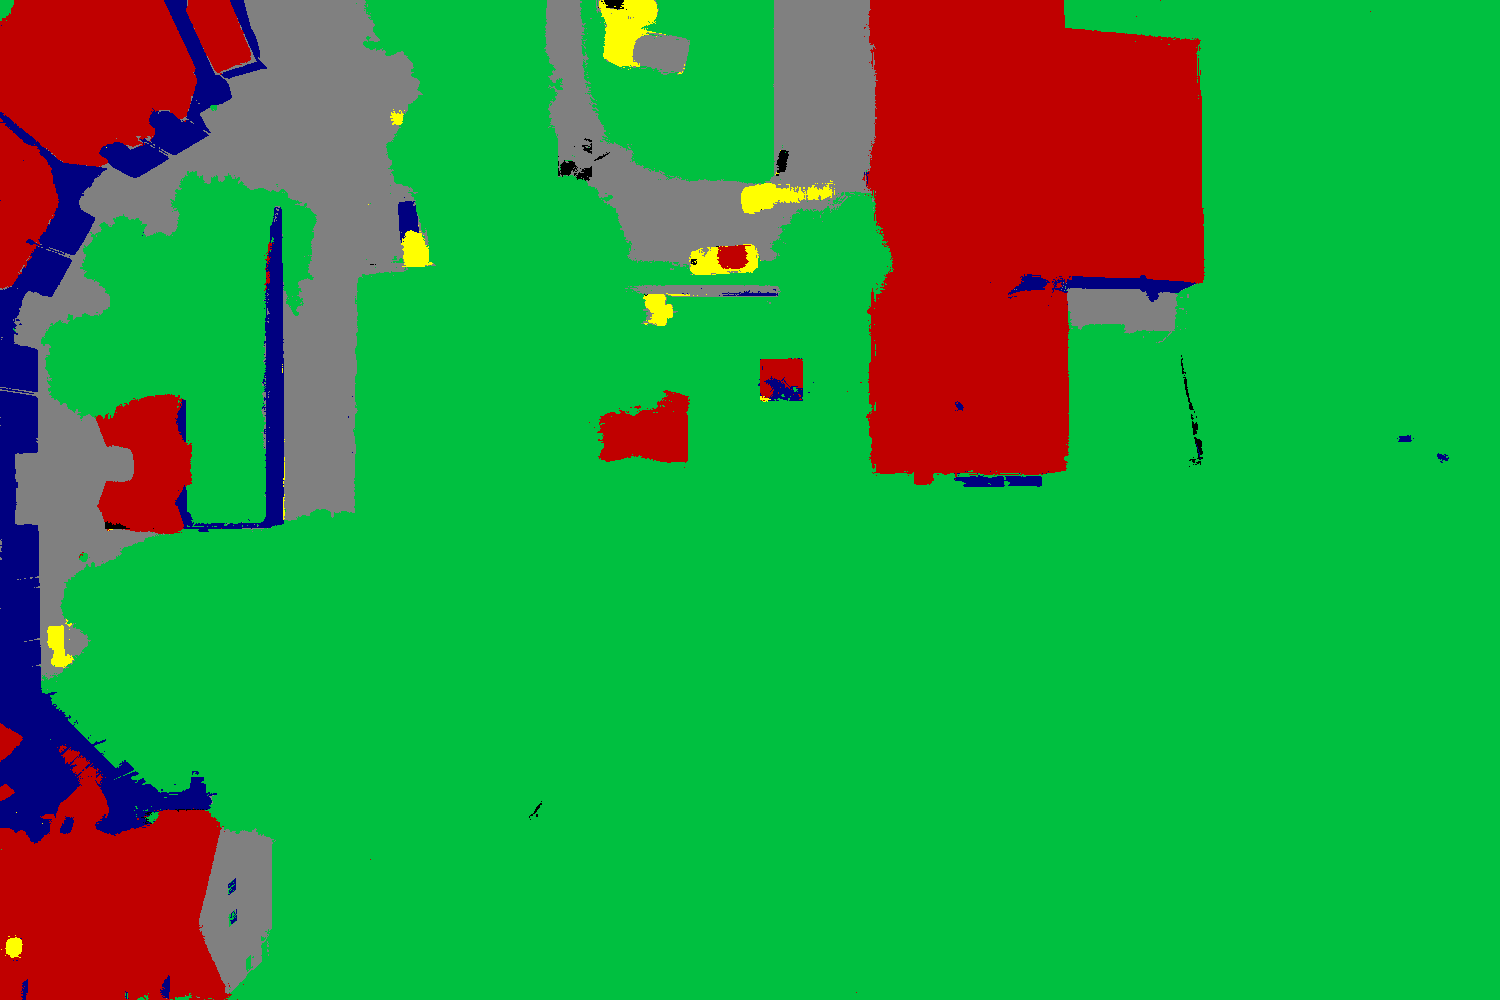
\includegraphics[width=1\linewidth]{fig/segmentation/DSC00793_6000_manualcrf.png}
\end{subfigure}
\begin{subfigure}{0.243\columnwidth}
  \centering
  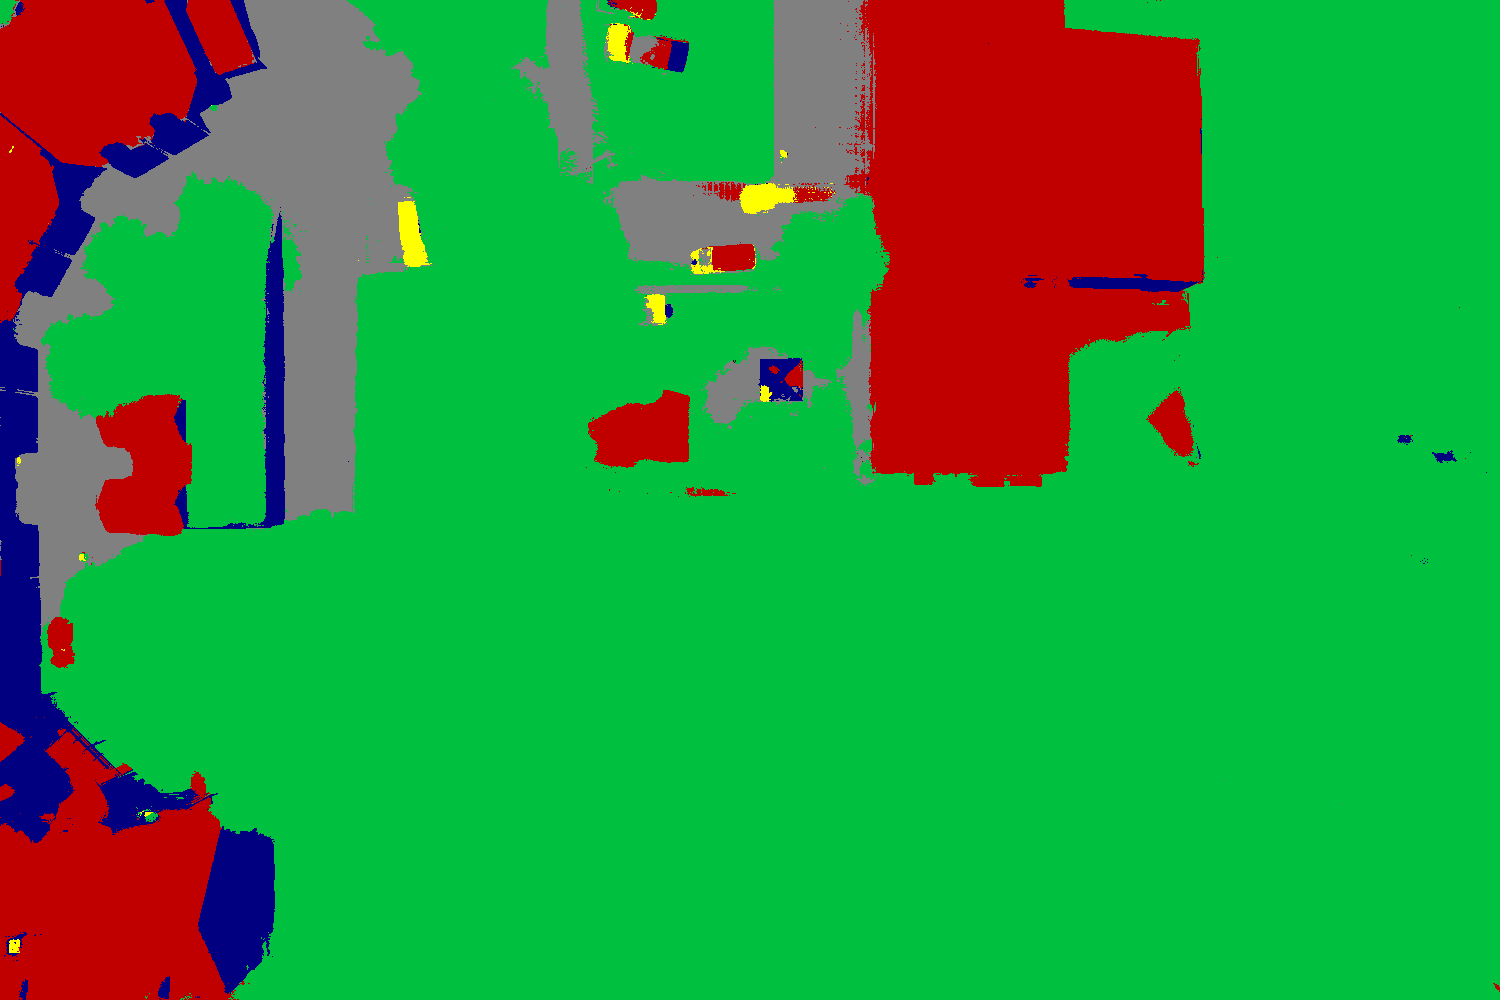
\includegraphics[width=1\linewidth]{fig/segmentation/DSC00793_6000_autocrf.png}
\end{subfigure}


\begin{subfigure}{0.243\columnwidth}
  \centering
  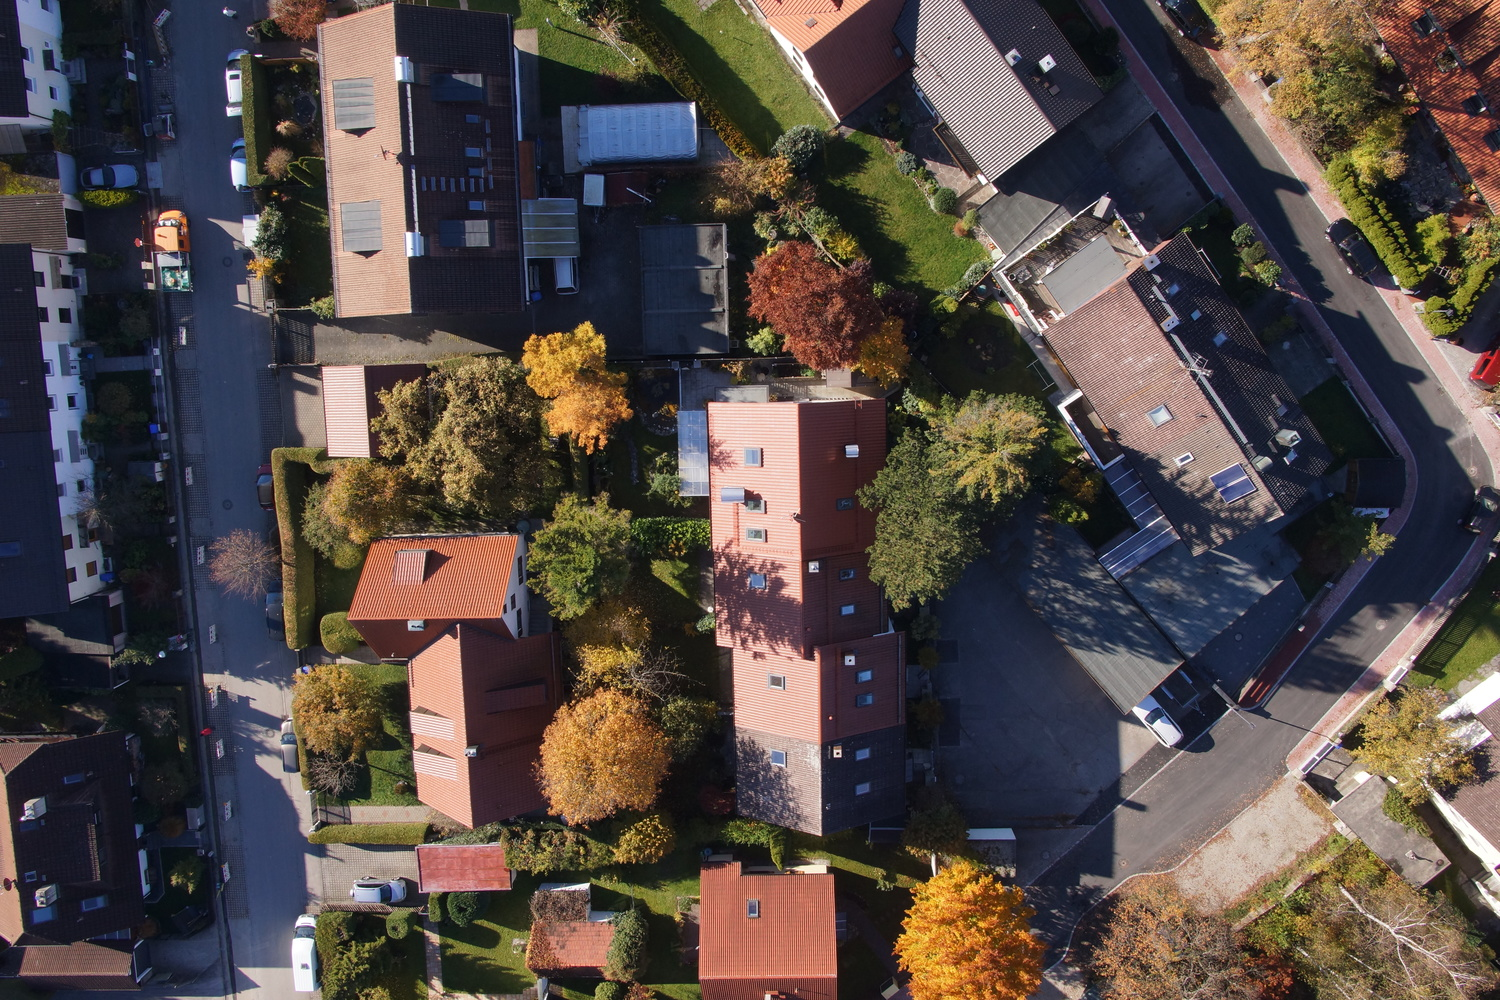
\includegraphics[width=1\linewidth]{fig/segmentation/DSC00837.JPG}
\end{subfigure}\vspace{1mm}
\begin{subfigure}{0.243\columnwidth}
  \centering
  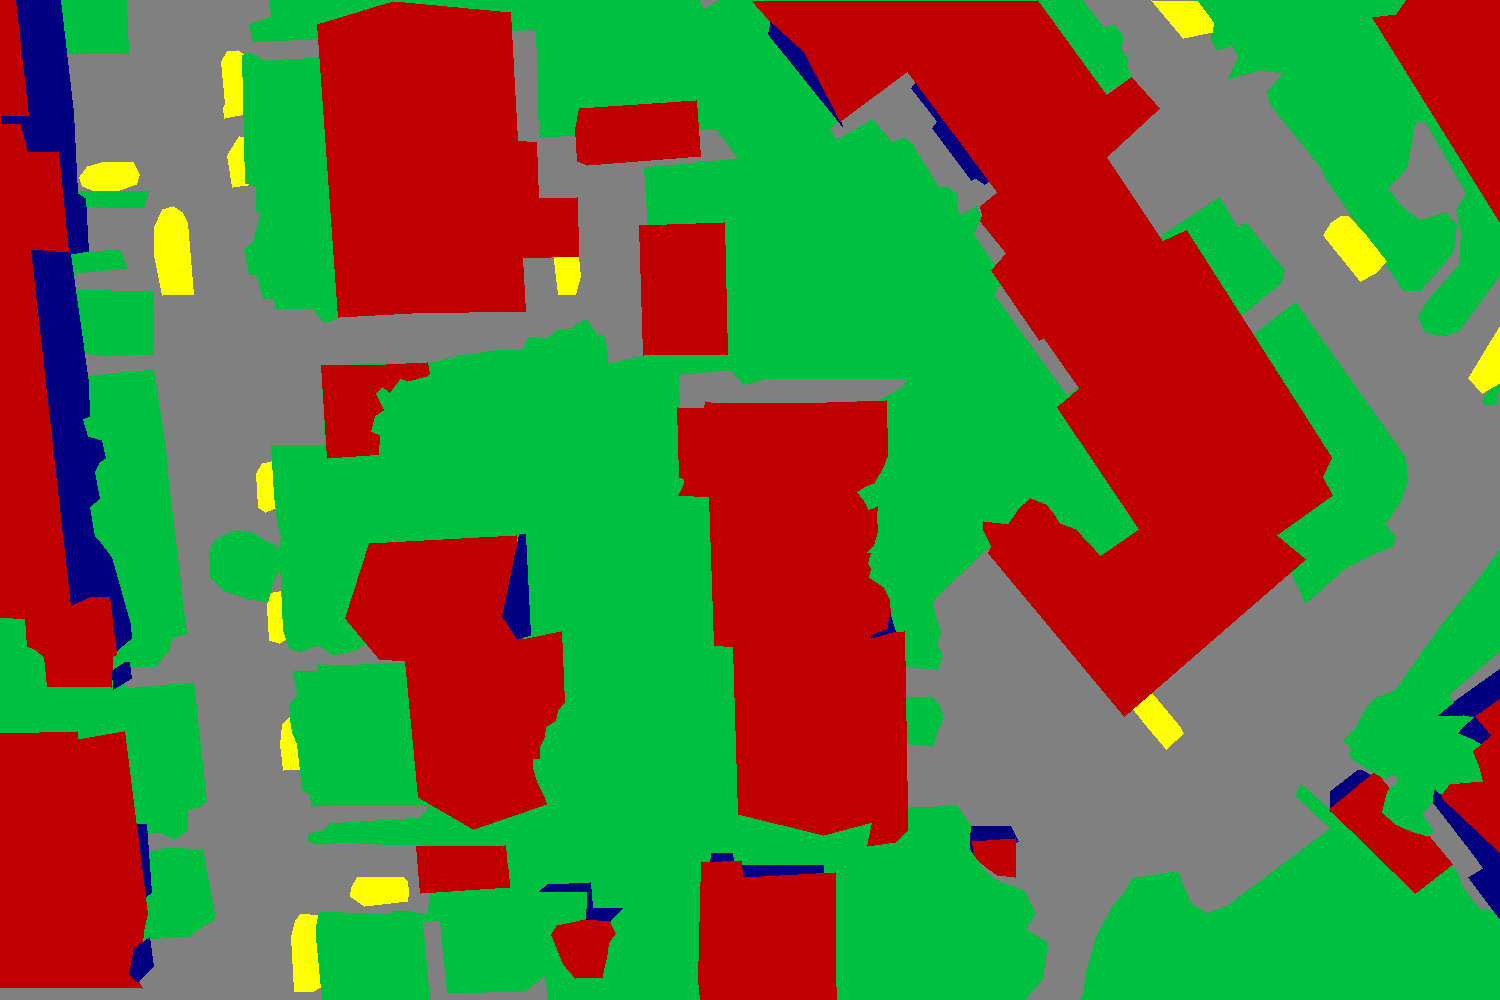
\includegraphics[width=1\linewidth]{fig/segmentation/DSC00837.png}
\end{subfigure}
\begin{subfigure}{0.243\columnwidth}
  \centering
  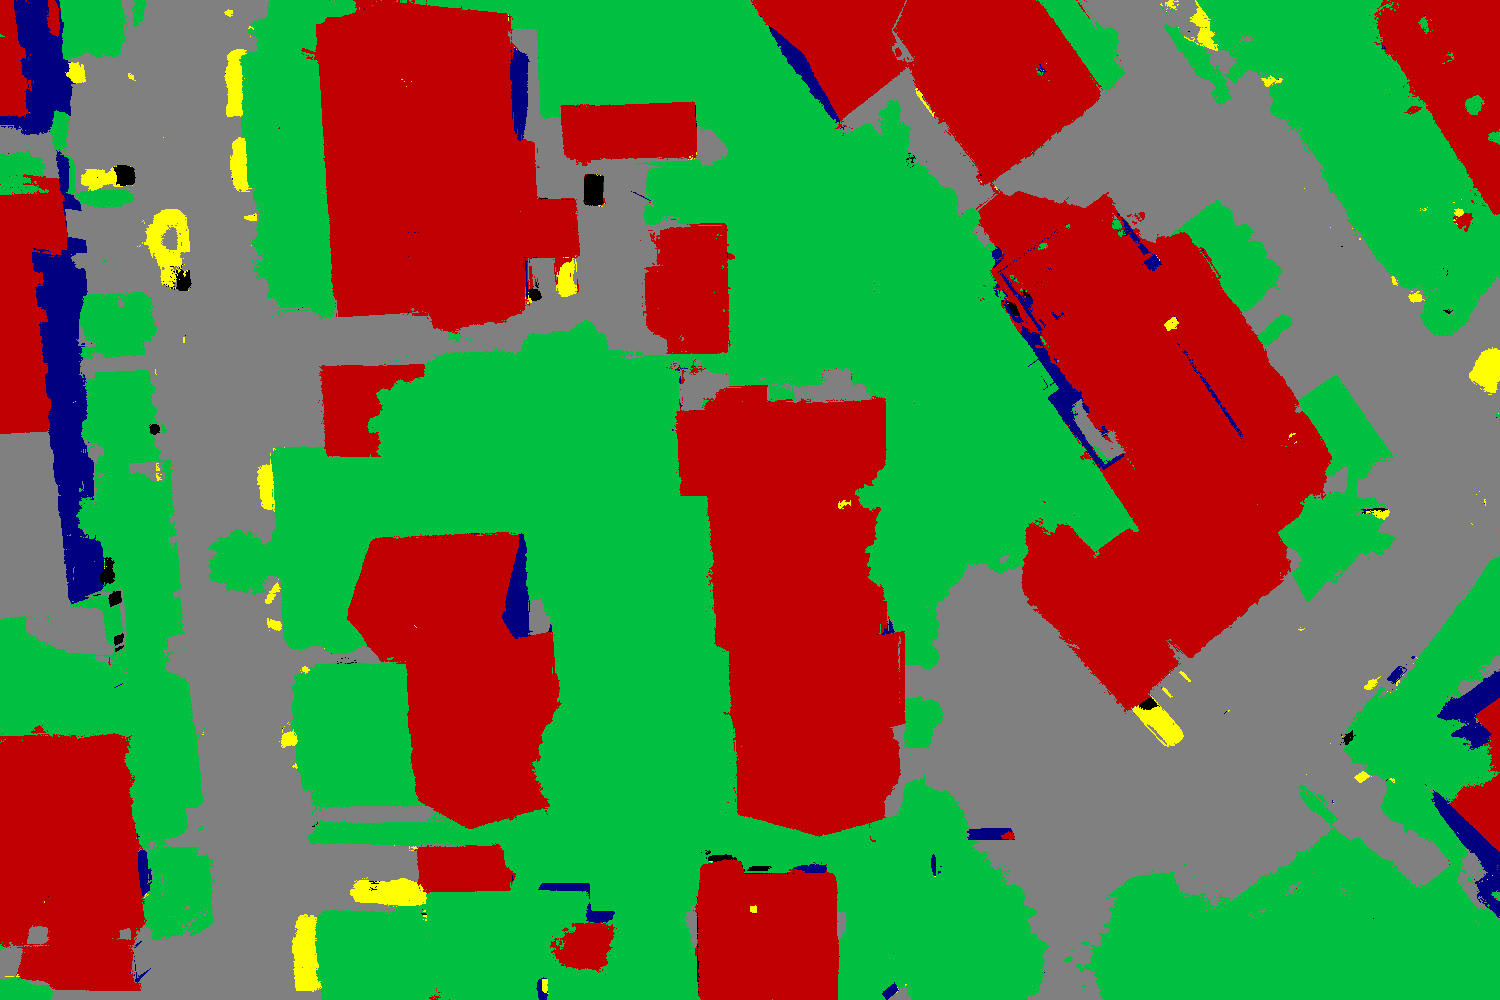
\includegraphics[width=1\linewidth]{fig/segmentation/DSC00837_6000_manualcrf.png}
\end{subfigure}
\begin{subfigure}{0.243\columnwidth}
  \centering
  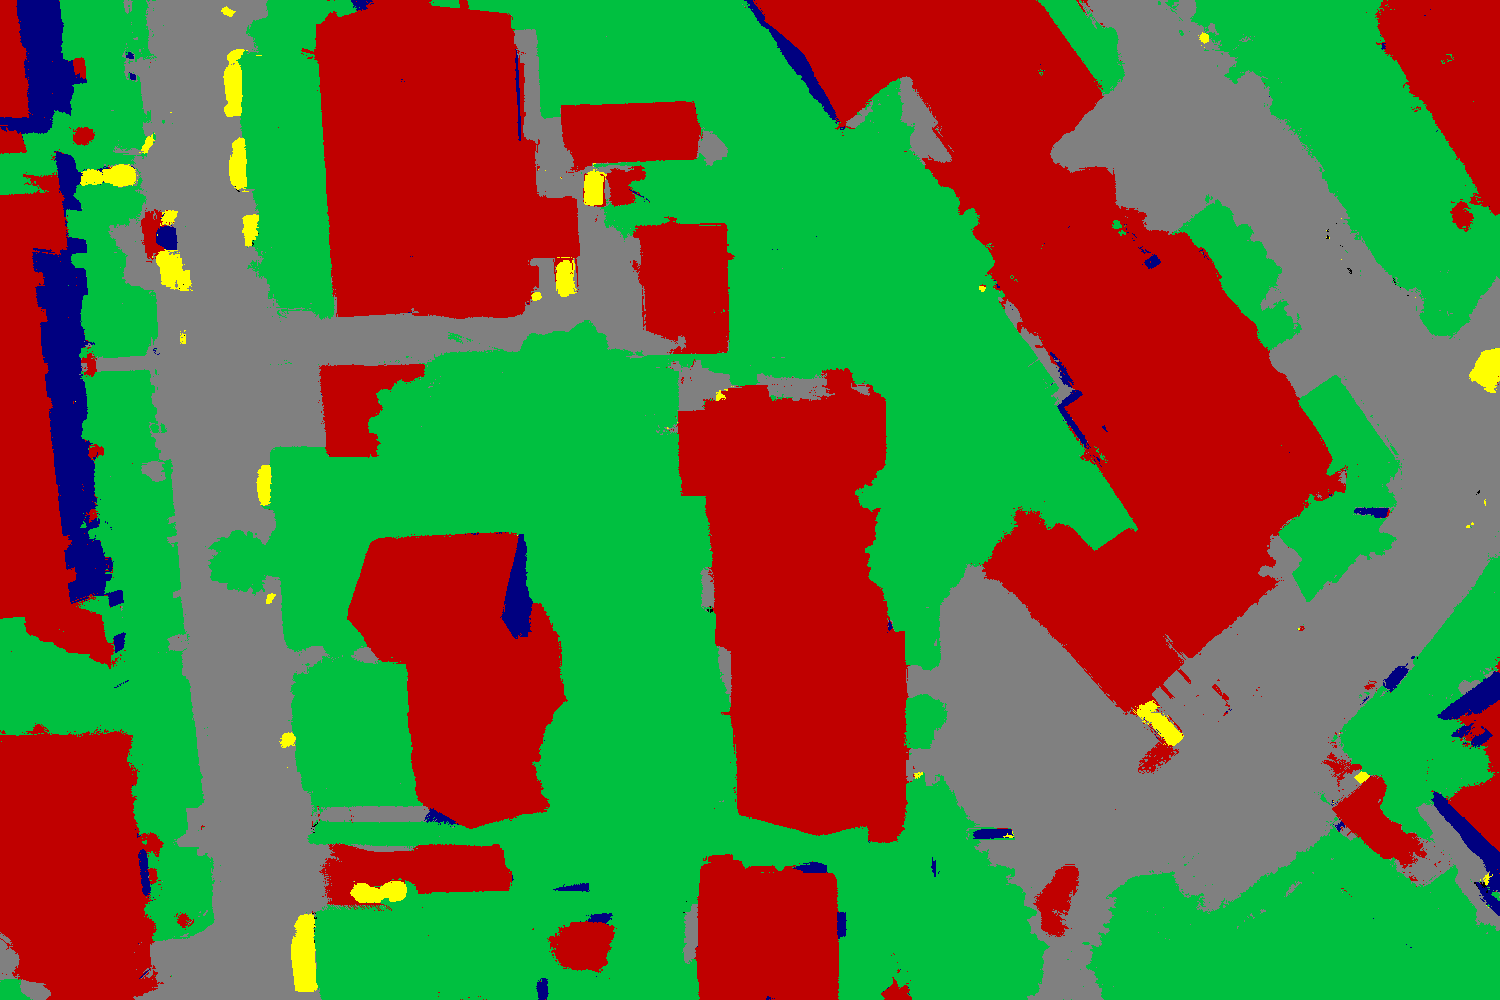
\includegraphics[width=1\linewidth]{fig/segmentation/DSC00837_6000_autocrf.png}
\end{subfigure}

\begin{subfigure}{0.243\columnwidth}
  \centering
  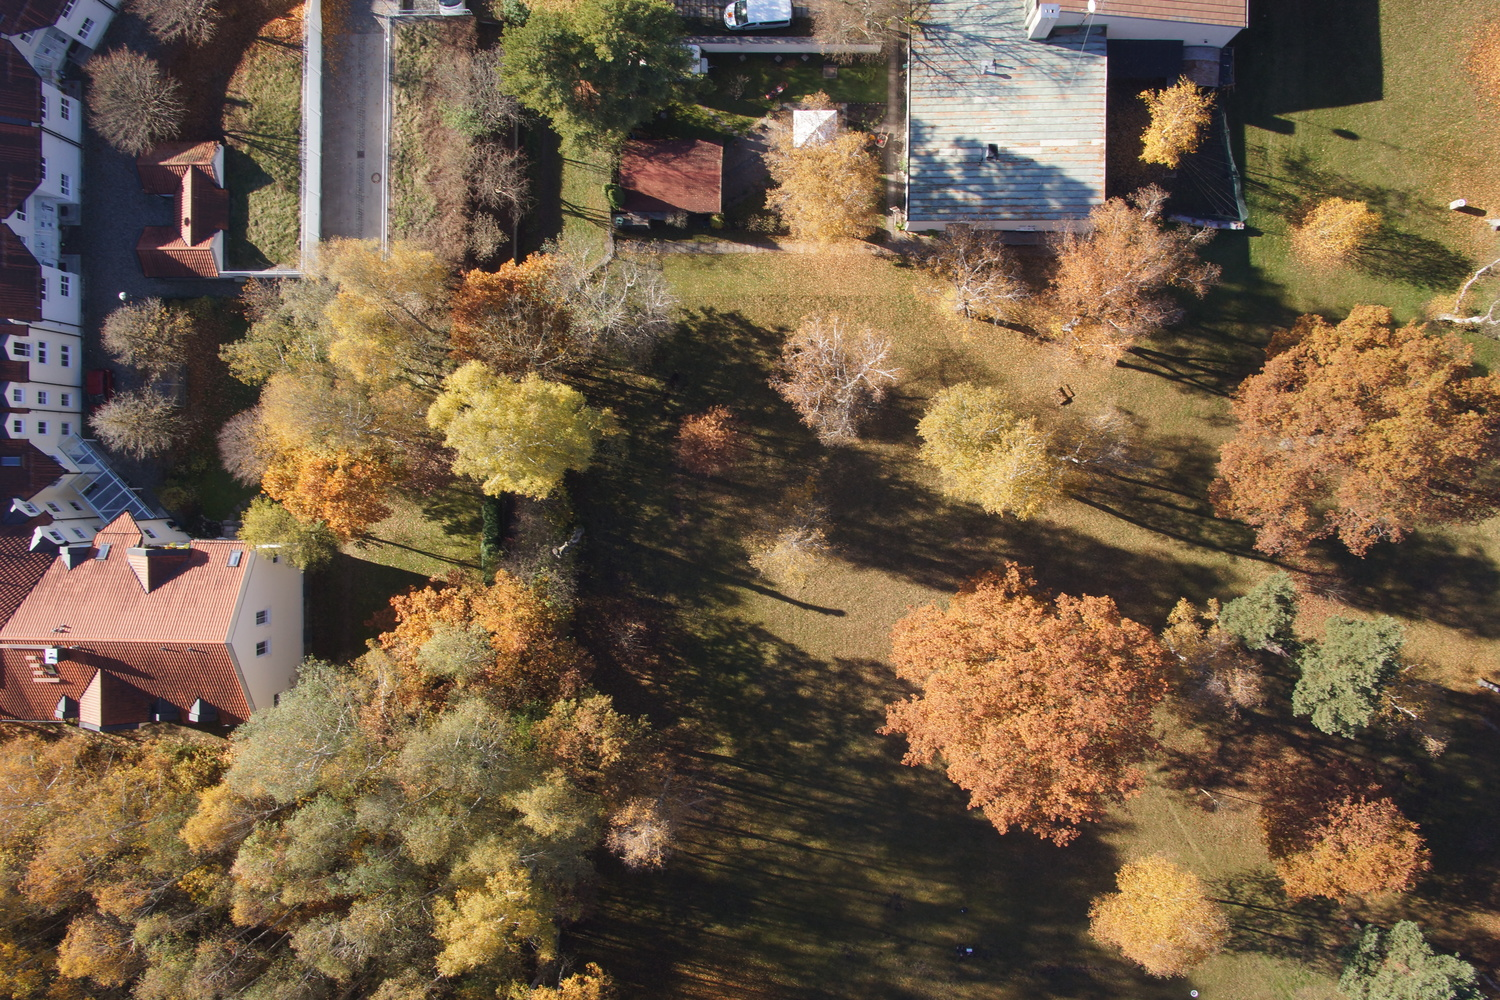
\includegraphics[width=1\linewidth]{fig/segmentation/DSC00792.JPG}
\end{subfigure}\vspace{1mm}
\begin{subfigure}{0.243\columnwidth}
  \centering
  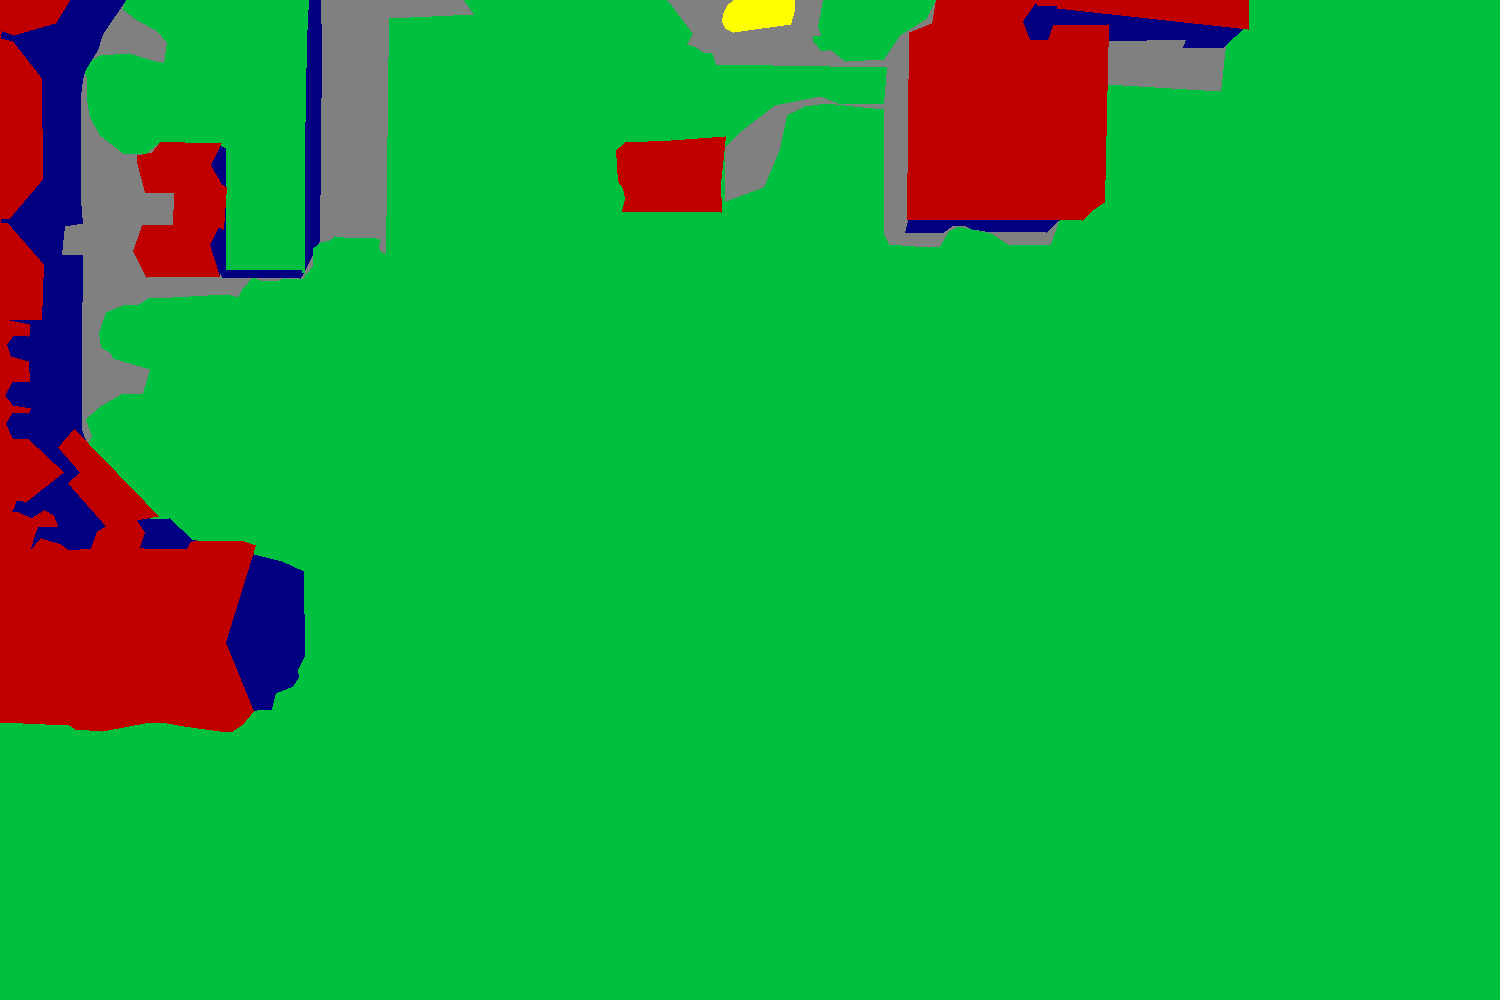
\includegraphics[width=1\linewidth]{fig/segmentation/DSC00792.png}
\end{subfigure}
\begin{subfigure}{0.243\columnwidth}
  \centering
  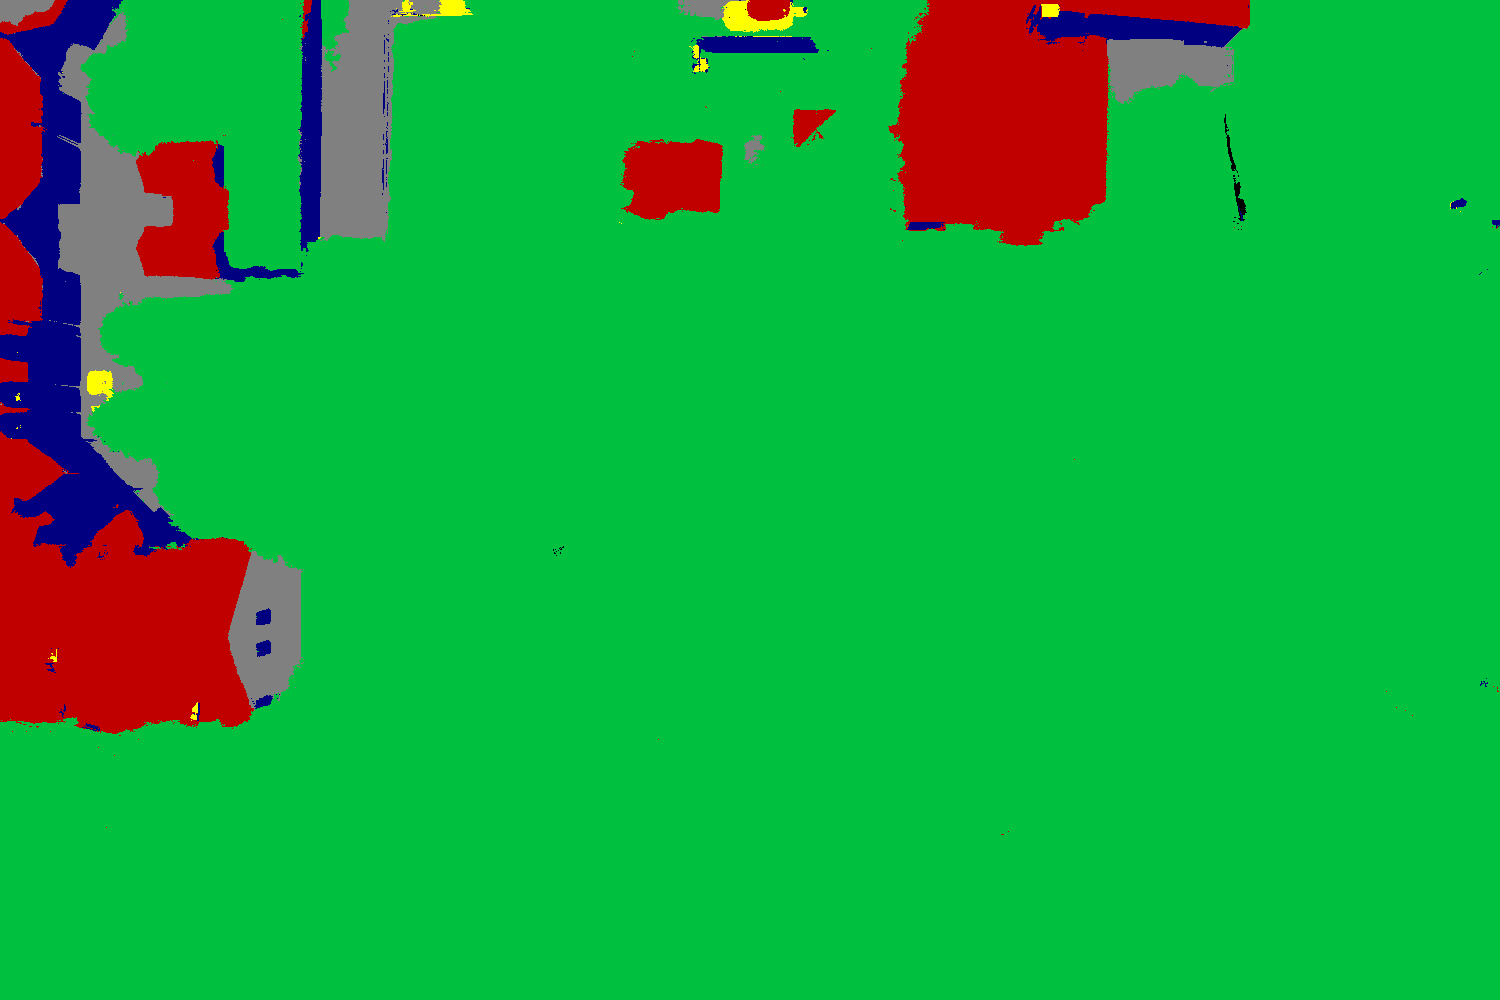
\includegraphics[width=1\linewidth]{fig/segmentation/DSC00792_6000_manualcrf.png}
\end{subfigure}
\begin{subfigure}{0.243\columnwidth}
  \centering
  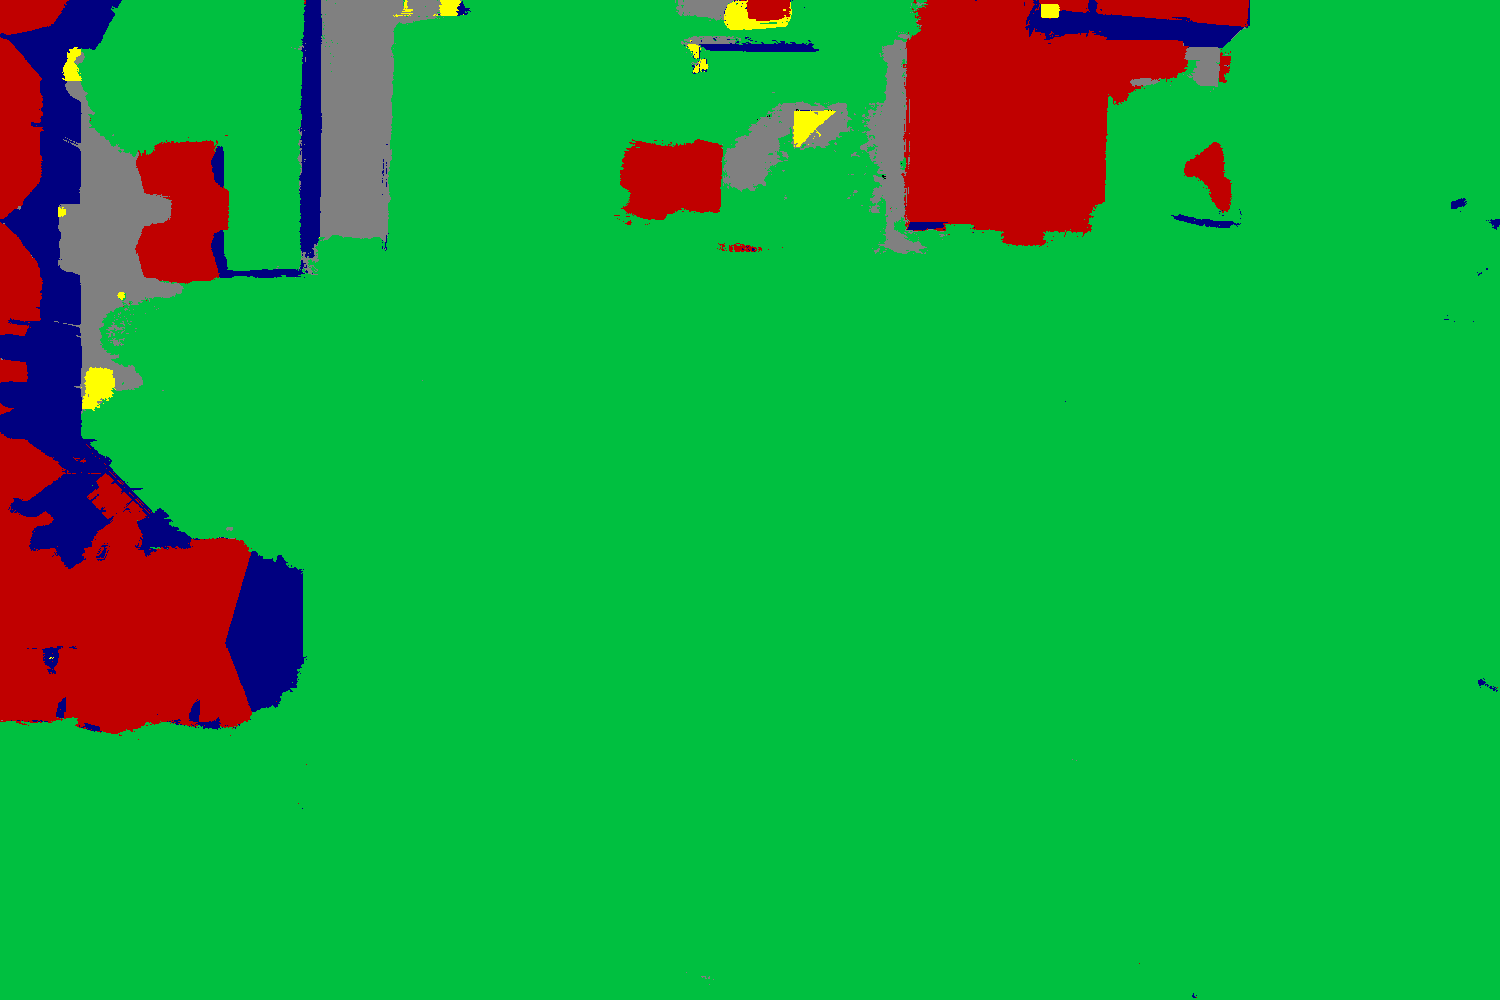
\includegraphics[width=1\linewidth]{fig/segmentation/DSC00792_6000_autocrf.png}
\end{subfigure}


\begin{subfigure}{0.243\columnwidth}
  \centering
  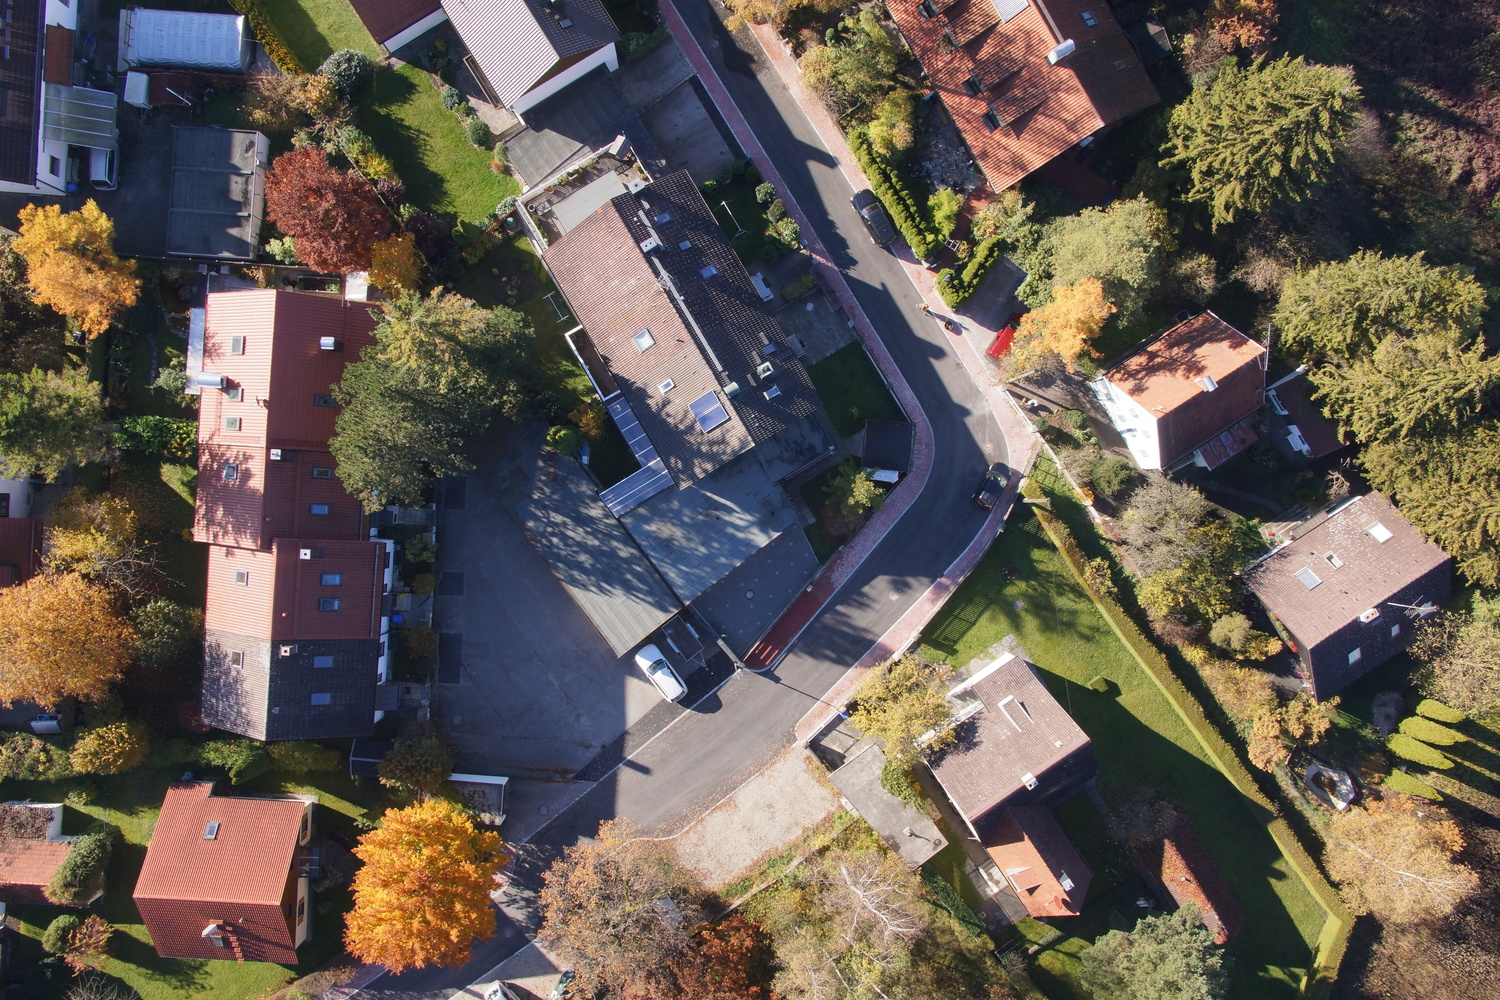
\includegraphics[width=1\linewidth]{fig/segmentation/DSC00849.JPG}
\end{subfigure}\vspace{1mm}
\begin{subfigure}{0.243\columnwidth}
  \centering
  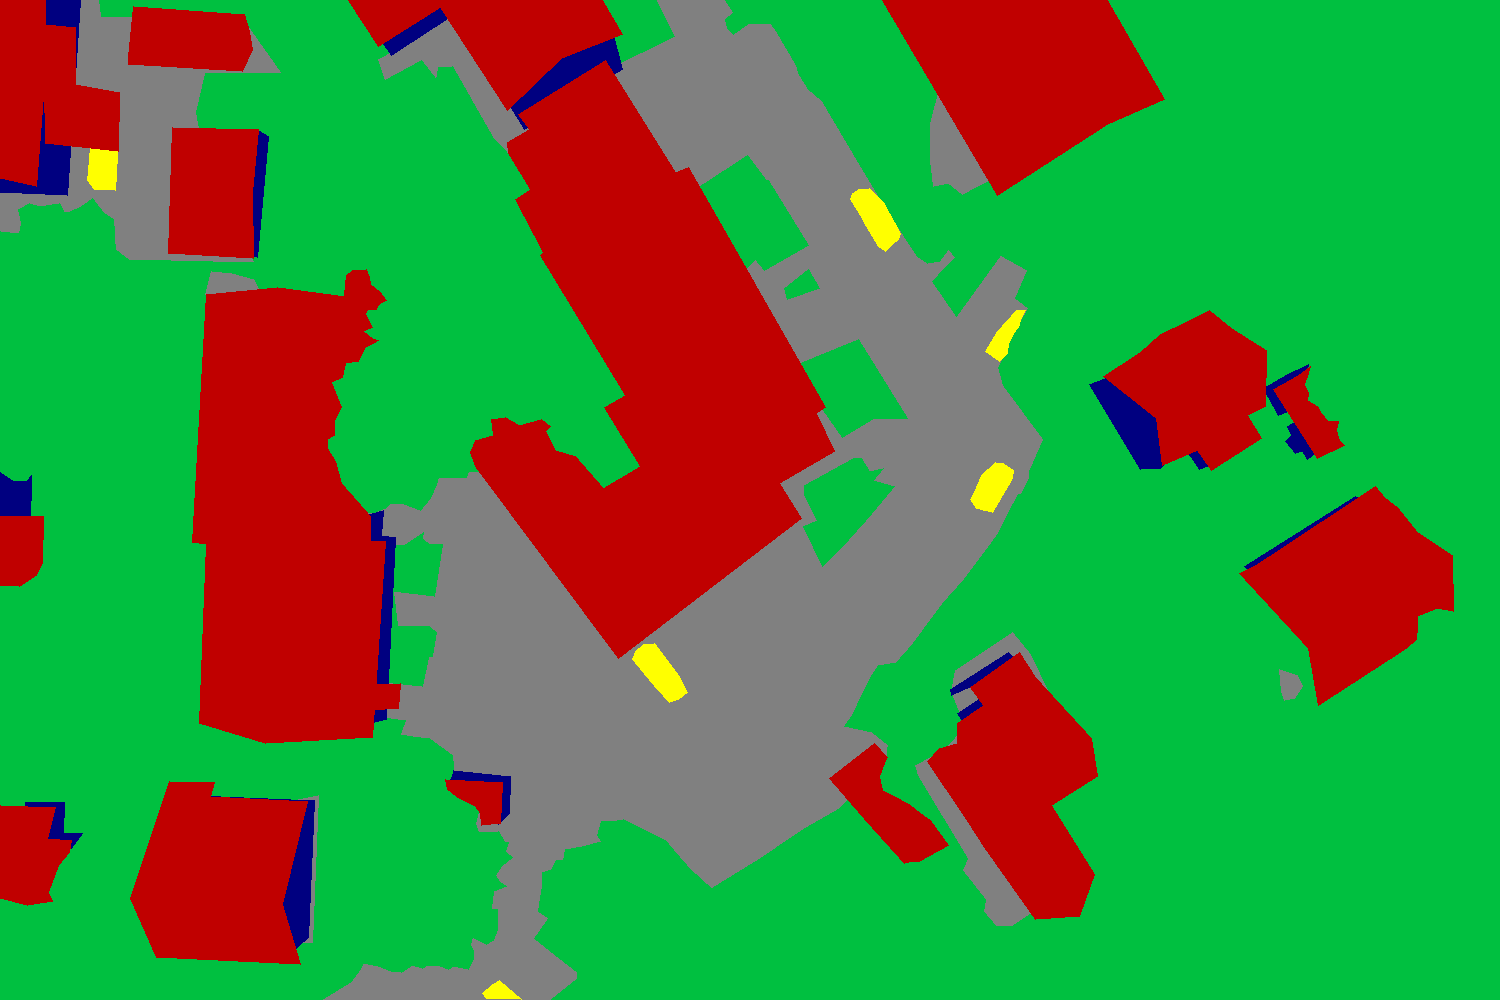
\includegraphics[width=1\linewidth]{fig/segmentation/DSC00849.png}
\end{subfigure}
\begin{subfigure}{0.243\columnwidth}
  \centering
  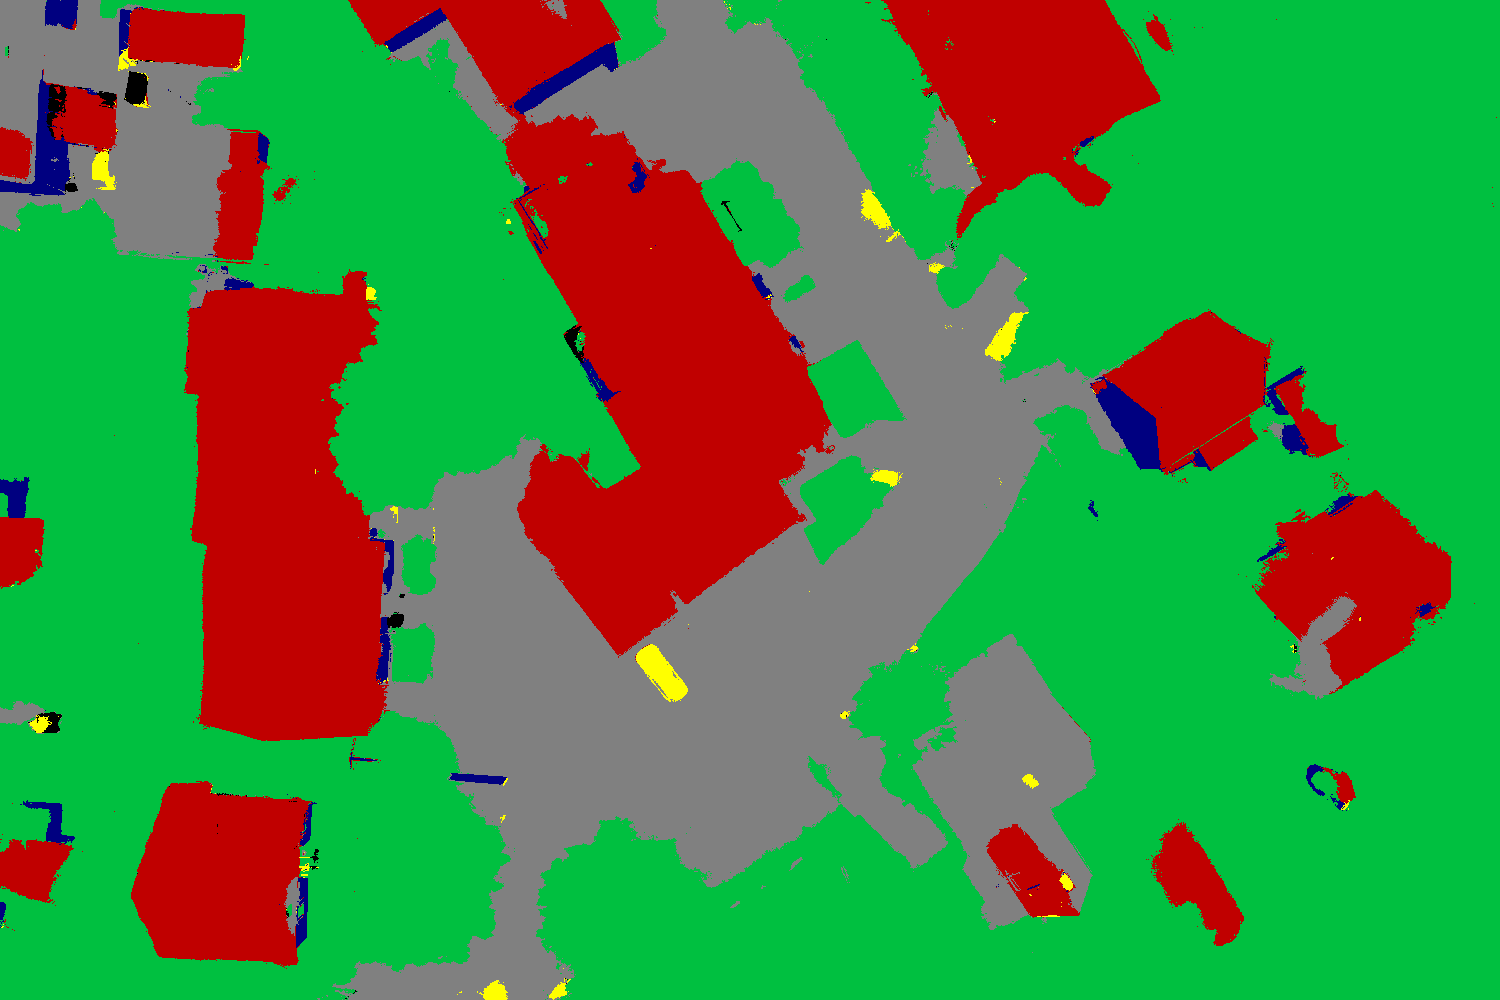
\includegraphics[width=1\linewidth]{fig/segmentation/DSC00849_6000_manualcrf.png}
\end{subfigure}
\begin{subfigure}{0.243\columnwidth}
  \centering
  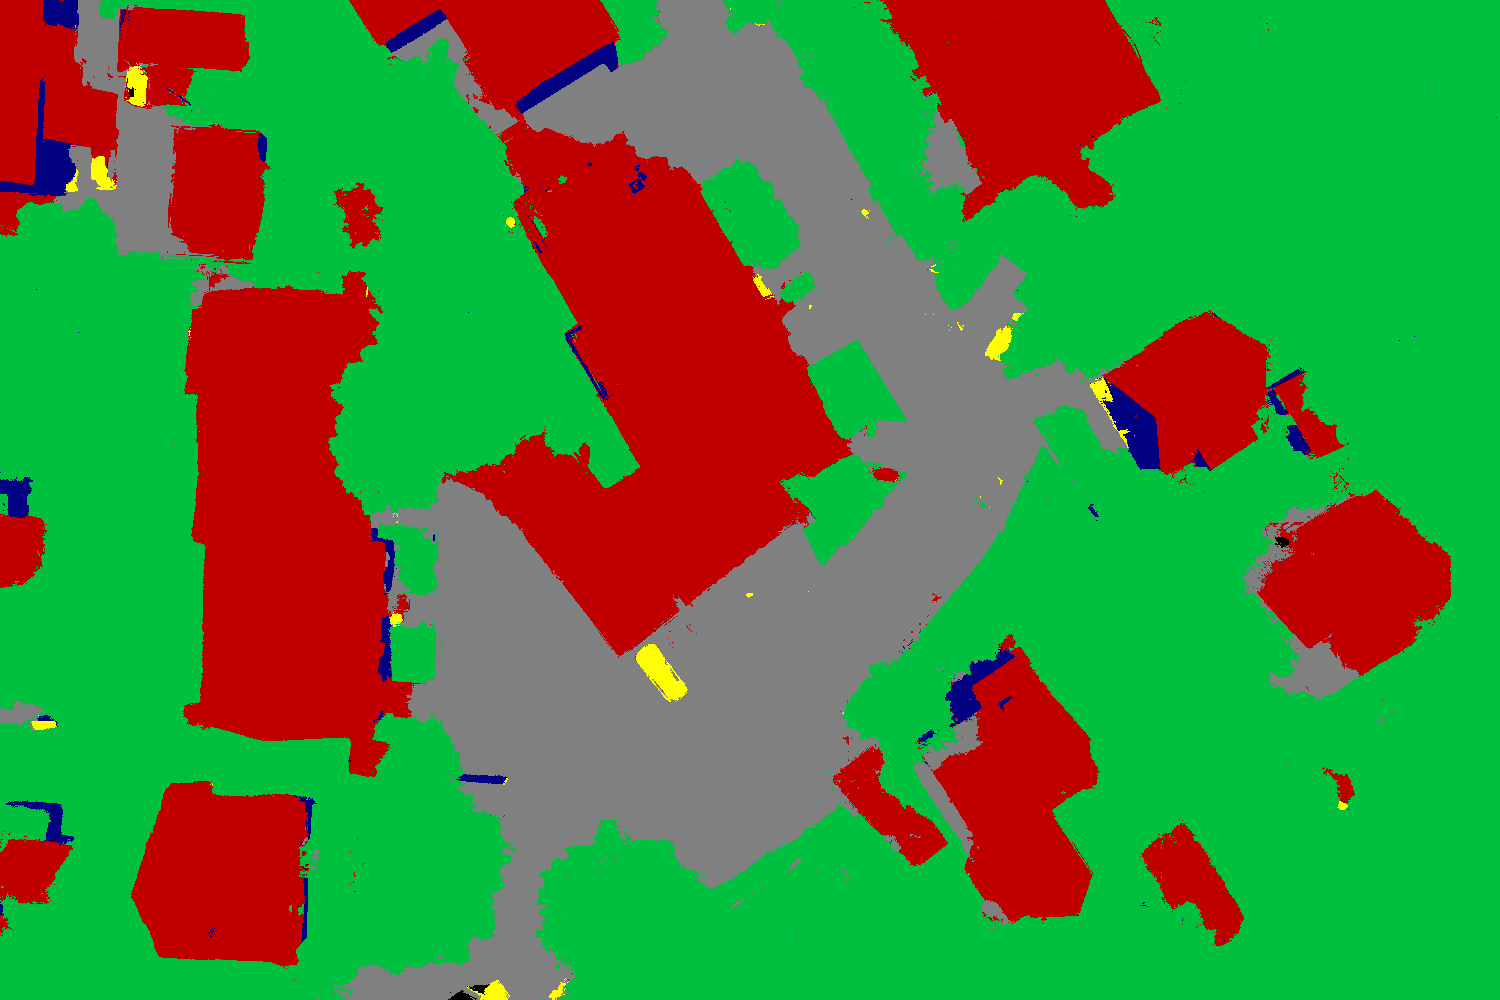
\includegraphics[width=1\linewidth]{fig/segmentation/DSC00849_6000_autocrf.png}
\end{subfigure}


\begin{subfigure}{0.243\columnwidth}
  \centering
  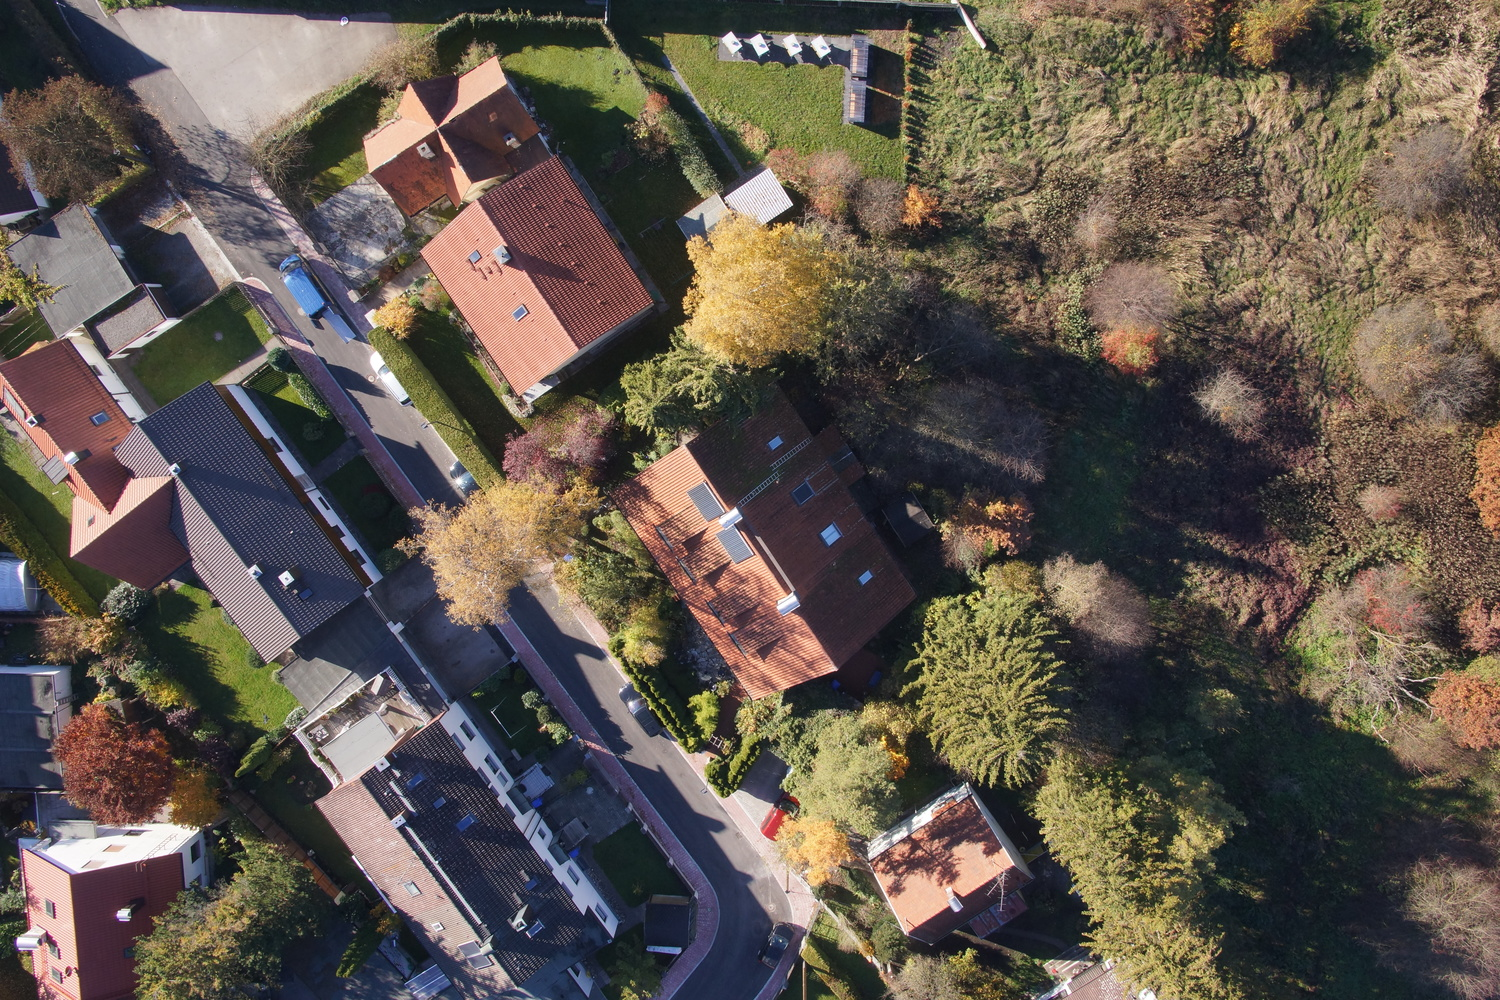
\includegraphics[width=1\linewidth]{fig/segmentation/DSC00855.JPG}
  \caption{}
\end{subfigure}
\begin{subfigure}{0.243\columnwidth}
  \centering
  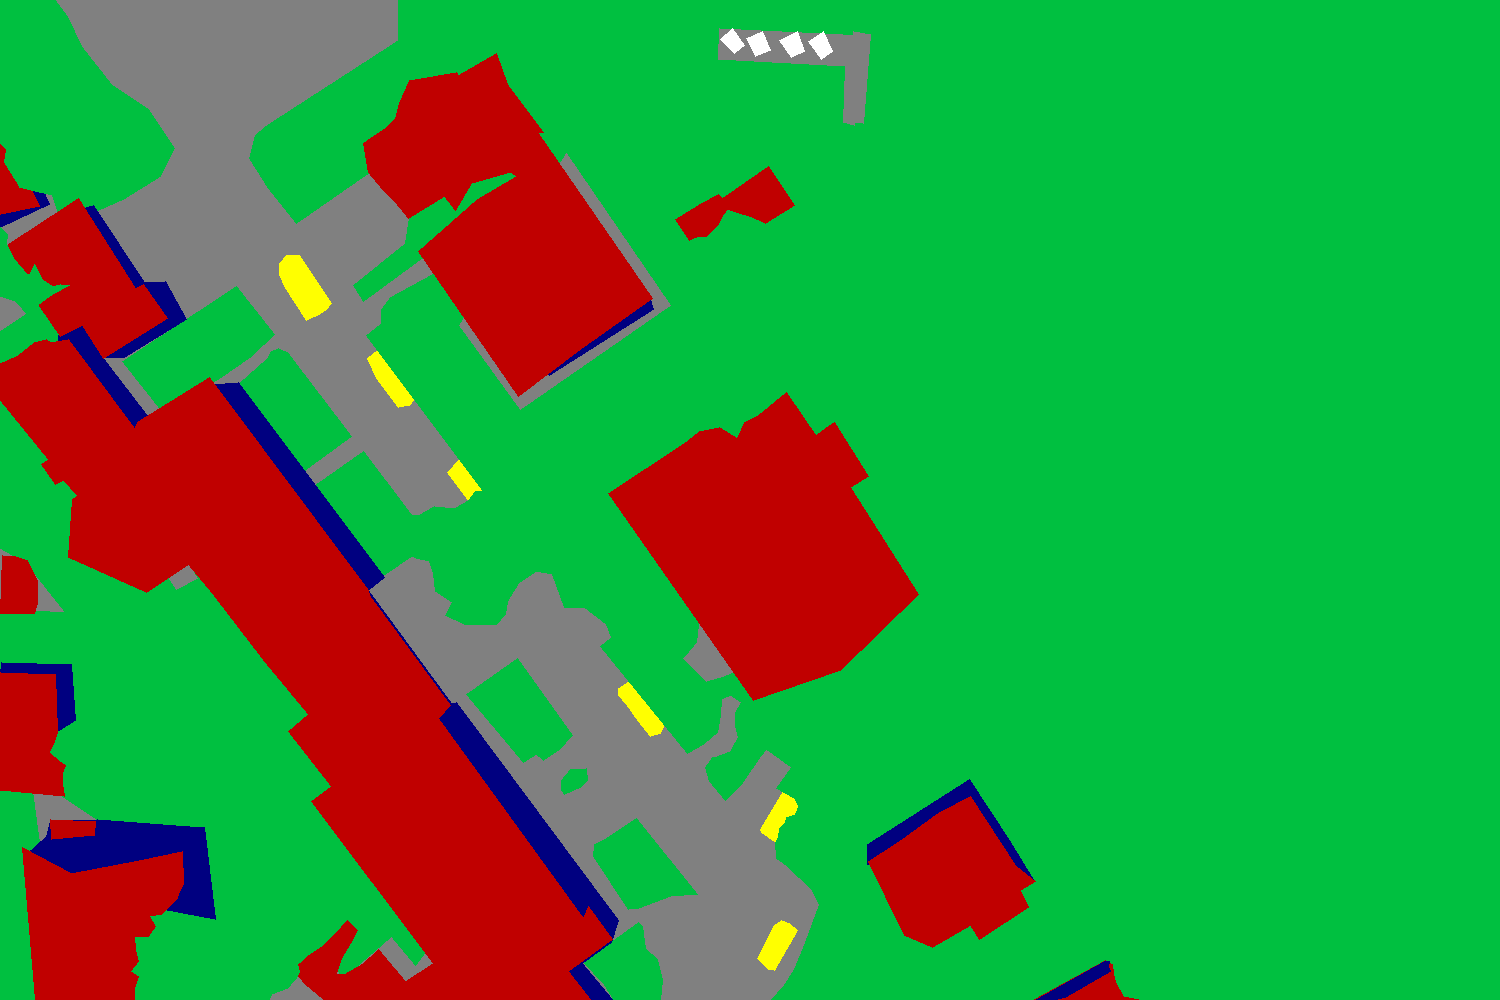
\includegraphics[width=1\linewidth]{fig/segmentation/DSC00855.png}
  \caption{}
\end{subfigure}
\begin{subfigure}{0.243\columnwidth}
  \centering
  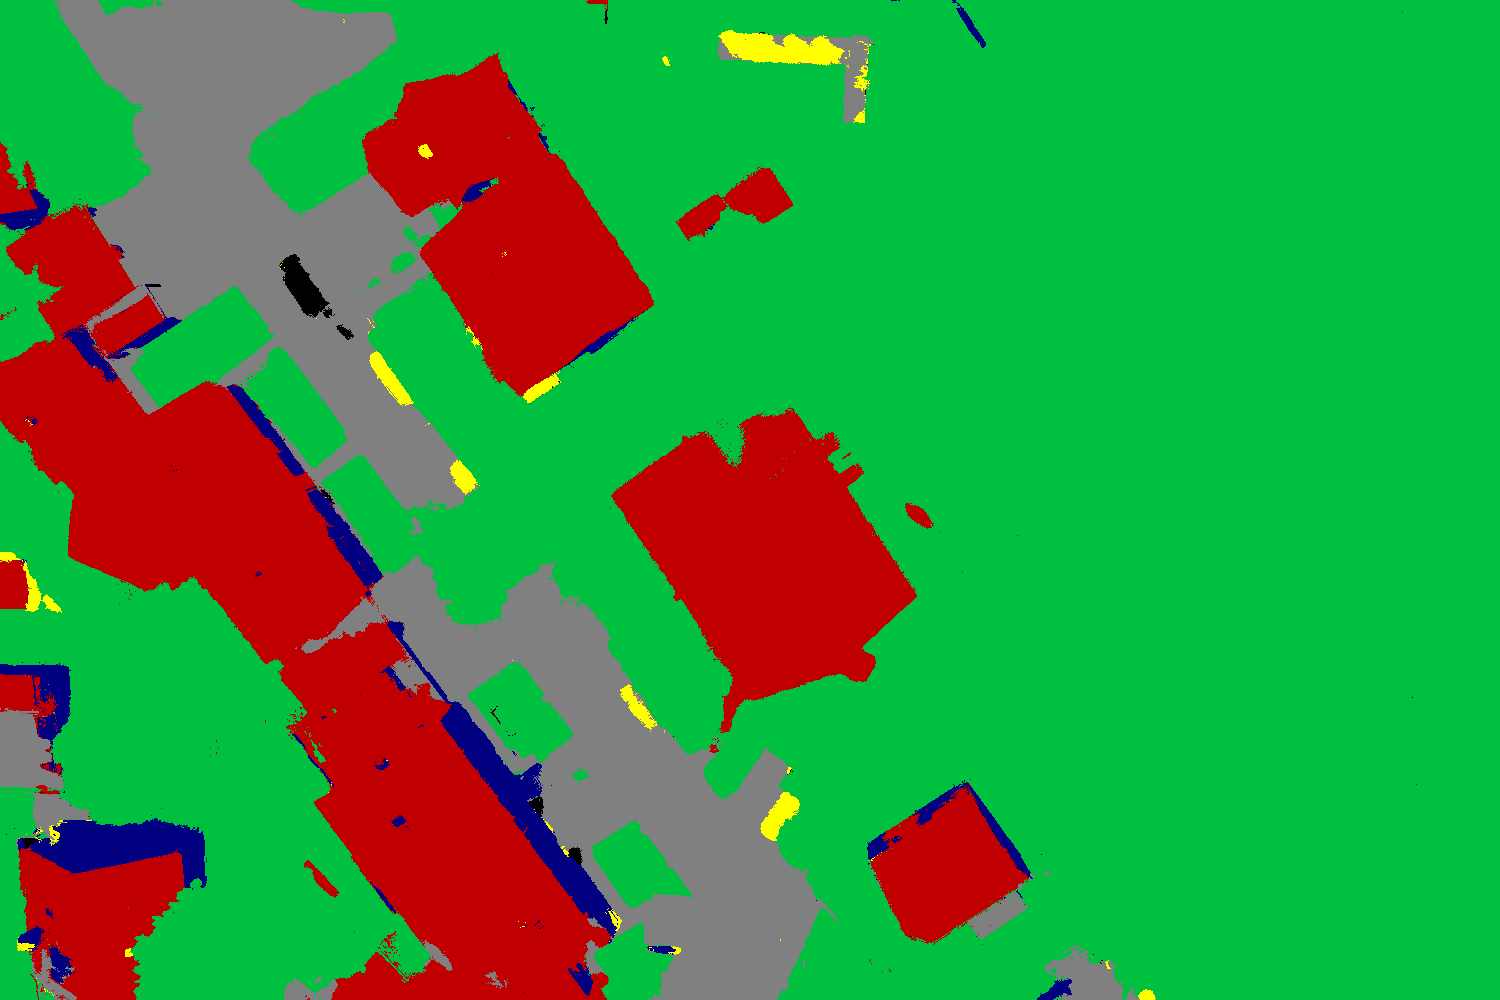
\includegraphics[width=1\linewidth]{fig/segmentation/DSC00855_6000_manualcrf.png}
  \caption{}
\end{subfigure}
\begin{subfigure}{0.243\columnwidth}
  \centering
  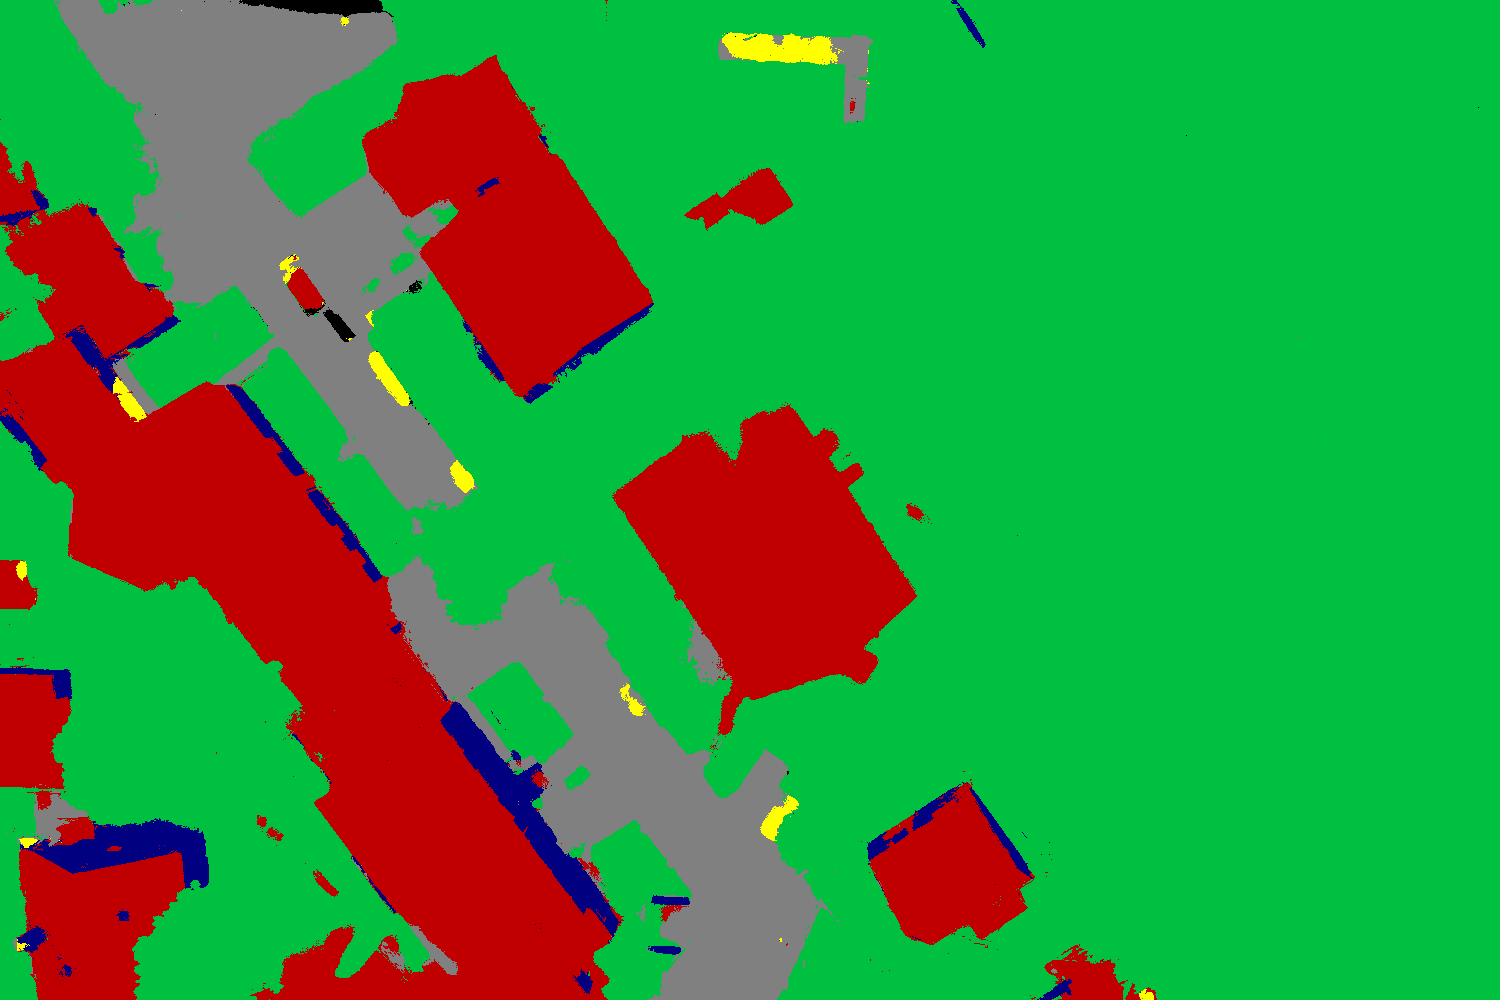
\includegraphics[width=1\linewidth]{fig/segmentation/DSC00855_6000_autocrf.png}
  \caption{}
\end{subfigure}

\caption{Comparison of predictions on \textbf{Area 1}. (a) original UAV images, (b) corresponding ground-truth, (c) predictions using manually annotated training data, (d) predictions using automatically generated training data.}
\label{fig:seg_ei}
\end{figure}



\begin{table}[htb]
\centering
\caption{Comparison of segmentation accuracy (IoU) using automatic training data and manual training data.}
\label{seg}
    \begin{tabular}{cccccc}
    \toprule
    \textbf{} & \textbf{Roof} & \textbf{Building} & \textbf{Veg} & \textbf{Car} & \textbf{Ground} \\
    %Define if appropriate
          
    \midrule

Manual    &  84.43 &     56.47 & 94.17  & 39.74 & 74.47\\
Inferred &   87.48 &   61.93   &    93.79  & 36.21& 78.09\\
% M    &  89.42 &     50.93 & 95.99  & 41.40 & 76.23\\\hline
\bottomrule
\end{tabular}
\end{table}

\subsection{Generating Image Annotation on a Scale}
The superiority of the proposed method lies also in its ability to generate image annotations on a scale. Due to the high expense of time and labor, the quantity of manually labeled ground-truth data is limited and sometimes not enough to achieve reasonable segmentation performance. By contrast, our method can generate image annotations on a large scale exempt from manual work, ensuring sufficient amount of training data. To verify the impact of training data quantity, we applied the network trained with the manual annotations (23 image frames) for image segmentation in \textbf{Area 2}. The predictions, as shown in Figure \ref{fig:area2}-(b), demonstrate deficient accuracy. In contrast, we generated annotations for 72 image frames of \textbf{Area 1} by automatic inference, and then used them to train a CNN. Afterwards, we tested the trained network for image segmentation in \textbf{Area 2}. The prediction results, as depicted in Figure \ref{fig:area2}-(c), demonstrate apparently better semantic accuracy. 

\begin{figure}[htb]
\begin{subfigure}{0.32\columnwidth}
  \centering
  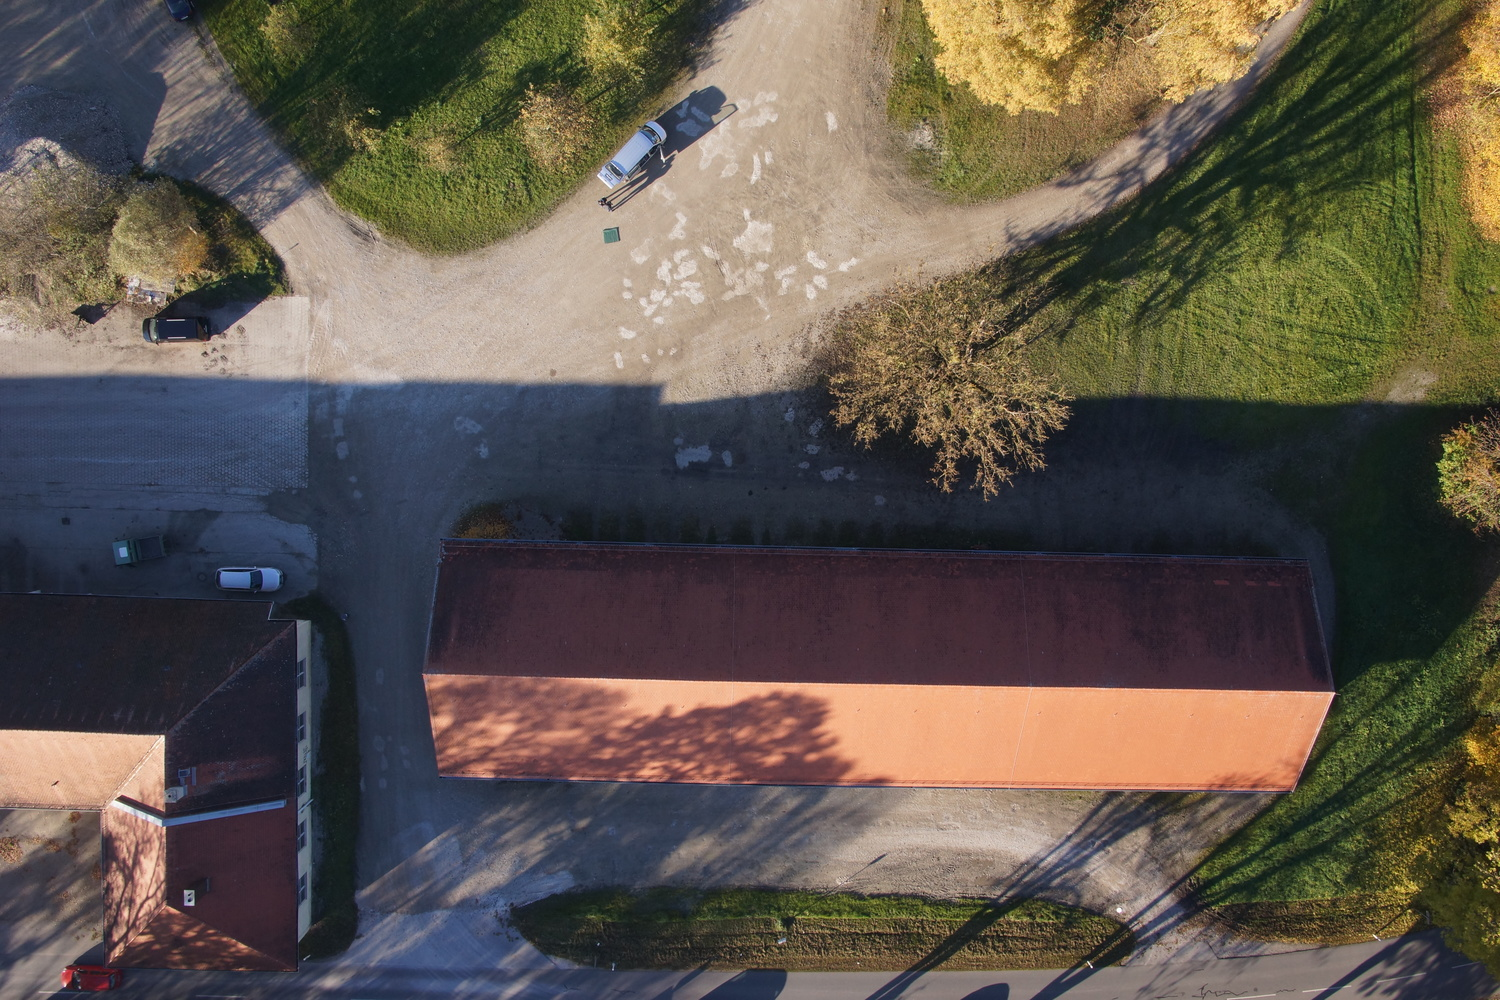
\includegraphics[width=1\linewidth]{fig/segmentation/DSC00958.JPG}

\end{subfigure}
\begin{subfigure}{0.32\columnwidth}
  \centering
  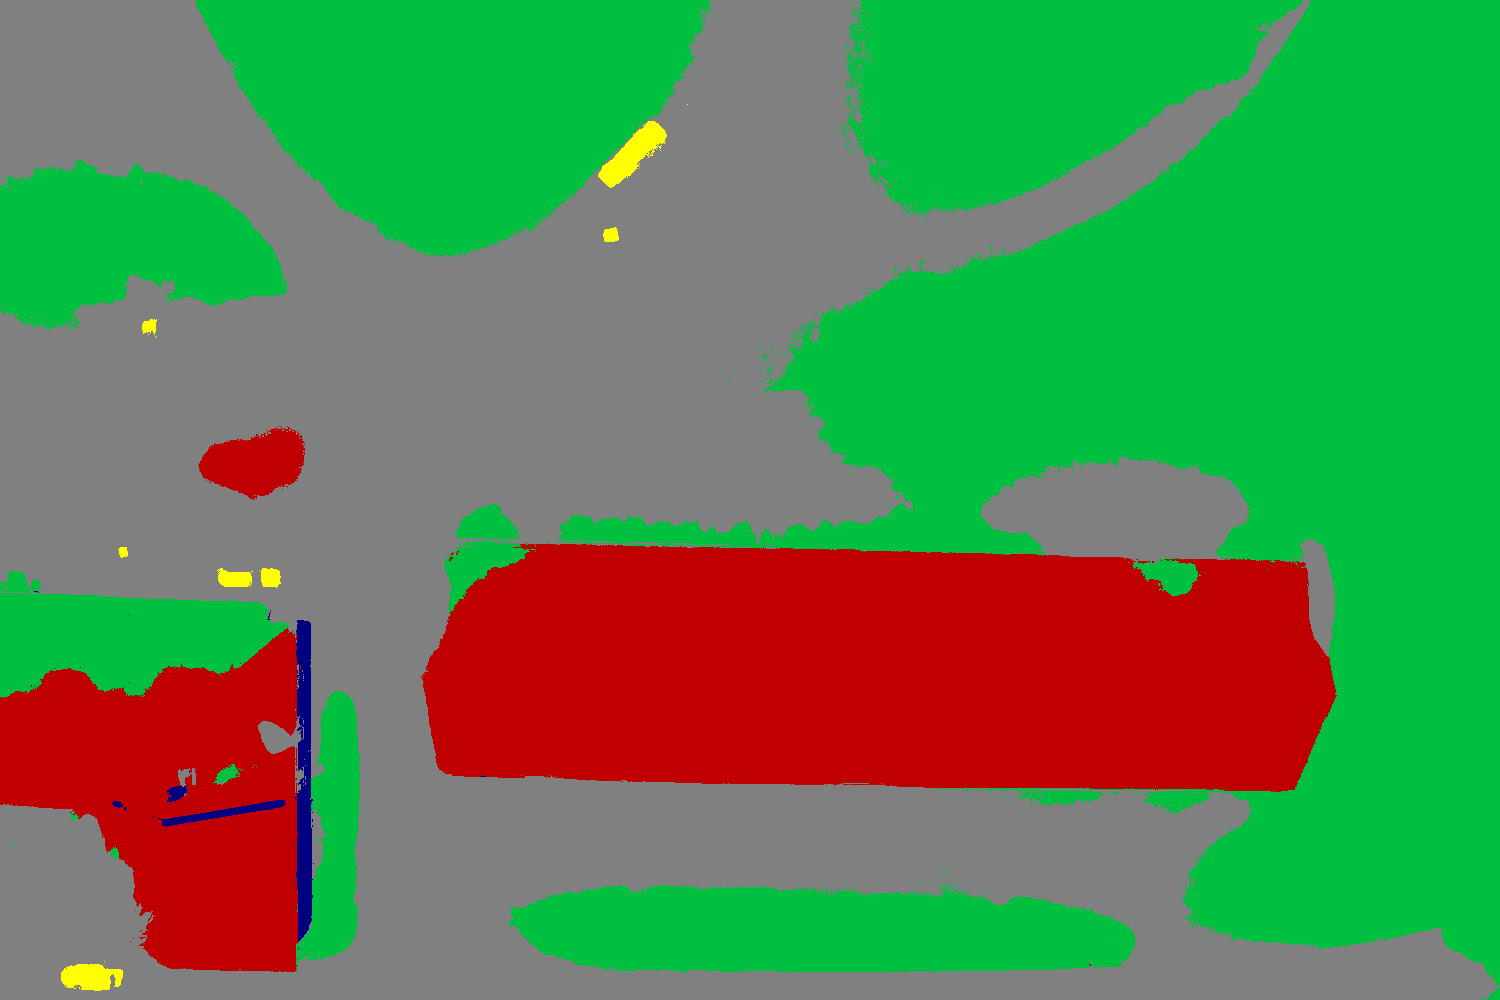
\includegraphics[width=1\linewidth]{fig/segmentation/DSC00958_manual.png}

\end{subfigure}
\begin{subfigure}{0.32\columnwidth}
  \centering
  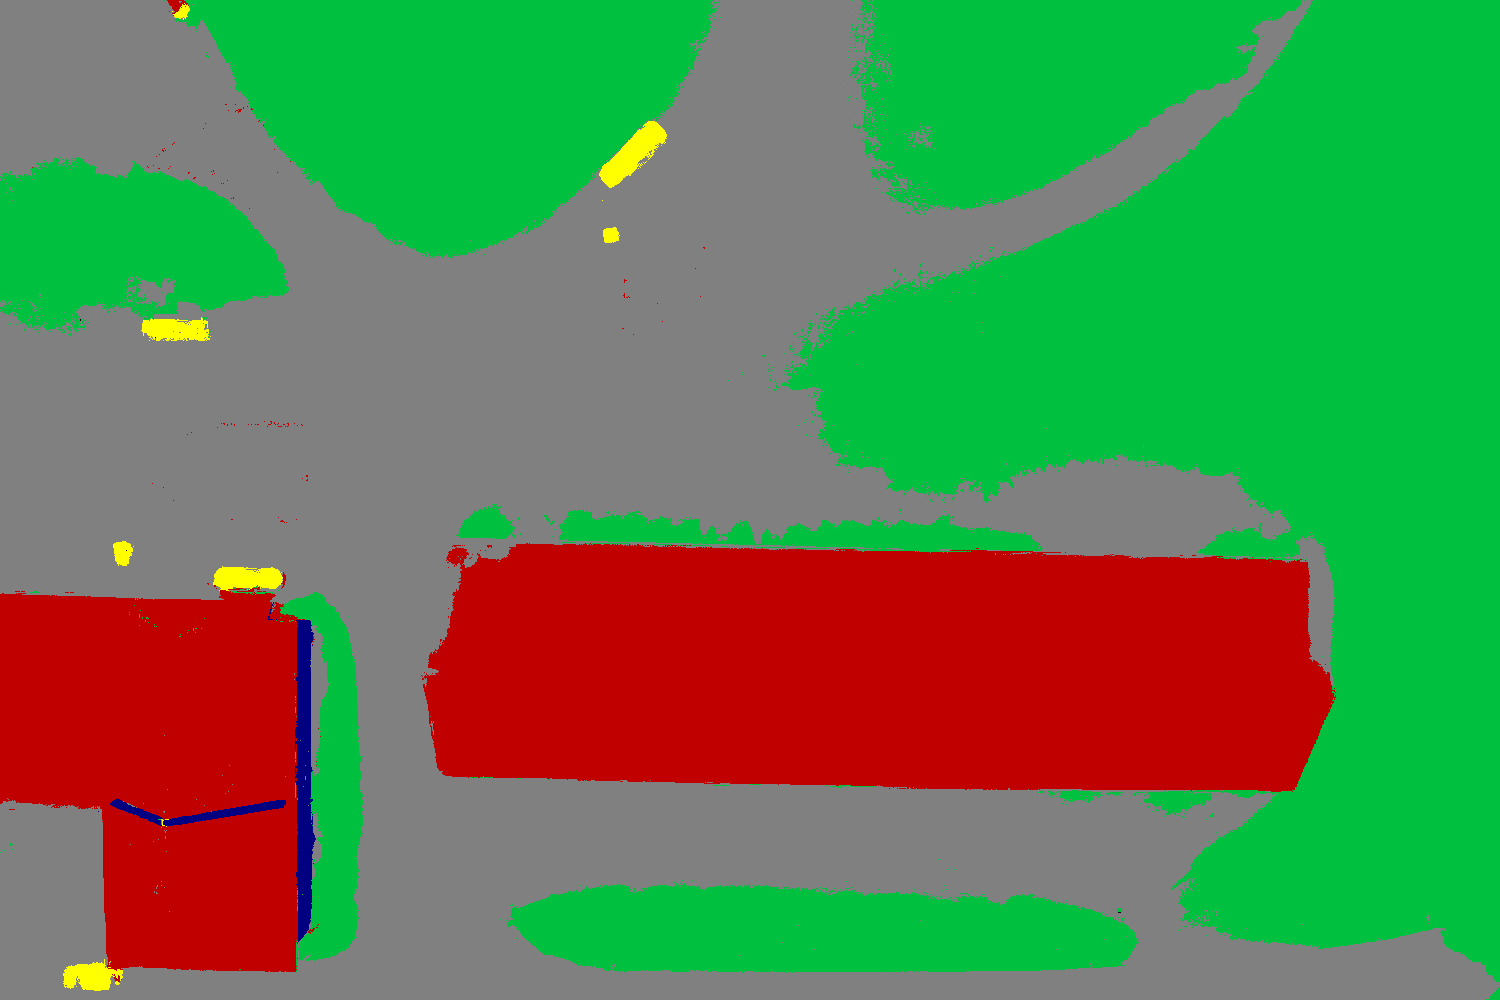
\includegraphics[width=1\linewidth]{fig/segmentation/DSC00958_auto.png}

\end{subfigure}
%\vspace{-0.5\baselineskip}

\begin{subfigure}{0.32\columnwidth}
  \centering
  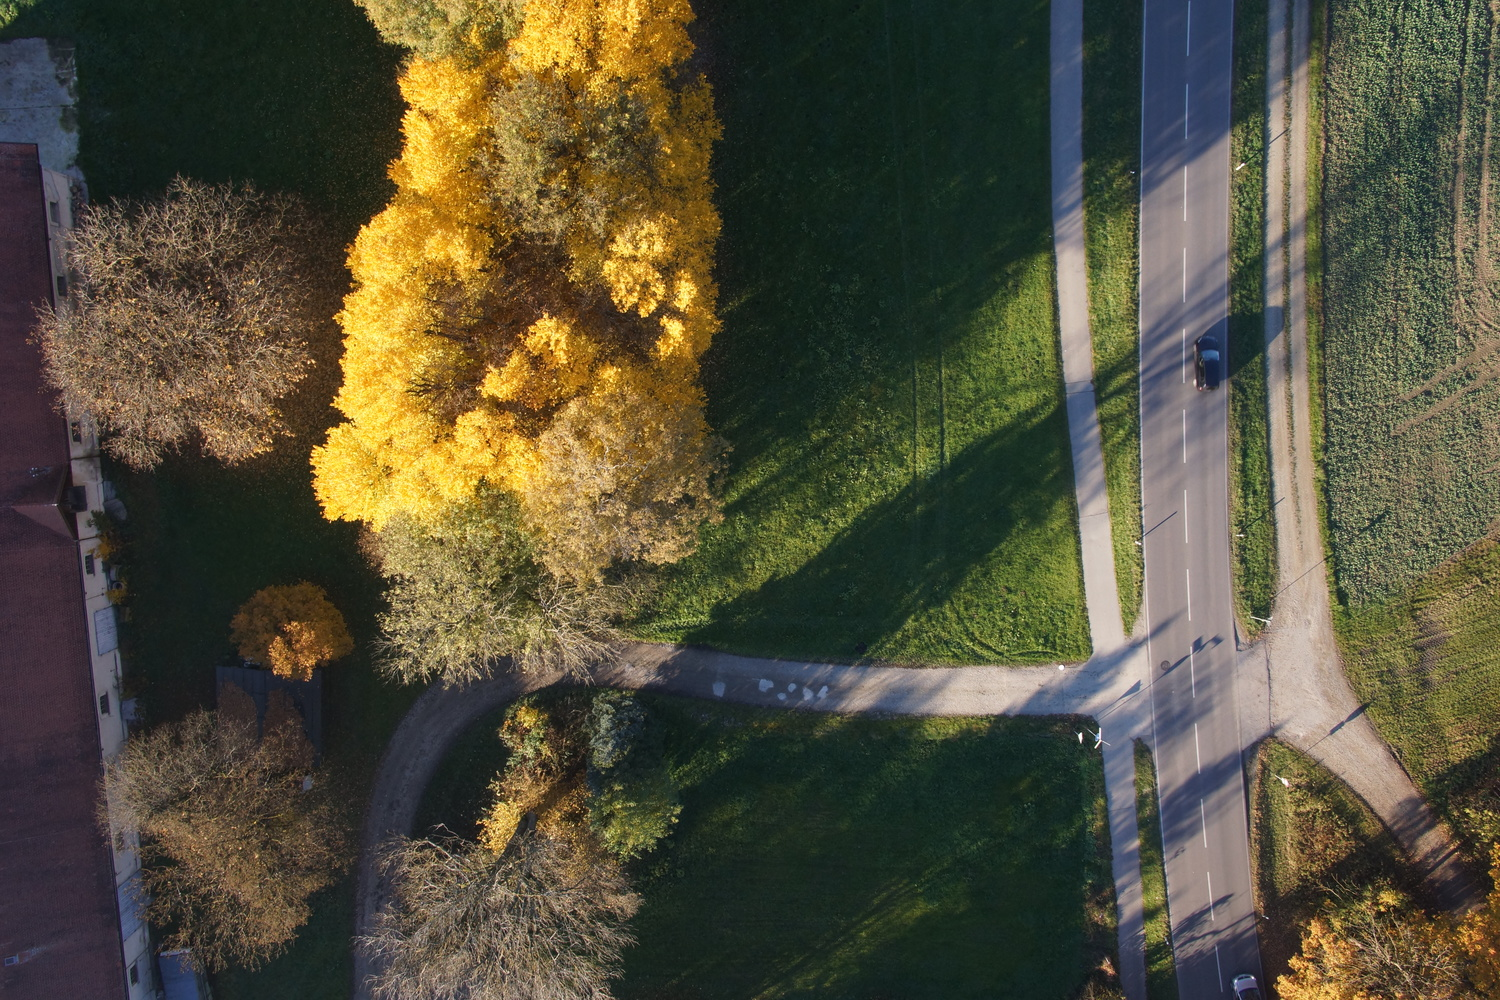
\includegraphics[width=1\linewidth]{fig/segmentation/DSC00991.JPG}

\end{subfigure}
\begin{subfigure}{0.32\columnwidth}
  \centering
  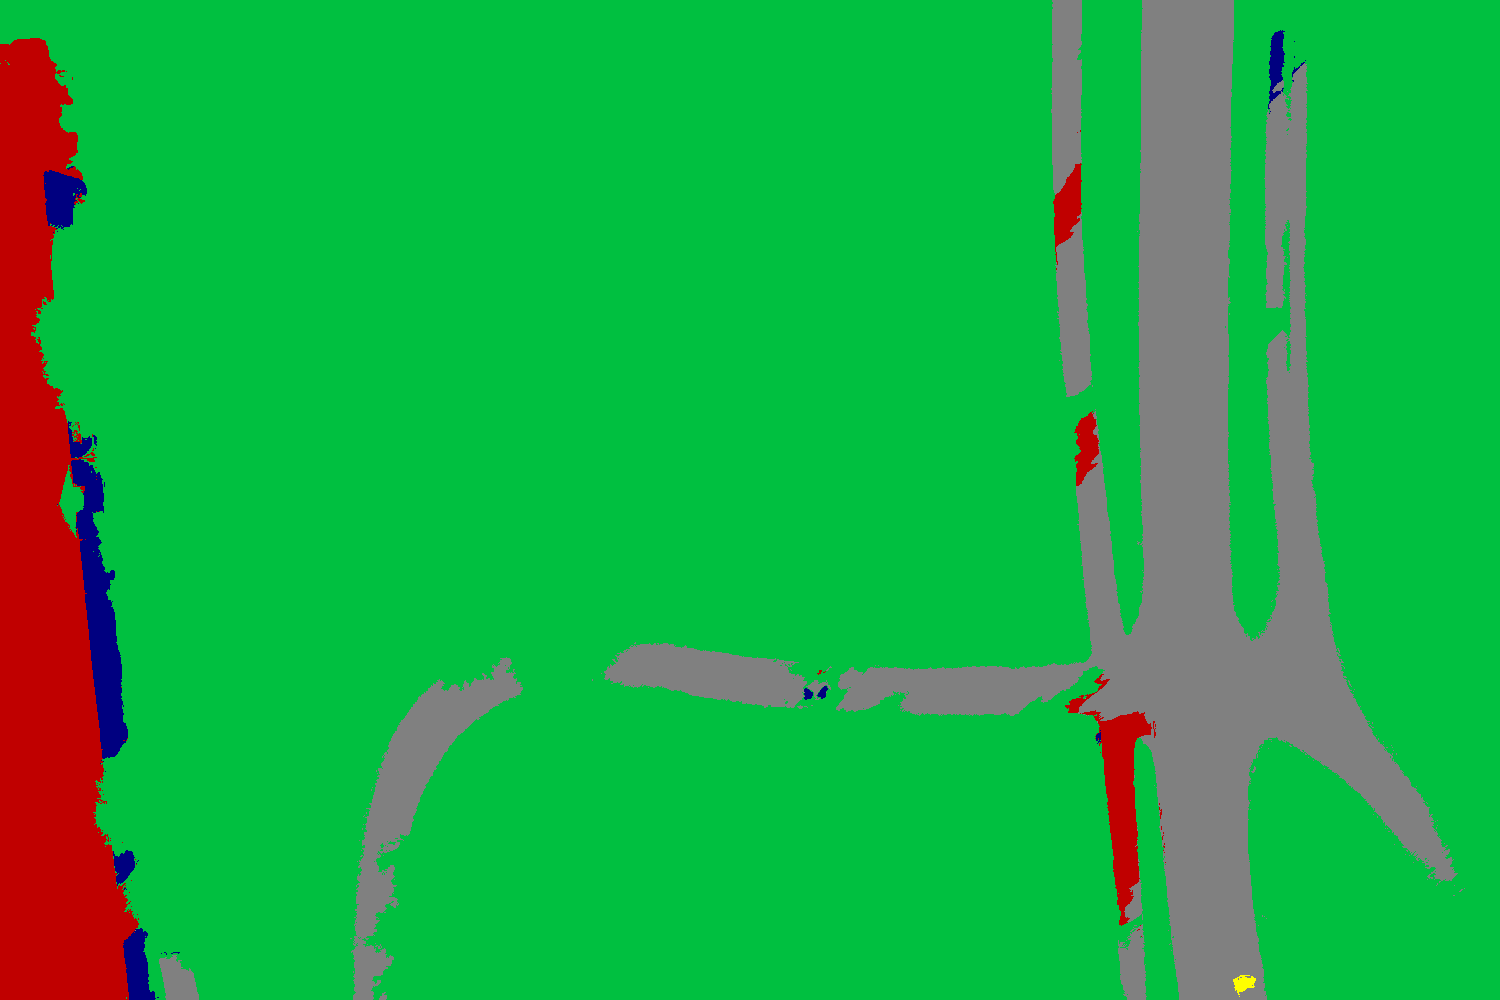
\includegraphics[width=1\linewidth]{fig/segmentation/DSC00991_manual.png}

\end{subfigure}
\begin{subfigure}{0.32\columnwidth}
  \centering
  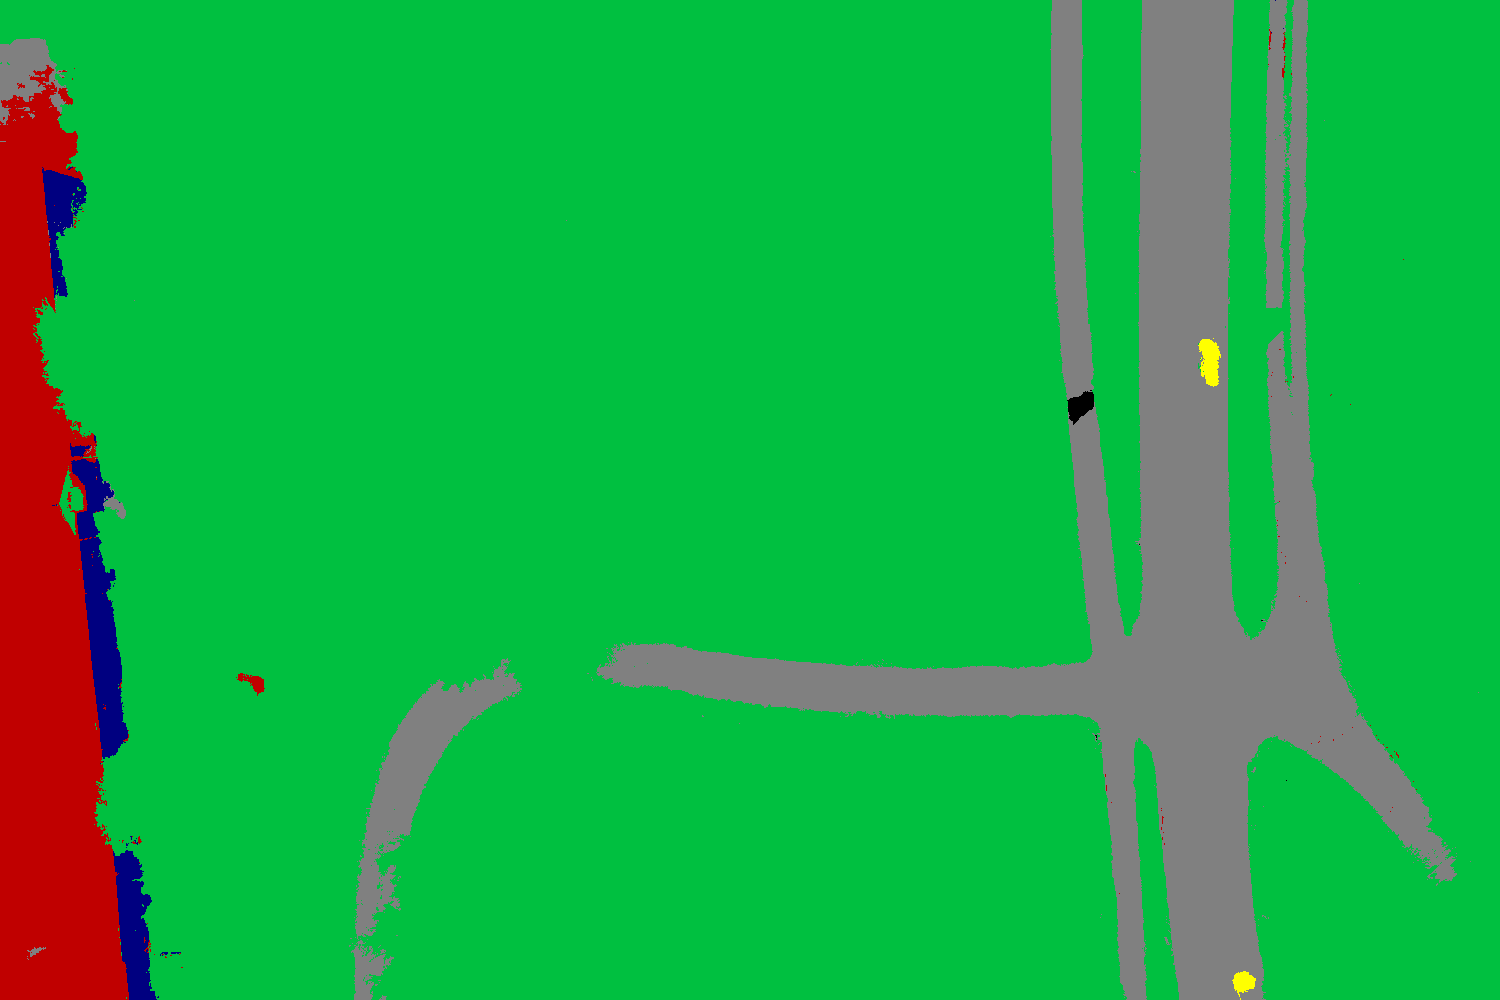
\includegraphics[width=1\linewidth]{fig/segmentation/DSC00991_auto.png}
\end{subfigure}

%\vspace{-0.5\baselineskip}

\begin{subfigure}{0.32\columnwidth}
  \centering
  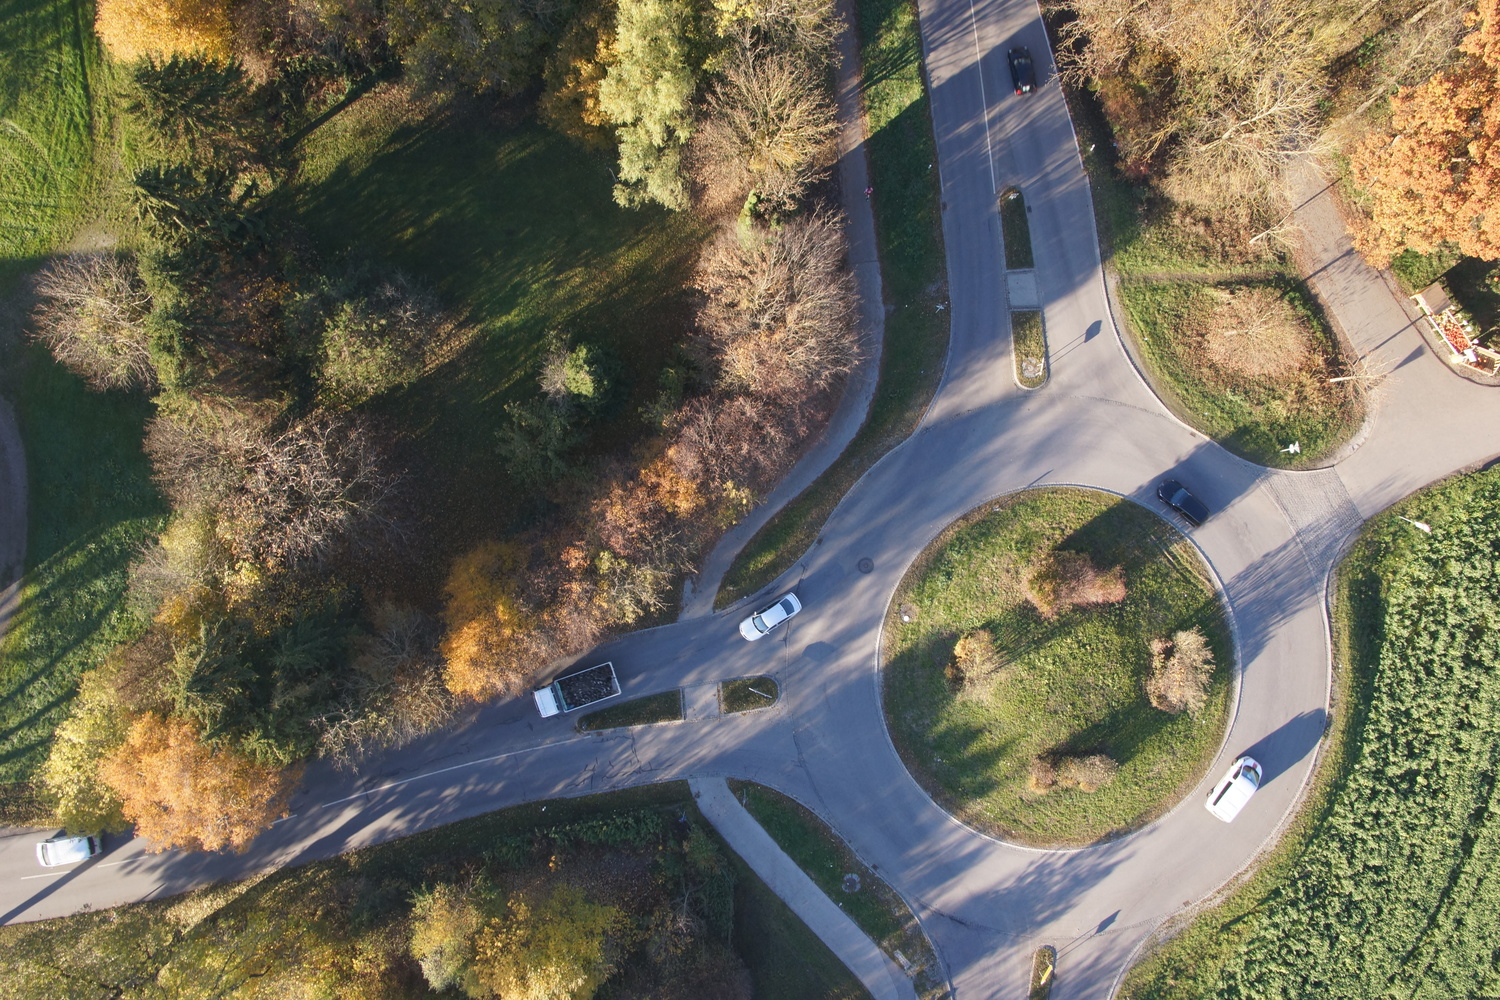
\includegraphics[width=1\linewidth]{fig/segmentation/DSC01001.JPG}

  \caption{}
\end{subfigure}
\begin{subfigure}{0.32\columnwidth}
  \centering
  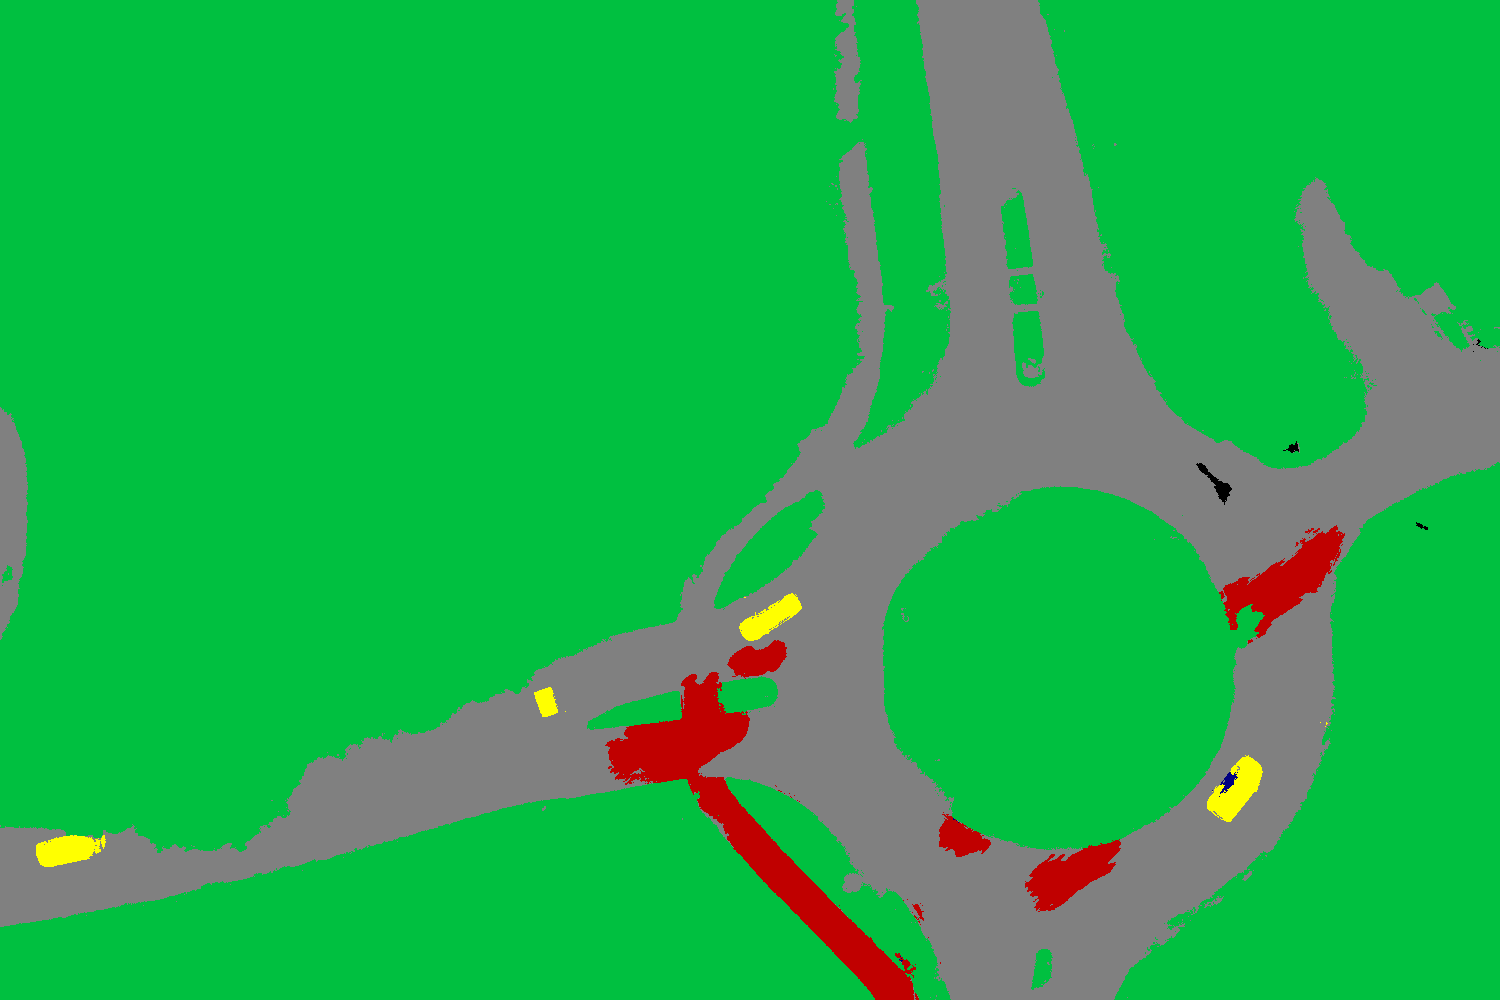
\includegraphics[width=1\linewidth]{fig/segmentation/DSC01001_manual.png}
 
  \caption{}
\end{subfigure}
\begin{subfigure}{0.32\columnwidth}
  \centering
  \includegraphics[width=1\linewidth]{fig/segmentation/DSC01001_auto.png}
  
  \caption{}
\end{subfigure}
\caption{Comparison of predictions on \textbf{Area 2}. (a) original UAV images, (b) predictions using 23 manually labeled frames from \textbf{Area 1} as training data, (c) predictions using 72 automatically labeled frames from \textbf{Area 1} as training data.}
\label{fig:area2}
\end{figure}

% \subsection{Building classification based on OSM footprint}

% \begin{figure}[htb]
% \begin{minipage}[b]{0.32\linewidth}
%   \centering
%   \centerline{\epsfig{figure=fig/512_rgb.png,width=2.8cm}}
%   \centerline{(a) }
% \end{minipage}
% \begin{minipage}[b]{0.32\linewidth}
%   \centering
%   \centerline{\epsfig{figure=fig/512_osm.png,width=2.8cm}}
%   \centerline{(b) }
% \end{minipage}
% \hfill
% \begin{minipage}[b]{0.32\linewidth}
%   \centering
%   \centerline{\epsfig{figure=fig/512_osm.png,width=2.8cm}}
%   \centerline{(c) }
% \end{minipage}
% \hfill
% \caption{Comparison of oblique aerial imagery and oblique UAV imagery. (a) is the UAV image, (b) and (c) show the corresponding region in the left-view and right-view aerial images}
% \label{fig:3k_uav}
% \end{figure}

% \begin{table}[htb]
%   \centering
%   \caption{Accuracy comparison of baseline methods and proposed method of Potsdam dataset.}
%     \begin{tabular}{ccccc}
%     \toprule
%     \textbf{Method} & \textbf{Ground} & \textbf{Building} & \textbf{Low Veg} & \textbf{Tree} \\
%     %Define if appropriate
          
%     \midrule
%     OSM     & - & 92.0 & - & -  \\
%     FCN  & 87.1  & 91.8  & 75.2  & 86.1\\
%     Deeplab     & 88.5  & 93.3& 73.9 & 86.9  \\
%     Bayesian-CRF  & - & 95.7 & - & -  \\
%     \bottomrule
%     \end{tabular}%
%   \label{tab:error_h}%
% \end{table}%
\section{automatic image annotation via label propagation from OSM footprints to aerial imagery}
\label{sec:experiment2}
In the last section, we have demonstrated the feasibility of automatic image annotating via label propagation, yet manual labeling of source images is still required. In this section, we leverage various remote sensing data for fully automatic annotating. In particular, we propagate OSM footprints to aerial imagery as weak annotations for buildings, and exploit geometric and radiometric information for multi-class image annotation. The experiment is implemented on the widely used Vaihingen dataset.

\subsection{Data Description}
The Vaihingen dataset was %initially designed for the 2D Semantic Labeling Test Project of ISPRS. 
provided by the German Association of Photogrammetry and Remote Sensing (DGPF) \cite{Cramer2010TheDO}. The images were captured in the summer of 2008 over Vaihingen, a medium-size village in Germany. The survey site is characterized by various buildings, including small detached houses, traditional buildings with complex shapes and high-rising buildings surrounded by trees. 

Image data used for this experiment includes 33 patches of true orthophoto (TOP) with a GSD of 9cm, each accompanied by a corresponding DSM with the same spatial resolution. The orthophotos were generated by Trimble INPHO OrthoVista as 8 bit TIFF files with three bands, i.e., near infrared, red and green bands. As the relative height above the ground is more interesting for our experiment rather than the absolute elevation, we generated heightmaps for each TOP by filtering and interpolating the ALS point cloud using LASTools\footnote{https://github.com/LAStools/LAStools}. The generated heightmaps have a grid size of 9cm, the same as the TOPs. 

There are 16 available ground-truth annotations of the TOPs, which are manually labeled into six categories, i.e., \textit{Impervious surfaces}, \textit{Building}, \textit{Low vegetation}, \textit{Tree}, \textit{Car} and \textit{Clutter}. In our implementation, we kept classes \textit{Building}, \textit{Low vegetation} and \textit{Tree}, and merged the rest categories (\textit{Impervious surfaces}, \textit{Car} and \textit{Clutter}) into a new category \textit{Ground}. Corresponding color coding is illustrated in Figure \ref{fig:colorbar_vai}. We selected twelve labeled TOPs (areas: 1, 3, 5, 7, 11, 15, 21, 26, 28, 32, 34 and 37) for training and the rest four labeled TOPs (areas: 13, 17, 23 and 30) for testing.
\begin{figure}[htb]
    \centering
\begin{subfigure}{0.8\columnwidth}
  \centering
  \includegraphics[width=1\linewidth]{fig/vai/colorbar_vai.JPG}
\end{subfigure} 
\caption{Color coding used for Vaihingen dataset}
       \label{fig:colorbar_vai}
\end{figure} 

The OSM footprint data used in experiments was downloaded on 21 May, 2018. Despite the large time offset compared with imagery data, the OSM footprints still have sufficient completeness in most areas. According to manual inspection, the position accuracy of OSM footprints ranges from a few decimeters in inner city to several meters in rural areas.
% The footprints contain only the planar coordinates of building footprints but no height information.  

\subsection{Automatic Image Annotating}
\subsubsection{Pixel Unary Potentials}
The pixel unary potential is derived from the OSM footprints data only. More formally, let $I$ denote the set of pixels in TOP and $\mathcal{L}$ denote the set of $K$ pre-defined labels. In our case, $K=4$, $\mathcal{L}= \big\{\textit{Building}, \textit{Low vegetation}, \textit{Tree}, \textit{Ground}\big\}$. Projecting OSM building footprints into a TOP image, the corresponding projection area is denoted by $I_b\left(I_b \subseteq I\right)$ and a degree of belief for the OSM footprints is denoted by $p$. Let $l_b$ denote the label index of class \textit{Building}, $P\left(x_i\right)$ encodes the prior belief of a pixel $i$ ($i\in I$) taking the label $x_i \left(x_i \in \mathcal{L}\right)$, which is defined as:

\begin{equation}
\label{eq:8}
\begin{aligned}
\forall i\in I_b, P\left(x_i\right)=\left\{
\begin{array}{lcl}
p & & {x_i = l_b}\\
\frac{\left(1-p\right)}{K-1} & & {x_i \neq l_b}
\end{array} \right.
\\
\forall i \notin I_b, P\left(x_i\right)=\left\{
\begin{array}{lcl}
1-p & & {x_i = l_b}\\
\frac{p}{K-1} & & {x_i \neq l_b}
\end{array} \right.
\end{aligned}
\end{equation}

Afterwards, the prior label assignment probability is updated via Bayesian inference given additional evidence. In this experiment, we exploited the height and NDVI values as additional evidence, denoted by $H$ and $N$ respectively (the evidence set $\mathbf{O}$ in Equation \ref{eq:3} is namely \big\{H, N\big\}). Particularly, the height value is extracted from the heightmap and the NDVI is calculated based on image radiometric information using following formula: 
\begin{equation}
\label{eq:9}
\begin{array}{lcl}
NDVI = \frac {(NIR-Red)}{(NIR+Red)}\\
\end{array}
\end{equation}
where NIR and Red are the gray values of the TOP tiff files.

Let $P\left(H\mid \mathbf{x}\right)$ and $P\left(N\mid \mathbf{x}\right)$ denote the likelihoods of height and NDVI value for given class $\mathbf{x}$, which are empirically defined based on image statistics. In our settings, we model the likelihood function as a normal distribution. In complicated cases, e.g., the pre-defined class \textit{Tree} includes bushes and tall trees which have different distribution on height, we then model the likelihood function as a weighted sum of normal distributions, i.e., $f(H;\mu ,\sigma ^{2}) = \sum \omega_i\frac {1}{\sqrt {2\pi \sigma_i ^{2}}}e^{-\frac {(H-\mu_i )^{2}}{2\sigma_i ^{2}}}$. A visualization of the likelihood functions is illustrated in Figure \ref{fig:vai_distrib}, and the parameter settings are listed in Table \ref{tab:vai_para_h} and \ref{tab:vai_para_ndvi}. In particular, the lower bounds for the height of \textit{Tree} and \textit{Building} were set as 0.5m and 2m respectively. For the sake of simplification, we assume \textit{Tree} and \textit{Low Veg}, \textit{Ground} and \textit{Building} have the same likelihood functions for NDVI. Considering the fact that the vegetation NDVI has relatively lower value in shaded areas, the likelihood function for vegetation NDVI is composed of two normal distributions representing the NDVI in normal cases and in shaded areas. Provided observations on height and NDVI, the posterior distribution $P\left(\mathbf{x} \mid H, N\right)$, can be calculated based on Equations \ref{eq:2} and \ref{eq:3}.

\begin{figure}[htb]
    \centering
       \begin{subfigure}{0.48\columnwidth}
	       \centering
           \includegraphics[width=\linewidth]{fig/vai/vai_height}	
       \end{subfigure}
       ~
       \begin{subfigure}{0.48\columnwidth}
	       \centering
			\includegraphics[width=\linewidth]{fig/vai/vai_ndvi}	
       \end{subfigure}       
       \caption{Probability distributions of height and NDVI for Vaihingen dataset.}
       \label{fig:vai_distrib}
\end{figure}


\begin{table}[htbp]
  \centering
  \caption{Parameter settings of probability distribution functions for height, Vaihingen Dataset.}
    \begin{tabular}{c|c|c|c|c|c}
    \hline
    \textbf{Parameter} & \textbf{Ground} & \textbf{Building} & \textbf{Low Veg} & \multicolumn{2}{c}{\textbf{Tree}} \\
    %Define if appropriate
          
    \hline
    $\omega$     & 2     & 1     & 2     & 0.4   & 0.5 \\
    
    $\mu$     & 0     & 7.5   & 0     & 2.5   & 5 \\
    
    $\sigma$ & 0.5   & 3.5   & 1     & 1.5   & 4 \\
    \hline
    \end{tabular}%
  \label{tab:vai_para_h}%
\end{table}%

\begin{table}[htbp]
  \centering
  \caption{Parameter settings of probability distribution functions for NDVI, Vaihingen Dataset.}
    \begin{tabular}{c|c|c|c}
    \hline
    \textbf{Parameter} & \textbf{Ground}, \textbf{Building} & \multicolumn{2}{c}{\textbf{Low Veg}, \textbf{Tree}} \\
    %Define if appropriate
          
    \hline
    $\omega$     & 1       & 0.9   & 0.1 \\
    
    $\mu$     & -0.1        & 0.5   & 0.1 \\
    
    $\sigma$ & 0.2      & 0.1   & 0.05 \\
    \hline
    \end{tabular}%
  \label{tab:vai_para_ndvi}%
\end{table}%

Intuitively, the height evidence helps to distinguish high objects like buildings and trees from low objects like low vegetation and the ground, while the NDVI evidence can effectively differentiate low vegetation and trees from non-vegetation.

\subsubsection{Inference}
A few examples of the inferred annotations are depicted in Figure \ref{fig:vai_infer}. The source data required for inference is listed in columns (a) - (c): (a) true orthophotos with three bands: near infrared, red and green, (b) corresponding heightmaps, (c) building masks projected from OSM footprints. After inference using our Bayesian-CRF graphical model, the generated image annotations are depicted in column (d), and the manually labeled ground-truth data is listed in column (e). It can be seen that the automatically generated annotations have high similarity with manual annotations in general. However, in dark or shaded areas, there are a few errors in categories \textit{Low Vegetation} and \textit{Tree}. This is because the NDVI value cannot well distinguish the vegetation from the ground in shaded areas. 


\begin{figure*}[htb]
\begin{subfigure}{0.19\textwidth}
  \centering
  \includegraphics[width=1\linewidth]{fig/vai/1_irg.JPG}
  
\end{subfigure}\vspace{1mm}
\begin{subfigure}{0.19\textwidth}
  \centering
  \includegraphics[width=1\linewidth]{fig/vai/1_hm.jpg}
\end{subfigure}
\begin{subfigure}{0.19\textwidth}
  \centering
  \includegraphics[width=1\linewidth]{fig/vai/1_osm.jpg}
\end{subfigure}
\begin{subfigure}{0.19\textwidth}
  \centering
  \includegraphics[width=1\linewidth]{fig/vai/1_anno.png}
\end{subfigure}
\begin{subfigure}{0.19\textwidth}
  \centering
  \includegraphics[width=1\linewidth]{fig/vai/1_gt.png}
\end{subfigure}

% \begin{subfigure}{0.19\textwidth}
%   \centering
%   \includegraphics[width=1\linewidth]{fig/vai/3_irg.JPG}
% \end{subfigure}\vspace{1mm}
% \begin{subfigure}{0.19\textwidth}
%   \centering
%   \includegraphics[width=1\linewidth]{fig/vai/3_hm.jpg}
% \end{subfigure}
% \begin{subfigure}{0.19\textwidth}
%   \centering
%   \includegraphics[width=1\linewidth]{fig/vai/3_osm.jpg}
% \end{subfigure}
% \begin{subfigure}{0.19\textwidth}
%   \centering
%   \includegraphics[width=1\linewidth]{fig/vai/3_anno.png}
% \end{subfigure}
% \begin{subfigure}{0.19\textwidth}
%   \centering
%   \includegraphics[width=1\linewidth]{fig/vai/3_gt.png}
% \end{subfigure}

\begin{subfigure}{0.19\textwidth}
  \centering
  \includegraphics[width=1\linewidth]{fig/vai/5_irg.JPG}
\end{subfigure}\vspace{1mm}
\begin{subfigure}{0.19\textwidth}
  \centering
  \includegraphics[width=1\linewidth]{fig/vai/5_hm.jpg}
\end{subfigure}
\begin{subfigure}{0.19\textwidth}
  \centering
  \includegraphics[width=1\linewidth]{fig/vai/5_osm.jpg}
\end{subfigure}
\begin{subfigure}{0.19\textwidth}
  \centering
  \includegraphics[width=1\linewidth]{fig/vai/5_anno.png}
\end{subfigure}
\begin{subfigure}{0.19\textwidth}
  \centering
  \includegraphics[width=1\linewidth]{fig/vai/5_gt.png}
\end{subfigure}

% \begin{subfigure}{0.19\textwidth}
%   \centering
%   \includegraphics[width=1\linewidth]{fig/vai/7_irg.JPG}
% \end{subfigure}\vspace{1mm}
% \begin{subfigure}{0.19\textwidth}
%   \centering
%   \includegraphics[width=1\linewidth]{fig/vai/7_hm.jpg}
% \end{subfigure}
% \begin{subfigure}{0.19\textwidth}
%   \centering
%   \includegraphics[width=1\linewidth]{fig/vai/7_gt.png}
% \end{subfigure}
% \begin{subfigure}{0.19\textwidth}
%   \centering
%   \includegraphics[width=1\linewidth]{fig/vai/7_osm.jpg}
% \end{subfigure}
% \begin{subfigure}{0.19\textwidth}
%   \centering
%   \includegraphics[width=1\linewidth]{fig/vai/7_anno.png}
% \end{subfigure}

\begin{subfigure}{0.19\textwidth}
  \centering
  \includegraphics[width=1\linewidth]{fig/vai/26_irg.JPG}
\end{subfigure}\vspace{1mm}
\begin{subfigure}{0.19\textwidth}
  \centering
  \includegraphics[width=1\linewidth]{fig/vai/26_hm.jpg}
\end{subfigure}
\begin{subfigure}{0.19\textwidth}
  \centering
  \includegraphics[width=1\linewidth]{fig/vai/26_osm.jpg}
\end{subfigure}
\begin{subfigure}{0.19\textwidth}
  \centering
  \includegraphics[width=1\linewidth]{fig/vai/26_anno.png}
\end{subfigure}
\begin{subfigure}{0.19\textwidth}
  \centering
  \includegraphics[width=1\linewidth]{fig/vai/26_gt.png}
\end{subfigure}

\begin{subfigure}{0.19\textwidth}
  \centering
  \includegraphics[width=1\linewidth]{fig/vai/32_irg.JPG}
\end{subfigure}\vspace{1mm}
\begin{subfigure}{0.19\textwidth}
  \centering
  \includegraphics[width=1\linewidth]{fig/vai/32_hm.jpg}
\end{subfigure}
\begin{subfigure}{0.19\textwidth}
  \centering
  \includegraphics[width=1\linewidth]{fig/vai/32_osm.jpg}
\end{subfigure}
\begin{subfigure}{0.19\textwidth}
  \centering
  \includegraphics[width=1\linewidth]{fig/vai/32_anno.png}
\end{subfigure}
\begin{subfigure}{0.19\textwidth}
  \centering
  \includegraphics[width=1\linewidth]{fig/vai/32_gt.png}
\end{subfigure}

\begin{subfigure}{0.19\textwidth}
  \centering
  \includegraphics[width=1\linewidth]{fig/vai/37_irg.JPG}
  \caption{}
\end{subfigure}\vspace{1mm}
\begin{subfigure}{0.19\textwidth}
  \centering
  \includegraphics[width=1\linewidth]{fig/vai/37_hm.jpg}
  \caption{}
\end{subfigure}
\begin{subfigure}{0.19\textwidth}
  \centering
  \includegraphics[width=1\linewidth]{fig/vai/37_osm.jpg}
  \caption{}
\end{subfigure}
\begin{subfigure}{0.19\textwidth}
  \centering
  \includegraphics[width=1\linewidth]{fig/vai/37_anno.png}
  \caption{}
\end{subfigure}
\begin{subfigure}{0.19\textwidth}
  \centering
  \includegraphics[width=1\linewidth]{fig/vai/37_gt.png}
  \caption{}
\end{subfigure}
\caption{Comparison of manual annotations and inferred annotations. (a) true orthophoto, (b) corresponding heightmap, (c) building mask projected from OSM building footprint, (d) automatically inferred image annotations, (e) manually labeled ground-truth.}
%\caption{Predictions of No.30 tile in Vaihingen dataset, where (a) is the original true orthophoto, (b) is the ground truth, (c) is the building mask created from OSM building footprint and (d) depicts the inferred annotation}
\label{fig:vai_infer}
\end{figure*}

\subsection{Analysis of Inferred Annotations}
Manual image annotating interprets the scene merely based on image information, thus the accuracy is usually lower at areas with low brightness and contrast. In comparison, our method jointly utilizes the complimentary radiometric and geometric information, which contributes to higher semantic accuracy in such situations. Additionally, the inferred annotations inherently conform to image gradients and therefore have higher shape accuracy for irregular objects.

\subsubsection{Comparison With Manual Annotations}
Manual image annotating often suffers from the existence of shadow, in such cases, our method can achieve higher semantic accuracy as it also takes height information into consideration. A few examples are illustrated in Figure \ref{fig:vai_comp_manual}. From left to right in each row, (a)-(e) are snapshots from Google Maps, true orthophotos, manually labeled ground-truth data, corresponding heightmaps and automatically inferred annotations, respectively. Building areas to be noted are highlighted in red. More specifically, figures in the first row show a building which is visible in Google Maps but partly hidden in shadows in the true orthophoto, therefore it was wrongly labeled as ground in manual annotation. However, with the help of the height evidence, our method labeled the building correctly. A similar example is shown in the second row, where the ground was wrongly labeled as building in manual annotation but correctly labeled by our method. The third row presents an example for shape accuracy of buildings, demonstrating that the inferred annotation is more accurate at building boundaries than manual annotation.


\begin{figure}[H]
\begin{subfigure}{0.19\columnwidth}
  \centering
  \includegraphics[width=1\linewidth]{fig/comp_manual/building1_google.jpg}
\end{subfigure}
\begin{subfigure}{0.19\columnwidth}
  \centering
  \includegraphics[width=1\linewidth]{fig/comp_manual/building_1_rgb2.png}  
\end{subfigure}\vspace{1mm}
\begin{subfigure}{0.19\columnwidth}
  \centering
\begin{tikzpicture}
    \node[inner sep=0pt] (ima) at (0,0) {\includegraphics[width=1\columnwidth]{fig/comp_manual/building_1_gt2.png}};
     %\begin{scope}[x={(ima.south east)},y={(ima.north west)}]
         \draw[red, dashed, ultra thick,rounded corners] (-0.9,0.7) rectangle (-0.2,-0.3);
     %\end{scope}    
 \end{tikzpicture}
\end{subfigure}
\begin{subfigure}{0.19\columnwidth}
  \centering
  \begin{tikzpicture}
    \node[inner sep=0pt] (ima) at (0,0) {\includegraphics[width=1\columnwidth]{fig/comp_manual/building_1_hm2_ori.png}};
     %\begin{scope}[x={(ima.south east)},y={(ima.north west)}]
         %\draw[red, ultra thick,rounded corners] (-0.7,0.7) rectangle (0.2,-0.5);
     %\end{scope}    
 \end{tikzpicture}
\end{subfigure}
\begin{subfigure}{0.19\columnwidth}
  \centering
\begin{tikzpicture}
    \node[inner sep=0pt] (ima) at (0,0) {\includegraphics[width=1\columnwidth]{fig/comp_manual/building_1_anno2.png}};
     %\begin{scope}[x={(ima.south east)},y={(ima.north west)}]
         \draw[red, ultra thick,rounded corners] (-0.9,0.7) rectangle (-0.2,-0.3);
     %\end{scope}    
 \end{tikzpicture}
\end{subfigure}


\begin{subfigure}{0.19\columnwidth}
  \centering
  \includegraphics[width=1\linewidth]{fig/comp_manual/building28_google.jpg}
\end{subfigure}
\begin{subfigure}{0.19\columnwidth}
  \centering
  \includegraphics[width=1\linewidth]{fig/comp_manual/building_28_rgb.png}  
\end{subfigure}\vspace{1mm}
\begin{subfigure}{0.19\columnwidth}
  \centering
\begin{tikzpicture}
    \node[inner sep=0pt] (ima) at (0,0) {\includegraphics[width=1\columnwidth]{fig/comp_manual/building_28_gt.png}};
     %\begin{scope}[x={(ima.south east)},y={(ima.north west)}]
         \draw[red, dashed, ultra thick,rounded corners] (-0.8,0.7) rectangle (0.3,-0.8);
     %\end{scope}    
 \end{tikzpicture}
\end{subfigure}
\begin{subfigure}{0.19\columnwidth}
  \centering
  \begin{tikzpicture}
    \node[inner sep=0pt] (ima) at (0,0) {\includegraphics[width=1\columnwidth]{fig/comp_manual/building_28_hm_ori.png}};
     %\begin{scope}[x={(ima.south east)},y={(ima.north west)}]
         %\draw[red, ultra thick,rounded corners] (-0.8,0.7) rectangle (0.3,-0.8);
     %\end{scope}    
 \end{tikzpicture}
\end{subfigure}
\begin{subfigure}{0.19\columnwidth}
  \centering
\begin{tikzpicture}
    \node[inner sep=0pt] (ima) at (0,0) {\includegraphics[width=1\columnwidth]{fig/comp_manual/building_28_anno.png}};
     %\begin{scope}[x={(ima.south east)},y={(ima.north west)}]
         \draw[red, ultra thick,rounded corners] (-0.8,0.7) rectangle (0.3,-0.8);
     %\end{scope}    
 \end{tikzpicture}
\end{subfigure}

\begin{subfigure}{0.19\columnwidth}
  \centering
  \includegraphics[width=1\linewidth]{fig/comp_manual/building_1_google.jpg}
  \caption{}
\end{subfigure}
\begin{subfigure}{0.19\columnwidth}
  \centering
  \includegraphics[width=1\linewidth]{fig/comp_manual/building_1_rgb.png}  
 \caption{} 
\end{subfigure}\vspace{1mm}
\begin{subfigure}{0.19\columnwidth}
  \centering
\begin{tikzpicture}
    \node[inner sep=0pt] (ima) at (0,0) {\includegraphics[width=1\columnwidth]{fig/comp_manual/building_1_gt.png}};
     %\begin{scope}[x={(ima.south east)},y={(ima.north west)}]
         \draw[red, dashed, ultra thick,rounded corners] (-0.2,0.1) rectangle (0.8,-0.8);
     %\end{scope}    
 \end{tikzpicture}
 \caption{}
\end{subfigure}
\begin{subfigure}{0.19\columnwidth}
  \centering
  \begin{tikzpicture}
    \node[inner sep=0pt] (ima) at (0,0) {\includegraphics[width=1\columnwidth]{fig/comp_manual/building_1_hm.png}};
     %\begin{scope}[x={(ima.south east)},y={(ima.north west)}]
         %\draw[red, ultra thick,rounded corners] (-0.2,0.1) rectangle (0.8,-0.8);
     %\end{scope}    
 \end{tikzpicture}
 \caption{}
\end{subfigure}
\begin{subfigure}{0.19\columnwidth}
  \centering
\begin{tikzpicture}
    \node[inner sep=0pt] (ima) at (0,0) {\includegraphics[width=1\columnwidth]{fig/comp_manual/building_1_anno.png}};
     %\begin{scope}[x={(ima.south east)},y={(ima.north west)}]
         \draw[red, ultra thick,rounded corners] (-0.2,0.1) rectangle (0.8,-0.8);
     %\end{scope}    
 \end{tikzpicture}
 \caption{}
\end{subfigure}






% \begin{subfigure}{0.24\columnwidth}
%   \centering
%   \includegraphics[width=1\linewidth]{fig/comp_manual/building_5_rgb.png}  
%   \caption{}
% \end{subfigure}\vspace{1mm}
% \begin{subfigure}{0.24\columnwidth}
%   \centering
%   \includegraphics[width=1\linewidth]{fig/comp_manual/building_5_hm.png}
%   \caption{}
% \end{subfigure}
% \begin{subfigure}{0.24\columnwidth}
%   \centering
%   \includegraphics[width=1\linewidth]{fig/comp_manual/building_5_gt.png}
%   \caption{}
% \end{subfigure}
% \begin{subfigure}{0.24\columnwidth}
%   \centering
%   \includegraphics[width=1\linewidth]{fig/comp_manual/building_5_anno.png}
%   \caption{}
% \end{subfigure}
\caption{Comparison of building accuracy between automatically inferred and manually labeled annotations. (a) snapshot from Google Maps, (b) true orthophotos, (c) manually labeled ground-truth data, (d) corresponding heightmaps, (e) automatically inferred annotations. Building areas to be noted are highlighted in red. Dashed lines indicate wrong labeling and solid lines indicate correct labeling.}
\label{fig:vai_comp_manual}
\end{figure}

The semantic accuracy of class \textit{Ground} is compared in Figure \ref{fig:vai_comp_manual_ground}. From left to right in each row, (a)-(c) are true orthophotos, manually labeled ground-truth data and automatically inferred annotations respectively. In the two scenes, although the bare ground nearby buildings or through the grassland can be easily recognized on orthophotos, precise annotating is still unpractical due to its irregular shape. Therefore many ground areas are roughly labeled or ignored, as highlighted by the red dashed boxes. By contrast, they are correctly labeled in the automatic annotations, as highlighted by the red solid boxes.  
\begin{figure}[H]
\begin{subfigure}{0.315\columnwidth}
  \centering
  \includegraphics[width=1\linewidth]{fig/comp_manual/15_rgb1_crop.jpg}  
  %\caption{}
\end{subfigure}\vspace{1mm}
~
\begin{subfigure}{0.315\columnwidth}
  \centering
   \begin{tikzpicture}
    \node[inner sep=0pt] (ima) at (0,0) {\includegraphics[width=1\columnwidth]{fig/comp_manual/15_gt1_crop.jpg}};
     \draw[red, dashed, ultra thick,rounded corners] (-1.3,1.35) rectangle (-0.3,0.9);
     \draw[red, dashed, ultra thick,rounded corners] (0.1,1.35) rectangle (1.2,-0.5);
 \end{tikzpicture}
\end{subfigure}
~
\begin{subfigure}{0.315\columnwidth}
  \centering
  \begin{tikzpicture}
    \node[inner sep=0pt] (ima) at (0,0) {\includegraphics[width=1\columnwidth]{fig/comp_manual/15_anno1_crop.jpg}};
     \draw[red, ultra thick,rounded corners] (-1.3,1.35) rectangle (-0.3,0.9);
     \draw[red, ultra thick,rounded corners] (0.1,1.35) rectangle (1.2,-0.5);
 \end{tikzpicture}
  %\caption{}
\end{subfigure}

\begin{subfigure}{0.315\columnwidth}
  \centering
  \includegraphics[width=1\linewidth]{fig/comp_manual/15_rgb2_crop.jpg}  
  \caption{}
\end{subfigure}\vspace{1mm}
~
\begin{subfigure}{0.315\columnwidth}
  \centering
  \begin{tikzpicture}
    \node[inner sep=0pt] (ima) at (0,0) {\includegraphics[width=1\columnwidth]{fig/comp_manual/15_gt2_crop.jpg}};
         \draw[red, dashed, ultra thick,rounded corners] (-1.3,0.7) rectangle (0.3,-0.8);
 \end{tikzpicture}
  \caption{}
\end{subfigure}
~
\begin{subfigure}{0.315\columnwidth}
  \centering
  \begin{tikzpicture}
    \node[inner sep=0pt] (ima) at (0,0) {\includegraphics[width=1\columnwidth]{fig/comp_manual/15_anno2_crop.jpg}};
         \draw[red, ultra thick,rounded corners] (-1.3,0.7) rectangle (0.3,-0.8);
 \end{tikzpicture}
  \caption{}
\end{subfigure}
\caption{Comparison of ground accuracy between automatically inferred and manually labeled annotations. (a) true orthophotos, (b) manually labeled ground-truth data, (c) automatically inferred annotations. Ground areas to be compared are highlighted in red. Dashed lines indicate wrong labeling and solid lines indicate correct labeling.}
\label{fig:vai_comp_manual_ground}
\end{figure}



On the other hand, the performance of our method is influenced by the accuracy of heightmaps. Inaccurate height information may lead to wrong labeling, especially when the image content is not distinguishable. For instance, grassland and bushes are labeled respectively as \textit{Low Vegetation} and \textit{Tree} in ground-truth annotations, however, the heightmap extracted from the DSM can not well preserve the small height difference between them and the NDVI evidence is not distinguishable either. This accounts for the wrong annotations for classes \textit{Low Vegetation} and \textit{Tree}, as shown in Figure \ref{fig:vai_comp_manual} and \ref{fig:vai_comp_manual_ground}. 


\subsubsection{Comparison with OSM building footprints}
Building annotations are originally derived from the up-to-date OSM data, which has about ten years time offset with the image data. The considerable temporal changes of building result in low semantic accuracy of the source labeling. Nevertheless, our method is able to generate building annotations with substantially improved accuracy based on additional evidence. Figure \ref{fig:vai_comp_osm} presents a comparison between OSM building footprints (left column) and inferred building annotations (right column), which are both overlaid on TOP. The highlighted areas in (a), (c) indicate the errors in OSM footprints caused by temporal changes of buildings, which, in contrast, are correctly labeled in the inferred annotations. Besides, OSM footprints usually have low position accuracy, especially in rural areas. As compared in (e), (f), the OSM building footprints have large shift in position while the inferred annotations have apparently higher position accuracy. Third, OSM footprints usually have simplified shapes as illustrated in (g), but the inferred annotations achieve high shape accuracy for buildings with complex structures.
% Even for the buildings which are partly covered or occluded by vegetations, the inference can still result in accurate class boundaries.  


\begin{figure}[H]
 \begin{subfigure}{0.485\columnwidth}
   \centering
\begin{tikzpicture}
    \node[inner sep=0pt] (ima) at (0,0) {\includegraphics[width=1\columnwidth]{fig/comp_osm/37_osm_lay.png}};
     %\begin{scope}[x={(ima.south east)},y={(ima.north west)}]
         \draw[yellow, dashed, very thick,rounded corners] (-0.5,0.1) rectangle (2,0.9);
         %\draw[yellow, dashed, very thick,rounded corners] (0.6,0.1) rectangle (2,1);
         \draw[yellow, dashed, very thick,rounded corners] (1.7,-1.6) rectangle (2.15,-2);
     %\end{scope}    
 \end{tikzpicture}
   \caption{}  
 \end{subfigure}
~
 \begin{subfigure}{0.485\columnwidth}
   \centering
 \begin{tikzpicture}
    \node[inner sep=0pt] (imb) at (0.5\columnwidth,0) {\includegraphics[width=1\columnwidth]{fig/comp_osm/37_anno_lay.png}};
     \begin{scope}[xshift=0.5\columnwidth]
         \draw[yellow, very thick,rounded corners] (-0.5,0.1) rectangle (2,0.9);
         %\draw[yellow, very thick,rounded corners] (0.6,0.1) rectangle (2,1);
         \draw[yellow, very thick,rounded corners] (1.7,-1.6) rectangle (2.15,-2);
     \end{scope}    
\end{tikzpicture}
   \caption{}  
 \end{subfigure}
 ~
 \begin{subfigure}{0.485\columnwidth}
   \centering
\begin{tikzpicture}
    \node[inner sep=0pt] (ima) at (0,0) {\includegraphics[width=1\columnwidth]{fig/comp_osm/building_34_osm.png}};
     %\begin{scope}[x={(ima.south east)},y={(ima.north west)}]
         %\draw[yellow, dashed, very thick,rounded corners] (-1.5,2.8) rectangle (-0.8,2.1);
          \draw[yellow, dashed, very thick,rounded corners] (-1.1,-0.1) rectangle (2.1,2);
         %\draw[yellow, dashed, very thick,rounded corners] (0.3,-2.3) rectangle (1,-2.9);         
     %\end{scope}    
 \end{tikzpicture}
   \caption{}  
 \end{subfigure}
~
 \begin{subfigure}{0.485\columnwidth}
   \centering
 \begin{tikzpicture}
    \node[inner sep=0pt] (imb) at (0.5\columnwidth,0) {\includegraphics[width=1\columnwidth]{fig/comp_osm/building_34_anno.png}};
     \begin{scope}[xshift=0.5\columnwidth]
         %\draw[yellow, very thick,rounded corners] (-1.5,2.8) rectangle (-0.8,2.1);
         \draw[yellow, very thick,rounded corners] (-1.1,-0.1) rectangle (2.1,2);
         %\draw[yellow, very thick,rounded corners] (0.3,-2.3) rectangle (1,-2.9); 
     \end{scope}    
\end{tikzpicture}
   \caption{}  
 \end{subfigure}
 ~
 \begin{subfigure}{0.485\columnwidth}
   \centering
\begin{tikzpicture}
    \node[inner sep=0pt] (ima) at (0,0) {\includegraphics[width=1\columnwidth]{fig/comp_osm/37_osm_laycrop.png}};         
     %\end{scope}    
 \end{tikzpicture}
   \caption{} 
 \end{subfigure}
~
 \begin{subfigure}{0.485\columnwidth}
   \centering
 \begin{tikzpicture}
    \node[inner sep=0pt] (imb) at (0.5\columnwidth,0) {\includegraphics[width=1\columnwidth]{fig/comp_osm/37_anno_laycrop.png}};   
\end{tikzpicture}
   \caption{}  
 \end{subfigure} 
  ~
 \begin{subfigure}{0.486\columnwidth}
   \centering
\begin{tikzpicture}
    \node[inner sep=0pt] (ima) at (0,0) {\includegraphics[width=1\columnwidth]{fig/comp_osm/34_osm_laycrop.png}};         
     %\end{scope}    
 \end{tikzpicture}
   \caption{} 
 \end{subfigure}
~
 \begin{subfigure}{0.486\columnwidth}
   \centering
 \begin{tikzpicture}
    \node[inner sep=0pt] (imb) at (0.5\columnwidth,0) {\includegraphics[width=1\columnwidth]{fig/comp_osm/34_anno_laycrop.png}};   
\end{tikzpicture}
   \caption{}  
 \end{subfigure} 
\caption{Comparison between OSM building footprints (left column) and inferred building annotations (right column), both overlaid on TOP. Yellow rectangles in (a), (c) highlight the wrong labels in OSM footprints which are correct in (b), (d). Position accuracy is compared in (e), (f). Shape accuracy is compared in (g), (h).}
\label{fig:vai_comp_osm}
\end{figure}


\subsection{Training a CNN Using Generated Annotations}
In order to validate the utilization of the automatically generated annotations, we leveraged them as training data for image semantic segmentation using a deep convolutional neural network and compared the performance with the segmentation using manually labeled training data. Following the training and testing procedures for FCN \cite{fcn}, we selected twelve labeled TOPs (areas: 1, 3, 5, 7, 11, 15, 21, 26, 28, 32, 34 and 37) for training and kept the rest four labeled TOPs (areas: 13, 17, 23 and 30) for testing. In parallel, we trained another network using the inferred annotations of the 12 tiles, and then compared their performance in testing.  

The IoU accuracy of each class is listed in Table \ref{tab:vai_seg}. In general, segmentation using inferred annotations achieves comparable overall accuracy as segmentation using manual annotations. Specifically, segmentation using inferred annotations achieves higher accuracy for almost all categories except the \textit{Tree} category. Figure \ref{fig:vai_seg} depicts full tile predictions using manual and automatic training data, where each row from top to bottom corresponds to tiles No.30, No.13, No.17 and No.23. From left to right, (a) shows the original true orthophotos, (b) shows corresponding ground-truth, (c) illustrates pixel-wise predictions using manually labeled annotations as training data, (d) depicts pixel-wise predictions using automatically inferred annotations as training data. In order to visualize the distribution of wrong predictions, we also present the corresponding error map in Figure \ref{fig:vai_seg_error}. From left to right, (a) shows the original true orthophotos, (b) shows the prediction errors using manual annotations as training data and (c) shows the wrong predictions using automatic annotations as training data. Wrong predictions are highlighted in (b) and (c) and the colors indicate the "true" labels according to the ground truth. For class \textit{Building}, errors are generally caused by shadows and presented as over-segmentations in building areas. For class \textit{Ground} and class \textit{Low Veg}, errors are mainly distributed in shaded areas where the NDVI information cannot well distinguish vegetation and non-vegetation. Errors in class \textit{Tree} generally come from bushes, which have similar height and NDVI with \textit{Low Veg}. In these cases, neither height nor NDVI information is able to well distinguish them. In consequence, many regions of class \textit{Tree} are incorrectly inferred as \textit{Low Veg} or \textit{Ground}. 

Both qualitative and quantitative analysis have demonstrated the effectiveness of leveraging the inferred annotations as ground-truth data for training. In general, image segmentation using inferred training data is able to achieve comparable accuracy as segmentation using manual annotations. 


\begin{table}[h]
  \centering
  \caption{Segmentation accuracy (IoU) comparison between inferred annotations and manual annotations.}
    \begin{tabular}{cccccc}
    \toprule
    \textbf{Method} & \textbf{Ground} & \textbf{Building} & \textbf{Low Veg} & \textbf{Tree} & \textbf{Mean} \\
    %Define if appropriate
          
    \midrule
    OSM     & - & 73.70 & - & - & \\
    Manual  & 68.11  & 84.32  & 62.08  & 66.74 & 70.31\\
    %Deeplab     & 88.5  & 93.3& 73.9 & 86.9  \\
    Inferred  & 70.54 & 86.78 & 63.80 & 59.21 &  70.08\\
    \bottomrule
    \end{tabular}%
  \label{tab:vai_seg}%
\end{table}%


\begin{figure}[H]
\begin{subfigure}{0.325\columnwidth}
  \centering
  \includegraphics[width=1\linewidth]{fig/vai/30.png} 
  %\caption{}
\end{subfigure}\vspace{1mm}
\begin{subfigure}{0.325\columnwidth}
  \centering
  \includegraphics[width=1\linewidth]{fig/vai/30_diff_manual.png}
  %\caption{}
\end{subfigure}
\begin{subfigure}{0.325\columnwidth}
  \centering
  \includegraphics[width=1\linewidth]{fig/vai/30_diff_auto.png}
  %\caption{}
\end{subfigure}
\begin{subfigure}{0.325\columnwidth}
  \centering
  \includegraphics[width=1\linewidth]{fig/vai/13.JPG} 
  %\caption{}
\end{subfigure}\vspace{1mm}
\begin{subfigure}{0.325\columnwidth}
  \centering
  \includegraphics[width=1\linewidth]{fig/vai/13_diff_manual.png}
  %\caption{}
\end{subfigure}
\begin{subfigure}{0.325\columnwidth}
  \centering
  \includegraphics[width=1\linewidth]{fig/vai/13_diff_auto.png}
  %\caption{}
\end{subfigure}
\begin{subfigure}{0.325\columnwidth}
  \centering
  \includegraphics[angle=90,width=1\linewidth]{fig/vai/17.JPG} 
  %\caption{}
\end{subfigure}\vspace{1mm}
\begin{subfigure}{0.325\columnwidth}
  \centering
  \includegraphics[angle=90,width=1\linewidth]{fig/vai/17_diff_manual.png}
  %\caption{}
\end{subfigure}
\begin{subfigure}{0.325\columnwidth}
  \centering
  \includegraphics[angle=90,width=1\linewidth]{fig/vai/17_diff_auto.png}
  %\caption{}
\end{subfigure}
\begin{subfigure}{0.325\columnwidth}
  \centering
  \includegraphics[width=1\linewidth]{fig/vai/23.JPG} 
  \caption{}
\end{subfigure}\vspace{1mm}
\begin{subfigure}{0.325\columnwidth}
  \centering
  \includegraphics[width=1\linewidth]{fig/vai/23_diff_manual.png}
  \caption{}
\end{subfigure}
\begin{subfigure}{0.325\columnwidth}
  \centering
  \includegraphics[width=1\linewidth]{fig/vai/23_diff_auto.png}
  \caption{}
\end{subfigure}
\caption{Comparison of prediction errors using manual and automatic training data for Vaihingen dataset. Each row shows from top to buttom: tiles No.30, No.13, No.17, No.23. From left to right, (a) original true orthophotos, (b) prediction errors using manual annotations as training data, (c) prediction errors using automatically generated annotations as training data. Wrong predictions are highlighted using the colors from the ground truth.}
\label{fig:vai_seg_error}
\end{figure}
\begin{figure*}[htb]
 \begin{subfigure}{0.24\textwidth}
   \centering
   \includegraphics[width=1\linewidth]{fig/vai/30.png} 
 \end{subfigure}\vspace{1mm}
 \begin{subfigure}{0.24\textwidth}
   \centering
   \includegraphics[width=1\linewidth]{fig/vai/30_gt.png}
 \end{subfigure}
 \begin{subfigure}{0.24\textwidth}
   \centering
   \includegraphics[width=1\linewidth]{fig/vai/30_manual.png}
 \end{subfigure}
 \begin{subfigure}{0.24\textwidth}
   \centering
   \includegraphics[width=1\linewidth]{fig/vai/30_auto.png}
 \end{subfigure}
 
 \begin{subfigure}{0.24\textwidth}
   \centering
   \includegraphics[width=1\linewidth]{fig/vai/13.JPG} 
 \end{subfigure}\vspace{1mm}
 \begin{subfigure}{0.24\textwidth}
   \centering
  \includegraphics[width=1\linewidth]{fig/vai/13_gt.png}
 \end{subfigure}
 \begin{subfigure}{0.24\textwidth}
   \centering
   \includegraphics[width=1\linewidth]{fig/vai/13_manual.png}
 \end{subfigure}
 \begin{subfigure}{0.24\textwidth}
   \centering
   \includegraphics[width=1\linewidth]{fig/vai/13_auto.png}
 \end{subfigure}
 
 \begin{subfigure}{0.24\textwidth}
   \centering
   \includegraphics[width=1\linewidth]{fig/vai/17.JPG}
 \end{subfigure}\vspace{1mm}
 \begin{subfigure}{0.24\textwidth}
   \centering
   \includegraphics[width=1\linewidth]{fig/vai/17_gt.png}
 \end{subfigure}
 \begin{subfigure}{0.24\textwidth}
   \centering
   \includegraphics[width=1\linewidth]{fig/vai/17_manual.png}
 \end{subfigure}
 \begin{subfigure}{0.24\textwidth}
   \centering
   \includegraphics[width=1\linewidth]{fig/vai/17_auto.png}
 \end{subfigure}
 
 \begin{subfigure}{0.24\textwidth}
   \centering
   \includegraphics[width=1\linewidth]{fig/vai/23.JPG} 
   \caption{}
 \end{subfigure}\vspace{1mm}
 \begin{subfigure}{0.24\textwidth}
   \centering
   \includegraphics[width=1\linewidth]{fig/vai/23_gt.png}
   \caption{}
 \end{subfigure}
 \begin{subfigure}{0.24\textwidth}
   \centering
   \includegraphics[width=1\linewidth]{fig/vai/23_manual.png}
   \caption{}
 \end{subfigure}
 \begin{subfigure}{0.24\textwidth}
   \centering
   \includegraphics[width=1\linewidth]{fig/vai/23_auto.png}
   \caption{}
 \end{subfigure}
 \caption{Full tile predictions using manual and automatic training data for Vaihingen dataset. Each row shows from top to bottom: tiles No.30, No.13, No.17, No.23. (a) true orthophotos, (b) ground truth, (c) predictions using manually labeled annotations as training data, (d) predictions using automatically inferred annotations as training data}
 \label{fig:vai_seg}
 \end{figure*}



\section{Discussion}
\label{sec:disc}
Compared with other studies on automatic generation of image annotations, we firstly propose the concept of propagating labeled aerial imagery to unlabeled UAV imagery to generate image annotations on a large scale, which can substantially reduce manual labor by utilizing redundant remote sensing data. Although label propagation has been proved to be an effective way to generate image annotations automatically, the state-of-the-art label propagation approaches still face the challenge of inconsistency between source data and target images, especially when they are acquired from different views. Since propagated labels inevitably contain errors, we model labeling uncertainties by introducing additional geometric and radiometric evidence via the Bayesian inference. In view of the probabilistic nature of our model, we optimize the inferred annotations in a fully connected CRF model defined in image domain. In this context, the proposed method takes advantages of multi-domain information and yield image annotations with both high semantic accuracy and precise boundary partitions.

In view of the low completeness and low accuracy of the initial image annotations, complementary additional information plays an important role for accurate inference. The probabilistic nature of our model allows us to flexibly incorporate different types of evidence, yet appropriate selection and combination of auxiliary information contribute to more accurate and efficient inference. As we integrate additional information by estimating its distribution for each category, it is crucial that each class shows a unique distribution on that attribute or, more broadly, on combinations of attributes. For instance, based on only height values, the ground can be easily distinguished from buildings, but hardly differentiated from the grass as they have similar height distributions; given NDVI values in addition, the three categories can be well discriminated. In this sense, our inference is not restricted to the annotated categories, but can also work even without initial annotations as long as the auxiliary information has distinctive characteristics on each category. 
% It needs to be noted that our method is not only applicable for aerial images, but also for other remotely sensed images or terrestrial images, thus opening up new possibilities for scalable automatic image annotation.

Another merit of the proposed method lies in its ability to preserve precise class boundaries, which is inherited from the characteristics of the CRF model. While manual annotating usually has low accuracy at class boundaries, especially for objects with curvy or complicated shapes such as trees, our method utilize the image contextual information and are inherently sensitive to image gradients, thus the inferred annotations generally exhibit a higher accuracy at class boundaries. 

On the other hand, our method also has some limitations. First, the distribution functions of a certain attribute for different objects is empirically defined, its parameters need to be fine-tuned according to the image statistics of the specific dataset. Besides, our method is sensitive to shadow as it affects the spectral properties of images. In our experiment, errors of the inferred annotations are mostly distributed in shaded areas. Therefore it is advised to perform shadow detection and removal as pre-processing in order to achieve higher semantic accuracy.







\section{conclusion}
\label{sec:conc}
Abundant image annotations are indispensable for training tasks in semantic segmentation or scene parsing. Traditional image annotation relies on manual labeling, which is quite labor-intensive and unpractical for large-scale tasks. We proposed in this paper a method for automatic image labeling by label propagation based on a Bayesian-CRF model. In the presence of weak annotations and auxiliary information such as 3D data, our method is able to yield abundant high-quality image annotations in an automatic way. The automatically generated annotations not only have high semantic accuracy, but also preserve accurate class boundaries. Besides, the inferred annotations can be used as pseudo ground-truth data for training models, and achieve comparable accuracy as manually labeled ground-truth data while reducing manual labor significantly.


